\documentclass[11pt,a4paper,oneside,footinclude=true,headinclude=true]{scrbook}
\usepackage[algoruled, noend]{algorithm2e}
\usepackage{a4wide}
\usepackage{graphicx}
\usepackage[left=4cm]{geometry} % okraje
\usepackage{latexsym}% kvuli symbolum v grafech vkladanych z gnuplotu
\usepackage{amsfonts}
\usepackage{amssymb,amsmath}
\usepackage[cp1250]{inputenc}
\usepackage[czech,english]{babel}
\usepackage[T1]{fontenc}
\usepackage{listings}
\usepackage{subcaption}
\selectlanguage{english}
\usepackage{verbatim}
\usepackage{enumerate}
\usepackage{enumitem}
\usepackage{color}
\usepackage{float}
\usepackage{url}
\usepackage{epsfig}
\usepackage[round]{natbib}
\usepackage{latexsym}
\usepackage{amsmath}
\usepackage{amssymb}
\usepackage{bm}
\usepackage{graphicx}
\usepackage{wrapfig}
\usepackage{fancybox}
\usepackage{setspace}
%\usepackage{hyperref}
\usepackage[noabbrev,capitalise]{cleveref}
%\hypersetup{pdfpagemode=UseNone}
\SetKwInput{KwIn}{Note}

\lstset{language=C++, basicstyle=\scriptsize, commentstyle=, showstringspaces=true} 

\title{Large-scale Numerical Simulations of Magneto-Hydrodynamics Phenomena in Astrophysics} 
\author{Lukas Korous} 
\renewcommand{\sectionmark}[1]{\markright{#1}{}}

\pagenumbering{gobble}
\begin{document}

\newcommand{\lo}{\left(}
\newcommand{\ro}{\right)} 
\newcommand{\bs}[1]{\textit{\textbf{#1}}}
\newcommand{\bsm}[1]{\boldsymbol{#1}}
\newcommand{\pds}[2]{\frac{\partial{#1}}{\partial{#2}}}
\newcommand{\pdv}[2]{\frac{\partial{#1}}{\partial{\bs{#2}}}}
\renewcommand{\d}[2]{\frac{d{#1}}{d{#2}}}
\newcommand{\mc}[1]{\mathcal{#1}}
\newcommand{\phib}{\bsm{\varphi}}
\newcommand{\esssup}{\operatornamewithlimits{ess\,sup}}

% Jakub Cerveny.

\newtheorem{definition}{Definition}[chapter]
\newtheorem{remark}{Remark}[chapter]
\newtheorem{conjecture}{Conjecture}[chapter]
\newtheorem{exercise}{Exercise}[chapter]
\newtheorem{theorem}{Theorem}[chapter]
\newtheorem{lemma}{Lemma}[chapter]
\newtheorem{corollary}{Corollary}[chapter]
\newtheorem{proposition}{Proposition}[chapter]

\newenvironment{proof}[1][Proof]{\begin{trivlist}
\item[\hskip \labelsep {\bfseries #1}]}{\end{trivlist}}


\def\be{\begin{equation}}
\def\ee{\end{equation}}
\def\bfig{\begin{figure}}
\def\efig{\end{figure}}
\def\bd{\begin{displaymath}}
\def\ed{\end{displaymath}}
\def\ba{\begin{array}}
\def\ea{\end{array}}

\newcommand{\bfa}{\mbox{\boldmath $a$}}
\newcommand{\bfb}{\mbox{\boldmath $b$}}
\newcommand{\bfc}{\mbox{\boldmath $c$}}
\newcommand{\bfd}{\mbox{\boldmath $d$}}
\newcommand{\bfe}{\mbox{\boldmath $e$}}
\newcommand{\bff}{\mbox{\boldmath $f$}}
\newcommand{\bfg}{\mbox{\boldmath $g$}}
\newcommand{\bfh}{\mbox{\boldmath $h$}}
\newcommand{\bfi}{\mbox{\boldmath $i$}}
\newcommand{\bfj}{\mbox{\boldmath $j$}}
\newcommand{\bfk}{\mbox{\boldmath $k$}}
\newcommand{\bfl}{\mbox{\boldmath $l$}}
\newcommand{\bfm}{\mbox{\boldmath $m$}}
\newcommand{\bfn}{\mbox{\boldmath $n$}}
\newcommand{\bfo}{\mbox{\boldmath $o$}}
\newcommand{\bfp}{\mbox{\boldmath $p$}}
\newcommand{\bfq}{\mbox{\boldmath $q$}}
\newcommand{\bfr}{\mbox{\boldmath $r$}}
\newcommand{\bfs}{\mbox{\boldmath $s$}}
\newcommand{\bft}{\mbox{\boldmath $t$}}
\newcommand{\bfu}{\mbox{\boldmath $u$}}
\newcommand{\bfuhp}{\mbox{{\boldmath $u$}$_{h, p}$}}
\newcommand{\bfv}{\mbox{\boldmath $v$}}
\newcommand{\bfvhp}{\mbox{{\boldmath $v$}$_{h, p}$}}
\newcommand{\bfw}{\mbox{\boldmath $w$}}
\newcommand{\bfx}{\mbox{\boldmath $x$}}
\newcommand{\bfy}{\mbox{\boldmath $y$}}
\newcommand{\bfz}{\mbox{\boldmath $z$}}
%
\newcommand{\bfA}{\mbox{\boldmath $A$}}
\newcommand{\bfB}{\mbox{\boldmath $B$}}
\newcommand{\bfC}{\mbox{\boldmath $C$}}
\newcommand{\bfD}{\mbox{\boldmath $D$}}
\newcommand{\bfE}{\mbox{\boldmath $E$}}
\newcommand{\bfF}{\mbox{\boldmath $F$}}
\newcommand{\bfG}{\mbox{\boldmath $G$}}
\newcommand{\bfH}{\mbox{\boldmath $H$}}
\newcommand{\bfI}{\mbox{\boldmath $I$}}
\newcommand{\bfJ}{\mbox{\boldmath $J$}}
\newcommand{\bfK}{\mbox{\boldmath $K$}}
\newcommand{\bfL}{\mbox{\boldmath $L$}}
\newcommand{\bfM}{\mbox{\boldmath $M$}}
\newcommand{\bfN}{\mbox{\boldmath $N$}}
\newcommand{\bfO}{\mbox{\boldmath $O$}}
\newcommand{\bfP}{\mbox{\boldmath $P$}}
\newcommand{\bfQ}{\mbox{\boldmath $Q$}}
\newcommand{\bfR}{\mbox{\boldmath $R$}}
\newcommand{\bfS}{\mbox{\boldmath $S$}}
\newcommand{\bfT}{\mbox{\boldmath $T$}}
\newcommand{\bfU}{\mbox{\boldmath $U$}}
\newcommand{\bfV}{\mbox{\boldmath $V$}}
\newcommand{\bfW}{\mbox{\boldmath $W$}}
\newcommand{\bfX}{\mbox{\boldmath $X$}}
\newcommand{\bfY}{\mbox{\boldmath $Y$}}
\newcommand{\bfZ}{\mbox{\boldmath $Z$}}
\newcommand{\bfone}{\mbox{\boldmath $1$}}
%
\def\Hcurl{{\bfH({\rm curl})}}
\def\Hdiv{{\bfH({\rm div})}}
%\def\R{{\rm I\hspace{-0.9mm}R}}
\def\R{\boldmath R}
\def\C{\boldmath C}
\def\Q{\boldmath Q}

%
\def\calB{{\cal B}}
\def\calF{{\cal F}}
\def\calM{{\cal M}}
\def\calS{{\cal S}}
\def\calA{{\cal A}}
\def\calG{{\cal G}}
\def\calE{{\cal E}}
%\def\cale{{\cal e}}
\def\calL{{\cal L}}
\def\calD{{\cal D}}
\def\calI{{\cal I}}
\def\calJ{{\cal J}}
\def\calT{{\cal T}}
\def\calY{{\cal Y}}
\def\calZ{{\cal Z}}
%
\newcommand{\ds}{\displaystyle}
%
\newcommand{\bfalp}{\mbox{\boldmath $\alpha$}}
\newcommand{\bfbet}{\mbox{\boldmath $\beta$}}
\newcommand{\bfgam}{\mbox{\boldmath $\gamma$}}
\newcommand{\bfdel}{\mbox{\boldmath $\delta$}}
\newcommand{\bfeps}{\mbox{\boldmath $\epsilon$}}
\newcommand{\bfvareps}{\mbox{\boldmath $\varepsilon$}}
\newcommand{\bfzet}{\mbox{\boldmath $\zeta$}}
\newcommand{\bfeta}{\mbox{\boldmath $\eta$}}
\newcommand{\bfthet}{\mbox{\boldmath $\theta$}}
\newcommand{\bfiot}{\mbox{\boldmath $\iota$}}
\newcommand{\bfkap}{\mbox{\boldmath $\kappa$}}
\newcommand{\bflam}{\mbox{\boldmath $\lambda$}}
\newcommand{\bfmu}{\mbox{\boldmath $\mu$}}
\newcommand{\bfnu}{\mbox{\boldmath $\nu$}}
\newcommand{\bfxi}{\mbox{\boldmath $\xi$}}
\newcommand{\bfomega}{\mbox{\boldmath $\omega$}}
\newcommand{\bfzeta}{\mbox{\boldmath $\zeta$}}
\newcommand{\bfpi}{\mbox{\boldmath $\pi$}}
\newcommand{\bfrho}{\mbox{\boldmath $\rho$}}
\newcommand{\bfsig}{\mbox{\boldmath $\sigma$}}
\newcommand{\bftau}{\mbox{\boldmath $\tau$}}
\newcommand{\bfups}{\mbox{\boldmath $\upsilon$}}
\newcommand{\bfphi}{\mbox{\boldmath $\phi$}}
\newcommand{\bfvarphi}{\mbox{\boldmath $\varphi$}}
\newcommand{\bfchi}{\mbox{\boldmath $\chi$}}
\newcommand{\bfpsi}{\mbox{\boldmath $\psi$}}
\newcommand{\bfome}{\mbox{\boldmath $\omega$}}
%
\newcommand{\bfGam}{\mbox{\boldmath $\Gamma$}}
\newcommand{\bfDel}{\mbox{\boldmath $\Delta$}}
\newcommand{\bfThet}{\mbox{\boldmath $\Theta$}}
\newcommand{\bfLam}{\mbox{\boldmath $\Lambda$}}
\newcommand{\bfXi}{\mbox{\boldmath $\Xi$}}
\newcommand{\bfPi}{\mbox{\boldmath $\Pi$}}
\newcommand{\bfSig}{\mbox{\boldmath $\Sigma$}}
\newcommand{\bfUps}{\mbox{\boldmath $\Upsilon$}}
\newcommand{\bfPhi}{\mbox{\boldmath $\Phi$}}
\newcommand{\bfPsi}{\mbox{\boldmath $\Psi$}}
\newcommand{\bfOme}{\mbox{\boldmath $\Omega$}}

\newcommand{\ptl}{{\partial}}
\newcommand{\nab}{{\nabla}}

\newcommand{\Tau}{{\cal{T}}}

\def \span {{\rm span}}

\newcommand\dS{\mbox{d\boldmath$S$}}
\renewcommand\O{{\cal O}}
\renewcommand\P{{\cal P}}
\renewcommand\H{{\cal H}}

\newcommand{\bfptl}{\mbox{\boldmath $\partial$}}
\newcommand{\bfell}{\mbox{\boldmath $\ell$}}
\newcommand{\bfnab}{\mbox{\boldmath $\nabla$}}
\newcommand{\bfinfty}{\mbox{\boldmath $\infty$}}
\newcommand{\bfto}{\mbox{\boldmath $\to$}}
\newcommand{\doubleIR}{\mbox{$I \!\!\!\! R$}}
\newcommand{\doubleIC}{\mbox{$I \!\!\! C$}}
\newcommand{\dlbracket}{\mbox{$[ \! |$}}
\newcommand{\drbracket}{\mbox{$] \! |$}}
\newcommand{\dlx}{\mbox{$x \!\!\!\! x$}}
\newcommand{\notO}{\mbox{$O \!\!\!\! /$}}
\newcommand{\tm}{\mbox{$^{TM}$}}

\newcommand{\dd}{\mathrm d}
\newcommand{\der}[2]{\frac{{\dd} #1}{{\dd} #2}}
\newcommand{\pard}[2]{\frac{\partial #1}{\partial #2}}
\newcommand{\pardx}[3]{\frac{\partial^{#1} #2}{\partial #3^{#1}}}
\newcommand{\vct}[1]{\boldsymbol{#1}}
\newcommand{\op}[1]{{\cal{#1}}}
\newcommand{\lp}{\left(}
\newcommand{\rp}{\right)}
\newcommand{\lb}{\left[}
\newcommand{\rb}{\right]}
\newcommand{\lsp}{\left\langle}
\newcommand{\rsp}{\right\rangle}
\newcommand{\lcb}{\left\lbrace}
\newcommand{\rcb}{\right\rbrace}
\newcommand{\li}{\left.}
\newcommand{\ri}{\right.}
\newcommand{\tens}[1]{\mbox{\boldmath$#1$}}

\newcommand{\mrH}{\mathrm{H}}
\newcommand{\mrF}{\mathrm{F}}
\newcommand{\mrv}{\mathrm{v}}
\newcommand{\mrvh}{\mathrm{v}}
\newcommand{\mrw}{\mathrm{w}}
\newcommand{\mrPsi}{\mathrm{\Psi}}

\begin{titlepage}
    \begin{center}
        
        \vspace*{3em}
        \textsc{\LARGE University of West Bohemia in Pilsen}\\[0.5em]
        \textsc{\LARGE Faculty of Electrical Engineering}\\[5em]
        
        {\Large Doctoral thesis}\vspace*{1em}
        \rule{\linewidth}{0.5mm}
        \\[1em]
        {\huge \textsc{Large-scale Numerical Simulations of Magneto-Hydrodynamics Phenomena in Astrophysics} \\[0.4cm]}
        \rule{\linewidth}{0.5mm}
        \\[3em]
        
        {\Large Mgr. Luk� \textsc{Korous}}
				\end{center}
				\ \\ TODO
				\\ \ \\
				Check ze mam CFL podminky a flux dobre - vlastni cisla nejsou s hybnosti, ale s rychlosti\\ \ \\
				$[Vh]^8$ tak neni kdyz mam ten spesl prostor\\ \ \\
				smazal jsem linearizaci, jeste smazat vsechny zminky o implicitni\\ \ \\
				doplnit citace na Trilinos, P4EST, Intel Parallel Studio\\ \ \\
				Mam nejak divne rovnice pro energii - $varepsilon_{ijk}$ je divny, a taky poresit jestli je $p + U_m s \frac12$ predtim nebo ne\\ \ \\
				\\ - popsat numerical flux, ze je non-differentiable, ze se vyhodnocuje na hranach a ze to je challenging z pohledu adaptivity, paralelismu a periodickych podminek
				\\ - obecne MHD num fluxy, kolik je tam vlastnich cisel, cili kolik mezistavu, jake jsou ruzne toky a proc se nepouziva presny resic
				\\ - HLLD, presny popis, proc ne ten flux s jeste vice stavy (drahy)
				\\\ 
				\\ do uvodu napsat vice o state-of-the-art, odkaz na Mirovo clanek, ukazat tam ty FD vysledky, ze je chceme nahradit a ze je tam hodne dulezita adaptivity
				\\ pak teda popsat az tam z toho budu davat vysledky, tak vykopirovat nejaky rovnice IC / BC z clanku, jak se to implementuje, atd.
				\\ srovnani
				\\\ 
				\\ adaptivita - ukazat na 2d prikladu z Hermesu co to je referencni reseni, co to je ||zprojektovane - presne|| (v dealu?), co to je tohle bez normy, zminka o distribuovanosti, ze musim napocitat nejaky thresholdy mapReducem, atd.
				\\ napsat pak algoritmus tedy cely, kde je casovy krok, adaptivita (ze se vraci casovy krok po zjemneni / zhrubeni, aby se neztracela informace), atd.
				\\ \ \\
				\\ popis a vysledky Blastu, O-T
				\\ - odkazy na clanky, popis
				\\ - bez adaptivity jen "pocita to"
				\\ - s adaptivitou "a navic tak presne to spoctu a usetrim 80\% dofu"
				\\ -- tohle ukazovat na rezech hustotou - bylo by fajn nejaky najit
				\vfill
				\begin{center}
        {\large 2016}
    \end{center}
\end{titlepage}

\chapter*{Abstract}
The objective of this Doctoral Thesis was to develop, implement and test new algorithms for the large-scale solution of nonstationary compressible MHD equations based on higher-order discontinuous Galerkin (DG) methods. The basis for the new methods will be the discontinuous Galerkin methods and adaptive mesh refinement (AMR) algorithms. The new algorithms will be implemented and tested in the framework of the open source library deal.II, and they will be applied to selected problems of MHD in astrophysics, namely the magnetic reconnection phenomena.

\section*{Keywords}
numerical simulation, finite element method, MHD equations, adaptivity, discontinuous Galerkin method, astrophysics, solar flares, AMR, distributed computing

\chapter*{Abstract [CZ]}
Z�m�rem t�to pr�ce je navrhnout, implementovat a otestovat nov� algoritmy pro rozs�hl� simulace nestacion�rn�ch jev� spadaj�c�ch do oblasti stla�iteln� magnetohydrodynamiky. Vytvo�en� software bude zalo�en na pou�it� nespojit� Galerkinovy metody (discontinuous Galerkin, DG) s vy���mi ��dy p�esnosti. Z�rove� bude pou�ita metoda automatick�ho zjem�ov�n� v�po�etn� triangulace (automatic mesh refinement, AMR). Vytvo�en� algoritmy budou testov�ny ve frameworku deal.II a budou aplikov�ny na skute�n� probl�my v astrofyzice, jmenovit� na simulaci jevu magnetick� rekonexe.

\section*{Keywords [CZ]}
numerick� simulace, metoda kone�n�ch prvk�, MHD rovnice, adaptivn� algoritmy, nespojit� Galerkinova metoda, astrofyzika, slune�n� erupce, AMR, distribuovan� v�po�ty


\chapter*{Acknowledgement}
I hereby acknowledge and thank for the lead and support of my supervisor, doc. Ing. Pavel Karban, Ph.D., as well as my advisor prof. Ing. Ivo Dole�el, CSc. I would also like to thank Ing. Jan Sk�la, Ph.D. and Mgr. Miroslav B�rta, Ph.D. to give me valuable insight into the problems of astrophysics, and I also hereby appreciate the work of the entire deal.II development team for their professional approach to software development and support.

\chapter*{Statement}
I am presenting this doctoral thesis, created during my doctoral studies at the Faculty of Electrical Engineering of the University of West Bohemia.
\\
\vspace{3em}
\\
I confirm having prepared this work by my own, and having listed all used sources of information in the bibliography. All license conditions of all works of software and other nature were respected.
\\
\vspace{6em}
\\
In Pilsen, \today, Luk� Korous

\tableofcontents

\chapter{Introduction}
\pagenumbering{arabic}
\setcounter{page}{1}

The term magnetohydrodynamics (MHD) covers all physical phenomena that involve both electromagnetic (EM) field and a fluid that carries the EM field. Such phenomena are very interesting, yet very complex to study. The behavior of such a fluid is utilized in some industrial applications - liquid-metal cooling of nuclear reactors, magnetic fluid in dampers, sensors for precise measuring of angular velocities, etc. Such phenomena occur in nature as well - the most significant of which are definitely the processes that take place inside and on the surface of stars - which is the topic of the next section.

\section{Magnetohydrodynamics in Astrophysics}
There are several phenomena in the universe that we can look at as magnetohydrodynamic in nature - planets consisting of metals, interplanetary space, but mainly - stars. If we talk about the nearest star - and the only one we are able to study well enough - the Sun - these phenomena include those that occur in the Sun's photosphere (the layer of Sun that is visible): Sun spots, but also phenomena that occur above the Sun (further from the center of the Sun): in Sun's chromosphere, or even corona (solar flares) - even phenomena that originate from the Sun, but then spread through our solar system - solar winds, space weather. All these phenomena have a large impact on the lives of all of us. For example solar flares (that are often followed by ejection of mass out of the Sun - the so called coronal mass ejections - CMEs) have impact on the Earth's magnetic field which in turn has impact on the electronic communication down on Earth (because the communication satellites used for transmissions may be damaged by the disturbances in the magnetic field). Also people operating at high altitudes, both in airplanes and manned space missions are exposed to the energetic particles coming from the Sun (this term is sometimes called \textit{cosmic rays}). For all the above reasons, it is of great importance to understand the phenomena of space weather, and other MHD phenomena that occur in space.

\subsection{Magnetic flux tube model of plasma}
We are interested in the process of evolution of the flux tube eruption. Such an eruption was captured during observations by \cite{miraClanek}, and the captured image is shown in \cref{figure:observation} taken from \cite{miraClanek} (Figure 2 in the article).

\begin{figure}[H]
	\begin{center}
		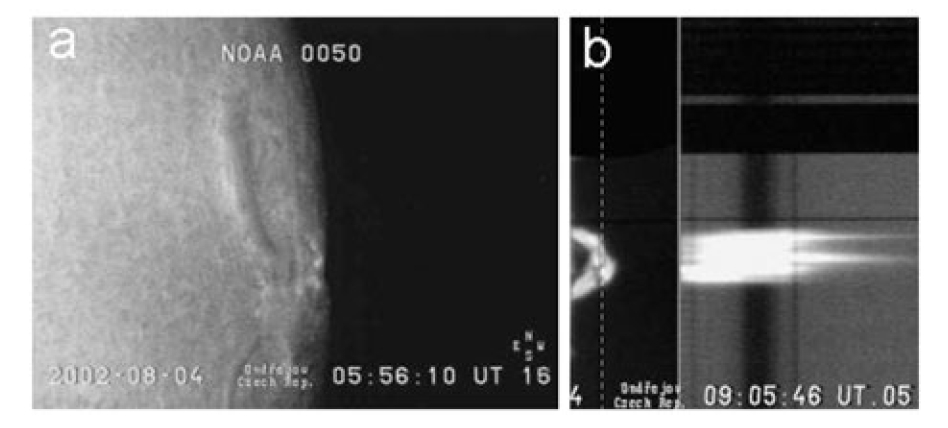
\includegraphics[width=0.9\textwidth]{img/td-setup/figure2fromHalpha.jpg}
	\caption{Observation of a limb event. $H\alpha$ slit-jaw is the middle (b) part, taken from \cite{miraClanek}.}
	\label{figure:observation}
	\end{center}
\end{figure}

For the modeling purposes, we are interested in the so-called $H\alpha$ slit-jaw which is the side-view of the magnetic flux tube during its evolution.
\paragraph{}
In order to model this phenomena physically, and geometrically, we utilize the magnetic field model by Titov and Demoulin (\cite{td}) which describes a twisted flux tube as part of a torus with minor radius $a$ (being the radius of the tube, not shown in \cref{figure:td}) and major radius $R$ submerged below the photosphere of the Sun by $d < R$, oriented as in \cref{figure:td} (taken from \cite{td}) with total current $I$.
\paragraph{}
The magnetic configuration is kept in a global equilibrium by the action of the Lorentz force due to the overlying magnetic field. The sources of this ambient field are modeled by a sub-photospheric line current $I_0$ and a pair of magnetic charges $+q, -q$ located at distance $L$ from the center of the torus, all located at the major axis of the torus.

\begin{figure}[H]
	\begin{center}
		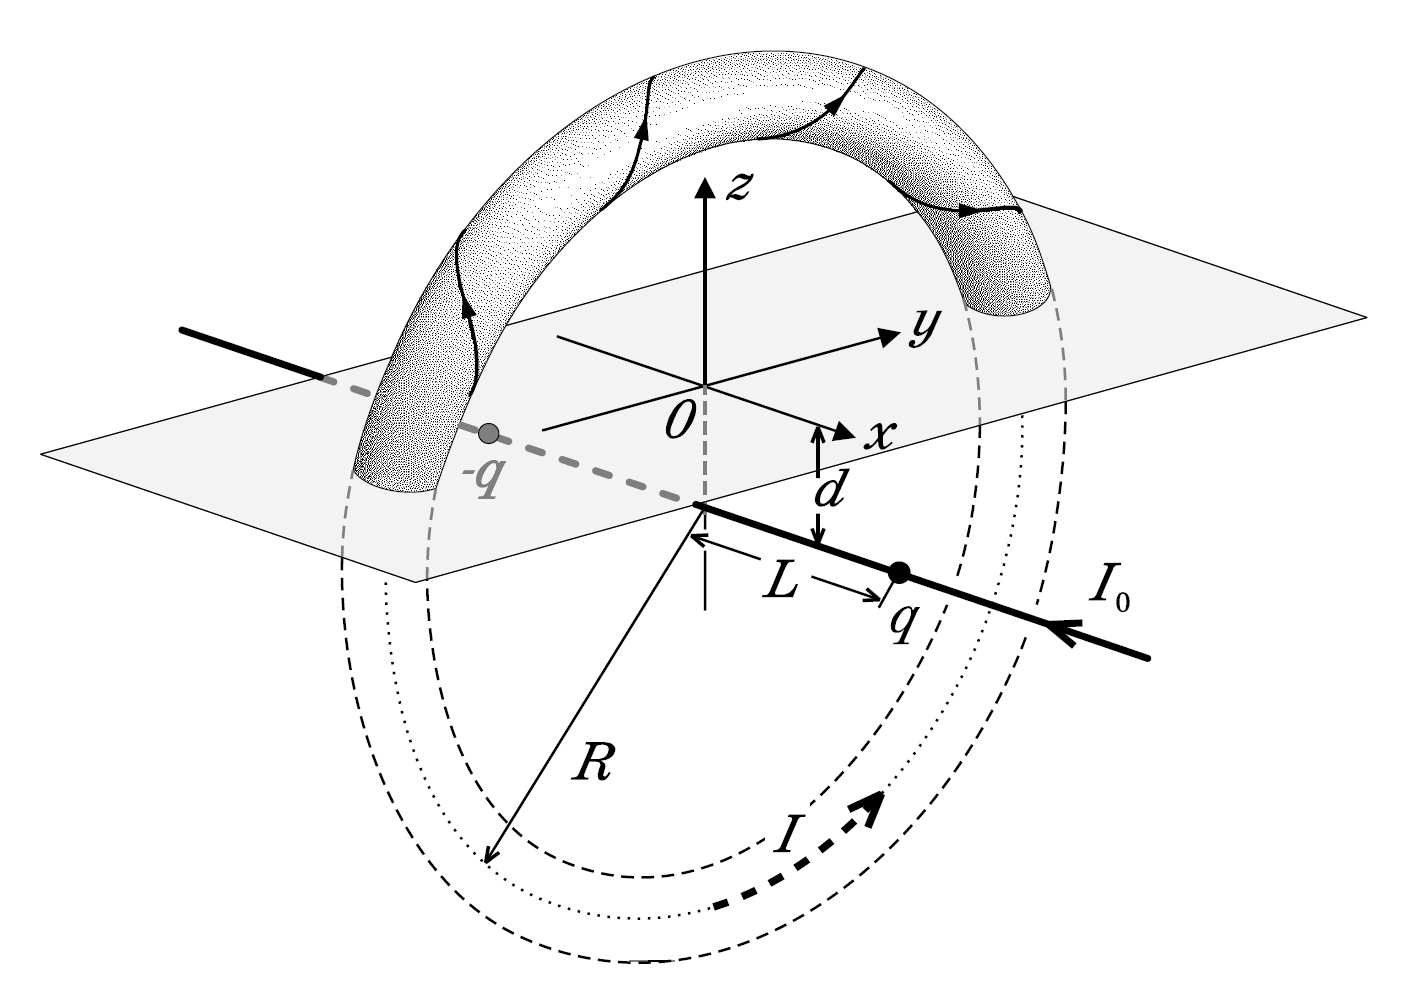
\includegraphics[width=0.9\textwidth]{img/td-setup/fromTD.jpg}
	\caption{The magnetic field under study, taken from \cite{td}.}
	\label{figure:td}
	\end{center}
\end{figure}

This geometrical/physical model needs to be properly modeled mathematically (including proper boundary conditions), then approached numerically, and finally computed using software that - in order to achieve reasonable accuracy of the solution - needs to be precisely implemented, must utilize approaches common in the high performance computing (HPC) field, and must be heavily optimized.
\paragraph{}
In the article \cite{miraClanek} which is a reference paper for this work, the model was set up according to observations, and numerical approach of Finite Difference Method (FDM) was used. The results obtained there are presented in \cref{figure:miraResult0,figure:miraResult14}, and in order to compare them with \cref{figure:observation}, also in the form in \cref{figure:miraResultToCompare} - where the colors are mapped to black and white to be comparable with the observation.

\begin{figure}[H]
	\begin{center}
		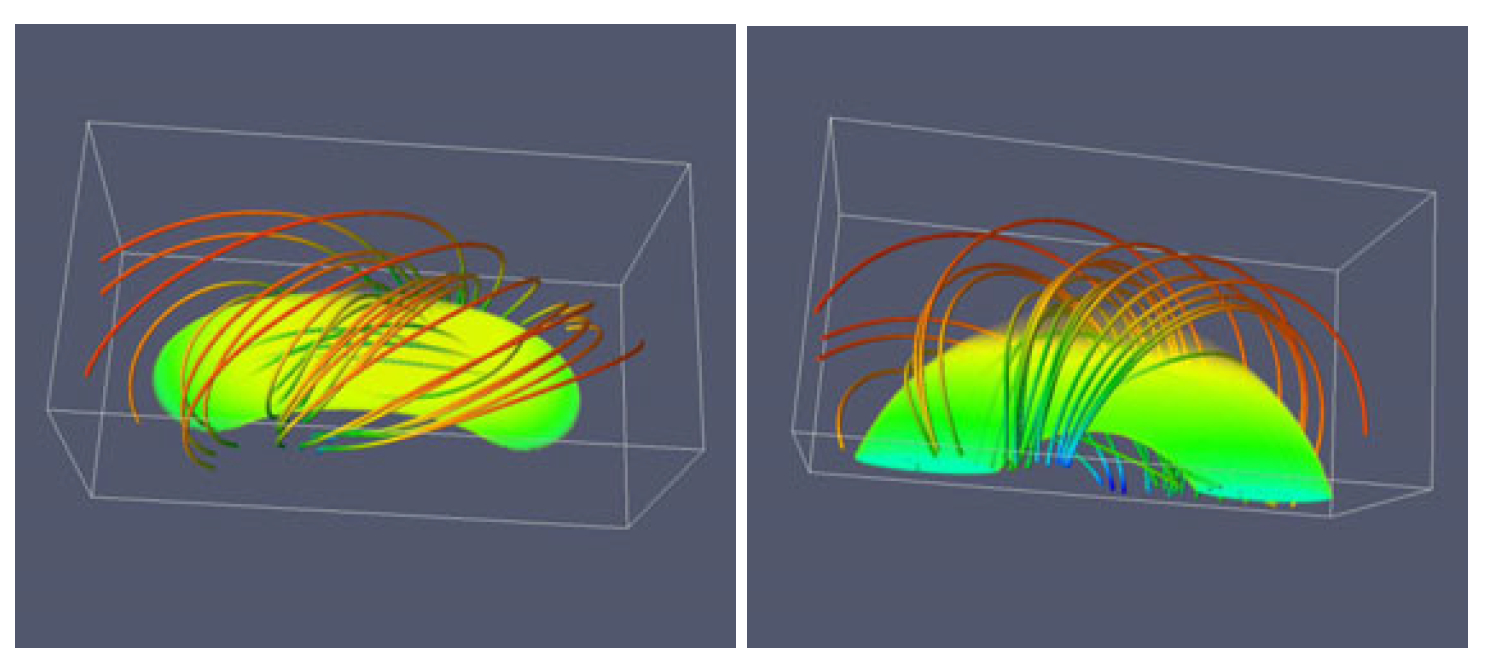
\includegraphics[width=0.9\textwidth]{img/td-setup/fromHalpha-initialFD.jpg}
	\caption{Results from \cite{miraClanek}, initial state, density volume and magnetic field isolines - top \& side view.}
	\label{figure:miraResult0}
	\end{center}
\end{figure}

\begin{figure}[H]
	\begin{center}
		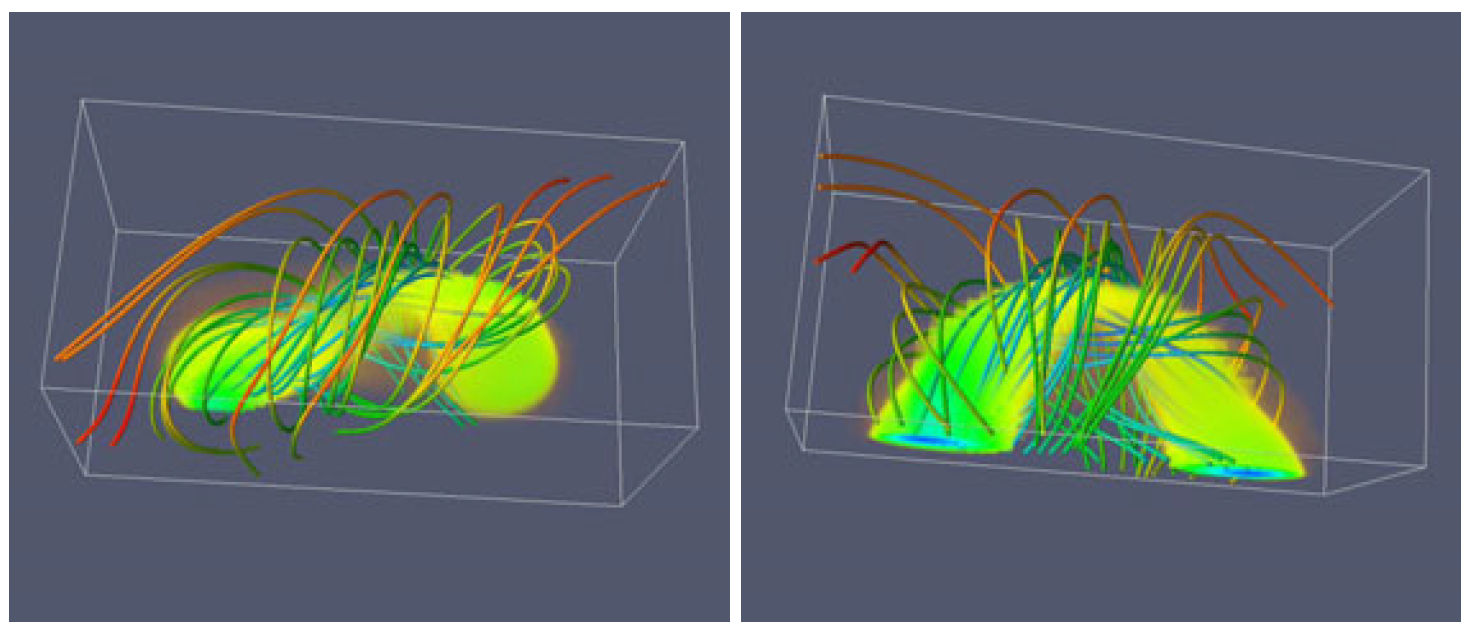
\includegraphics[width=0.9\textwidth]{img/td-setup/fromHalpha-14FD.jpg}
	\caption{Results from \cite{miraClanek}, state at $t = 14$, density volume and magnetic field isolines - top \& side view.}
	\label{figure:miraResult14}
	\end{center}
\end{figure}

\begin{figure}[H]
	\begin{center}
		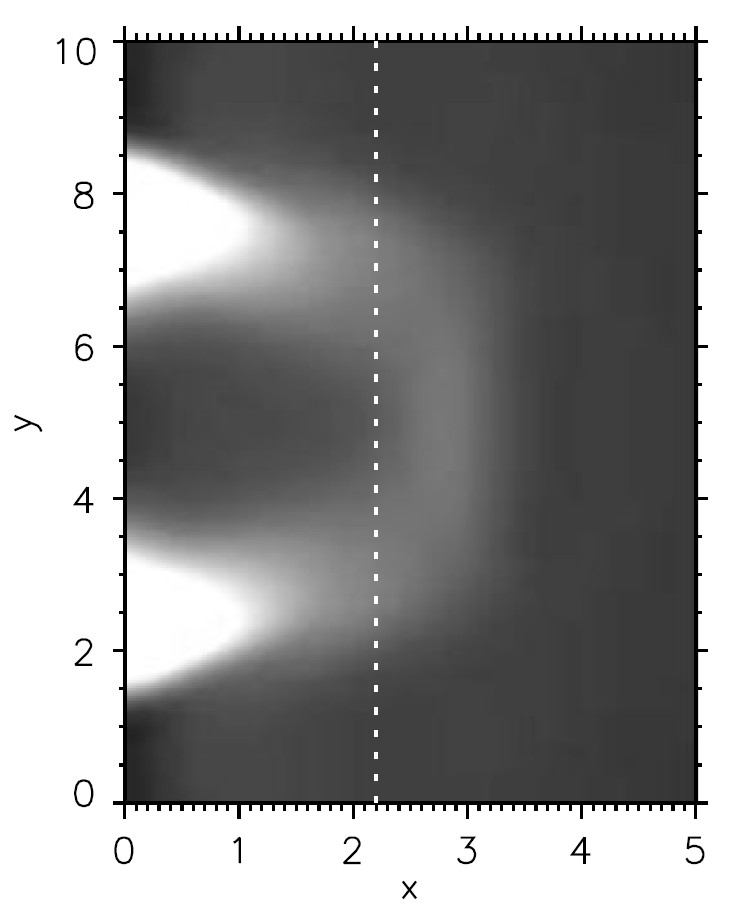
\includegraphics[width=0.5\textwidth]{img/td-setup/fromHalphaResult.jpg}
	\caption{Computed approximation of the observed event (\cref{figure:observation}), presented in \cite{miraClanek}.}
	\label{figure:miraResultToCompare}
	\end{center}
\end{figure}

The aim of this work is to be able to compute results of such problems with much higher resolution, and more importantly to implement a generic solver which can handle any similar problem with arbitrary geometric and physical parameters.

\subsection{Magnetic reconnection and other phenomena}
An additional topic, interesting from the astrophysical point of view and related to magnetohydrodynamics, is the magnetic reconnection.
\paragraph{}
Magnetic reconnection occurs within electrically charged gases called plasmas. These charged particles interact strongly with the magnetic field, but at the same time their motions modify the magnetic field. Under normal conditions, the magnetic field lines inside plasmas don't break or merge with other field lines. But sometimes, as field lines get close to each other, the entire pattern changes and everything realign into a new configuration. The amount of energy released can be formidable. Magnetic reconnection taps into the stored energy of the magnetic field, converting it into heat and kinetic energy that sends particles streaming out along the field lines. Solar flares, which are among the phenomena which are the most important to study, are driven by magnetic reconnection - and thus studying magnetic reconnection is of great importance.
\paragraph{}
From the numerical perspective, to investigate such phenomena is to bring the complexity of multiple scales present in the physical world - magnetic reconnection occurs at substantially different scales than e.g. the solar flares. To handle this numerically with adequate resolution, and reasonable computational costs, the implementation must be able to limit the number of degrees of freedom used for the discretization to such that yield the largest accuracy increase - namely, in this work, this is achieved via a state-of-the-art Adaptive Mesh Refinement approach.

\section{Aim of this work}
Main goal that was set for this work is implementation of a software package, capable of numerically solving the Magnetohydrodynamic equations with the following attributes:
\begin{itemize}
	\item The code must implement mathematically correct and clean methods, preferably with no parameter-dependent algorithms
	\item The code must allow for a broad spectrum of solution attributes occuring (shocks, oscillations, high energies, ...)
	\item The code must be able to capture very fine details of the solution through higher resolution, in reasonable computing time
	\item The code must be able to run a large-scale simulations, for which a single computer is not sufficient, and utilization of modern distributed computing approach is a must
	\item The code must be easy to use for the physicists, must be written using industry-standard modern object-oriented programming language
\end{itemize}
\paragraph{}
In order to achieve this, the work is divided into several logically successive steps. First, the mathematical model is clearly constructed, and its formulation translated into a form suitable for the chosen numerical method (the Discontinuous Galerkin method) of solving a system of PDEs - which was chosen in order to deliver the first and second of the above requirement (handling sharp fronts, discontinuities and the like with mathematical cleanliness) - is described afterwards.
\paragraph{}
The Discontinuous Galerkin method (DG) is then described in detail, in the entire process from the integral equations down to algorithms performing basic operations. Pitfalls of the numerical solution of the MHD equations (divergence constraint, slope limiting), and chosen way of solving them is given next, while still keeping the above requirements in mind.
\paragraph{}
Lastly, the biggest challenge is the satisfaction of the requirement of both the fine resolution of the solution, and the capability of running large-scale simulations on modern distributed computing architecture - while still providing all the other attributes of the implemented code. The approach to this, which involves mainly the Adaptive Mesh Refinement technique (AMR) together with Domain Decomposition technique, is presented after. And finally the verifications, and benchmarks and actual usage on an astrophysical problem are presented.


\section{State of the art}
Only recently, the scientific computation community, due to the advances in computer and supercomputer capabilities, has started with non-trivial numerical simulations of such complex physical phenomena that the MHD model describes. Since both for industrial applications, and obviously for astrophysical application of the MHD model, it is quite expensive (or downright impossible) to perform any experiments, the benefit of being able to simulate the phenomena on a computer is very large.\\
There exist several available numerical simulation codes, such as \citep{athena}, \citep{zeus}, \citep{ramses}, \citep{honzaFD}. These codes have been successfully applied to a range of problems in astrophysics.\\
There are many numerical methods implemented in these codes, such as the finite difference method (\citep{honzaFD}), finite volume method (\citep{ramses}), and the (continous) finite element method (\citep{honzaFem}).

There have been some attempts to employ also the discontinuous Galerkin method (\citep{mhdDg}, \citep{mhdDg2}), but so far no open-source generic software employing this method is available. Moreover, as the astrophysical interest lies in multi-scale problem, a software that can handle such problems would be much more beneficial. An approach that can achieve this capability of solving multi-scale problems is the Adaptive Mesh Refinement technique (AMR). What we understand under this term is not only a mesh refinement that is local (i.e. non-uniform), but a mesh refinement that does not originate in the problem description, and neither is invoked programatically with user input. The term 'adaptivity' means that through a predefined \textit{refinement indicator}, which is a function operating on the set of elements of the triangulation, elements to be refined are chosen automatically. This \textit{refinement indicator} is calculated from the solution, and in effect makes the triangulation 'adapt' to the solution - hence, AMR.

The reason for the development of a new code is two-fold. First, there is a unique collaboration between the Astronomical Institute of the Czech Academy of Sciences and the University of West Bohemia, where astrophysicists work together with electrical engineers (from theoretical and numerical modeling backgrounds), and the developed code will be usable for both simulating of astrophysical MHD phenomena, and industrial MHD applications.
\paragraph{}
Second, the newly developed code is based on locally-adaptive Discontinuous Galerkin method, which yields several advantages over the existing codes (which use e.g. finite difference, or finite volumes methods) developed at institutions of such high quality as \emph{Princeton} - \citep{athena}, \citep{zeus}. The advantages are especially of performance, and automation nature - method of higher order together with AMR yields results qualitatively and quantitatively comparable to low order uniform mesh methods, but with computational cost that can easily be an order of magnitude smaller. Automation is mentioned here related to the AMR, which, without user interaction, can optimize the computational triangulation for a particular time instance in the evolution of the modeled phenomena.
\paragraph{}
Another benefit (namely over \citep{zeus})of the newly created software are the use of modern object-oriented programming techniques and experience gained on creating finite element software (\citep{ja1}, \citep{ja2}, \citep{ja3}).
The implementation related to this work is written in the C++ language, with the use of existing software packages that are proven, and used by a wide community of researchers all over the world - deal.II (\citep{deal}), Trilinos, P4EST, Intel Parallel Studio, UMFPACK (\citep{umfpack}), Paraview(\url{http://www.paraview.org/}), and others.

\paragraph{}
The state of the art of numerical simulation of magnetohydrodynamics can be summarized as a state when the mathematical theory of the equations is quite solid, but the methods to solve the equations numerically in the most optimal and fast way are still being improved. The numerical solution is not merely about theoretical convergence rates and attributes of the particular method, but also the actual implementation plays an important role - i.e. programming, hardware, and software, and execution, both before, during, and very importantly after the actual method invocation (of the so-called \textit{postprocessing} of results). In all aspects of implementation, there is space for new approaches, new ideas, new milestones, that can expand the capabilities of today's numerical solution of magnetohydrodynamics phenomena.

\section{Notation}
Overview of notation used in the text is given in \Cref{table:notation}.
\begin{table}[H]
    \centering
    \begin{tabular}{ |c|l| } 
        \hline
        Symbol & Meaning \\ 
        \hline
        $a$ & a scalar quantity "a"\\
        $\bfa$ & a 3-element vector "a"\\
        $a_i$ & the i-th component of a vector $\bfa$ \\
        $\mrA$ & an 8-element vector "A" \\
        \hline
        $\rho$ & Density \\ 
        $\bfpi$ & Momentum \\ 
        $\mu$ & Permeability \\ 
        $\mu_0$ & Permeability of vacuum\\ 
        $t$ & Time variable\\ 
        $\bfx = \lo x, y, z\ro$ & Space variable \\ 
        $p$ & Pressure \\ 
        $\bfu$ & Velocity \\ 
        $u$ & Magnitude of velocity, i.e. $|\bfu|$ \\ 
        $\bfB$ & Magnetic flux density \\ 
        $\bfJ$ & Current density\\ 
        $B$ & Magnitude of magnetic flux density, i.e. $|\bfB|$ \\ 
        $\bfE$ & Electric field\\ 
        $e$ & Internal energy density \\ 
        $c$ & Speed of light\\ 
        $\bfg$ & Gravitational acceleration\\ 
        $\sigma$ & Conductivity, $\sigma = \frac{1}{\eta}$\\ 
        $\eta$ & Electrical restisistivity, $\eta = \frac{1}{\sigma}$\\
        $c_v$ & Specific heat at constant volume\\
        $c_p$ & Specific heat at constant pressure\\
        $\gamma$ & Poisson adiabatic constant\\
        $\theta$ & Absolute temperature\\
        $\bfq$ & Heat flux\\
        $q$ & Electric charge\\
        $\bff$ & Density of force acting on fluid\\
        $\bfF_L$ & Lorentz force, $\bfF_L = q\lo\bfE + \bfu\times\bfB\ro$\\
        $\bff_L$ & Lorentz force density, $\bff_L = \rho_q\bfE + \bfJ\times\bfB$\\
        $\varepsilon$ & Electrical permittivity\\
        $\varepsilon_0$ & Electrical permittivity of vacuum\\
        $\rho_q$ & Charge density\\
        $U_k$ & Kinetic energy\\ 
        $U_m$ & Magnetic energy\\ 
        $U$ & Total energy, $U = U_k + U_m + \rho e$ \\ 
        $\tilde{U}$ & Hydrodynamic energy, $\tilde{U} = U - U_m$ \\ 
        $\bfn$ & Unit outer normal\\
        \hline
    \end{tabular}
    \caption{Notation}
	\label{table:notation}
\end{table}
Here
\be
\label{magU}
U_m\lo\bfx, t\ro = \frac12 \sum_{i = 1}^{3}\bfB_i\lo\bfx, t\ro
\ee
is the magnetic energy,
\be
\label{kinU}
U_k\lo\bfx, t\ro = \frac12 \sum_{i = 1}^{3}\bfu_i\lo\bfx, t\ro
\ee
is the kinetic energy, and the relationship between the Total energy $U$ and pressure $p$ reads
\be
\label{presU}
U\lo\bfx, t\ro = \frac{p\lo\bfx, t\ro}{\gamma - 1} + U_m\lo\bfx, t\ro + U_k\lo\bfx, t\ro.
\ee
Note that in the text, indices $1, 2, 3$, and $x, y, z$ will be used interchangeably.


\chapter{Mathematical model}
In this chapter, the mathematical model will be derived from basic equations governing the studied physical phenomena, its weak formulation will be presented, and the complete mathematical problem which is solved will be described.
\section{Derivation of the mathematical model}
In order to derive the mathematical model, we first need to establish the basics - time-space frame (\Cref{subsec:init}), assumptions (\Cref{subsec:assump}), then we will start with the known Euler equations of compressible flow (\Cref{subsec:euler}, derivation of which is given e.g. in \cite{diplomka}), and by adding the Maxwell's equations (\Cref{subsec:maxwell}), we will derive the mathematical model for Magnetyhodrodynamics in the complexity needed  for handling problems presented in the introduction.
\subsection{Initial setup}
\label{subsec:init}

We consider a time interval $\left(0,T\right)$ and space domain $\Omega_{t}\subset \mathbb{R}^3$ occupied by a fluid at time $t$.
By $\mathcal{M}$ we denote the space-time domain in consideration: 
\begin{equation}\label{M}
\mathcal{M}=\left\{\left(\textbf{\textit{x}},t\right);\\\textbf{\textit{x}}\in\Omega_{t},t\in\left(0,T\right)\right \}.
\end{equation}
Moreover we assume that $\mathcal{M}$ is an open set.

\subsubsection{Assumptions}
\label{subsec:assump}
When dealing with MHD phenomena in plasma, the following rules apply
\begin{itemize}
    \item We assume that the fluid is inviscid.
    \item We assume that the fluid is compressible.
    \item We consider only the so-called \textit{perfect gas} or \textit{ideal gas} whose state variables satisfy the following \textit{equation of state}
    \begin{equation}\label{start_therm}
    p = R\theta\rho,
    \end{equation}
    where $\rho$ denotes density, $\theta$ denotes the absolute temperature, and $R$ is the \textit{gas constant}, which is defined as 
    \begin{equation}
    R = c_p - c_v.
    \end{equation}
    In the above, $c_p, c_v$ are specific heats at constant pressure, and at constant volume.
\end{itemize}

\subsection{Euler's equations of compressible flow}
\label{subsec:euler}
This system of equation reads

\begin{align}
\label{ContinuityEq} \pds{\rho}{t} + \nabla\cdot\left(\bfpi\right) & =  0\\
\label{NSEq} \pds{\bfpi}{t} + \nabla\cdot\left(\bfpi\otimes\bfu\right)& =  \rho\bff - \nabla\,p,\\
\label{EnergyEq} \pds{\tilde{U}}{t} + \nabla\cdot\lo{\tilde{U}}\bfu\ro & =  \rho\bff\cdot\bfu \,-\,\nabla\cdot\lo{p}\bfu\ro + \nabla\cdot\bfq,
\end{align}
where $\bfpi$ is momentum, $p$ pressure, $U$ total energy. Moreover, $\bfu$ denotes velocity, $\bff$ density of the force acting on the fluid, and $\bfq$ is the heat flux. By $\otimes$, we denote the \textit{tensor product}:
\begin{displaymath}
\bs{a}\otimes\bs{b} =
\left(
\begin{array}{ccc}
a_1b_1 & a_1b_2 & a_1b_3 \\
a_2b_1 & a_2b_2 & a_2b_3 \\
a_3b_1 & a_3b_2 & a_3b_3
\end{array}
\right).
\end{displaymath}

Moreover, the following relations hold:
\begin{align}
\tilde{U} & =  \rho e + U_k,\\
p & =  \lo{}\gamma-1\ro\lo{\tilde{U}}-U_k\ro, \label{therm_1}\\
\theta & =  \lo{\tilde{U}}/{\rho}-\left|\bfu\right|^2/2\ro/{c_v}.
\end{align}

This system is simply called the \textit{compressible Euler equations} for a heat-conductive perfect gas. The individual equations are called the \textit{continuity equation}(\Cref{ContinuityEq}), the \textit{Navier-Stokes equations} (\Cref{NSEq}), and the \textit{energy equation} (\Cref{EnergyEq}).

For the force density $f$ we assume that only the Lorentz force and gravity act upon the fluid:
$$
\label{ForceEq} \bff = \bff_L + \bfg.
$$


\subsection{Maxwell's equations of electromagnetism}
\label{subsec:maxwell}
In this work, we use Maxwell's equations with the assumption of constant electrical permittivity, and constant permeability. This system of equation reads
\begin{align}
\label{Ampere} \nabla \times \bfB & =  \mu_0 \lo \bfJ + \varepsilon_0 \pds{\bfE}{t}\ro\\\
\label{Faraday} \nabla \times \bfE & =  -\pds{\bfB}{t}\\
\label{Gauss} \nabla \cdot \bfE & =  \frac{\rho_q}{\varepsilon_0}\\
\label{GaussMag} \nabla \cdot \bfB & = 0,
\end{align}
where $\bfB$ denotes magnetic flux density, $\bfE$ denotes electric field, $\bfJ$ denotes current density, $\varepsilon_0$ is permittivity of vacuum, and $\rho_q$ is electric charge density.
The individual equations are known as Faraday's law(\Cref{Faraday}), Ampere's law(\Cref{Ampere}), and Gauss's laws(\Cref{Gauss}, \Cref{GaussMag}).


\subsection{Derived relations between electromagnetic quantities}
Further relations that are useful when deriving the MHD equations are:
\begin{align}
\label{U_mEq} \frac{\text{d}}{\text{d}t} U_m & =  \frac{1}{\mu_0}\nabla \cdot \lo \bfB\times\bfE\ro - \bfE\cdot\bfJ,\\
\label{Ohm} \bfE & =  -u \times \bfB + \frac{\eta}{\mu_0}\bfJ,\\
\label{InductionEq} \pds{\bfB}{t} + \nabla \times \lo \bfB \times \bfu \ro & =  -\frac{1}{\mu_0} \nabla \times \lo \eta \nabla \times \bfB \ro,
\end{align}
where $\mu_0$ denotes permeability of vacuum, $\eta$ is resistivity, and $U_m$ is magnetic energy.
The equation \Cref{Ohm} is the differential form of the \textit{Ohm's law}, the equation \Cref{InductionEq} is the \textit{induction equation}.

Applying now \Cref{ForceEq} to \Cref{NSEq}, \Cref{EnergyEq}, we obtain:
\begin{align}
\label{NSEq1} \pds{\bfpi}{t} + \nabla\cdot\left(\bfpi\otimes\bfu\right)& =  \rho_q\bfE + \bfJ\times\bfB + \rho\bfg - \nabla\,p,\\
\label{EnergyEq1} \pds{\tilde{U}}{t} + \nabla\cdot\lo{\tilde{U}}\bfu\ro & =  \rho_q\bfE\cdot\bfu + \bfJ\times\bfB\cdot\bfu + \rho\bfg\cdot\bfu \,-\,\nabla\cdot\lo{p}\bfu\ro + \nabla\cdot\bfq.
\end{align}
The adjusted energy equation \Cref{EnergyEq1} does not include the magnetic energy $U_m$, which we do want to include in the MHD equations. To achieve this, we employ \Cref{U_mEq} - \Cref{InductionEq} and rearrange. After rearranging we obtain
\be
\label{EnergyEqPrefinal} \pds{U}{t} = -\nabla\cdot\left[\bfpi\lo \frac{u^2}{2} + e\ro + p \bfu - \frac{1}{\mu_0}\bfB\times\bfE\right] + \rho \bfg \cdot \bfu + \nabla\cdot\bfq.
\ee

\subsection{Simplifying assumptions}
In what follows, we will make several simplifying assumptions, according to which we will get a system of equations that will adequately respect the physical model, yet will be easier to be solved.
\subsubsection{Negligible time derivative of electric field}
For the time increments that we are concerned with, the time derivative in \Cref{Ampere} (the so-called \textit{Maxwell's displacement current}) is
very small. To estimate the minimum time increment value $\tau$ which would allow us to neglect the derivative, take the ratio of the two terms on the right hand side of \Cref{Ampere}:
\begin{equation}
\varepsilon_0 \frac{\pds{\bfE}{t}}{\bfJ} \approx \frac{\frac{\varepsilon_0 \bfE}{\tau}}{\sigma\bfE} \approx \frac{\varepsilon_0}{\sigma \tau} \approx \frac{10^{-11}}{\tau}.
\end{equation}
This means for time scales much greater than $10^{-11}$ seconds, the time derivative of $\bfE$ can be neglected. As a consequence Equation \Cref{Ampere} can be written as:
\begin{equation}
\label{Assumption1} \nabla \times \bfB = \mu_0 \bfJ.
\end{equation}
Using \Cref{Assumption1}, we can write
\begin{equation}
\label{Asssumption11} \mu_0 \bfJ \times \bfB = \lo\bfB\cdot\nabla\ro\bfB - \nabla\frac{B^2}{2} = \nabla\cdot\lo\bfB\bfB\ro - \nabla\frac{B^2}{2},
\end{equation}
where the last equality comes from \Cref{GaussMag}. And using \Cref{Asssumption11} we can rewrite \Cref{NSEq1} as
\be
\label{NSEq2} \pds{\bfpi}{t} + \nabla\cdot\left(\bfpi\otimes\bfu\right) =  q\bfE + \nabla\cdot\lo\frac{1}{\mu_0}\bfB\bfB - \frac{B^2}{2}\mathrm{I}\ro + \rho\bfg - \nabla\,p
\ee

\subsubsection{Negligible electric field in the Navier-Stokes equations}
The magnitude of electric field is smaller than the magnetic field by the factor $\frac{u^2}{c^2}$, so we can neglect the term $\rho_q\bfE$ on the right-hand-side of \Cref{NSEq2}.

\subsubsection{Negligible heat fluxes}
Since the heat transfer accounts for a negligible contribution to the overall energy transfer, we neglect the heat flux terms, i.e. we set $\bfq = \mathbf{0}$ in the energy equation \Cref{EnergyEqPrefinal}.

\subsection{Adding the induction equation}
The induction equation \Cref{InductionEq} can be rearranged in the following way:
\begin{align}
\pds{\bfB}{t} + \nabla \times \lo \bfB \times \bfu \ro & =  -\frac{1}{\mu_0} \nabla \times \lo \eta \nabla \times \bfB \ro\\
\label{InductionPreFinal} \pds{\bfB}{t} & =  - \nabla \times \lo \bfu \otimes \bfB - \bfB \otimes \bfu \ro + \frac{1}{\mu_{0}\sigma} \lo \nabla^2 \bfB \ro.
\end{align}
Now we can form the system of MHD equations:
\begin{align}
\label{ContinuityEqFinal} \pds{\rho}{t} & =  - \nabla\cdot\left(\bfpi\right),\\
\label{NSEqFinal} \pds{\bfpi}{t} & =  - \nabla\cdot\left(\bfpi\otimes\bfu\right) + \nabla\cdot\lo\frac{1}{\mu_0}\bfB\bfB - \frac{B^2}{2}\mathrm{I}\ro + \rho\bfg - \nabla\,p,\\
\label{EnergyEqFinal} \pds{U}{t} & =  -\nabla\cdot\left[\bfpi\lo \frac{u^2}{2} + e\ro + p \bfu - \frac{1}{\mu_0}\bfB\times\bfE\right] + \rho \bfg \cdot \bfu\\
\label{InductionFinal} \pds{\bfB}{t} & =  - \nabla \times \lo \bfu \otimes \bfB - \bfB \otimes \bfu \ro + \frac{1}{\mu_{0}\sigma} \lo \nabla^2 \bfB \ro.
\end{align}
This form suggests that rewriting these equations into a more suitable (for numerical calculations) conservative form shall be possible.
\subsection{Conservative form of the MHD equations}
A conservative form of a system of equations takes the form of
\be
\label{conservativeGeneric} \pds{\mrPsi}{t} + \nabla \cdot \mrF\lo\mrPsi\ro = \mrS,
\ee
where $\mrPsi$ is the so-called \textit{state vector}, $\mrF_i,\ i = 1, 2, 3$ are the so-called \textit{fluxes}, and $\mrS$ is the so-called \textit{source term}.
\paragraph{}
Rewriting the system of equations \Cref{ContinuityEqFinal} - \Cref{InductionFinal} to the form \Cref{conservativeGeneric} is fairly straightforward.
We obtain the following:
\begin{align}
\mrPsi & =  \lo\begin{array}{c}\rho \\ \pi_1 \\ \pi_2 \\ \pi_3 \\ U \\ B_1 \\ B_2 \\ B_3 \\ \end{array}\ro,\\\mrF_i & =  \lo\begin{array}{c} \pi_i \\ \frac{\pi_1 \pi_i}{\rho} - B_1 B_i + \frac12 \delta_{1i} \lo p + U_m\ro \\ \frac{\pi_2 \pi_i}{\rho} - B_1 B_i + \frac12 \delta_{2i} \lo p + U_m\ro \\ \frac{\pi_3 \pi_i}{\rho} - B_1 B_i + \frac12 \delta_{3i} \lo p + U_m\ro \\ \frac{\pi_i}{\rho} \lo \frac{\gamma}{\gamma - 1} p + U_k\ro + 2\eta\varepsilon_{ijk} J_j B_k + \frac{2}{\rho} \varepsilon_{ijk} \lo \pi_k B_i - \pi_i B_k\ro B_j  \\ \frac{\pi_i B_1 - \pi_1 B_i}{\rho} + \eta \varepsilon_{1ij} J_j \\ \frac{\pi_i B_2 - \pi_2 B_i}{\rho} + \eta \varepsilon_{2ij} J_j \\ \frac{\pi_i B_3 - \pi_3 B_i}{\rho} + \eta \varepsilon_{3ij} J_j \\ \end{array}\ro,\\
\mrS & =  \lo\begin{array}{c}0 \\ \rho g_1 \\ \rho g_2 \\ \rho g_3 \\ \bfpi \cdot \bfg \\ 0 \\ 0 \\ 0 \\ \end{array}\ro,
\end{align}
where $J_j = \lo\nabla\times\bfB\ro_j$, $\varepsilon_{ijk}$ is the Levi-Civita symbol, and $\delta_{ij}$ the Kronecker delta.
\subsection{Solution considerations}
For mathematical clarity, we should state, that the solution to the equations \Cref{conservativeGeneric} is such a function
\be
\label{HardSln} \mrPsi\in C^1\lo\lo0, T\ro, \left[C^1\lo\Omega_{t}\ro\right]^8\ro;\ \mrPsii\in C^1\lo\lo0, T\ro, C^2\lo\Omega_{t}\ro\ro,\,i = 6, 7, 8,
\ee
for which \Cref{conservativeGeneric} holds for all $\bfx\in\Omega_t,\ t\in\lo 0, T\ro$. The kind of spaces we used in the definition is called the Bochner spaces.
\paragraph{}
Because such a requirement on the solution $\mrPsi$ is rather strong, we shall instead look for a so-called \textit{weak solution}, which is specified in the coming sections.

\section{Weak formulation of the problem}
The DG method is defined by first considering the weak formulation of the equations \ref{conservativeGeneric} obtained by multiplying the equations at every time instance $t$ by a (vector-valued) test function $\mrv\in W_t$, where $W_t$ is a suitable space of (vector-valued) functions $W_t = \lo W_1, ..., W_8\ro$, integrating over the space domain $\Omega_{t}$, and performing integration by parts.
We start with multiplying \ref{conservativeGeneric} by a test function:
\be
\pds{\mrPsi}{t} \mrv + \lo\nabla \cdot \mrF\lo\mrPsi\ro\ro \mrv = \mrS \mrv,
\ee
then we integrate over $\Omega_{t}$:
\be
\int_{\Omega_{t}} \pds{\mrPsi}{t} \mrv + \int_{\Omega_{t}} \lo\nabla \cdot \mrF\lo\mrPsi\ro\ro \mrv = \int_{\Omega_{t}} \mrS \mrv,
\ee
and finally we integrate by parts:
\be
\label{WeakFinal} \int_{\Omega_{t}} \pds{\mrPsi}{t} \mrv - \int_{\Omega_{t}}\mrF\lo\mrPsi\ro \lo\nabla \cdot \mrv\ro + \int_{\partial\Omega_{t}} \lo\mrF\lo\mrPsi\ro \cdot \bfn \ro\mrv = \int_{\Omega_{t}} \mrS \mrv,
\ee
where the terms $\mrF\lo\mrPsi\ro \lo\nabla \cdot \mrv\ro; \lo\mrF\lo\mrPsi\ro \cdot \bfn \ro\mrv$ are meant as a component-wise multiplication.
\paragraph{}
Now without going into detail, we can conclude, that a suitable space $W$ would be
\be
\label{Sobolev} W_t = \left[H^{1}\lo\Omega_t\ro\right]^8,
\ee
and we shall look for a solution to the \ref{WeakFinal} in the same space $W_t$ at every time instance $t$. We shall not relax the requirement for continuity of time-derivatives we imposed for the \textit{hard solution} \ref{HardSln} for reasons discussed later, and we arrive at the following Bochner space in which we are looking for a weak solution of \ref{conservativeGeneric}:
\be
\label{Bochner} W = C^{1}\lo\lo0, T\ro, W_t\ro.
\ee

To sum up we can define the \textit{weak solution $\mrPsi = \mrPsi\lo(t, \bfx\ro)$} of MHD equations \ref{conservativeGeneric} as
\begin{enumerate}
    \label{weakSlnDef}
    \item $\mrPsi\lo(t, \bfx\ro) \in W$ defined in \ref{Bochner}
    \item \ref{WeakFinal} holds for all $t\in\lo0, T\ro$, and all $\mrv\in W_t$.
    \item $\mrPsi\lo0, \bfx\ro = \Pi \mrPsi^0\lo\bfx\ro$,
\end{enumerate}
where $\Pi$ is a projection of the initial condition $\mrPsi^0$ onto $W_0$.

\section{Boundary conditions}
\label{section:bcs}
For the problem of finding the solution as described in \cref{weakSlnDef} to be complete, we need to specify the proper boundary conditions.
\subsection{Essential (inflow) boundary conditions}

Since the solution as described in \cref{weakSlnDef} of the problem specified in \cref{WeakFinal} is not influenced by its values on the boundary $\Omega_t$, we are not able to employ standard essential boundary conditions of the form $\bfu\left(x, y, z\right) = \bfu_D\left(x, y, z\right)$ with a known $\bfu_D$.
If such a condition is required from the physical nature of the described phenomenon (as often is the case), it is only implied by a correct definition of fluxes at the boundary - as one can see in the last integrand $\lo\mrF\lo\mrPsi\ro \cdot \bfn \ro\mrv$ in \cref{WeakFinal}. We shall see how that is numerically handled in later chapters.


\subsection{Outflow (do-nothing) boundary conditions}
If a particular boundary is only present in the numerical model (representing e.g. an "outer" boundary that is there to limit the size of the computation to the area of interest), that is, a free boundary, that is not in any way present as an actual physical boundary or interface, this is achieved by specifying that values of $\mrPsi$ do not change through the boundary in \cref{WeakFinal}:
\be
\label{bcoutdef}
\frac{\partial\mrPsi}{\partial\bfn} = 0.
\ee

\subsection{Periodic boundary conditions}
Periodic boundary condition is always specified on two parts $\Gamma_1, \Gamma_2$ of the domain boundary that share the bijection mapping between points:
\be
\label{periodicMapping}
\left[x_1, y_1, z_1\right] \leftrightarrow \left[x_2, y_2, z_2\right] \forall \left[x_1, y_1, z_1\right] \in \Gamma_1,\ \forall \left[x_2, y_2, z_2\right] \in \Gamma_2,
\ee
so that for each pair of related points $\left[x_1, y_1, z_1\right] \leftrightarrow \left[x_2, y_2, z_2\right]$, the values must be the same:
\be
\label{periodicBCs}
u\left(\left[x_1, y_1, z_1\right]\right) = u\left(\left[x_2, y_2, z_2\right]\right) \forall \left[x_1, y_1, z_1\right] \in \Gamma_1,\ \forall \left[x_2, y_2, z_2\right] \in \Gamma_2:\, \left[x_1, y_1, z_1\right] \leftrightarrow \left[x_2, y_2, z_2\right].
\ee


\chapter{Numerical approach}
The weak formulation of the problem we obtained in \ref{weakSlnDef} still posses a problematic attribute - the space defined in \ref{Bochner} is of infinite dimension, and therefore we would need to employ analytical methods to find the solution \ref{weakSlnDef} in such a space. The equation \ref{WeakFinal} is however rather impossible to be solved analytically, and we have to utilize some sort of numerical simulation - which in turn needs to operate on finite-dimensional spaces. But we need to make sure that the simplifying (reducing) assumptions we make on the way to the numerical model are acceptable so that the numerical solution we obtain converges (as we reduce the discretization size) to the solution defined in \ref{weakSlnDef}.

\paragraph{}
In this chapter we shall consider that $\Omega_t = \Omega\, \forall t \in \lo 0, T\ro $, i.e. the computational domain does not change with respect to time. There are approaches to numerical simulation of MHD phenomena without this condition in place, which utilize the exact same general approach described in this work plus they add additional steps in the algorithm. These are outside of the scope of this work. Also, we always take $\Omega \subset \mathbb{R}^3$.

\section{Triangulation}
\label{section:triangulation}
We start with leaving the time-derivative untouched, and focus on the discretization in space for now - we are performing a \textit{space semidiscretization}.
\paragraph{}
First step in the process of the discretization is to divide the computational domain $\overline{\Omega}$ into a finite number of subsets with properties described below. These subsets form the set, further denoted by $ T_h$, called the \textit{triangulation or mesh of the domain $\Omega$}. Please note that the terms \textit{triangulation} and \textit{mesh} shall be used in the text interchangeably. The parameter $h>0$ of the triangulation usually represents maximum of diameters of all elements $K\in T_h$. The elements $K\in T_h$ are in the context of the finite volume method called $finite\ volumes$.
\\\ \\Properties of $T_h$:
\begin{enumerate}
    \item Each $K\in T_h$ is closed and connected with its interior $K^{\circ}\neq\emptyset$.
    \item Each $K\in T_h$ has a Lipschitz boundary.
    \item$\cup_{K\in T_h}K\,=\,\overline{\Omega}$
    \item If $K_1,K_2\in T_h$, $K_1\neq{K_2}$, then $K_1^{\circ}\cap{T}_2^{\circ} = \emptyset$.
\end{enumerate}
\paragraph{}
In our case of the three-dimensional problem, we assume that the domain $\Omega$ is obtained as an approximation of the original computational domain (also denoted by $\Omega$), and the triangulation is chosen accordingly to the following attributes:
\renewcommand{\labelenumi}{\Alph{enumi})}
\begin{enumerate}
    \item Each $K\in T_h$ is a closed rectangular hexahedron, possibly with curved faces.
    \item For $K_1,K_2\in T_h,\,K_1\neq{K}_2$ we have either $K_1\cap{K}_2 = \emptyset$ or $K_1,K_2$ share one face (if the shared face is a whole common face, we call the triangulation \emph{regular}), or $K_1,K_2$ share one vertex, or $K_1,K_2$ share one face.
    \item$\cup_{K\in T_h}K\,=\,\overline{\Omega}.$
\end{enumerate}
Furthermore
\be
\label{Idef}  T_h = \left\{K^i, i\in I\right\},
\ee
where $I\subset Z^+ = \left\{0, 1, 2, ...\right\}$ is a suitable index set.\\
By $\Gamma_{ij}$ we denote a common face between two
neighboring elements $K^i$ and $K^j$. We set 
$$s
\lo i\ro = \left\{j\in I; K^j \text{ is adjacent to } K^i\right\}.
$$
The boundary $\partial\Omega$ is formed by a finite number of faces of elements $K^i$ adjecent to
$\partial\Omega$. We denote all these boundary faces by $S_j$, where $j\in I_b\subset Z^{-} = \left\{-1, -2, ...\right\}$.
Now we set 
$$
\gamma\lo i \ro = \left\{j\in I_b; S_j \text{ is a face of } K^i\in T_h\right\}
$$ 
and 
$$
\Gamma_{ij} = S_j\text{ for } K^i\in  T_h\text{ such that }S_j\subset\partial K^i, j\in I_b.
$$
For $K^i$ not containing any boundary face $S_j$ we set $\gamma\lo i \ro = \emptyset$.\\
Obviously, $s\lo i \ro \cap\gamma\lo i\ro = \emptyset$ for all $i\in I$. If we write $S\lo i \ro = s \lo i\ro \cup \gamma\lo i \ro$, we have
$$
\partial K^i = \cup_{j\in S\lo i \ro}\Gamma_{ij},\ \ \ \partial K^i\cap\partial{\Omega} = \cup_{j\in\gamma\lo i \ro}\Gamma_{ij}.
$$
Furthermore we define the set of internal (i.e. not lying on the boundary $\partial\Omega$) faces as
\be
\label{InternalEdges} \Gamma_I = \cup_{i\in I} \cup_{j \notin \gamma\lo i \ro} \Gamma_{ij},
\ee
and the set of boundary (i.e. lying on the boundary $\partial\Omega$) faces as
\be
\label{BndEdges} \Gamma_B = \cup_{i\in I} \cup_{j \in \gamma\lo i \ro} \Gamma_{ij}.
\ee
\paragraph{Note}
If we were to use not $\Omega\subset\mathbb{R}^3$, but rather $\Omega\subset\mathbb{R}^4$, we may just employ the following machinery also to the time-derivative - this is not an uncommon approach. Why the approach described in this work is favored by the author is twofold:
\begin{itemize}
    \item Data (in a general sense - e.g. algebraic systems, function bases, etc.) are smaller when using a separate handling for time-derivative
    \item The dependency on time and space may (and usually does) vary a lot for physical phenomena - to have a separate approach is therefore beneficial
\end{itemize}
\subsection{Distributed triangulation}
\label{section:ditributedTria}
The standard approach to handle large problems that are impossible to be calculated on a single processor in mesh-based numerical simulations (such as Discontinuous Galerkin method) is to employ a \textit{domain decomposition} method, where each of the processors on which the simulation runs holds data about a subset of elements of the mesh $T$.
Consequently, also the matrix and vector assembly (described in ~\Cref{algorithm:singleTimeStep}), the linear problem solution, slope limiting, and AMR procedures are performed by all processors using data they have available. The aim here is not to go into deep technical details of distributing data, etc.
\paragraph{}
In \Crefrange{figure:domainDecomposition}{figure:domainDecomposition2}, domain $\Omega = \left[0, 1\right] \times \left[0, 1\right] \times \left[0, 1\right]$ was used, it was triangulated by $10 \times 10 \times 10$ mesh elements and the domain was distributed among 5 processors labelled $0..4$.

\begin{figure}[H]
		\begin{center}
			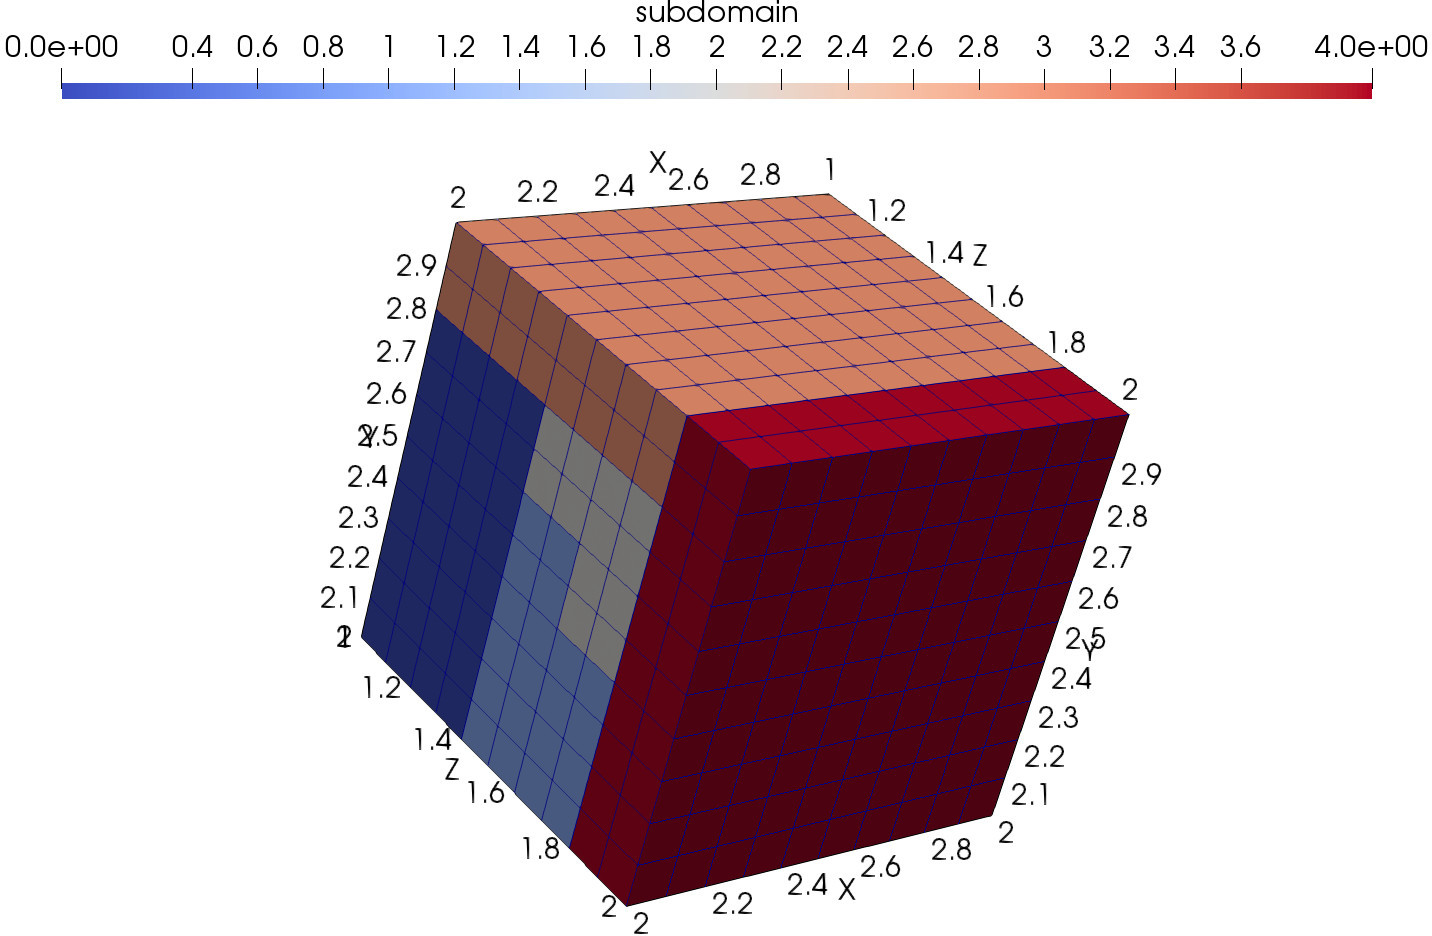
\includegraphics[width=0.78\textwidth]{img/mesh/cube.jpg}
			\vspace{-2mm}
		\caption{Cubical domain $\Omega$ with color-coded processor-owned elements.}
		\label{figure:domainDecomposition}
		\end{center}
	\end{figure}\vspace{-5mm}
	
\begin{figure}[H]
		\begin{center}
			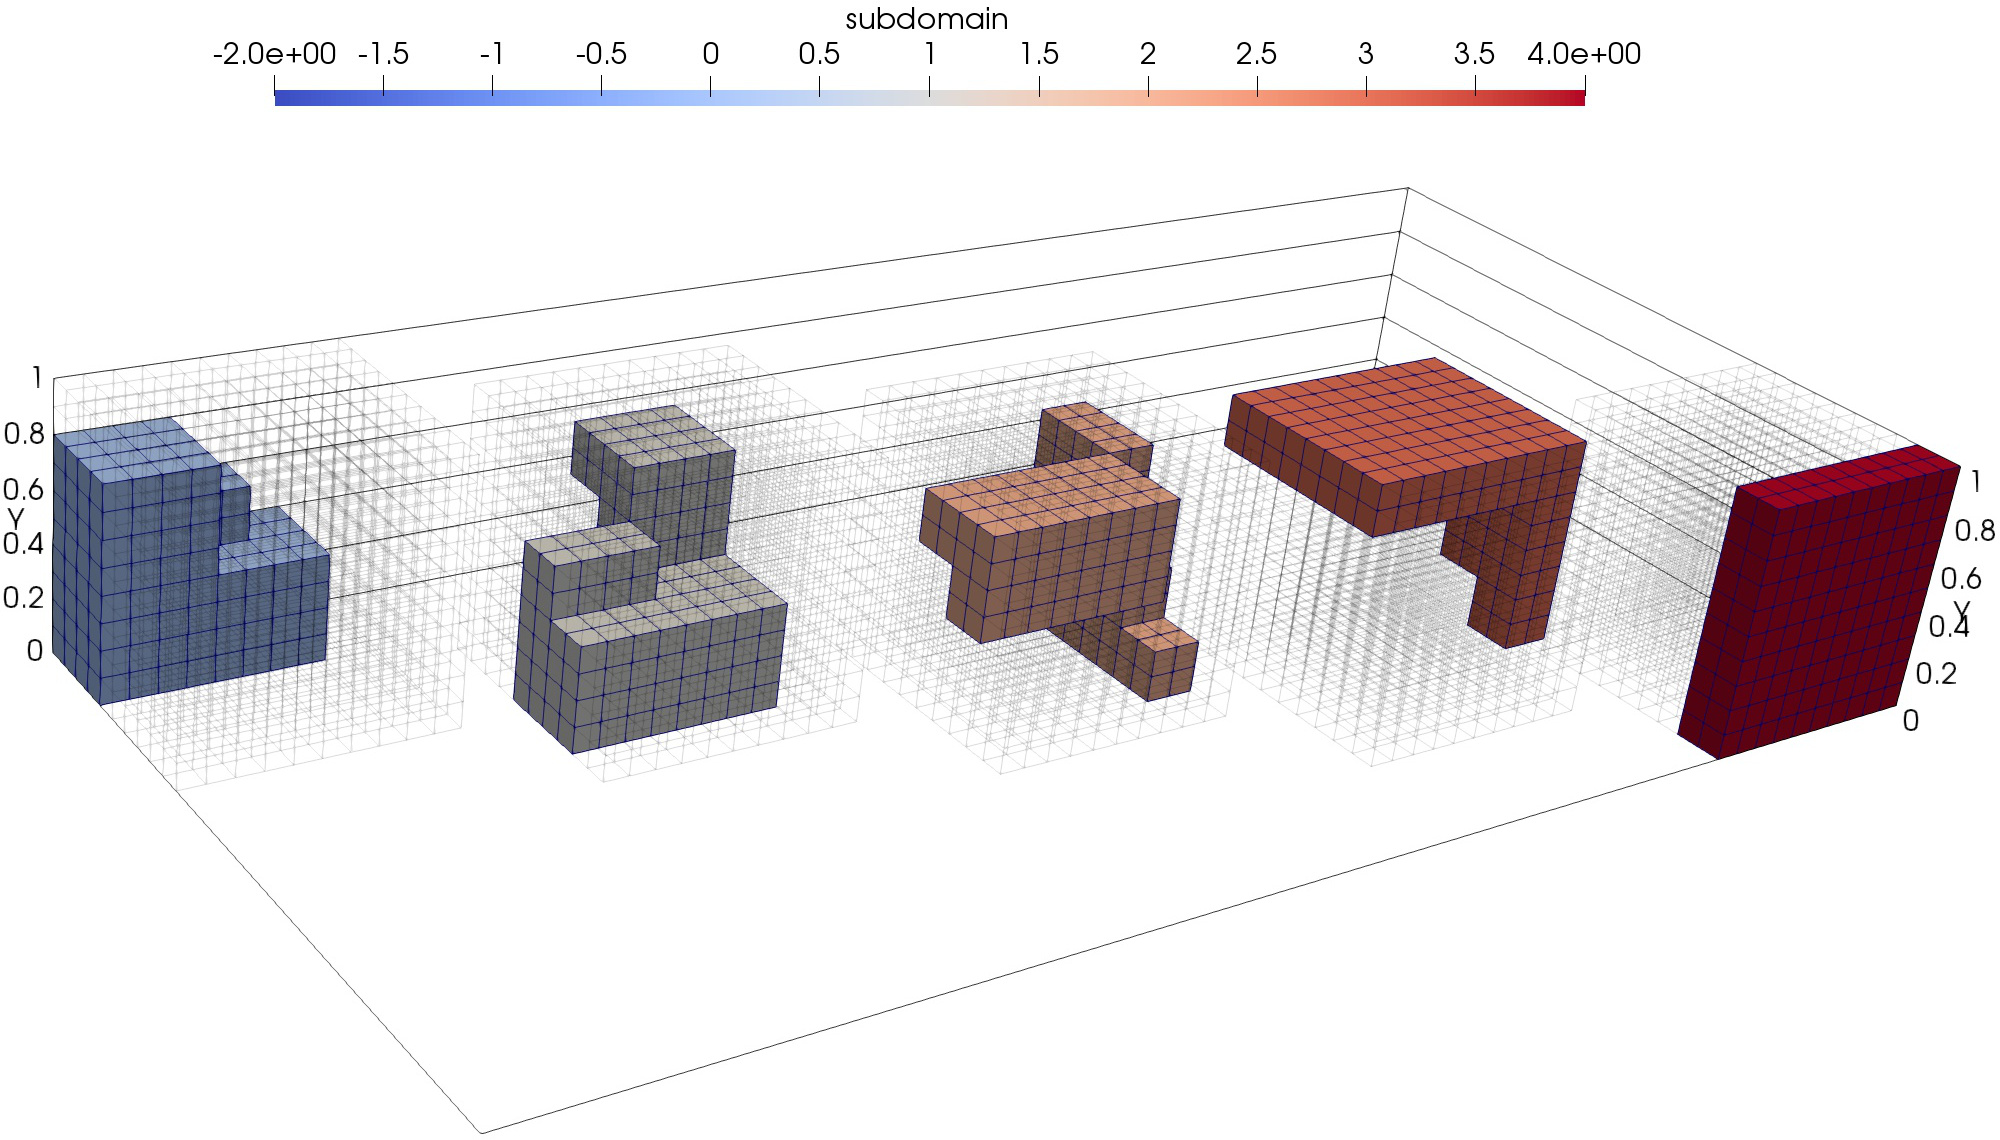
\includegraphics[width=0.78\textwidth]{img/mesh/cubeSub.jpg}
			\vspace{-2mm}
		\caption{The same domain as in \Cref{figure:domainDecomposition}, with clearer indication of elements that belong to individual processors (0..4 left to right).}
		\label{figure:domainDecomposition2}
		\end{center}
	\end{figure}\vspace{-5mm}
	

\section{Discontinuous Galerkin method}

For complex problems of compressible flow, and of course for even more complex problems of compressible MHD, there has been a number of attempts to use standard and well known Finite Element Methods that replace the spaces defined in \ref{Bochner} with finite-dimension spaces with bases formed by continuous piecewise polynomial functions. These attempts struggled with a common problem of spurious oscillations appearing in the solution - the origin of which is the lack of "stabilization", provided by the second-order terms in elliptic equations. Solution to these problems is the application of stabilization techniques, that usually introduce some sort of artificial diffusion (the second-order term), all of which are non-physical, and generally involve "magical" numbers - constants that are of pure computational nature (not a part of the physical description) or even worse are problem-specific.

\subsection{Overview of the DG method}
Due to this reason, there  was an effort to develop methods which would not need such stabilization techniques, and would still offer reasonable resolution of shockwaves, boundary and interior layers, and steep gradients without exhibiting spurious oscillations in the approximate solutions. The approach taken here is based on the idea to combine finite volume and Finite element methods leading to the so-called \emph{discontinuous Galerkin finite element method (DGFEM, DG)}. Here we shall derive and analyze DG for our equations. Let $T_h$ be a triangulation of $\Omega$. For each $K\in T_h$ we introduce the notation
\begin{eqnarray}
\partial K^- & = & \left\{x\in\partial K;\beta\lo\bs{x}\ro\cdot\bfn\lo\bs{x}\ro <0\right\},\\
\partial K^+ & = & \left\{x\in\partial K;\beta\lo\bs{x}\ro\cdot\bfn\lo\bs{x}\ro \geq 0\right\}.
\end{eqnarray}
By $H^1\lo\Omega, T_h\ro$ we denote the so-called \textit{broken Sobolev space}:
\be
\label{BrokenSobolev} H^1\lo\Omega,T_h\ro = \left\{v\in L^2\lo\Omega\ro;\ v|_K\in H^1\lo K\ro \forall K\in T_h\right\}.
\ee
This space is an approximation of the space defined in \ref{Sobolev}, but it contains functions that are discontinuous on element interfaces $\Gamma_ij$.
\paragraph{}
For $u\in H^1\lo\Omega,T_h\ro$ we set
\be
\label{PlusDef} u_K^+ = \text{trace of } u|_K \text{ on }\partial K
\ee
(i.e. the interior trace of $u$ on $\partial K$). For each face $E\subset\partial K\backslash\Gamma$ of $K$, there exists $K'\neq K,\ K'\in T_h$, adjacent to $E$ from the opposite side than $K$. Then we put
\be
\label{MinusDef} u_K^- = \text{trace of } u|_{K'} \text{ on } E.
\ee
In this way we obtain the exterior trace $u_K^-$ of $u$ on $\partial K\backslash\Gamma$ and define the jump of $u$ on $\partial K\backslash\Gamma$:
\be
[u]_K = u_K^+ - u_K^-.
\ee
\subsubsection{Approximation of the broken Sobolev space}
\label{section:Vh}
Let the domain $\Omega$ be covered with a mesh $T_h = 
\{ K_1,$ $K_2, \dots, K_M \}$ where each element $K_m$ carries an arbitrary
polynomial degree $1 \leq p_m$, $\forall m = 1, 2, \dots, M$. The broken Sobolev space 
$H^1\lo\Omega,T_h\ro$ will be approximated by a finite-dimensional space of picewise-polynomial functions
\be
\label{VH} V_{h} = \{ v \in L^2(\Omega); \ v|_{K_m} \in P^{p_m}(K_m)\ \mbox{for all}\ 1 \leq m \leq M \}
\ee
where $P^{p}$ is defined as
\bd
P^{p} = \mbox{span}\{\sum_{\substack{0\leq i, j, k \leq p \\i+j+k\leq p}}\alpha_i\ x_1^i\ x_2^j\ x_3^k,\ \ \alpha_i\in\mathbb{R} \}.
\ed

\subsection{DG formulation of MHD equations}
Although the resulting system will look very similar to the weak formulation \ref{WeakFinal}, the derivation makes more sense to be done starting with the \ref{conservativeGeneric}.
\paragraph{}
As stated in \ref{section:triangulation}, at this point we will discretize the problem in space, and leave the time-derivative untouched.
The approximate solution will be sought at each time instant $t$ as an element of the finite-dimensional space
$$
\left[V_h\right]^8,
$$
where $V_h$ is defined in \ref{VH}. Functions
$$
\mrvh \in \left[V_h\right]^8\approx \left[H^1\lo\Omega,T_h\ro\right]^8,
$$
where $H^1\lo\Omega,T_h\ro$ is defined in \ref{BrokenSobolev}, are in general discontinuous on interfaces $\Gamma_{ij}$.
By $\mrvh|_{ij}$ and $\mrvh|_{ji}$ we denote the values of $\mrvh$ on $\Gamma_{ij}$ considered from the
interior and the exterior of $K_i$, respectively. The symbols
$$
\left<\mrvh\right>_{ij} = \frac12 \lo \mrvh |_{ij} + \mrvh |_{ji}\ro,\ \left[\mrvh\right]_{ij} = \mrvh |_{ij} - \mrvh |_{ji}
$$
denote the average and jump of a function $\mrvh$ on $\Gamma_{ij}$.
In order to derive the discrete problem, we multiply \ref{conservativeGeneric} by a test function $\mrvh \in \left[V_h\right]^8$ in a component-wise fashion, integrate over any element $K_i \in T_h$, apply Green's theorem and sum over all $i \in I$, where $I$ is defined in \ref{Idef}:
\be
\label{DG1} \int_{\Omega_{t}} \pds{{\mrPsi_h}}{t} \mrvh - \sum_{K_i \in T_h}\int_{K_i}\mrF\lo{\mrPsi_h}\ro \lo\nabla \cdot \mrvh\ro + \sum_{K_i\in T_h} \sum_{j\in s_i} \int_{\Gamma_{ij}} \lo \mrF\lo{\mrPsi_h}\ro \cdot \bfn_{ij} \ro \mrvh = \int_{\Omega_{t}} \mrS \mrvh,
\ee
where $\bfn_{ij}$ is the unit outer normal to $\Gamma_{ij}$.
Now, the term
\be
\label{NonUniqueTerm} \int_{\Gamma_{ij}} \mrF\lo{\mrPsi_h}\ro \cdot \bfn_{ij} \mrvh
\ee
is problematic, because the value of ${\mrPsi_h}$ on $\Gamma_{ij}$ is not unique - we have two values:
\begin{itemize}
    \item ${\mrPsi_h}|_{ij}$ - which is the value of ${\mrPsi_h}$ on $\Gamma_{ij}$ considered from the element $K_i$,
    \item ${\mrPsi_h}|_{ji}$ - which is the value of ${\mrPsi_h}$ on $\Gamma_{ij}$ considered from the element $K_j$.
\end{itemize}
\textbf{Note: }This corresponds to the notation set in \ref{PlusDef}, \ref{MinusDef} - if we take $K_i$ as the element at hand, we have
$$
{\mrPsi_h}|_{ij} = {\mrPsi_h}_{K_i}^+,\ \ {\mrPsi_h}|_{ji} = {\mrPsi_h}_{K_i}^-
$$
\paragraph{}
Now, because of this non-uniqueness of the values, we replace the term \ref{NonUniqueTerm} with the so-called \textit{numerical flux} $\mrH = \mrH\lo\mrvh, \mrw, \bfn\ro$ in the following fashion:
\be
\label{NumFluxDef}
\lo\mrF\lo{\mrPsi_h}\ro \cdot \bfn_{ij}\ro \mrvh \approx \mrH\lo{\mrPsi_h}|_{ij}, {\mrPsi_h}|_{ji}, \bfn_{ij}\ro \mrvh.
\ee
We impose the following requirements on the numerical flux:
\begin{enumerate}
	\item $\mrH\lo \mrvh, \mrw, \bfn\ro$ is defined and continuous on $\mc{D} \times \mc{D} \times \mc{S}_1$, where $\mc{D}$ is the domain of definition of the flux $\mrF$ and $\mc{S}_1$ is the unit sphere in $\mathbb{R}^3$.
	\item $\mrH$ is $consistent$:
		\be
			\label{FluxConsistent} \mrH\lo \mrvh, \mrvh, \bfn\ro = \mrF\lo \mrvh\ro \bfn,\ \mrvh\in\mc{D},\ \bfn\in\mc{S}_1.
		\ee
	\item $\mrH$ is $conservative$:
		\be
			\label{FluxConservative} \mrH\lo \mrvh, \mrw, \bfn\ro = -\mrH\lo \mrw, \mrvh, -\bfn\ro,\ \mrvh, \mrw\in\mc{D},\ \bfn\in\mc{S}_1.
		\ee
 \end{enumerate}
It follows from \ref{NumFluxDef}, that the numerical flux can be seen as the solution of the 1-dimensional \textit{Riemann problem}:
\begin{eqnarray}
\mrU & = & \lo\begin{array}{c}\rho \\ \pi_1 \\ \pi_2 \\ \pi_3 \\ U \\ B_2 \\ B_3 \\ \end{array}\ro,\ \mrF = \lo\begin{array}{c} \pi_1 \\ \frac{\pi_1^2}{\rho} - B_1^2 + \frac12\lo p + U_m\ro \\ \frac{\pi_2 \pi_1}{\rho} - B_1 B_2 \\ \frac{\pi_3 \pi_1}{\rho} - B_1 B_3\\ \frac{\pi_1}{\rho} \lo \frac{\gamma}{\gamma - 1} p + U_k\ro + \frac{2}{\rho} \lo \pi_k B_1 - \pi_1 B_k\ro B_1  \\ \frac{\pi_1 B_2 - \pi_2 B_1}{\rho} \\ \frac{\pi_1 B_3 - \pi_3 B_1}{\rho} \\ \end{array}\ro.
\end{eqnarray}

And using these properties of the numerical flux, we can rewrite \ref{DG1} as:
\begin{eqnarray}
\label{DG2} \int_{\Omega_{t}} \pds{{\mrPsi_h}}{t} \mrvh & - & \sum_{K_i \in T_h}\int_{K_i}\mrF\lo{\mrPsi_h}\ro \lo\nabla \cdot \mrvh\ro\\ \nonumber & + & \sum_{\Gamma_{ij}\in\Gamma_I} \int_{\Gamma_{ij}} \mrH\lo{\mrPsi_h}|_{ij}, {\mrPsi_h}|_{ji}, \bfn_{ij}\ro \mrvh = \int_{\Omega_{t}} \mrS \mrvh,
\end{eqnarray}
where we used the definition of \ref{InternalEdges} on the page \pageref{InternalEdges}.
\subsection{Numerical flux}
Generally, the numerical flux function can be a non-differentiable (or even discontinuous) function. That is challenging from the perspective of the usage of Newton's method to solve the resulting nonlinear problem arising when using implicit time-discretization.\ \\
Another complication arising from evaluation of numerical fluxes on element interfaces exists in distributed solver, where we need to make sure that all processors have relevant data (e.g. previous solution values) from all cells that neighbor any cells assembled on the processor at hand. This issue gets worse when local mesh refinement (there are more neighbor elements of the current cell across the interface at hand), as well as if periodic boundary conditions are used (the neighbor graph is more complex).
\subsubsection{Riemann problem for MHD}
The flux matrix of the MHD equations in one (x-) dimension (where, due to the divergence free condition $\nabla\cdot \bfB = 0$ of the magnetic field), $B_1$ is given as constant, have seven eigenvalues which correspond to two Alfve'n waves ($\lambda_{2, 6}$), two slow magneto-acoustic waves ($\lambda_{3, 5}$), and two fast magneto-acoustic waves ($\lambda_{1, 7}$), and one entropy wave ($\lambda_{4}$):
\begin{eqnarray}
\lambda_{2, 6} = \frac{\pi_1}{\rho} \mp c_a,\\
\lambda_{3, 5} = \frac{\pi_1}{\rho} \mp c_s,\\
\lambda_{1, 7} = \frac{\pi_1}{\rho} \mp c_f,\\
\lambda_{4} = \frac{\pi_1}{\rho},
\end{eqnarray}
where $c_a = \sqrt{\frac{B_1^2}{rho}}$, $c_{s, f} = \left\{\frac{\gamma p + |B|^2 \mp \sqrt{\left(\gamma p + |B|^2\right)^{\frac12} - 4\gamma p B_1^2}}{2\rho}\right\}^{\frac12}$.
\paragraph{}
For MHD equations, there is no exact solver of the Riemann problem across the element boundary, and approximate solvers are used. The fluxes chosen are listed further.
\subsubsection{Lax-Friedrichs numerical flux}
This is the most straightforward numerical flux satisfying \ref{FluxConsistent}, and \ref{FluxConservative} and is defined as follows:
\be
,
\ee
where the parameter $\alpha$ is the so-called \textit{stabilization parameter}, usually having value $\alpha = 0.5$. Now, this numerical flux is very diffusive (TODO citace), and is only used for implementation verification purposes, as due to its simplicity, the risk of errors in the implementation is rather negligible.
\subsubsection{HLLD numerical flux}
The abbreviation \textbf{HLLD} stands for Harten-Lax-van Leer (HLL) approximate Riemann solver, and \textbf{D} stands for Discontinuities.
This particular numerical flux has been introduced in \citep{hlld} and has been shown to be very suitable for the studied problems.
TODO: doplnit
\subsection{Numerical handling of boundary conditions}
In what follows, we are only interested in using flux-induced inflow and outflow boundary conditions (see Section \ref{section:bcs}).
To account for these boundary conditions, we need to investigate the term
$$
\int_{\Gamma_{ij}} \mrH\lo{\mrPsi_h}|_{ij}, {\mrPsi_h}|_{ji}, \bfn_{ij}\ro \mrvh
$$
for $\Gamma_{ij} \in \Gamma_B$ (see \ref{BndEdges} on page \pageref{BndEdges}).
This term is used in \ref{DG2} for faces in $\Gamma_I$ which are internal and always have 2 values connected to them - $\mrPsi_h|_{ij}, {\mrPsi_h}|_{ji}$ - which induces the notation. On a boundary face, the corresponding value to ${\mrPsi_h}|_{ij}$ can be defined correspondingly as in the case of $\Gamma_I$, but ${\mrPsi_h}|_{ji}$ needs to be defined.
\subsubsection{Inflow boundary condition}
First, if we want to prescribe an inflow boundary condition (i.e. we know what values should the state vector $\mrPsi_h$ have on ${\Gamma_{ij}}\in\Gamma_B$), we define
\be
\label{BC1} \overline{{\mrPsi_h}|_{ji}}
\ee
to be the prescribed value.

\subsubsection{Outflow boundary condition}
If we want to model an outflow boundary condition (i.e. do nothing condition), we may use the \textit{consistency} of the numerical flux $\mrH$ defined in \ref{FluxConsistent}, and define
\be
\label{BC2} \overline{{\mrPsi_h}|_{ji}} = {\mrPsi_h}|_{ij},
\ee
which is a suitable definition for the outflow boundary condition. It is important to mention, that setting the inflow boundary condition does not imply that solution values on this boundary equal to these prescribed value. This follows from the definition of broken Sobolev space (\ref{BrokenSobolev}). Moreover the values of the solution on the boundary also depend on the numerical flux used, as the values on the boundary are merely one of the input parameters for the flux (See \ref{NumFluxDef}).

Now, taking \ref{BC1} and \ref{BC2}, we can enhance \ref{DG2} with an additional term, that will add the boundary conditions into the equation:
$$
\sum_{\Gamma_{ij}\in\Gamma_B} \int_{\Gamma_{ij}} \mrH\lo{\mrPsi_h}|_{ij}, \overline{{\mrPsi_h}|_{ji}}, \bfn_{ij}\ro \mrvh,
$$
so that the complete semi-discrete problem reads:
\begin{eqnarray}
\label{DG3} \int_{\Omega_{t}} \pds{{\mrPsi_h}}{t} \mrvh & - & \sum_{K_i \in T_h}\int_{K_i}\mrF\lo{\mrPsi_h}\ro \lo\nabla \cdot \mrvh\ro\\ \nonumber & + & \sum_{\Gamma_{ij}\in\Gamma_I} \int_{\Gamma_{ij}} \mrH\lo{\mrPsi_h}|_{ij}, {\mrPsi_h}|_{ji}, \bfn_{ij}\ro \mrvh\\\nonumber
 & + & \sum_{\Gamma_{ij}\in\Gamma_B} \int_{\Gamma_{ij}} \mrH\lo{\mrPsi_h}|_{ij}, \overline{{\mrPsi_h}|_{ji}}, \bfn_{ij}\ro \mrvh\\\nonumber
 & = & \int_{\Omega_{t}} \mrS \mrvh.
\end{eqnarray}

\paragraph{}
Now we can formulate the definition of the \textit{semi-discrete solution ${\mrPsi_h} = {\mrPsi_h}\lo(t, \bfx\ro)$ of MHD equations \ref{conservativeGeneric}} as
\begin{enumerate}
    \label{discreteSlnDef}
    \item ${\mrPsi_h} \in C^{1}\lo\lo0, T\ro, \left[V_h\right]^8\ro$,
    \item \ref{DG3} holds for all $t\in\lo0, T\ro$, and all $\mrv\in \left[V_h\right]^8$,
    \item ${\mrPsi_h}\lo0, \bfx\ro = \Pi_h \mrPsi^0\lo\bfx\ro$,
\end{enumerate}
where $\Pi_h$ is a projection of the initial condition $\mrPsi^0$ onto $\left[V_h\right]^8$.




\section{Slope limiting}
It is well known \cite{dolejsi2015} that the Discontinuous Galerkin method exhibits nonphysical spurious oscillations in the vicinity of sharp discontinuities. Noteworthy is the fact, that with continuous Finite Element spaces, the situation is even worse, as the oscillations tend to propagate through the computational domain. With the DG method, the problem is localized to a single layer of elements bordering any sharp front. This behavior is not acceptable, and measures must be taken to eliminate such oscillations - methods aiming at solving this are usually labeled as flux limiters, slope limiters, or shock capturing schemes.
\paragraph{}
These methods can be categorized according to multiple aspects. Out of these, two are important from the perspective of this work. First categorization is whether the approach changes the equations by introducing additional term that 'smoothes' the solution near the sharp front (this may be understood as a form of \textit{artificial viscosity / resistivity}) - such approach is proposed e.g. in \cite{DENNER201759}.
\paragraph{}
In this work, such an approach is not preferred, as we aim at implementing a generally usable solver, where extensive analysis of the impact of a change in the governing equations for the particular problem is not possible.
\paragraph{}
Second categorization worth mentioning is whether the particular approach is suitable for multi-scale phenomena, where the solution can exhibit large jumps in all possible configurations with respect to the (non-uniformly refined) mesh. From a pragmatic perspective, a rather simple slope and robust limiting technique that does not change the governing equations is the Barth-Jespersen limiter \cite{barthJespersen}.
The Barth-Jespersen limiter considers the piecewise-linear solution in the form
\be
\label{slopeLimSln}
u_h\lo x\ro = u_c + \alpha_e\lo\nabla u\ro_c \cdot \lo x - x_c\ro,\ 0 \leq \alpha_e\leq 1,
\ee
obtained using the linear Taylor basis functions (description of this shapeset is given in \cite{vertex}), where $u_c$ is the cell average on the element $e$, and $\lo\nabla u\ro_c$ is the gradient of the solution on the element $e$.
\paragraph{}
The sought parameter $\alpha_e$ is the parameter (correction factor) that determines the maximum admissible slope and is defined as:
\be
\alpha_e = \min_i\left\{\begin{array}{c}
\min\left\{1, \frac{u_e^{max} - u_c}{u_i - u_c}\right\},\ if\ \ u_i - u_c > 0,\\
1,\ \ \ \ \ \  \  \  \   if\ u_i - u_c = 0,\\
\min\left\{1, \frac{u_e^{min} - u_c}{u_i - u_c}\right\},\ if\ \ u_i - u_c < 0,\end{array}\right.
\ee
where $u_i = u_c + \lo\nabla u\ro_c \cdot\lo x_i - x_c\ro$ is the unconstrained solution value at the vertex $x_i$, and $u_e^{min}, u_e^{max}$ are the minimum and maximum cell averages of all elements sharing a common face with the element $e$.
\paragraph{}

However, using this limiting technique, there are two suboptimal behavior features - the bounds for the limited solution are set on one hand too tight - solution values from elements meeting at a vertex but having no common face are not taken into account (they might extend the interval for the admissible correction factor $\alpha_e$, and on the other hand too loose - solution values on elements that share a common face may extend the admissible interval for $\alpha_e$ based on the value at a vertex that does not belong to that particular common face.
\paragraph{}
Both these two problems are solved in the slope limiting technique chosen for this work
\subsection{Vertex-based limiter}
\label{sec:vertex}
Introduced by D. Kuzmin in \cite{KuzminVertex}, the Vertex-based limiter aims at being an improvement over the Barth-Jespersen limiter. It also considers the solution in the form \Cref{slopeLimSln}, but the definition of the correction factor $\alpha_e$ differs:

\be
\label{vertexBasedAlpha}
\alpha_e = \min_i\left\{\begin{array}{c}
\min\left\{1, \frac{u_i^{max} - u_c}{u_i - u_c}\right\},\ if\ \ u_i - u_c > 0,\\
1,\ \ \ \ \  \  \  \  if\ u_i - u_c = 0,\\
\min\left\{1, \frac{u_i^{min} - u_c}{u_i - u_c}\right\},\ if\ \ u_i - u_c < 0,\end{array}\right.
\ee
where in this case $u_i^{min}, u_i^{min}$ are defined in such a way that for each of the vertices they are initialized with a small and a large constant, respectively, and then in the loop over all elements that contain the $i-$th vertex, the values are updated as:
\be
u_i^{max} = \max\left\{u_c, u_i^{max}\right\},\ \ u_i^{min} = \min\left\{u_c, u_i^{min}\right\}.
\ee
This slope limiting technique proves to have all the required attributes from the perspective of this work. The algorithm implementing this technique looks is presented in \Cref{algorithm:limiter}
TODO algoritmus - tohle je jen placeholder

\begin{algorithm}[H]
    \# 1 - Loop over elements\\
    \ForEach{$K^i\in T_h$}{
       \KwData{Quadrature points $\left\{\bfx^i_1, ..., \bfx^i_{\bfn}\right\}$}
       \KwData{Jacobian of the mapping $J_{K^i}$ mapping the reference element (unit cube) to the actual element}
       \KwData{Quadrature weights $\left\{w_1, ..., w_{\bfn}\right\}$}
                   \# Loop over quadrature points\\
       \ForEach{$\bfj \in \left\{1, ..., \bfn\right\}$}{
           \textbf{Set: }$\lo JxW\ro_{\bfj} = J_{K^i} \times w_{\bfj}$\\
            \# Loop over test functions\\
        \ForEach{$v\in v_h \lo {K^i} \ro$}{
       \KwData{$l$ - index of $v$ in the global system, i.e. row in \Cref{Linear3} - \Cref{Linear5}}
                        \# Loop over basis functions\\
            \ForEach{$u\in v_h \lo {K^i} \ro$}{
       \KwData{$m$ - index of $u$ in the global system, i.e. column in \Cref{Linear3}}
                
                        $a_{lm}\ \ +=\ \ \lo JxW\ro_{\bfj} \ a_{lmi \bfj}$
                    }

                $b_{l}\ \ +=\ \ \lo JxW\ro_{\bfj} \ b_{li \bfj}$
        }                
        }
    }
\ \\
        \# 2 - Loop over faces\\
        \ForEach{$\Gamma_{ij}\in T_h$}{
            \KwData{Quadrature points $\left\{\bfx^{ij}_1, ..., \bfx^{ij}_{\bfn_f}\right\}$}
            \KwData{Jacobian of the mapping $J_{K^+} = J_{K^-}$ mapping the reference face (unit square) to the actual face, where $K^i, K^j$ are elements adjacent to $\Gamma_{ij}$ if this is an internal face, or $K^i = K^j$ if this is a boundary face.}
            \KwData{Quadrature weights $\left\{w_1, ..., w_{\bfn_f}\right\}$}
            \# Loop over quadrature points\\
            \ForEach{$\bfj_f \in \left\{1, ..., \bfn_f\right\}$}{
                \textbf{Set: }$\lo JxW\ro_{\bfj_f} = {J_K}^{i} \times w_{\bfj_f}\ $ \# Here it does not matter if we choose $J_{K^i}$ or $J_{K^j}$\\
                \# Loop over test functions\\
                \ForEach{$v\in v_h \lo K^i \ro$}{
                    \KwData{$l$ - index of $v$ in the global system, i.e. row in \Cref{Linear3} - \Cref{Linear5}}
                    
                    $b_{l}\ \ +=\ \ \lo JxW\ro_{\bfj_f} \ b^{'}_{lij \bfj_f}$
                }
            }
        }
\caption{Assembling of the algebraic problem \Cref{Alg}}
\label{algorithm:limiter}
\end{algorithm}
\subsubsection{Comparison of limited and unlimited solution}
For illustration, the same problem as in \Cref{subsec:numfluxcomp} is considered, which is suitable for illustrating the undershoots and overshoots, as the problem contains a sharp front where this behavior is clearly visible.
In the next Figures, first several snapshots of an unlimited solution, and then several snapshot of a limited solution are presented. Note that the unlimited solution can't progress beyond a certain point, as the undershoots and overshoots get so large that the density values get to be negative, therefore e.g. calculating its square root needed for the speed of sound evaluation is impossible. Even before that, we get to non-physical regime, and e.g. the energy values start growing beyond limit.
\begin{figure}[H]
		\begin{center}
			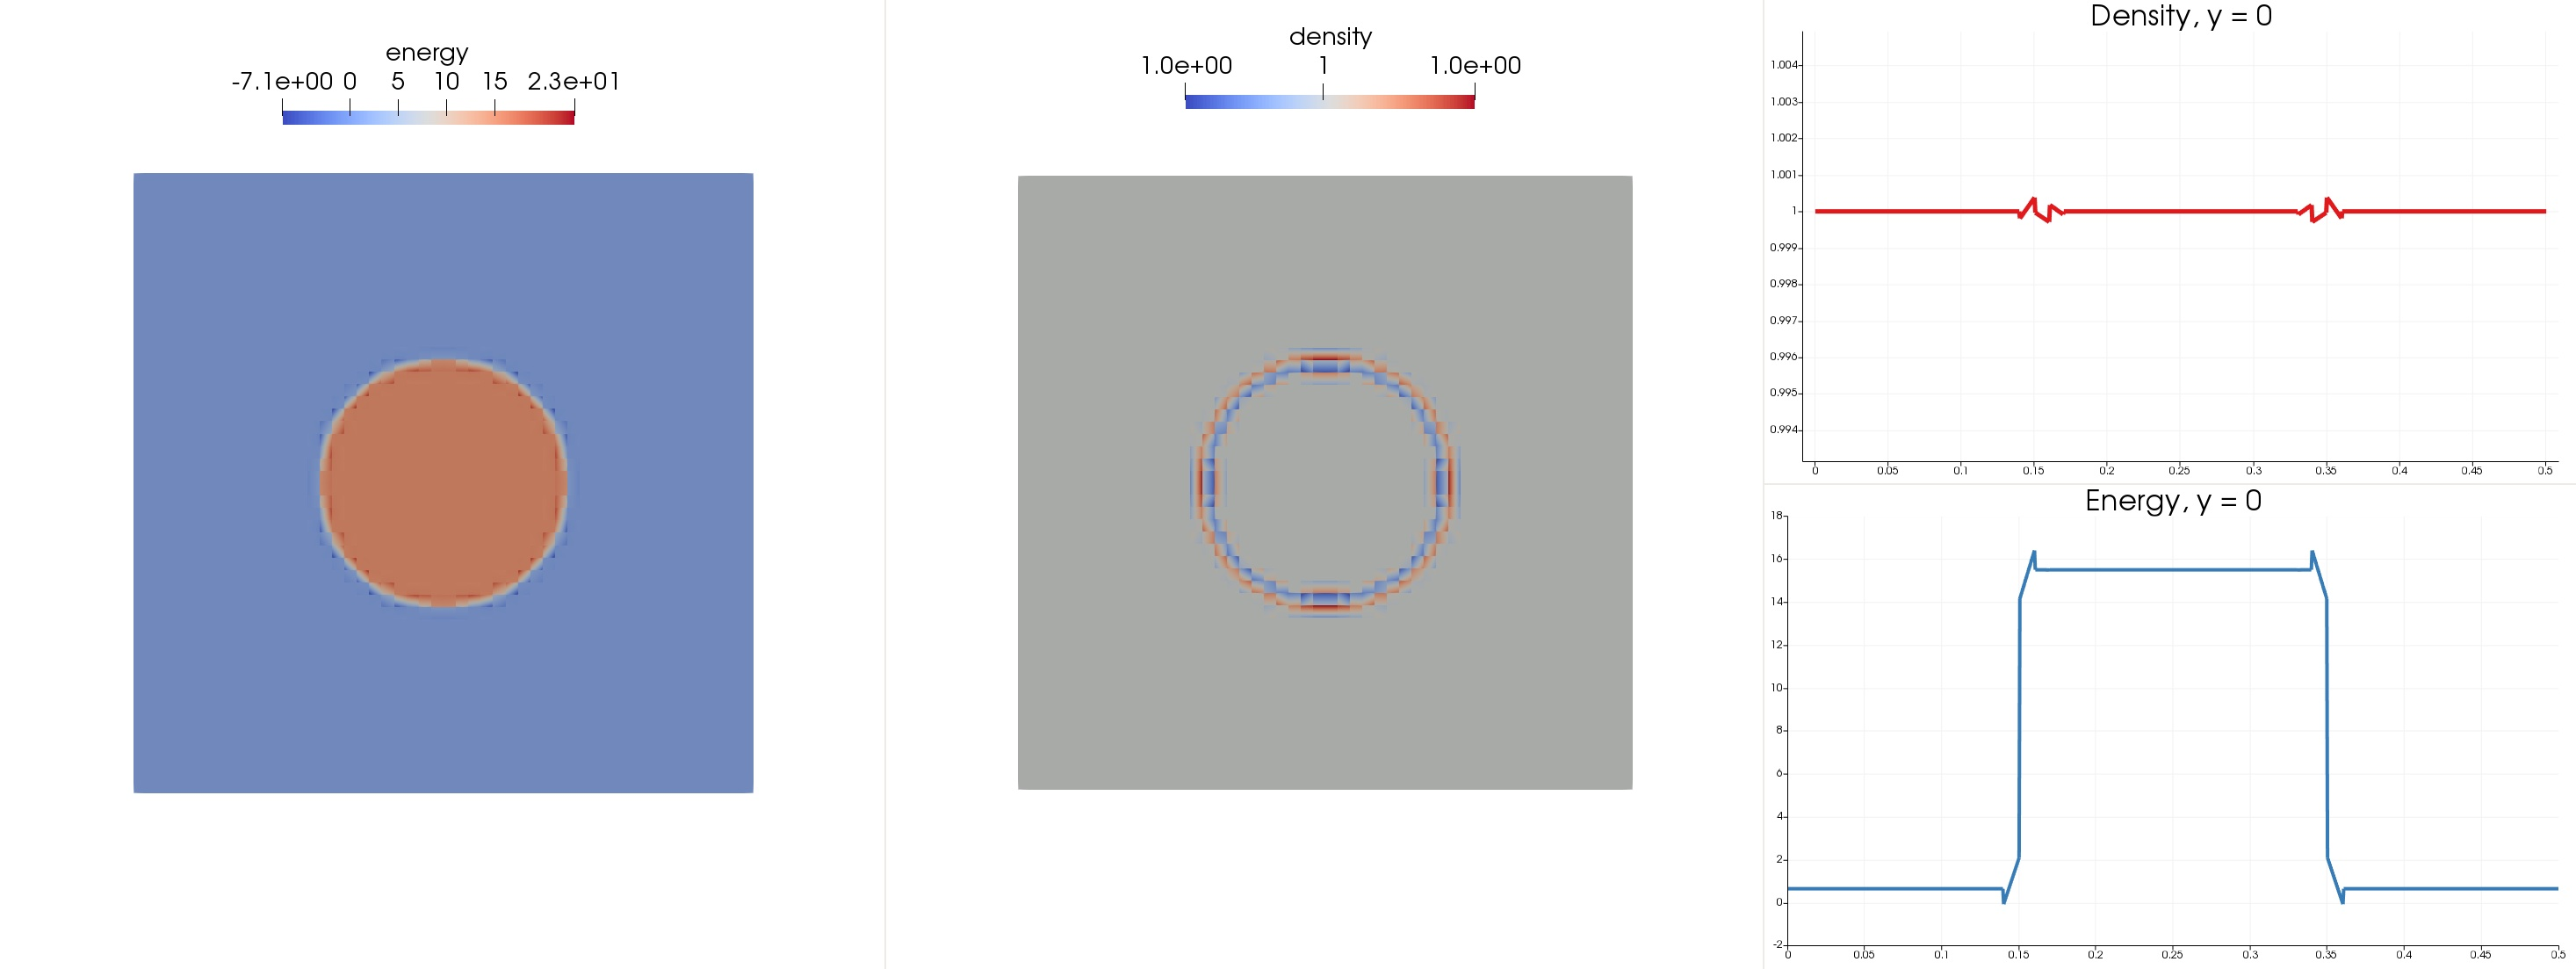
\includegraphics[width=0.82\textwidth]{img/limit/nl1.jpg}
		\end{center}
	\end{figure}\vspace{-12mm}
	\begin{figure}[H]
		\begin{center}
			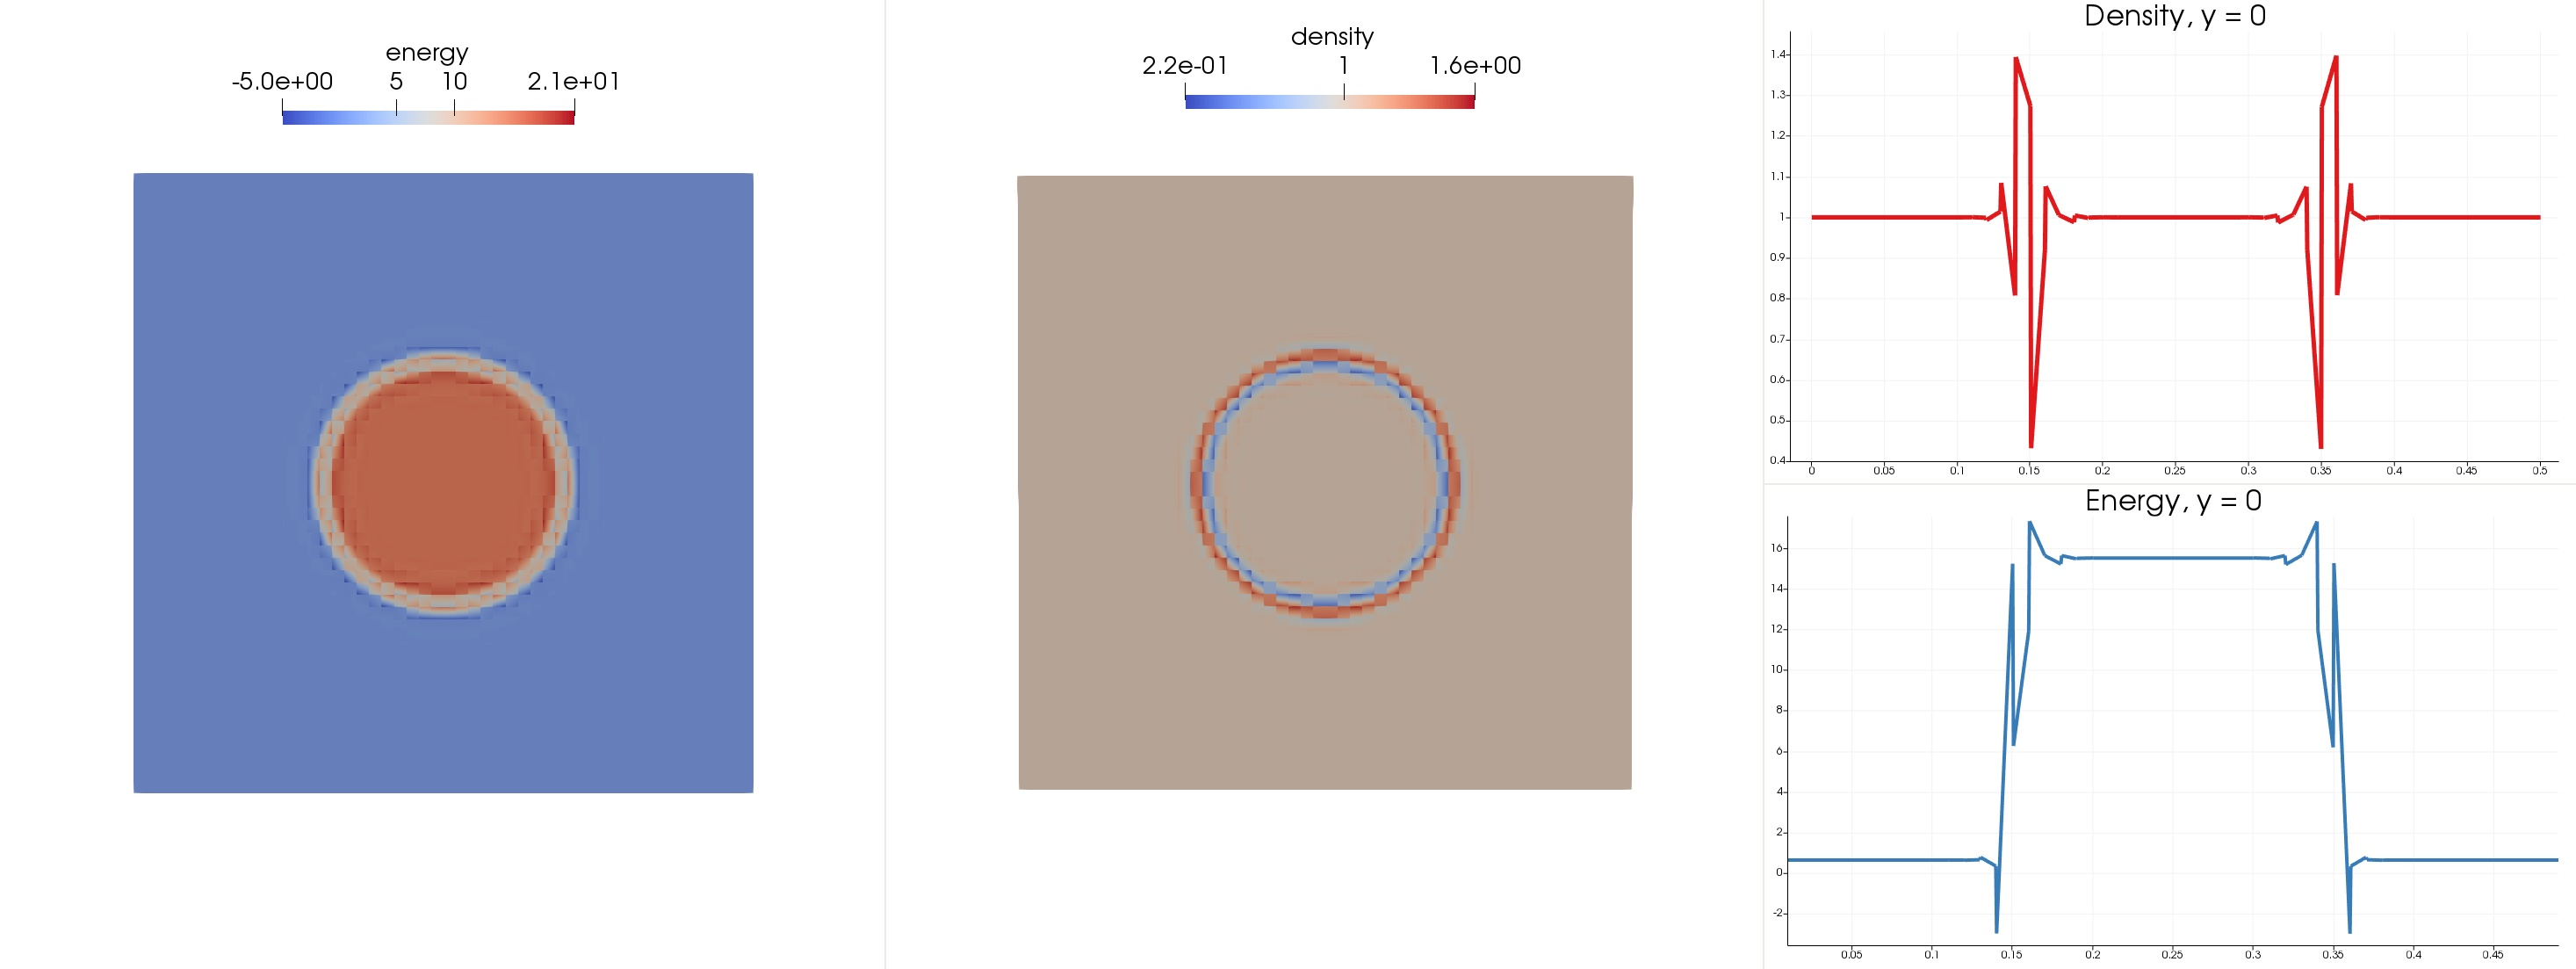
\includegraphics[width=0.82\textwidth]{img/limit/nl2.jpg}
		\end{center}
	\end{figure}\vspace{-12mm}
	\begin{figure}[H]
		\begin{center}
			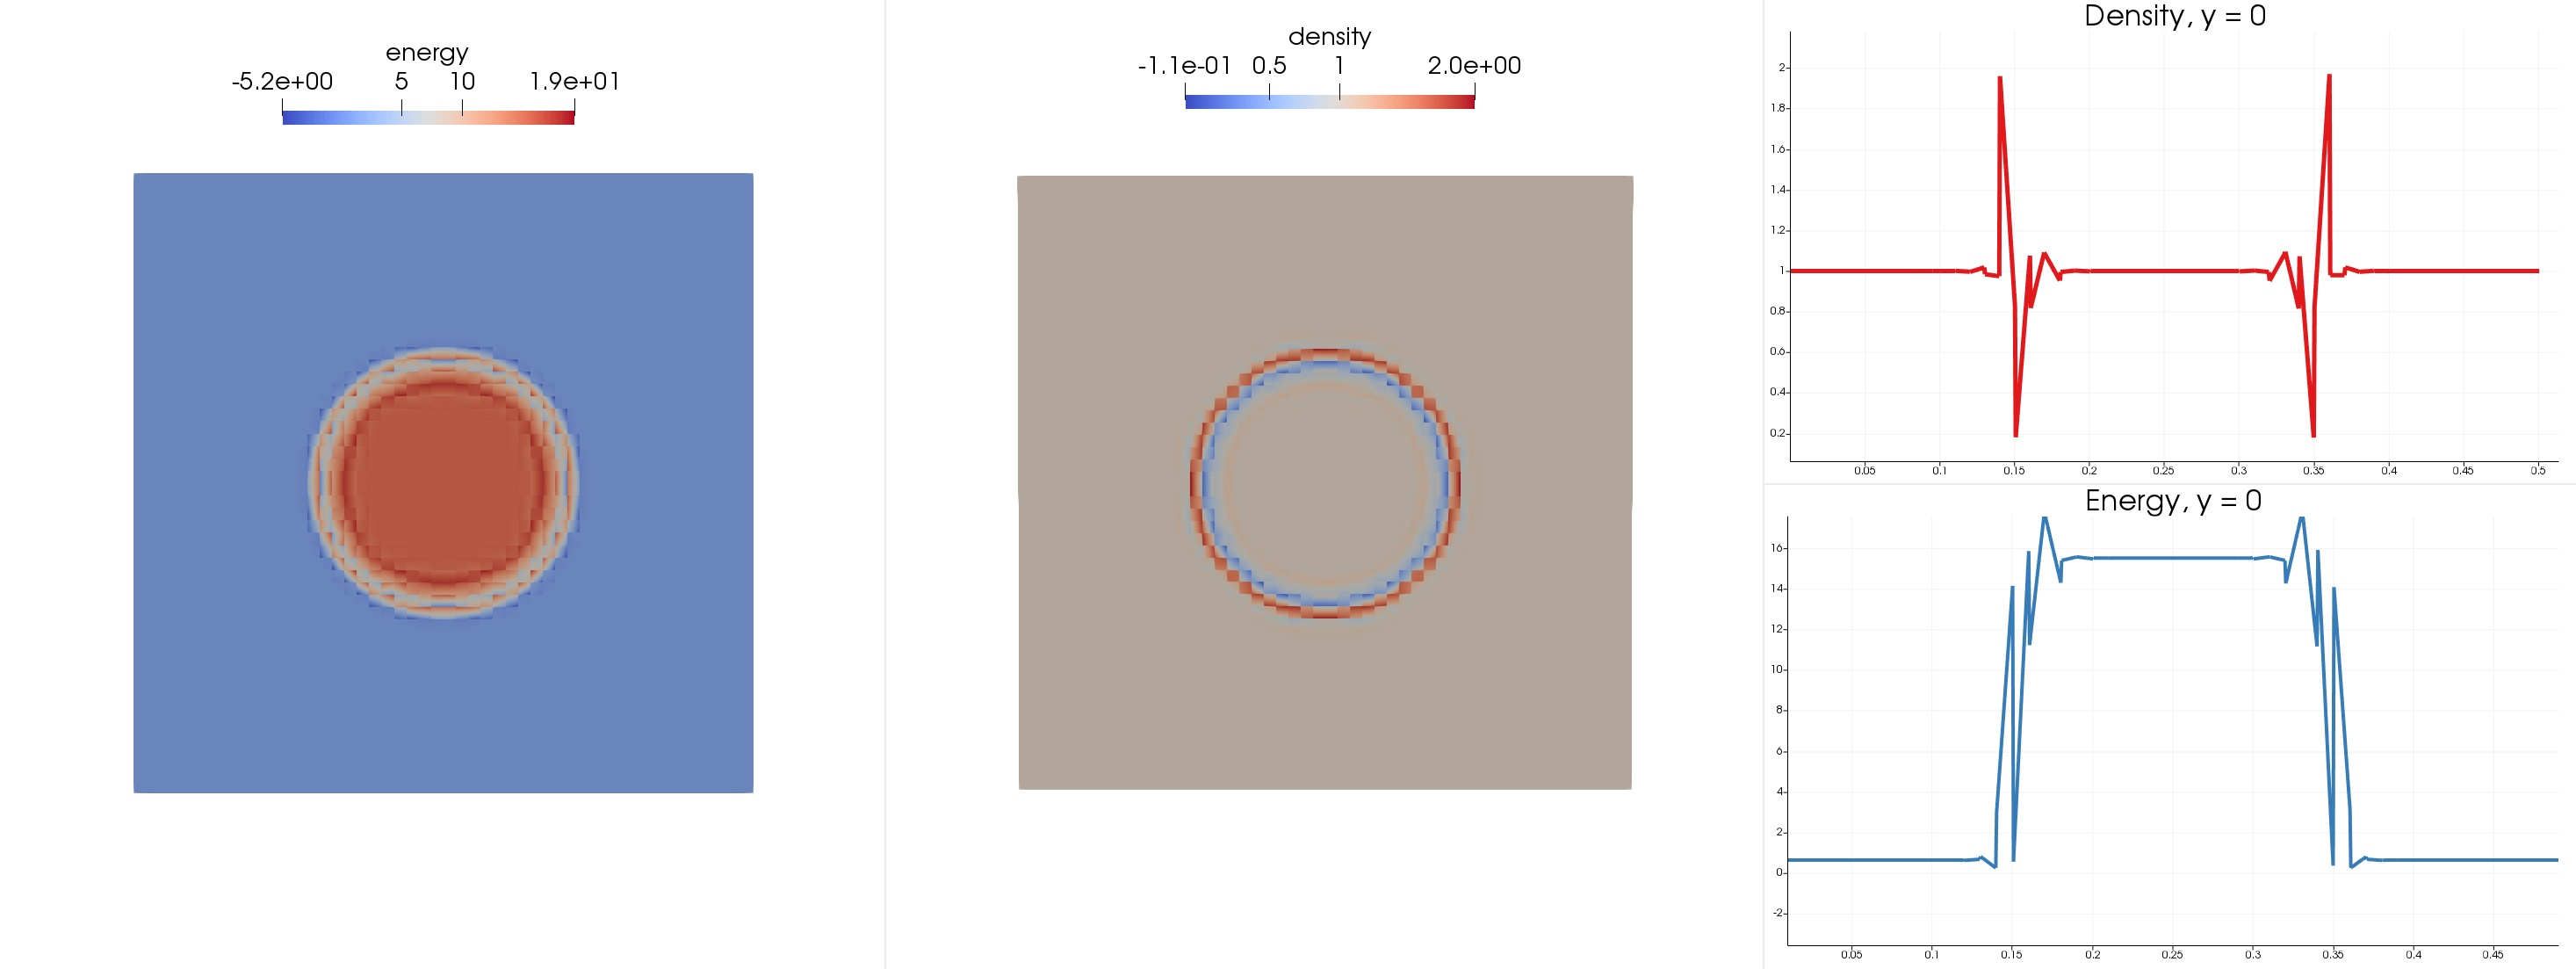
\includegraphics[width=0.82\textwidth]{img/limit/nl3.jpg}
		\end{center}
	\end{figure}\vspace{-12mm}
	\begin{figure}[H]
		\begin{center}
			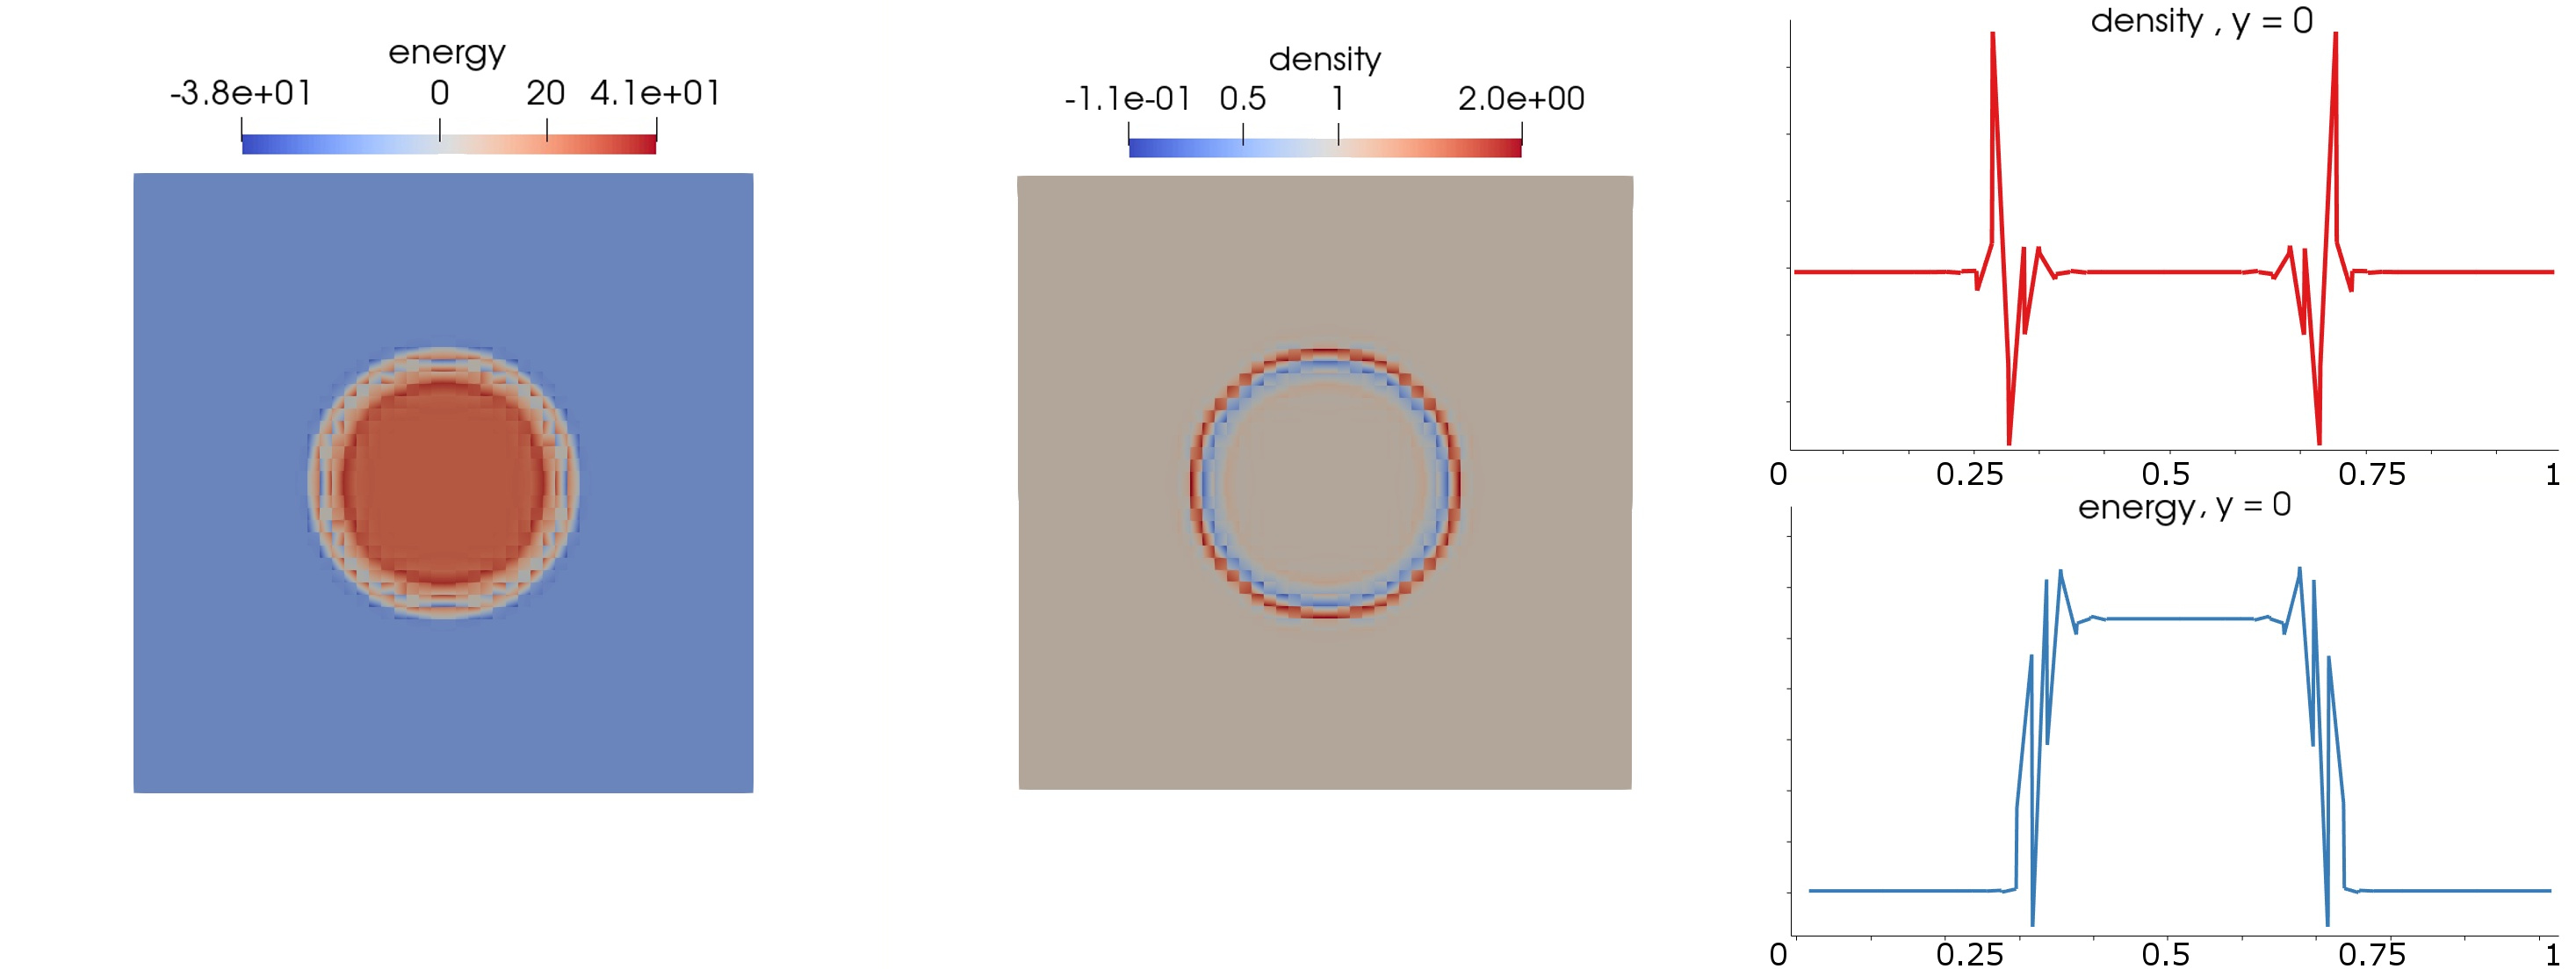
\includegraphics[width=0.82\textwidth]{img/limit/nl4.jpg}
		\end{center}
	\end{figure}\vspace{-12mm}
	\begin{figure}[H]
		\begin{center}
			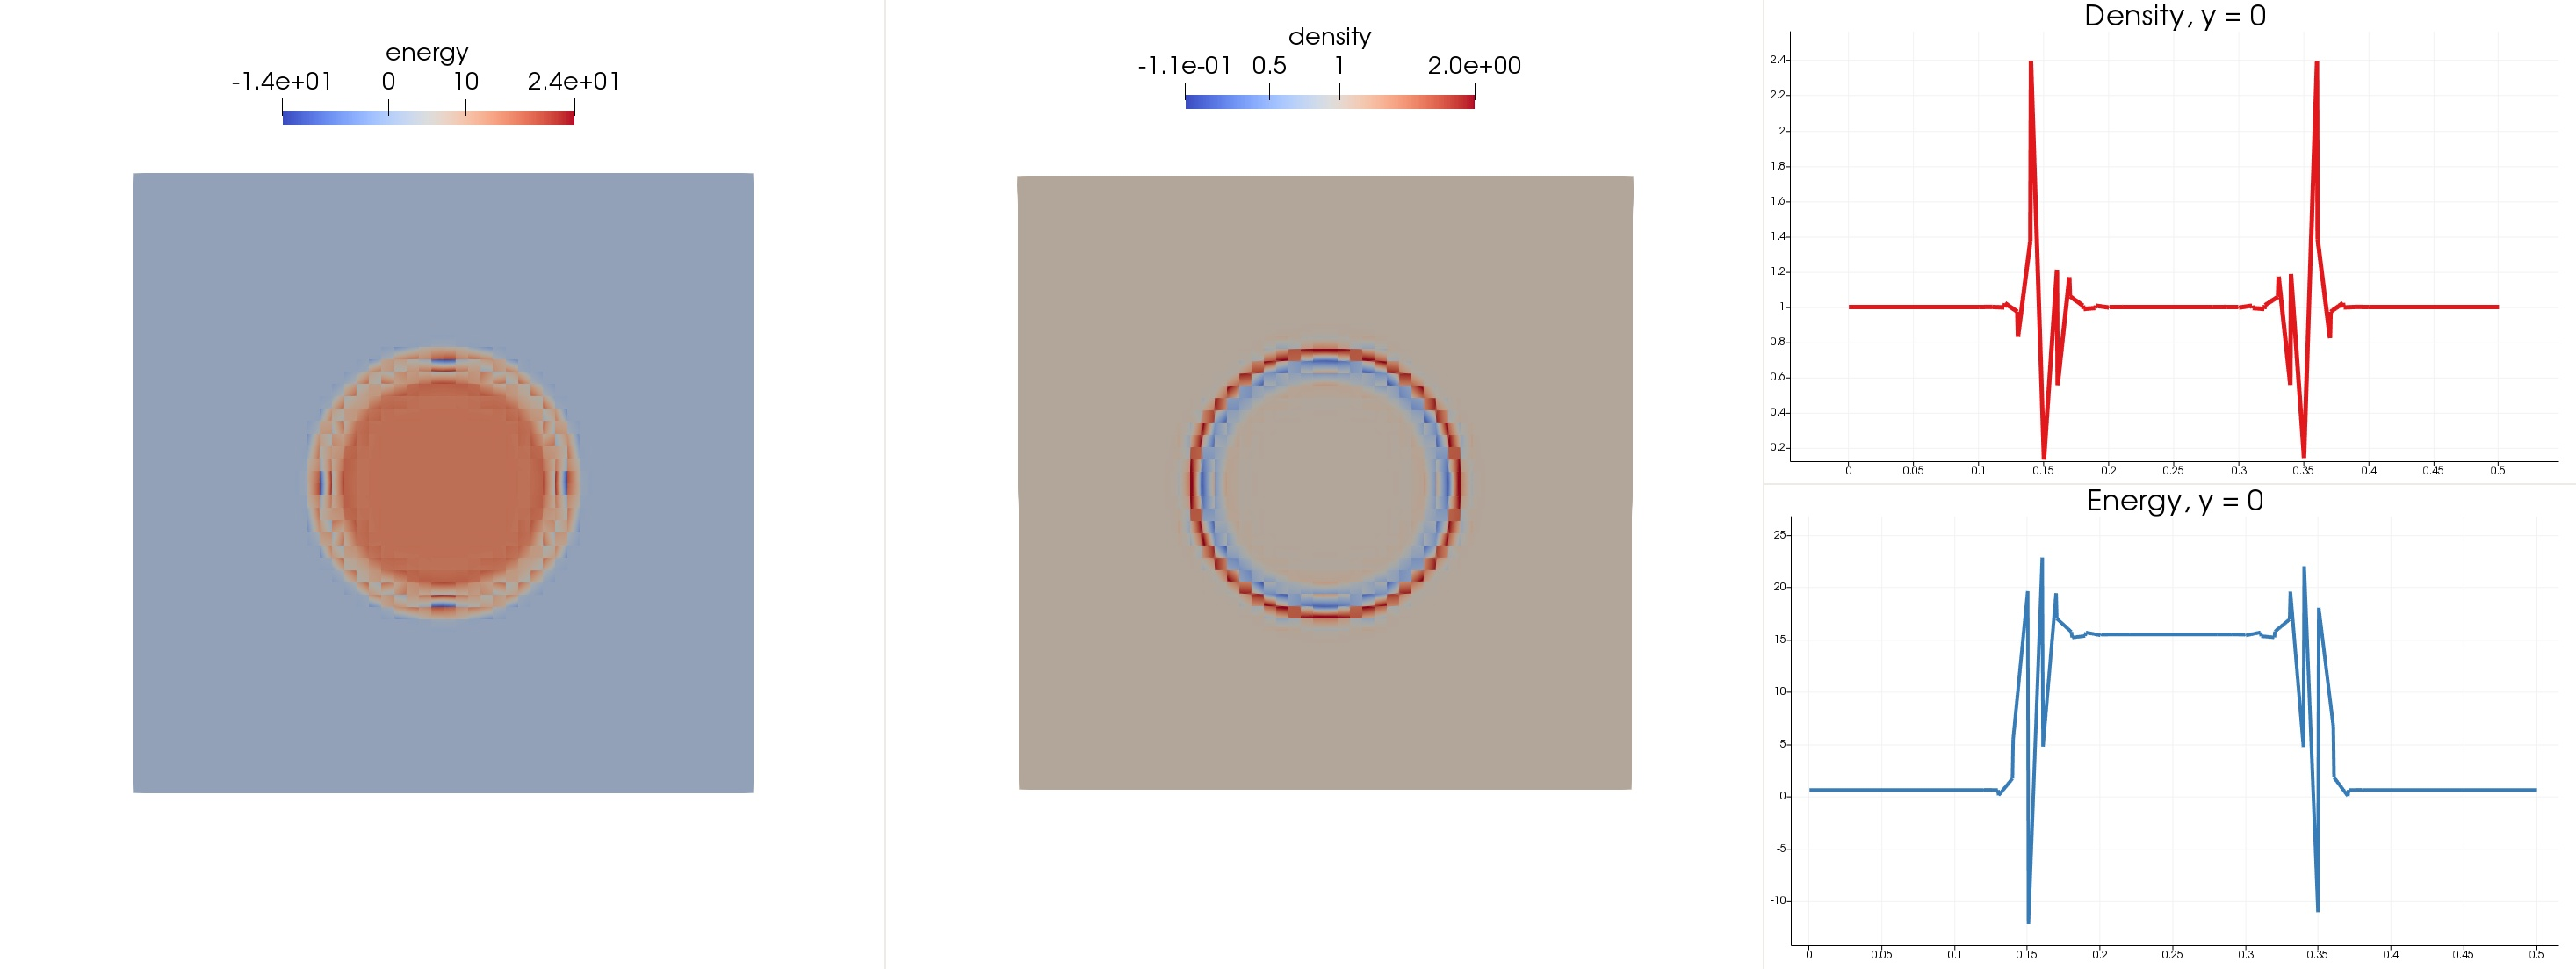
\includegraphics[width=0.82\textwidth]{img/limit/nl5.jpg}
		\end{center}
	\end{figure}\vspace{-12mm}
	\begin{figure}[H]
		\begin{center}
			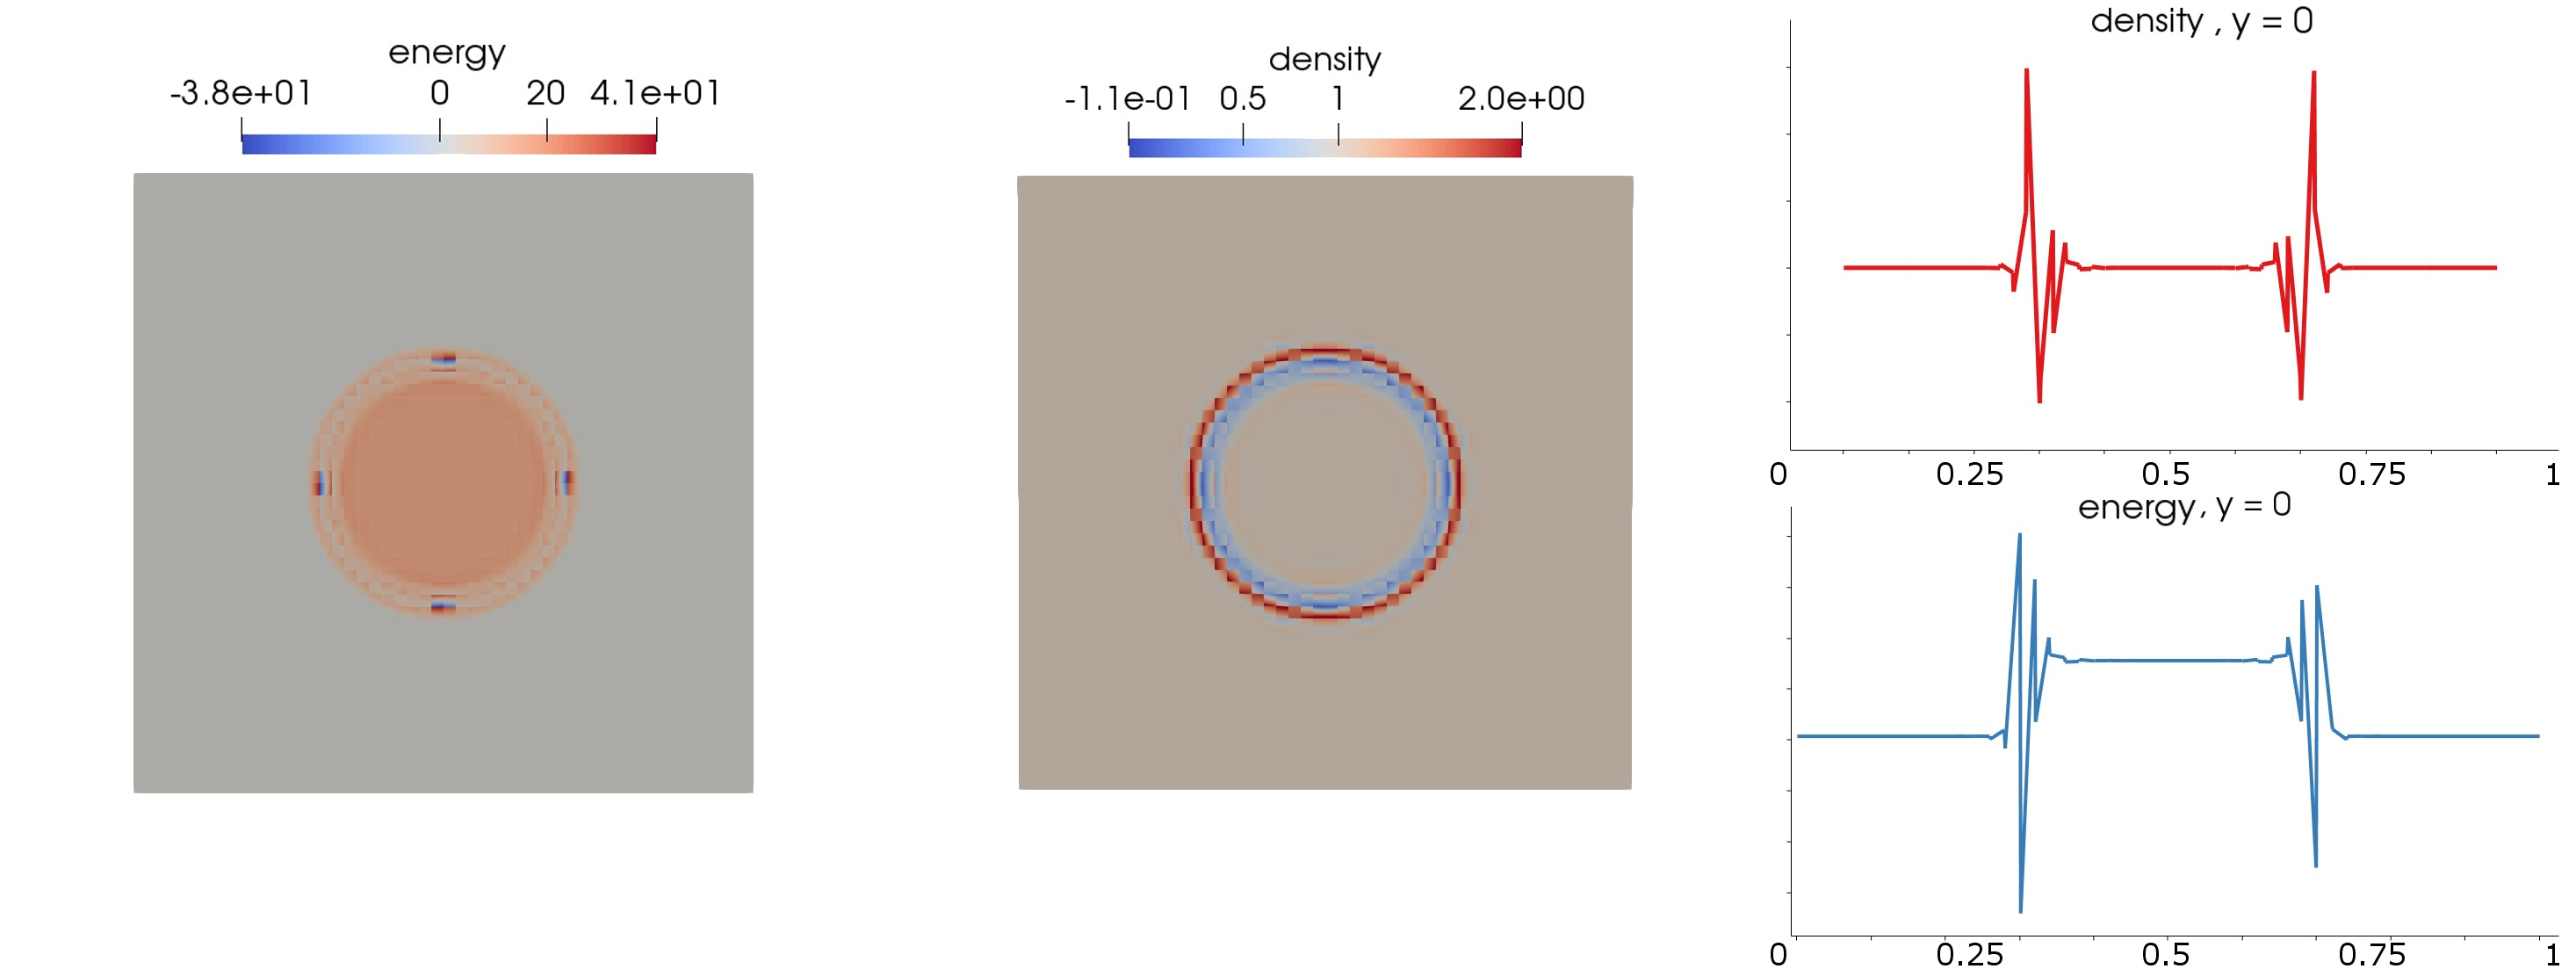
\includegraphics[width=0.82\textwidth]{img/limit/nl6.jpg}		
			\vspace{-4mm}
			\caption{Unlimited solution - Energy, density, and their values over line y = 0, the solution cannot progress beyond the last snapshot, as the oscillations are orders of magnitude larger than the physical solution}
		\end{center}
	\end{figure}
	
	\newpage
	
\begin{figure}[H]
		\begin{center}
			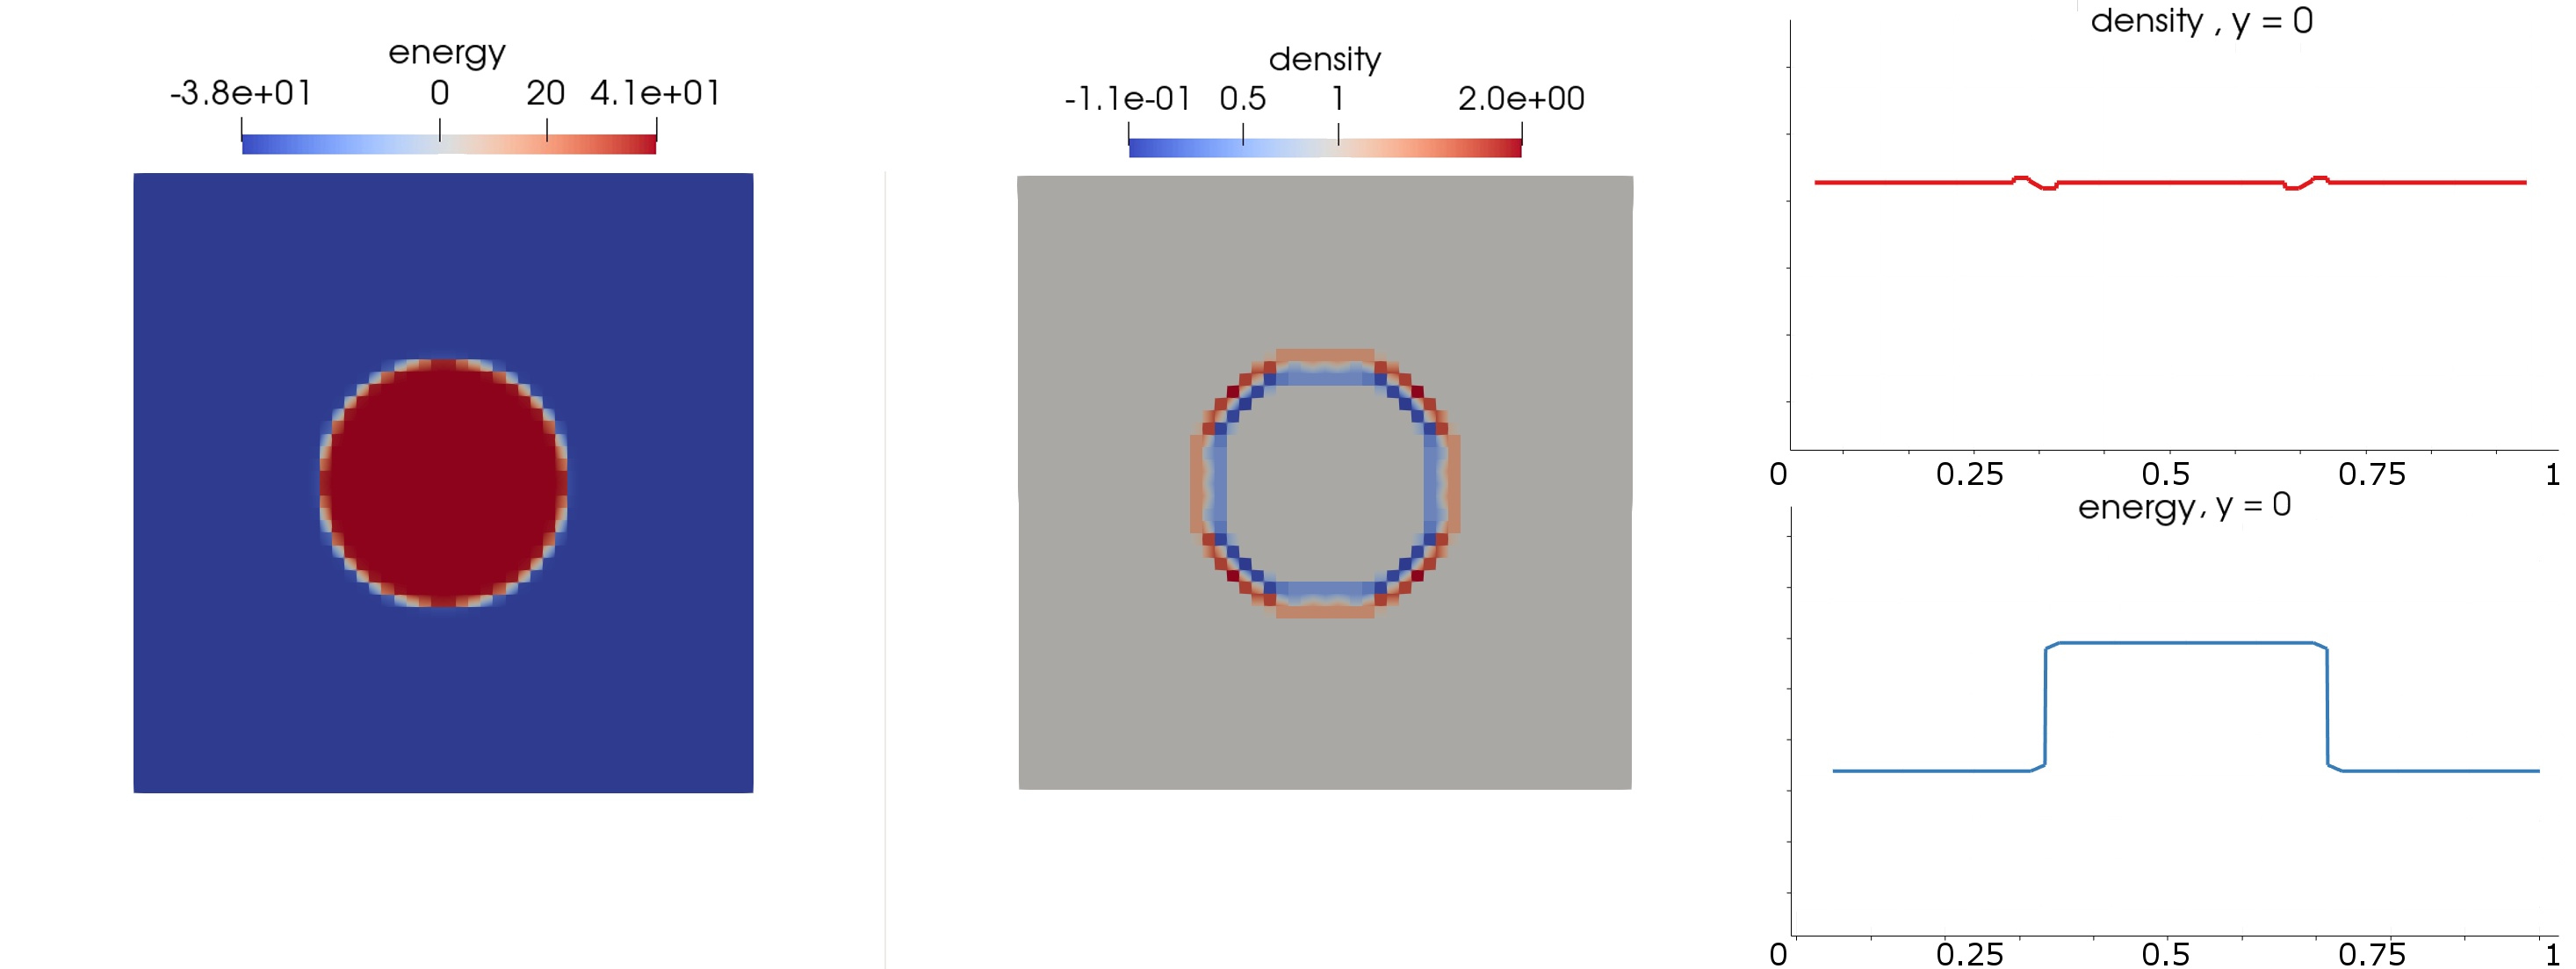
\includegraphics[width=0.82\textwidth]{img/limit/l1.jpg}
		\end{center}
	\end{figure}\vspace{-12mm}
	\begin{figure}[H]
		\begin{center}
			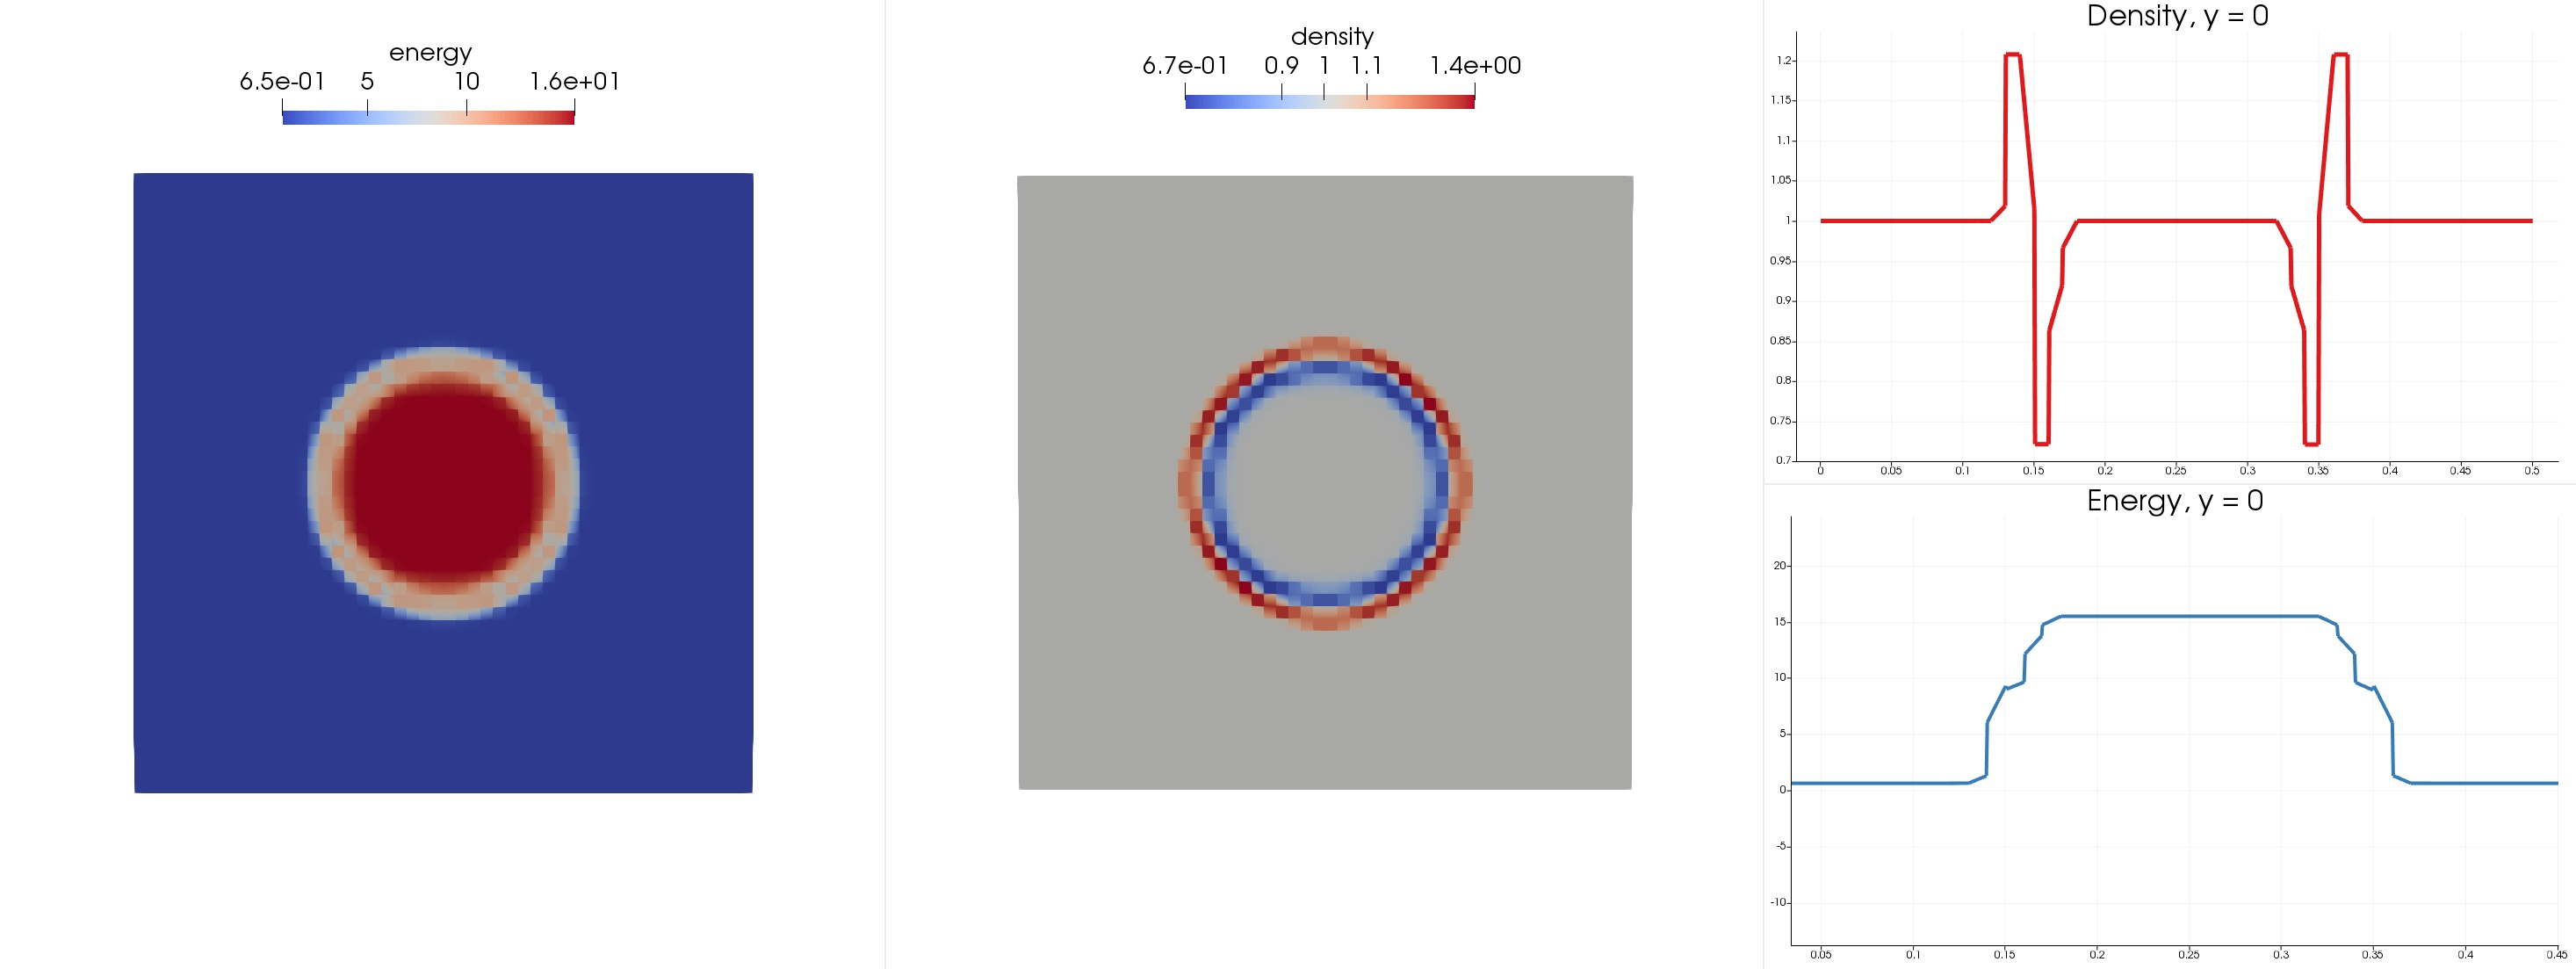
\includegraphics[width=0.82\textwidth]{img/limit/l2.jpg}
		\end{center}
	\end{figure}\vspace{-12mm}
	\begin{figure}[H]
		\begin{center}
			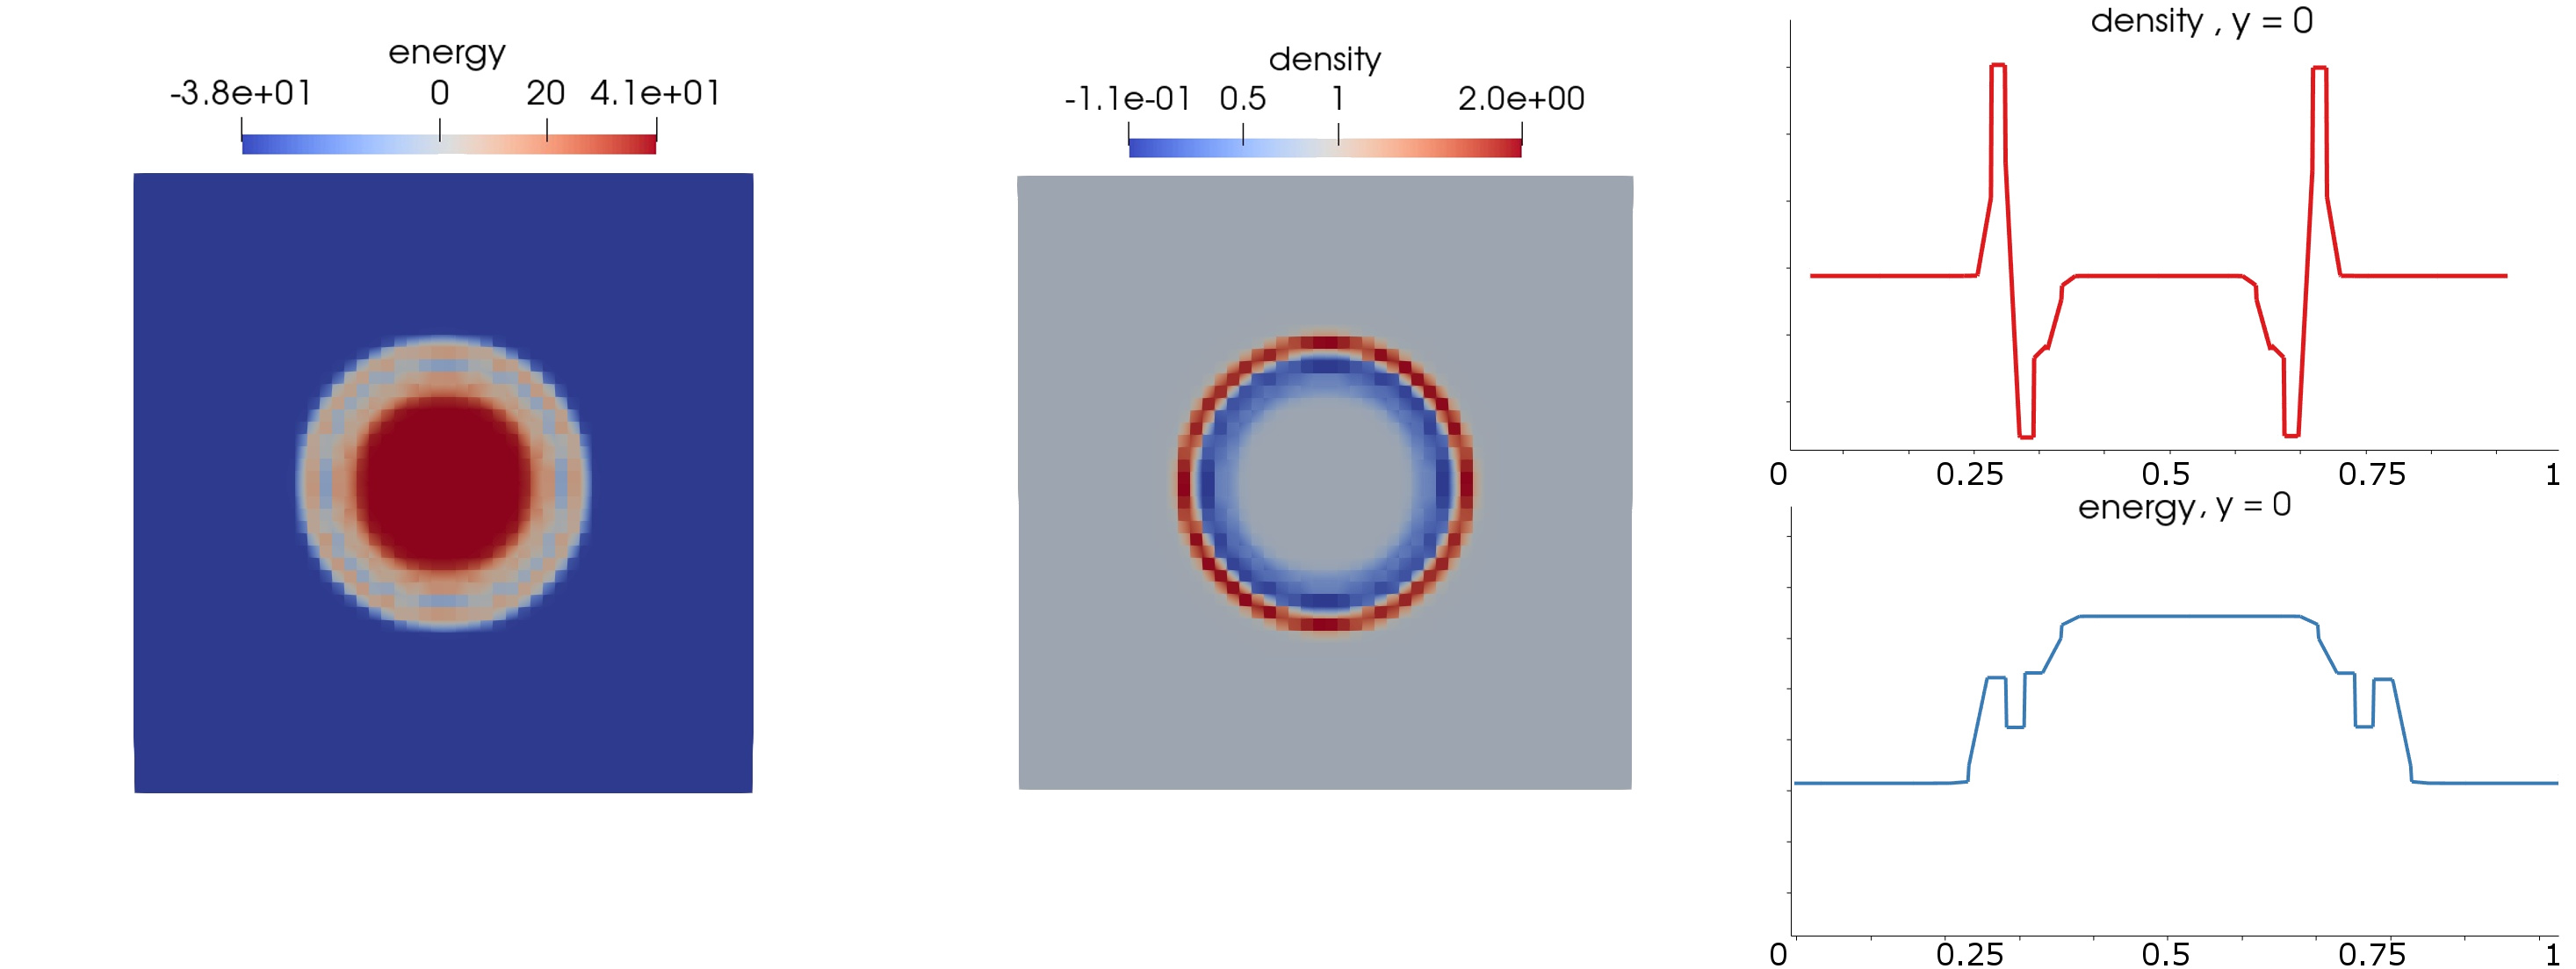
\includegraphics[width=0.82\textwidth]{img/limit/l3.jpg}
		\end{center}
	\end{figure}\vspace{-12mm}
	\begin{figure}[H]
		\begin{center}
			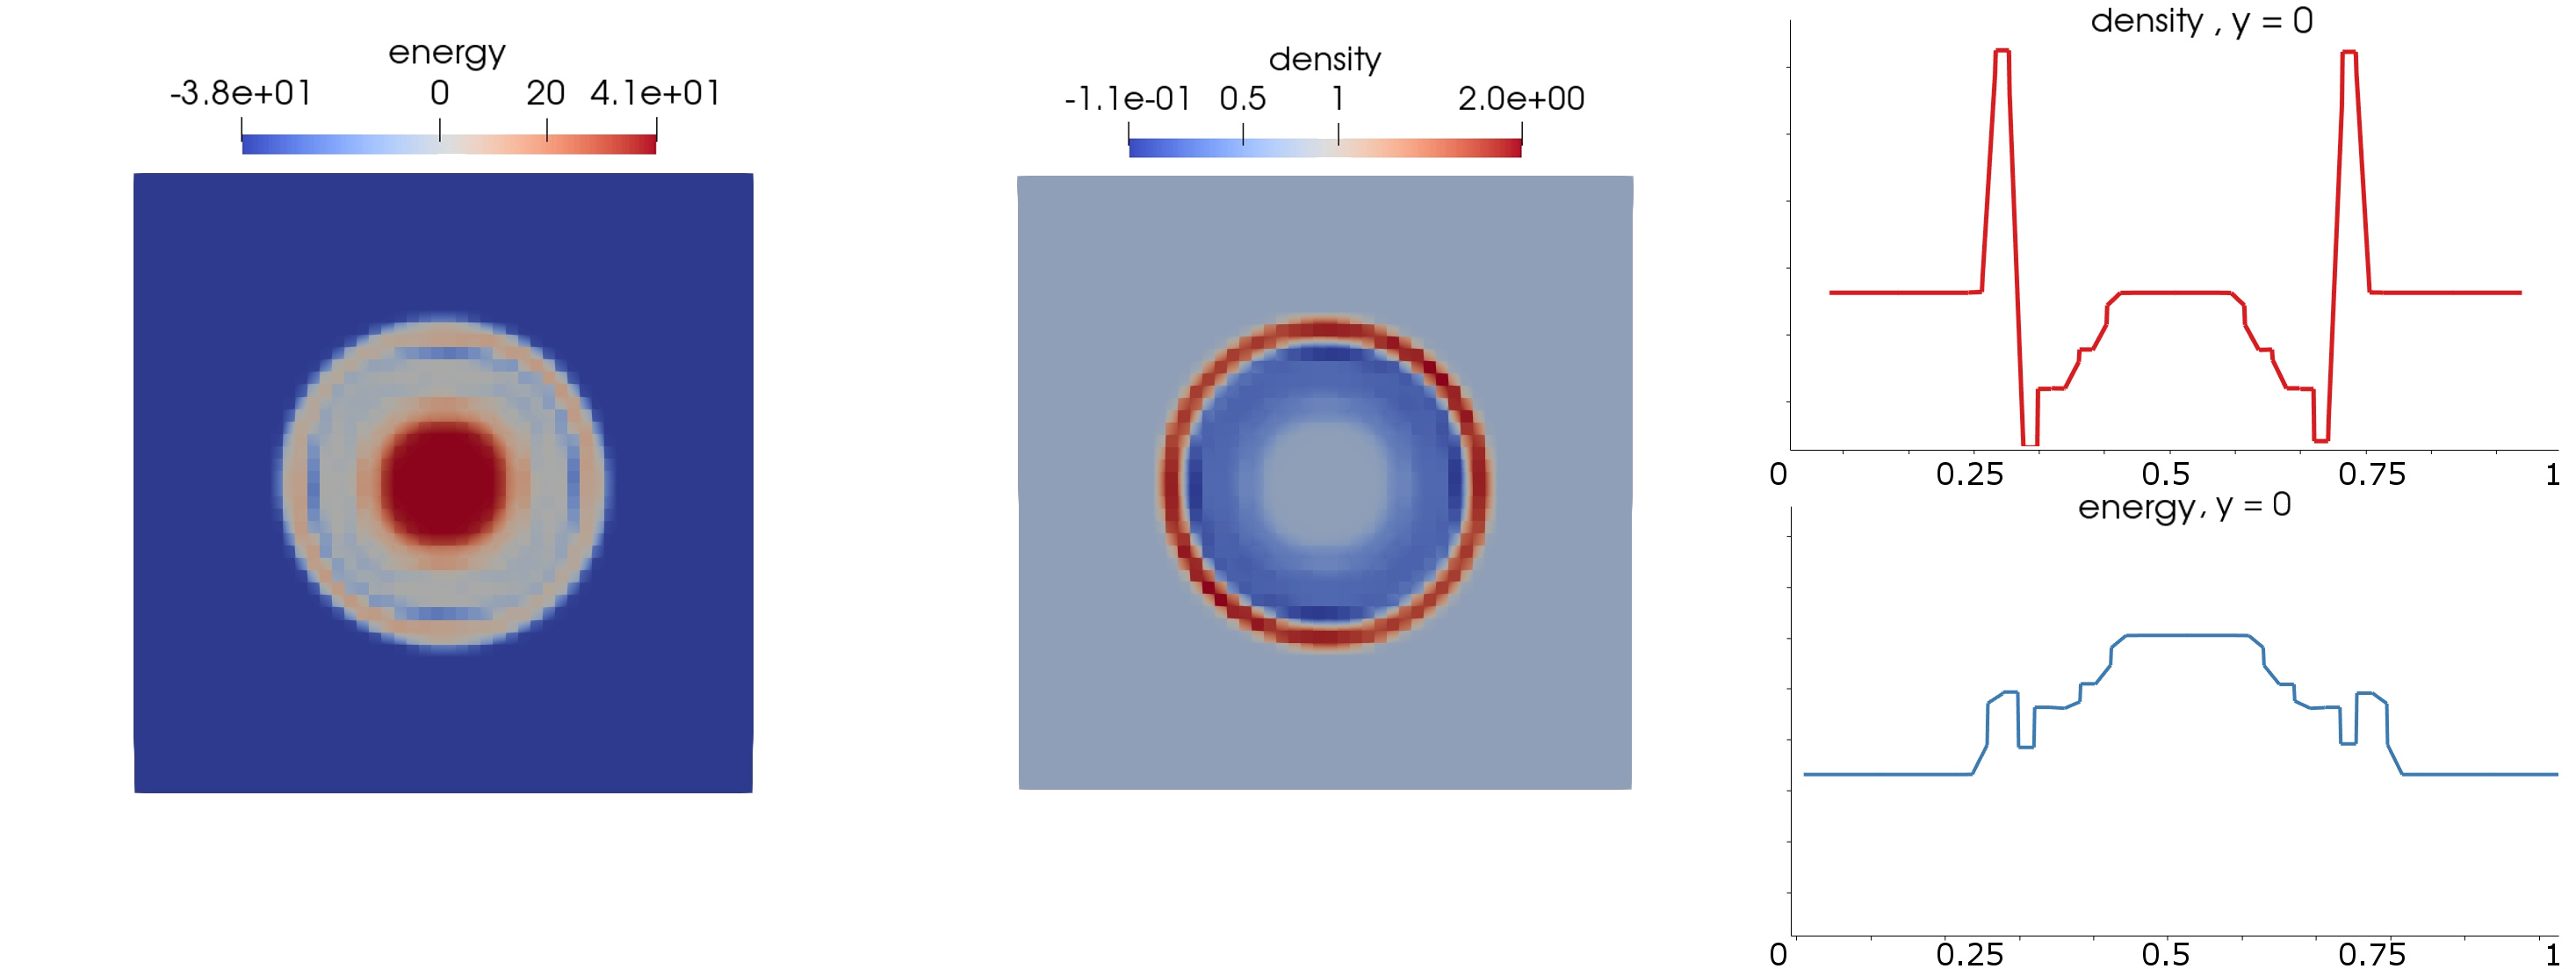
\includegraphics[width=0.82\textwidth]{img/limit/l4.jpg}
		\end{center}
	\end{figure}\vspace{-12mm}
	\begin{figure}[H]
		\begin{center}
			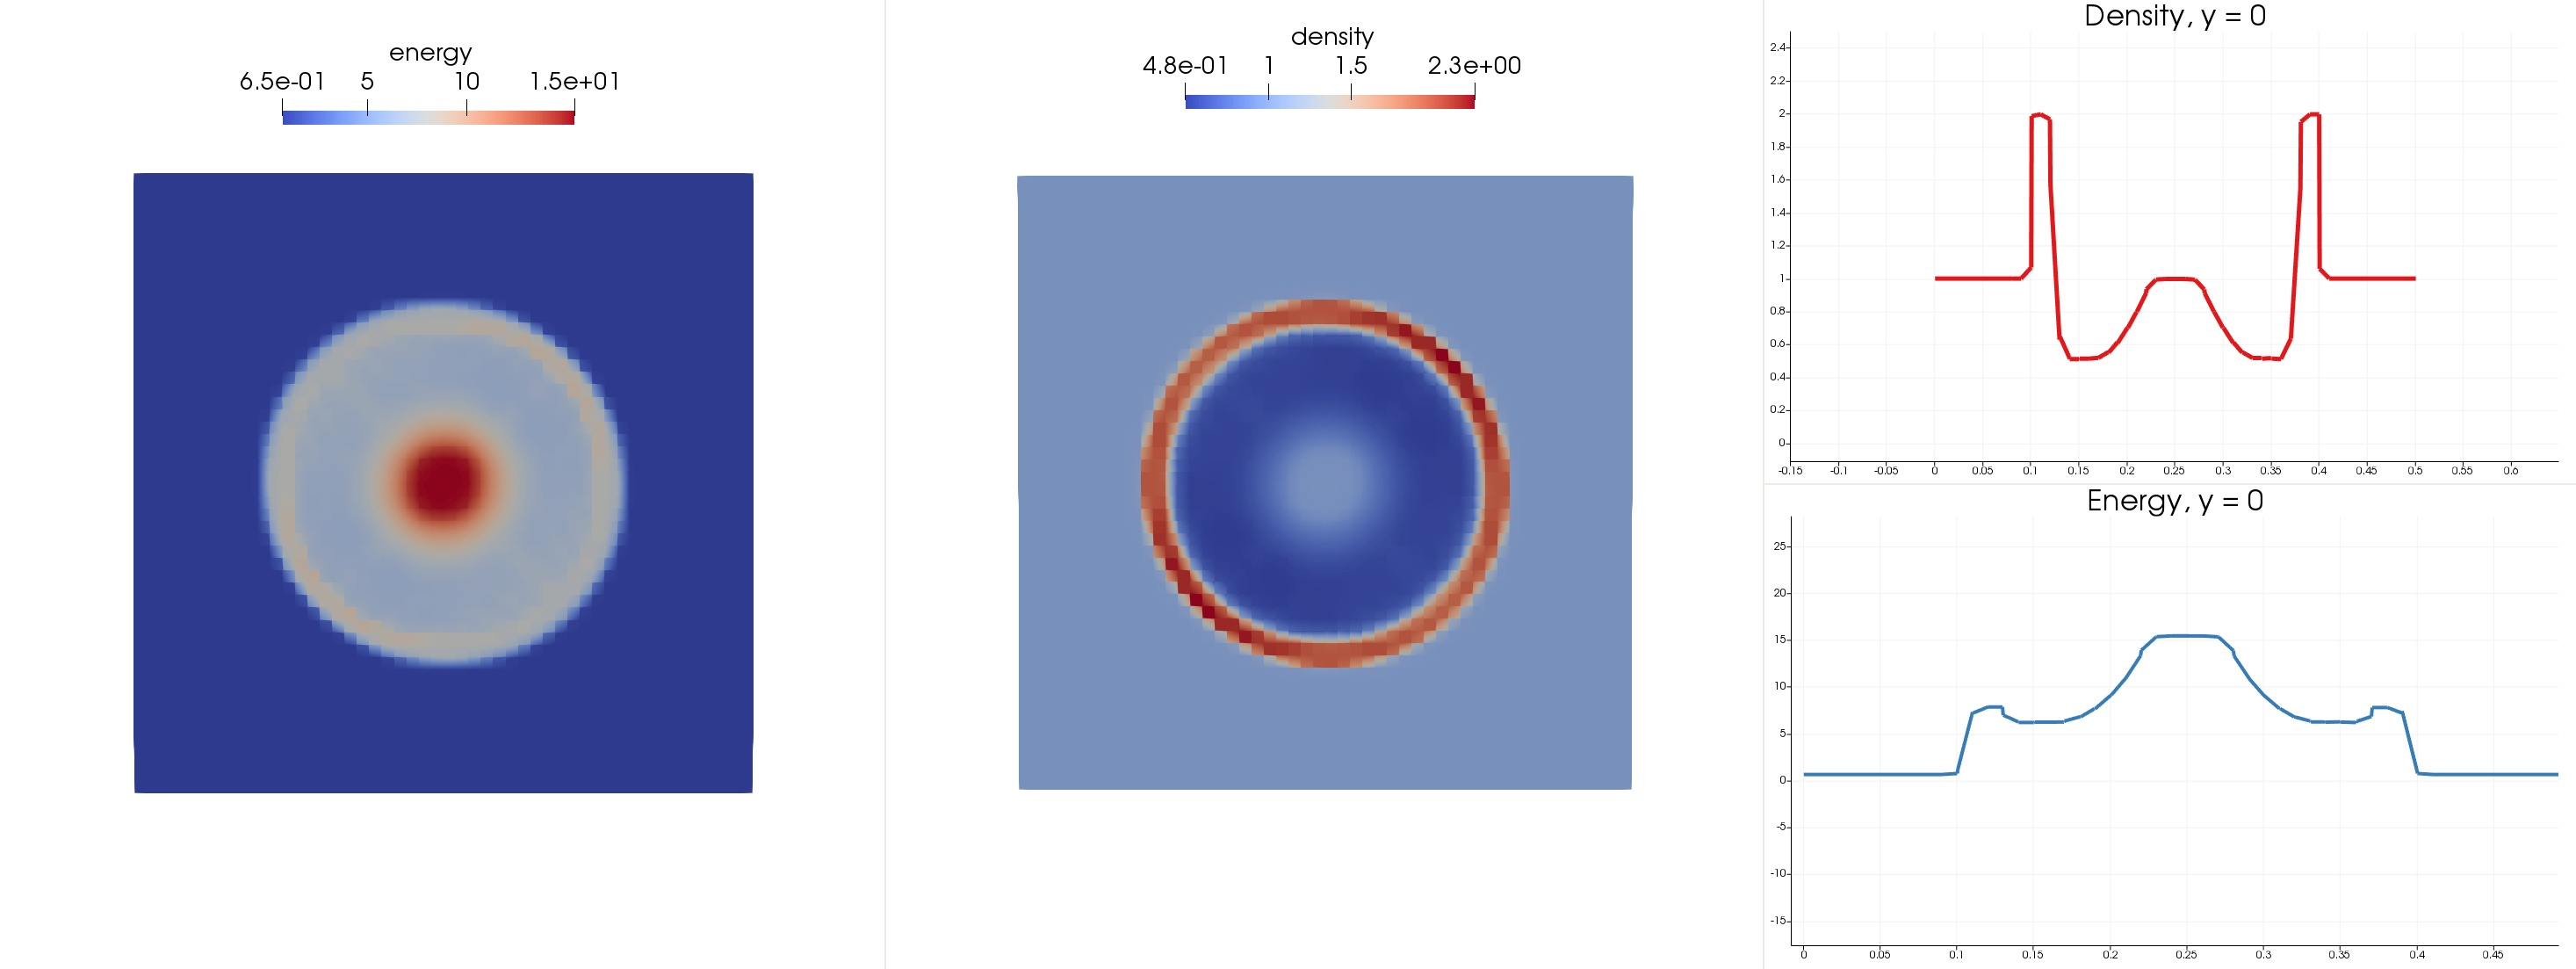
\includegraphics[width=0.82\textwidth]{img/limit/l5.jpg}
		\end{center}
	\end{figure}\vspace{-12mm}
	\begin{figure}[H]
		\begin{center}
			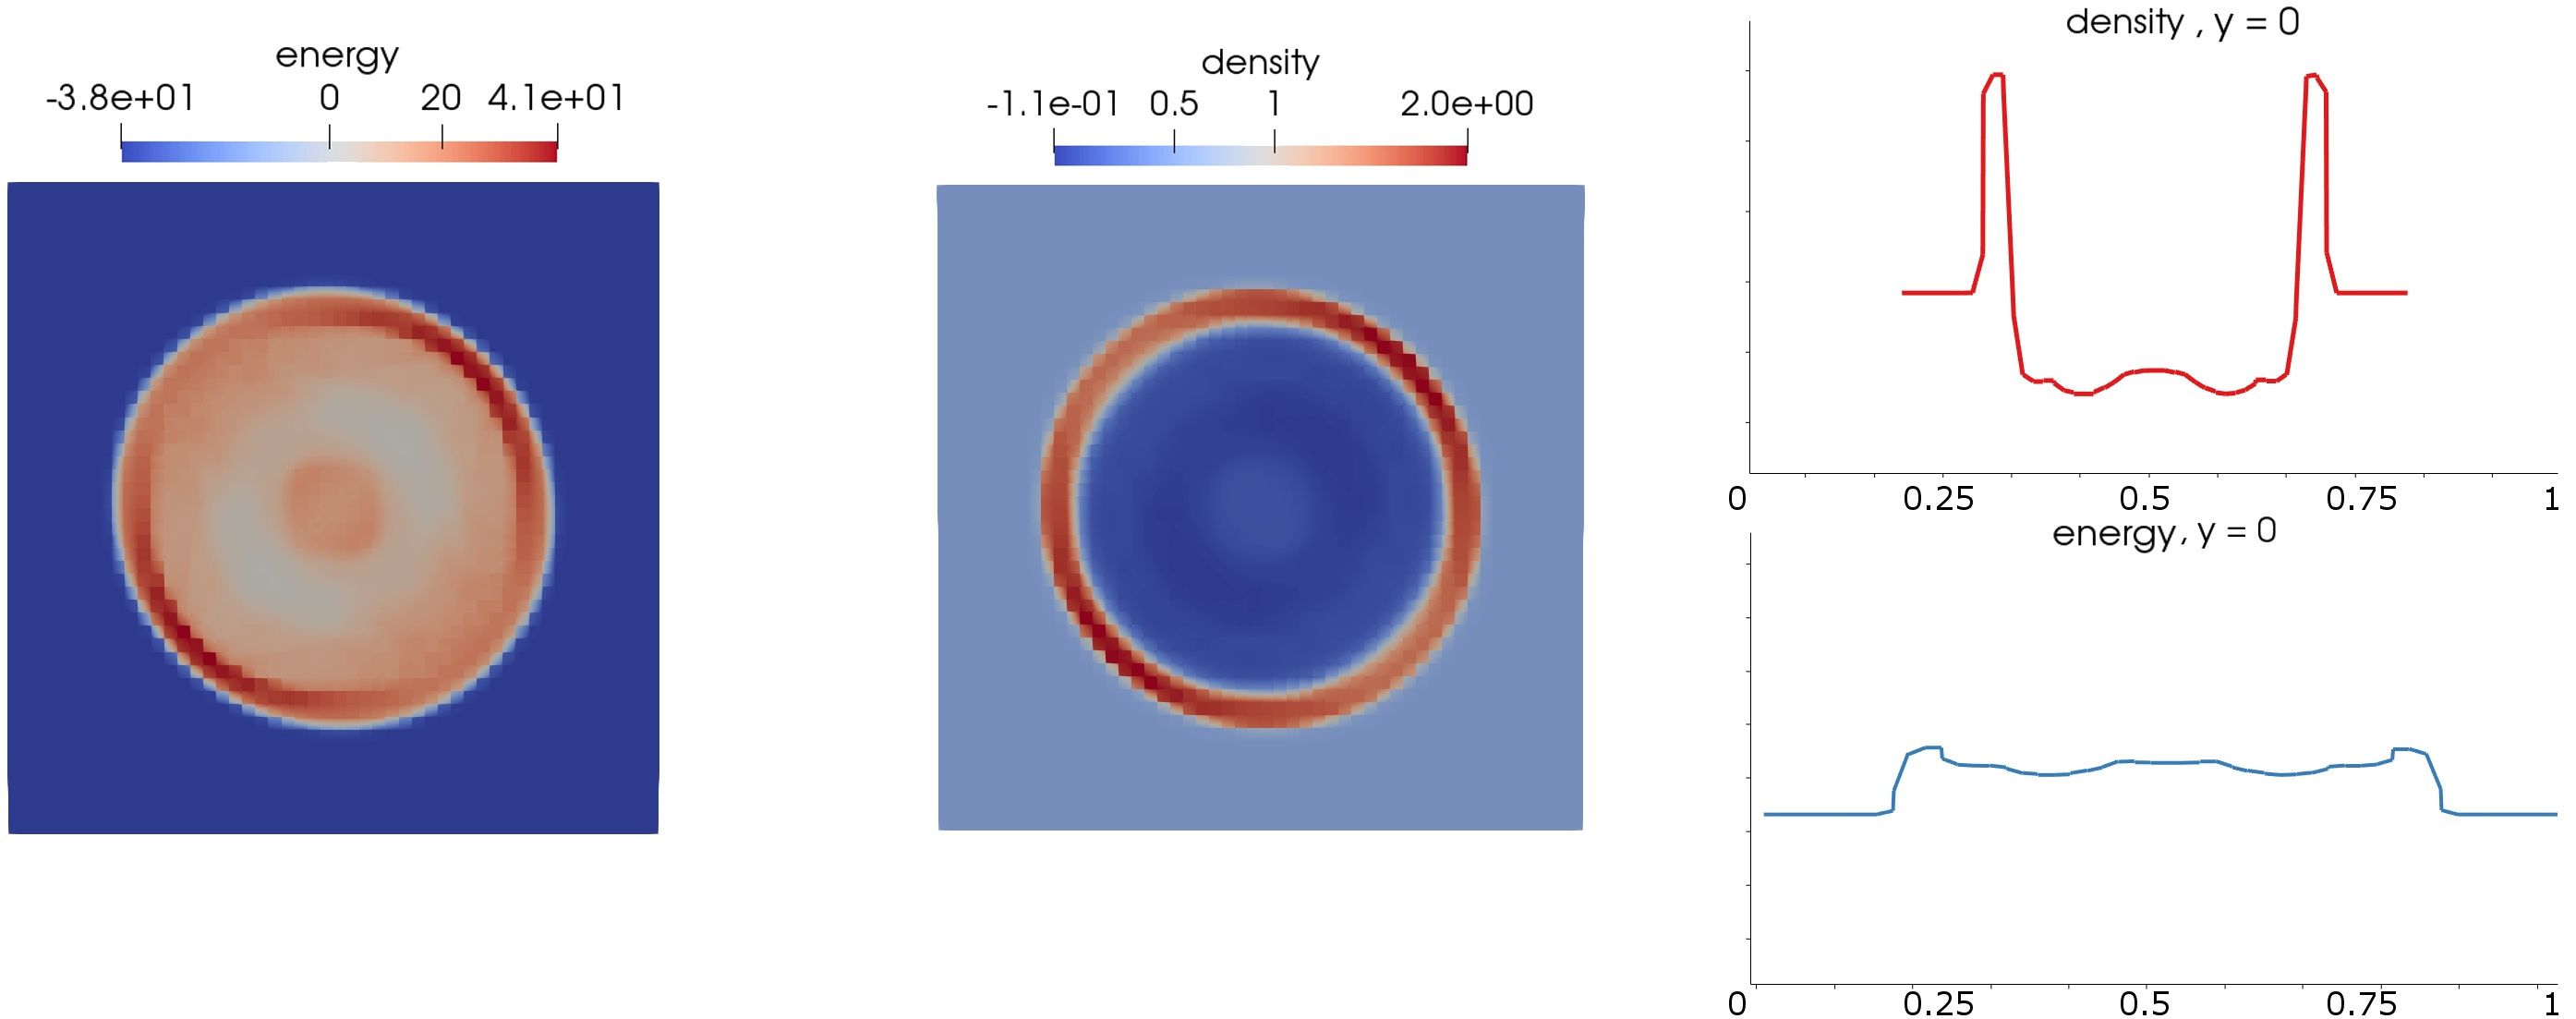
\includegraphics[width=0.82\textwidth]{img/limit/l6.jpg}
			\vspace{-4mm}
			\caption{Solution limited with Vertex-based limiter - Energy, density, and their values over line y = 0}
		\end{center}
	\end{figure}


\section{Divergence-free FE space}
The divergence-free constraint of the magnetic field, $\bfB = 0$ (Gauss's law) is not enforced by the solution definition \ref{weakSlnDef}. Therefore, we need to perform additional work to be sure that we do not have a non-physical solution in the sense that the constraint is not satisfied.
\paragraph{}
There are two often used approaches to handle this problem - the Constraint-Transport (CT) method, and divergence cleaning. The first one is not suitable for this work, as it constraints the triangulation in such a way, that implementing Adaptive Mesh Refinement would be very complicated, if possible at all. The second approach, the divergence cleaning methods need additional postprocessing step which may be omitted for the sake of calculation efficiency. The approach taken in this work is to replace the standard FE space  \ref{feSpaceDef} with basis functions \ref{feSpaceBasis} for the magnetic field part ($B$) with a vector-valued (3-dimensional) space $V_h^B$ of functions that have exactly
\be
\nabla \cdot \mrvh^B = 0,\ \ \mrvh^B\in V_h^B,
\ee
where these functions are as before discontinuous on interfaces $\Gamma_{ij}$.
The basis of space $V_h^B$ for piecewise-linear functions can be selected in several ways, in this work, the following basis was selected:
\begin{table}[H]
	\begin{tabular*}{\textwidth}{cccc}
\hline
\\
		$\lo\begin{array}{c}B_x\lo x, y, z\ro\\B_y\lo x, y, z\ro\\B_z\lo x, y, z\ro \end{array}\ro$ & Visualization & $\lo\begin{array}{c}B_x\lo x, y, z\ro\\B_y\lo x, y, z\ro\\B_z\lo x, y, z\ro \end{array}\ro$ & Visualization \\ 
\\
		\hline
		\\
\end{tabular*}
	\begin{tabular*}{\textwidth}{cccc}
	$\lo\begin{array}{c}1\\0\\0 \end{array}\ro$ & \raisebox{-0.5\totalheight}{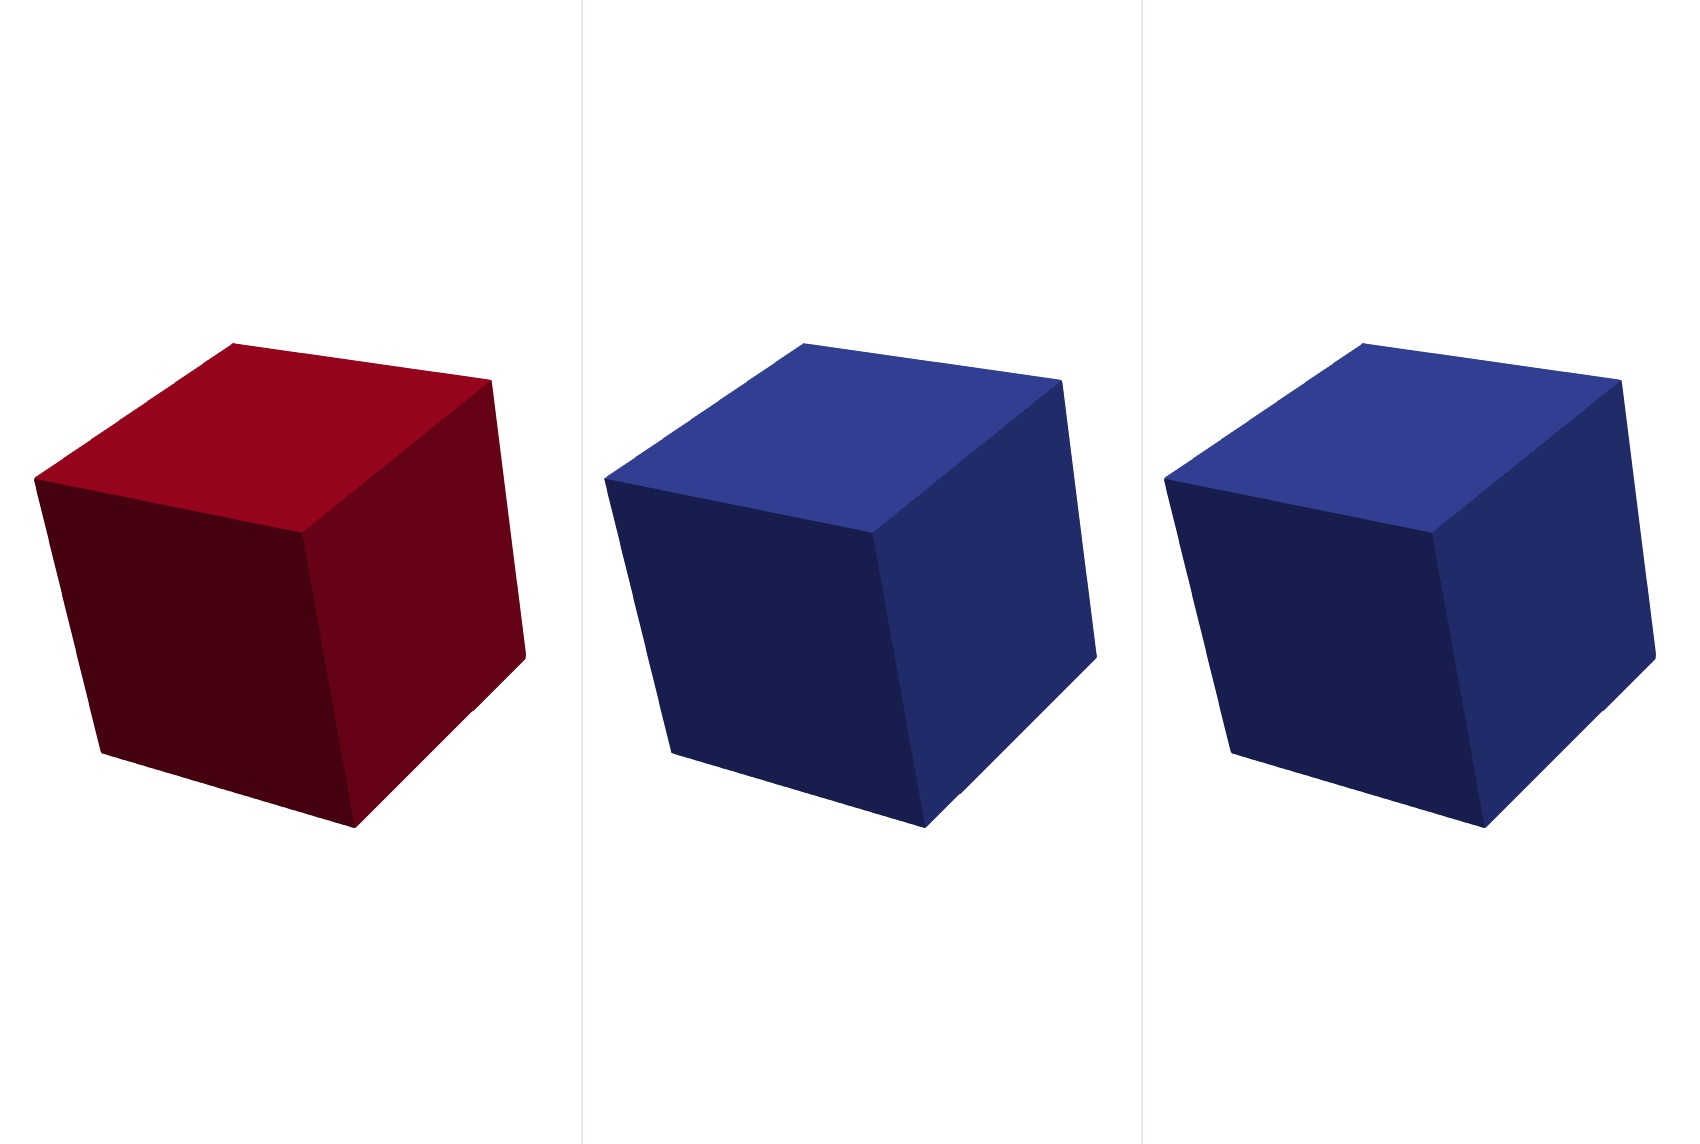
\includegraphics[width=0.3\textwidth]{img/basis/1.jpg}} & $\lo\begin{array}{c}0\\0\\y \end{array}\ro$ & \raisebox{-0.5\totalheight}{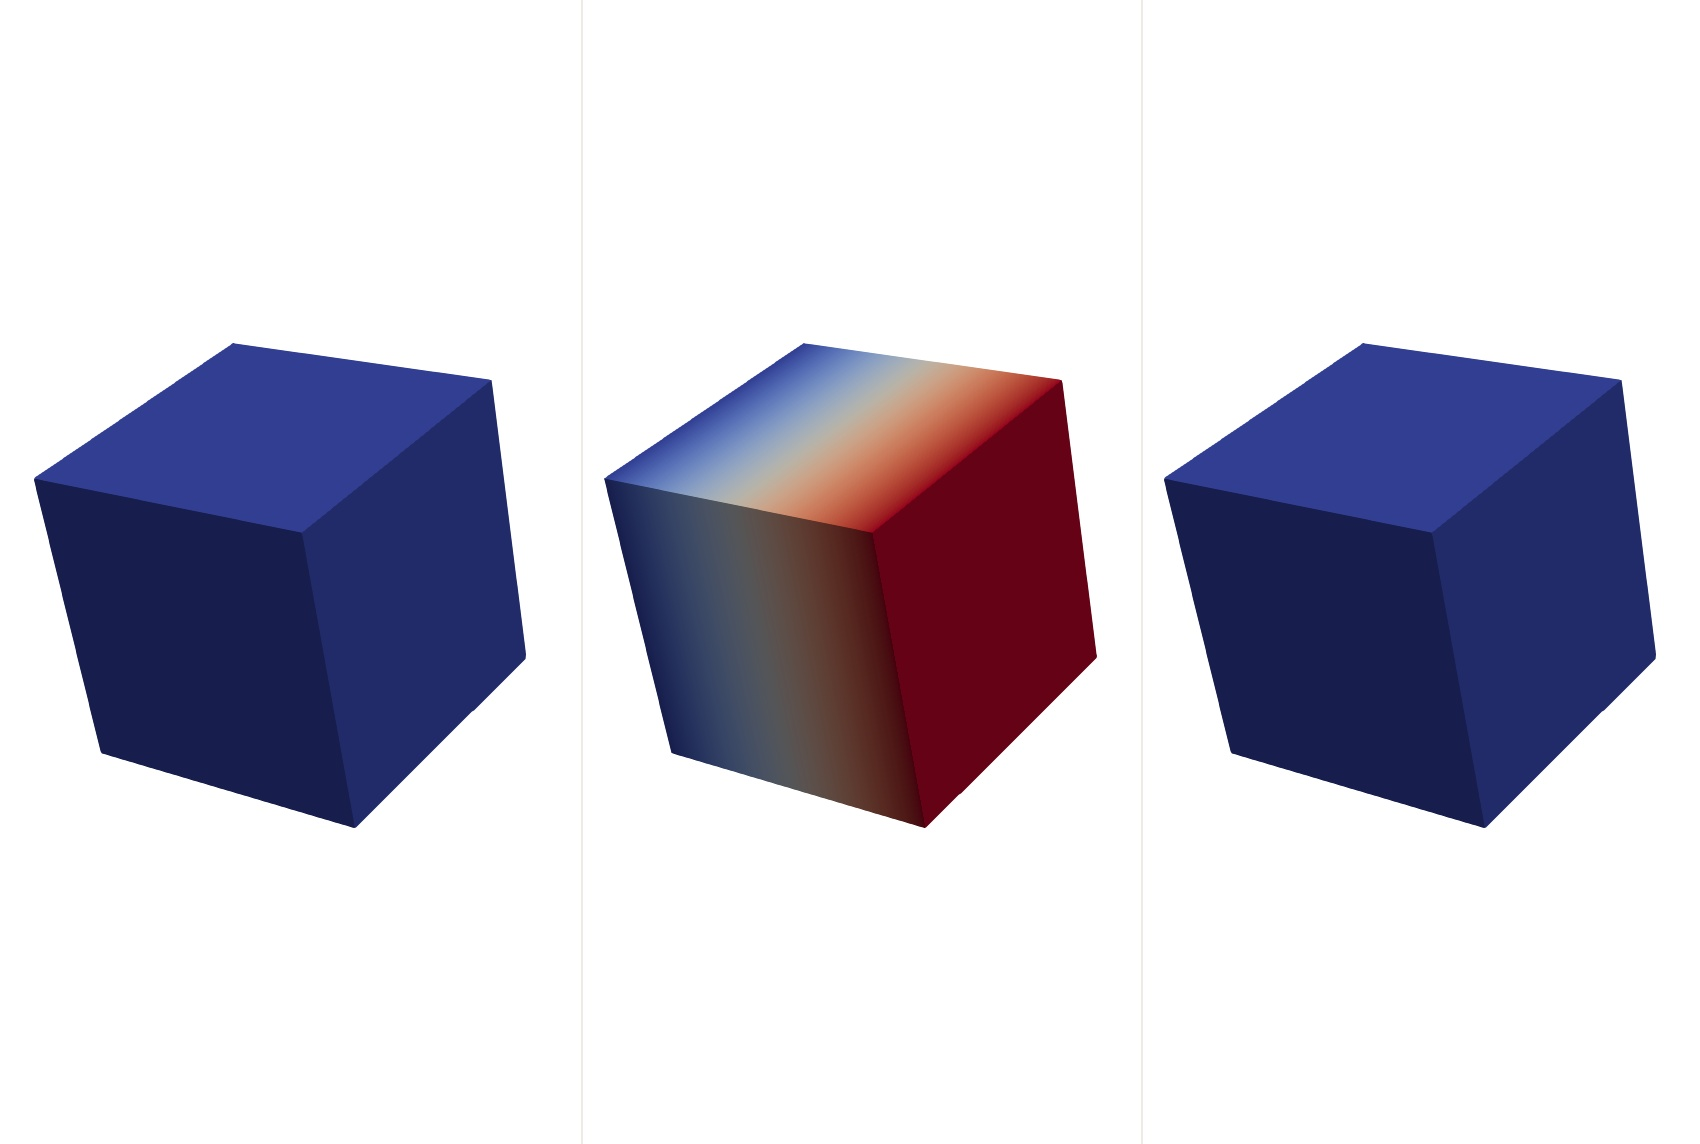
\includegraphics[width=0.3\textwidth]{img/basis/6.jpg}}\\
	\\	
	$\lo\begin{array}{c}0\\1\\0 \end{array}\ro$ & \raisebox{-0.5\totalheight}{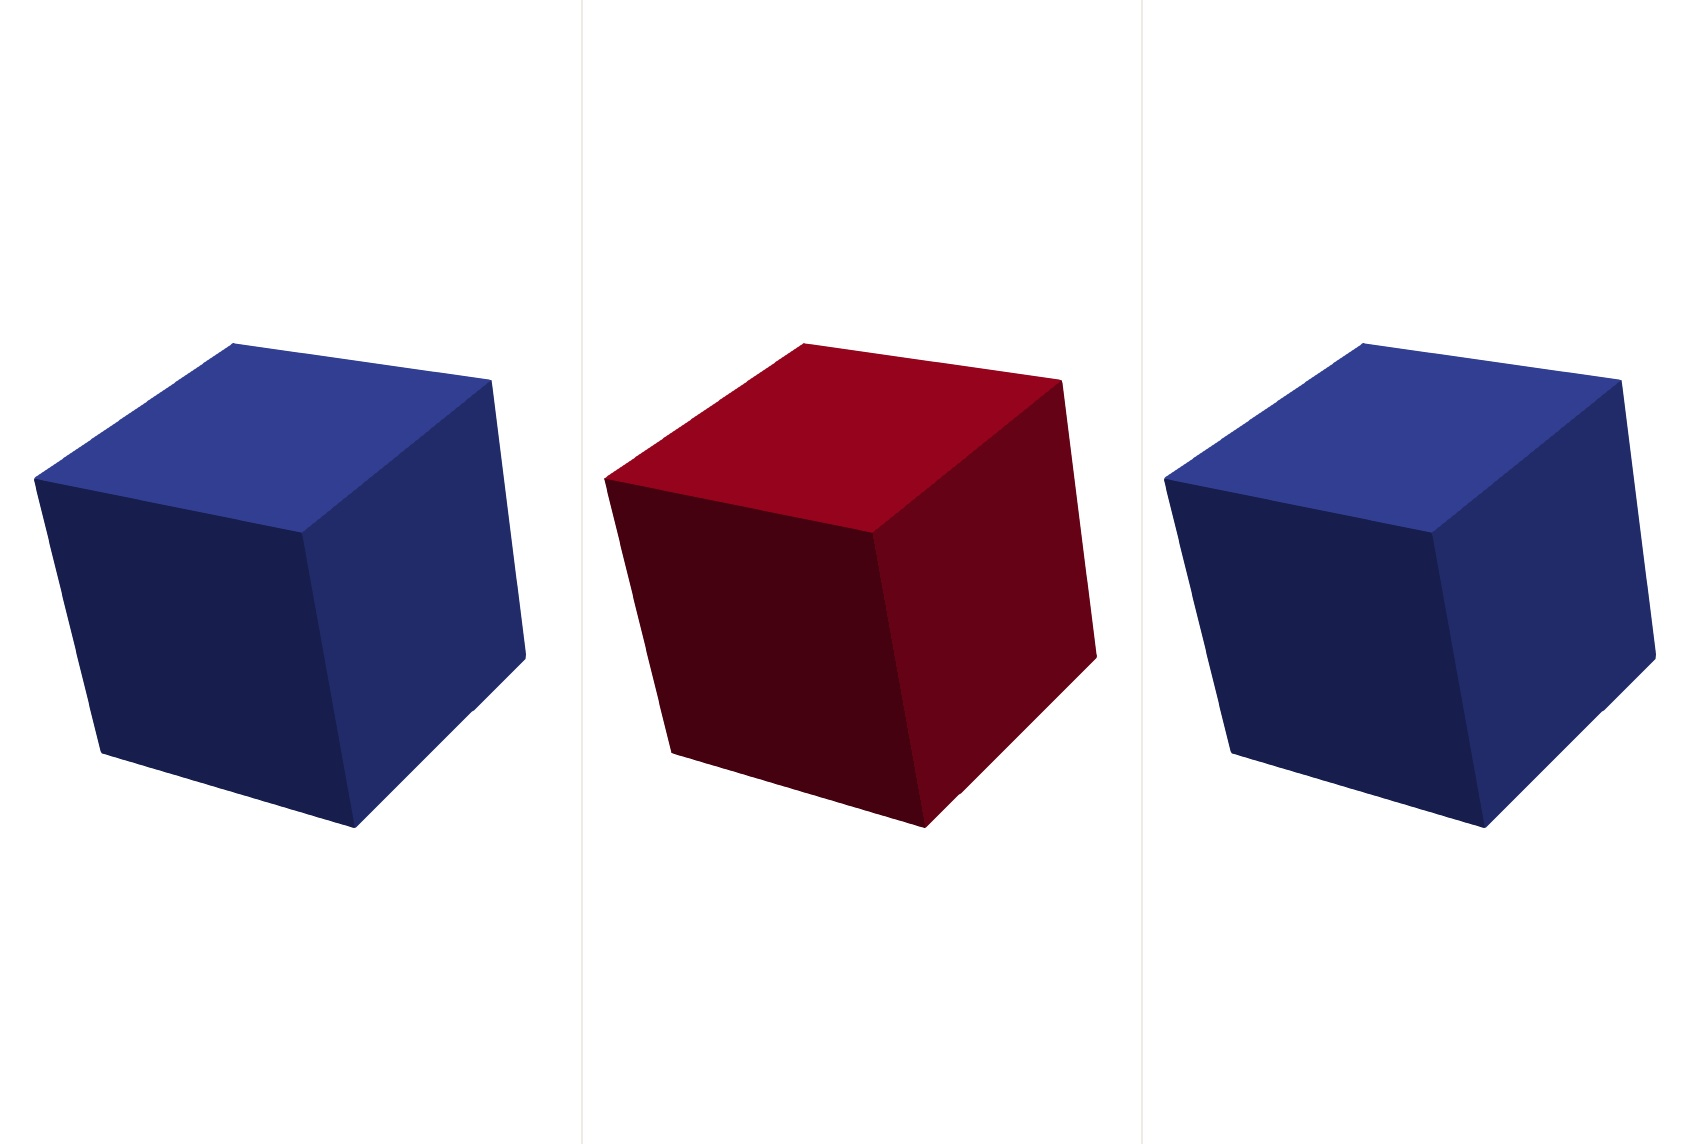
\includegraphics[width=0.3\textwidth]{img/basis/2.jpg}} & $\lo\begin{array}{c}z\\0\\0 \end{array}\ro$ & \raisebox{-0.5\totalheight}{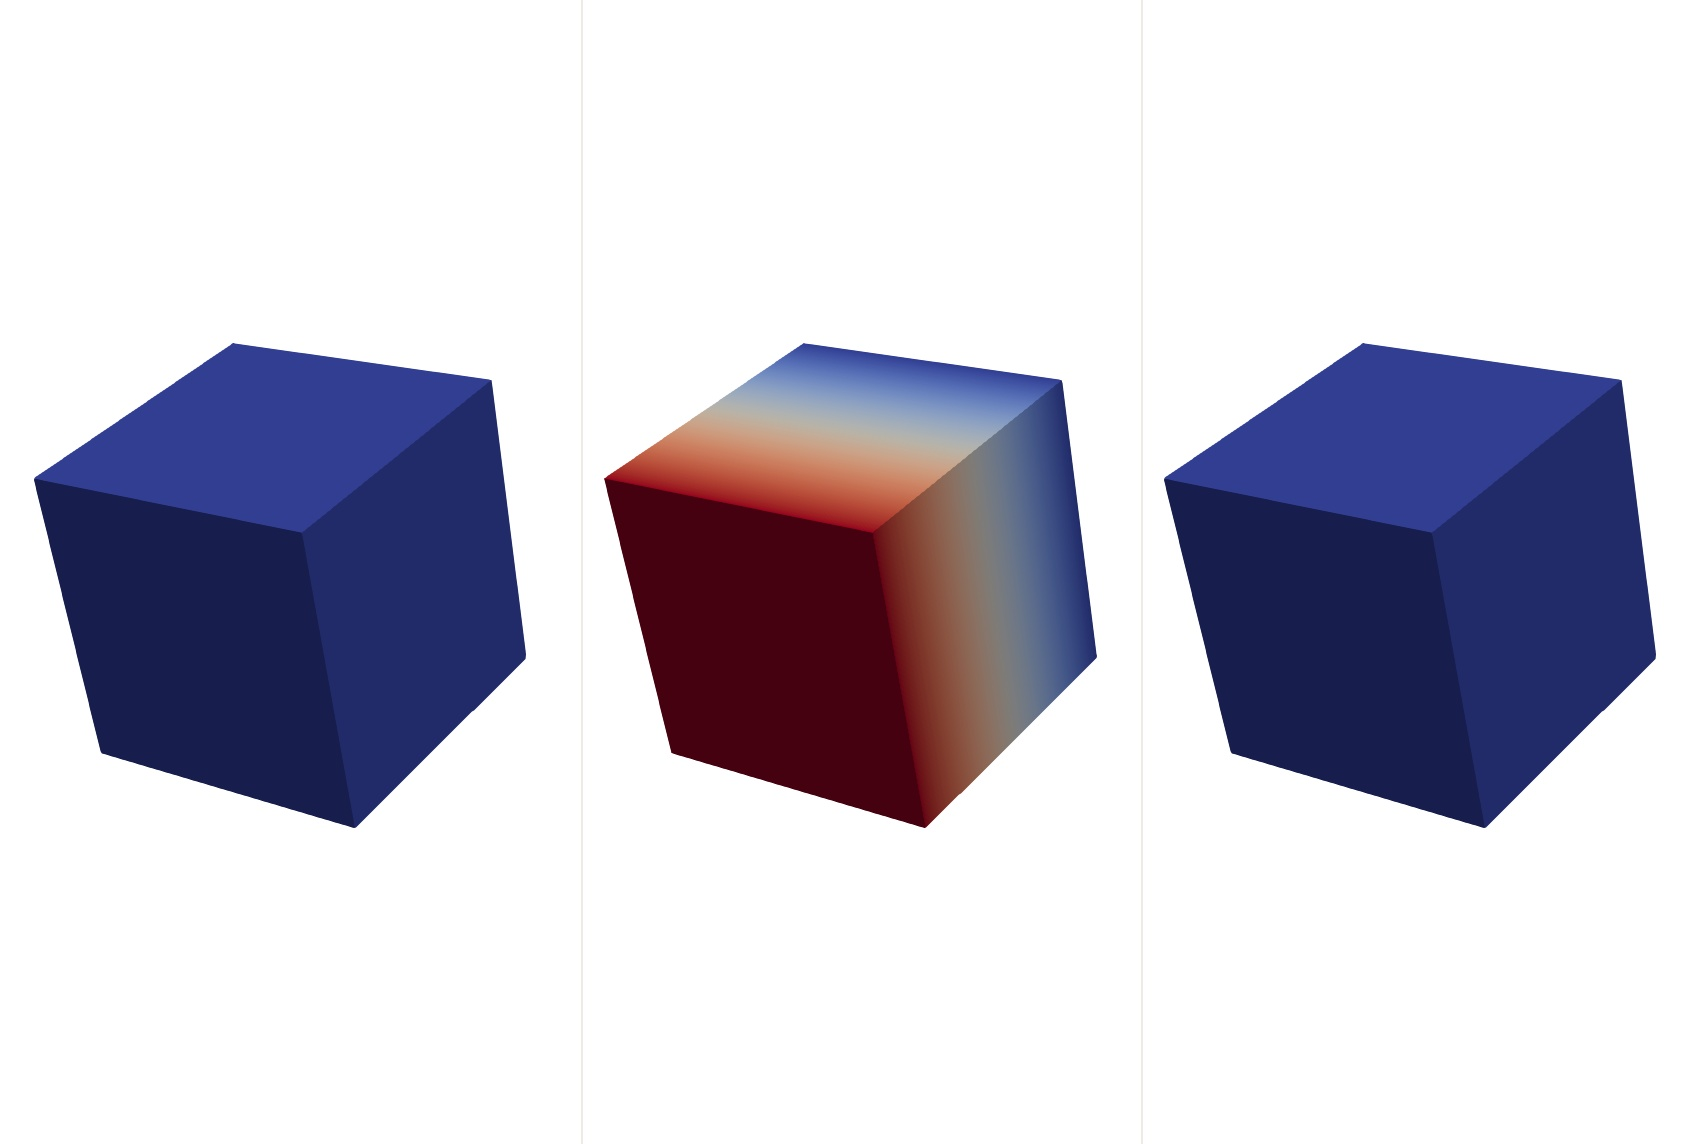
\includegraphics[width=0.3\textwidth]{img/basis/7.jpg}}\\
		\\	
	$\lo\begin{array}{c}0\\0\\1 \end{array}\ro$ & \raisebox{-0.5\totalheight}{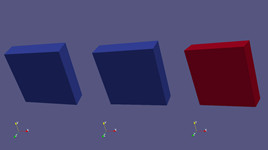
\includegraphics[width=0.3\textwidth]{img/basis/3.jpg}} & $\lo\begin{array}{c}0\\z\\0 \end{array}\ro$ & \raisebox{-0.5\totalheight}{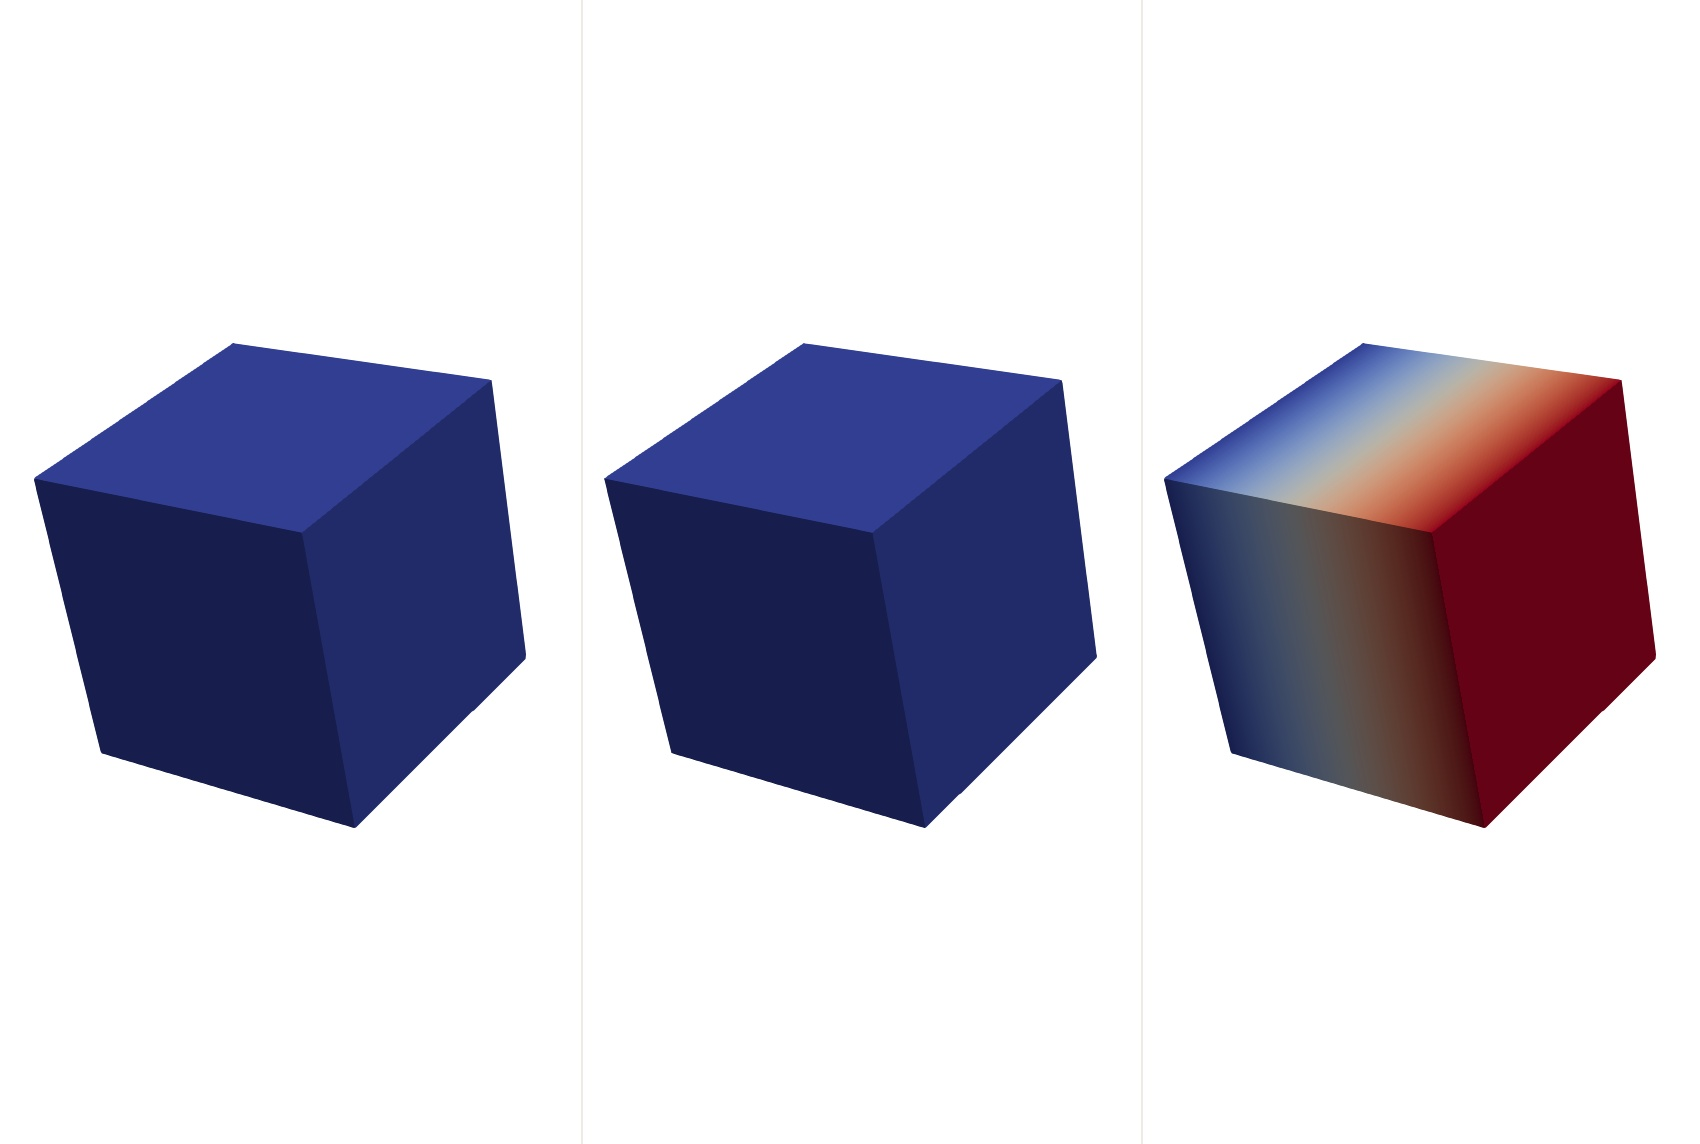
\includegraphics[width=0.3\textwidth]{img/basis/8.jpg}}\\
		\\	
	$\lo\begin{array}{c}y\\0\\0 \end{array}\ro$ & \raisebox{-0.5\totalheight}{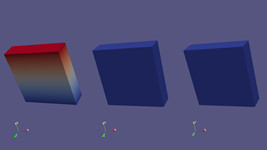
\includegraphics[width=0.3\textwidth]{img/basis/4.jpg}} & $\lo\begin{array}{c}0\\0\\x \end{array}\ro$ & \raisebox{-0.5\totalheight}{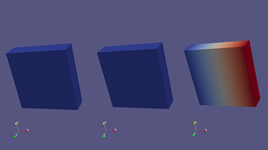
\includegraphics[width=0.3\textwidth]{img/basis/9.jpg}}\\
		\\	
	$\lo\begin{array}{c}0\\x\\0 \end{array}\ro$ & \raisebox{-0.5\totalheight}{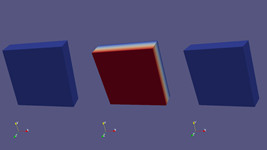
\includegraphics[width=0.3\textwidth]{img/basis/5.jpg}} & $\lo\begin{array}{c}2x\\-y\\-z \end{array}\ro$ & \raisebox{-0.5\totalheight}{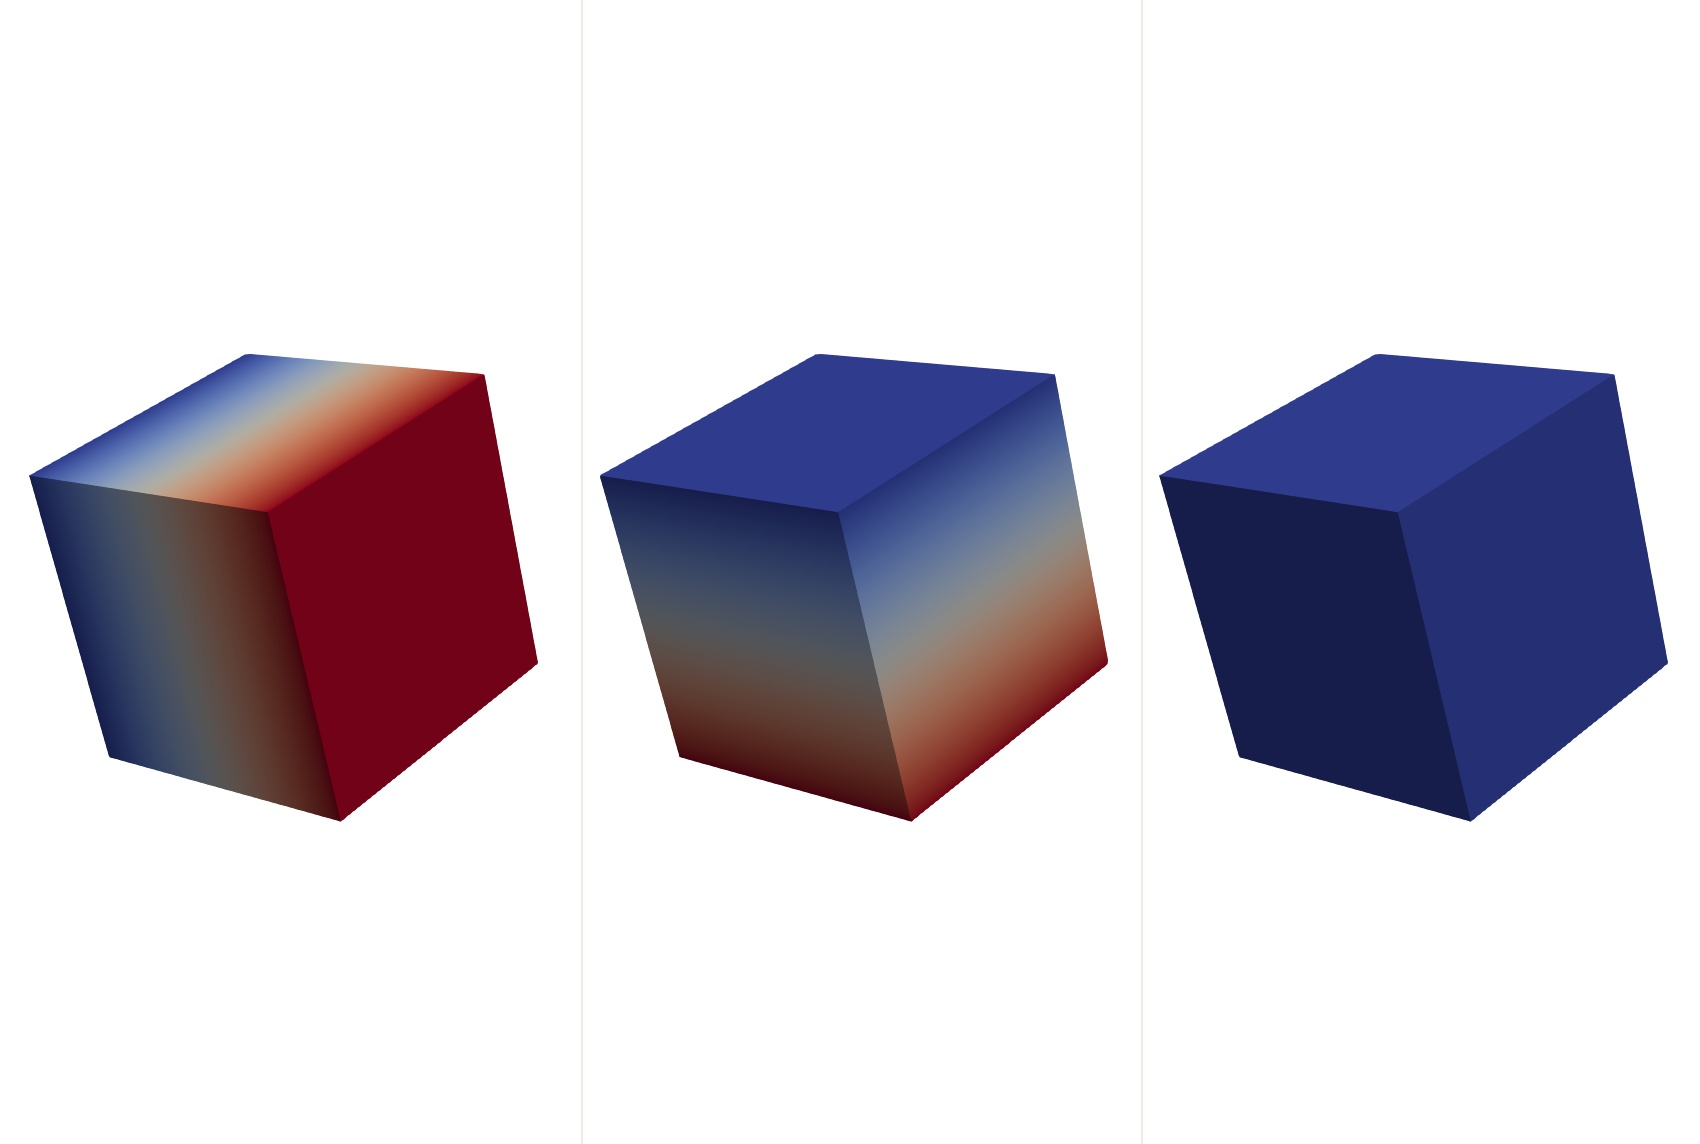
\includegraphics[width=0.3\textwidth]{img/basis/10.jpg}}\\	
	\\	
			\hline		
		\end{tabular*}
		\caption{Divergence-free space basis}
	\label{tbl:divFreeBasis}
\end{table}
In \ref{tbl:divFreeBasis}, it is obvious that only one function actually has more nonzero components.
\paragraph{}
In what follows, the notation $\left[V_h\right]^8$ used before will be used for the space where the last three components are replaced by $V_h^B$. Note that there are some technicalities with respect to the usage of $V_h^B$ needed to be handled in computation, e.g. in \ref{vertexBasedAlpha}, or later in \ref{Final_Integration_Fn}, \ref{Final_Integration_Fn_b} that we do not explicitly attend to.

\section{Discretization in time}
Relations \Cref{DG2} represent a system of ordinary differential equations which can be solved by a suitable numerical method. Since we are interested in applying the Rothe's method (as opposed to the method of lines, which switches the order of discretization in time and space), we now want to discretize the time derivative. In order to do so, we consider a partition $0 = t_0 < t_1 < t_2 < ...$ of the time interval $\lo 0, T\ro$ and set $\tau_k = t_{k+1} - t_k$. We use the notation $\bfw_h^k$ for the approximation of $\bfw_h\lo t_k\ro$.

\subsection{Discrete problem}
\label{section:discreteProblem}
Then we apply a time discretization scheme, for example, the simple explicit \emph{Euler method} and our \emph{fully discrete problem} reads: for each $k > 0$ find $\bfw_h^{k+1}$ such that
\begin{enumerate}
    \item ${\mrPsi_h}^{k+1} \in \left[V_h\right]^8$,
    \item For all test functions $\mrvh\in\left[V_h\right]^8$:
			\begin{align}
			\label{DiscretizedFull} \int_{\Omega_{t}} \frac{{\mrPsi_h}^{k+1} - {\mrPsi_h}^{k}}{\tau} \mrvh & - \sum_{K_i \in T_h}\int_{K_i}\mrF\lo{\mrPsi_h^{k}}\ro \lo\nabla \cdot \mrvh\ro\\
			\nonumber & + \sum_{\Gamma_{ij}\in\Gamma_I} \int_{\Gamma_{ij}} \mrH\lo{\mrPsi_h^{k}}|_{ij}, {\mrPsi_h^{k}}|_{ji}, \bfn_{ij}\ro \mrvh \\
			\nonumber & + \sum_{\Gamma_{ij}\in\Gamma_B} \int_{\Gamma_{ij}} \mrH\lo{\mrPsi_h^{k}}|_{ij}, \overline{{\mrPsi_h^{k}}|_{ji}}, \bfn_{ij}\ro \mrvh\\
			\nonumber & = \int_{\Omega_{t}} \mrS \mrvh,
			\end{align}
    \item ${\mrPsi_h}^{0}\lo\bfx\ro = \Pi_h \mrPsi^0\lo\bfx\ro$,
\end{enumerate}
where $\Pi_h$ is a projection of the initial condition $\mrPsi^0$ onto $\left[V_h\right]^8$.
\subsection{Time step length}
\label{section:CFL}
Time step length is an important attribute of the discretization. If it is too small, the calculation might be taking too long to finish, with unnecessary precision with respect to time. If it is too large, we may end up with unstable calculation and obtain results with nonphysical oscillations, or without a solution whatsoever. That is why we need to take extra care to derive the proper value. From the stability perspective, we have a condition for the upper bound of the time step - this condition is called the \textit{Courant-Friedrichs-Lewy} condition. This condition is of the following form:
\be
\label{CFLcond}
\tau_{max} = \text{min}\left\{\frac{{\Delta_{x}}_{min}}{c_{max}}, \frac{{\Delta_{x}}_{min}^2}{2 \eta_{max}}\right\},
\ee
where
${\Delta_{x}}_{min}$ is the smallest dimension of any element, $\eta_{max}$ highest resistivity in the domain, and $v_{max}$ highest velocity in the domain, where the following velocities are taken into account:
\begin{align}
c_s & =  \sqrt{\frac{\gamma\lo\gamma-1\ro}{\rho}\lo U - \rho v^2-U_B\ro},\\
c_a & =  \sqrt{\frac{B^2}{\rho}},\\
u,
\end{align}
where $c_s$ is the speed of sound, $c_a$ is the Alfv�n speed, and $u$ is the speed of plasma. We then take
$$
c_{max} = \text{max}\left\{c_s, c_a, u \right\}.
$$

\section{Algebraic formulation}
Last step in the DG method discretization is to transform the system of equations \Cref{DiscretizedLinear} into a system of linear algebraic equations at every time step $t_k$ and obtain the solution at this time step as the solution of this linear algebraic system.
\paragraph{}
First, we rearrange the system in the following manner:
\begin{align}
\label{RewrittenLinearSystem} \sum_{K_i \in T_h}\int_{K_i} \mrvh {\mrPsi_h}^{k+1} & = 
\sum_{K_i \in T_h}\int_{K_i} \left[{\mrPsi_h}^{k} + \tau\mrS + \tau\mrA\lo{\mrPsi_h^{k}}\ro \lo\nabla \cdot \mrvh\ro\right] \mrvh \\\nonumber& - \sum_{\Gamma_{ij}\in\Gamma_I} \int_{\Gamma_{ij}}\mrH\lo{\mrPsi_h^{k}}|_{ij}, {\mrPsi_h^{k}}|_{ji}, \bfn_{ij}\ro \mrvh
\\\nonumber& - \sum_{\Gamma_{ij}\in\Gamma_B} \int_{\Gamma_{ij}} \mrH\lo{\mrPsi_h^{k}}|_{ij}, \overline{{\mrPsi_h^{k}}|_{ji}}, \bfn_{ij}\ro \mrvh.
\end{align}
We can see that the left hand side does not depend on the previous solution values, so there is no need to recalculate the matrix entries in every time step (unless we employ AMR, in which case the mesh and therefore the set of basis functions changes).
Now
\be
\label{Coeffs} {\mrPsi_h}^{k+1} = \sum_{l = 0}^{l = L} y_l {\mrvh}_l, L = \mathrm{dim}\lo\left[V_h\right]^8\ro
\ee
for some (obviously finite) basis $\left\{{v_h}_1, ..., {v_h}_L\right\}$ of $\left[V_h\right]^8$.
Next, since $\mrPsi_h^{k}$, $\tau$, $S$, $\mrA$ (and the basis) are all known, we can define
\begin{align}
\label{Linear1}
a_{lm} & =  \sum_{K_i \in T_h}\int_{K_i} \mrvhl \mrvhm, \\
\label{Linear2}
b_{l} & =  \sum_{K_i \in T_h}\int_{K_i} \left[{\mrPsi_h}^{k} + \tau\mrS + \tau\mrA\lo{\mrPsi_h^{k}}\ro \lo\nabla \cdot \mrvhl\ro\right] \mrvhl\\\nonumber & - \sum_{\Gamma_{ij}\in\Gamma_I} \int_{\Gamma_{ij}}\mrH\lo{\mrPsi_h^{k}}|_{ij}, {\mrPsi_h^{k}}|_{ji}, \bfn_{ij}\ro \mrvhl\\\nonumber& - 
\sum_{\Gamma_{ij}\in\Gamma_B} \int_{\Gamma_{ij}} \mrH\lo{\mrPsi_h^{k}}|_{ij}, \overline{{\mrPsi_h^{k}}|_{ji}}, \bfn_{ij}\ro \mrvhl,\\
\label{Linear3}
A & =  \left\{a_{lm}\right\}_{l,m = 1}^{l,m = L},\\
\label{Linear4}
b & =  \left\{b_{l}\right\}_{l = 1}^{l = L},\\
y & =  \left\{y_{l}\right\}_{l = 1}^{l = L},
\label{Linear5}
\end{align}
and rewriting \Cref{RewrittenLinearSystem} using \Cref{Linear1} - \Cref{Linear5}, we come to the \textit{fully discrete algebraic problem at time instance $t_{k+1}$}:
\be
\label{Alg} Ay = b,
\ee
whose well-posedness, and other attributes that allow for a successful solution of this system, come from the properties of the DG method.
Now if we solve the system \Cref{Alg}, and obtain the solution vector $y$, we are able to reconstruct the discrete solution ${\mrPsi_h}^{k+1} \in \left[V_h\right]^8$ using the relation \Cref{Coeffs}.

In the implementation, we take the elements $K \in T_h$, of the triangulation $T_h$ to be rectangular hexahedra (rectangular parallelepipeds).
\section{Numerical integration}
Evaluation of the integral values in \ref{Linear1}, \ref{Linear2} is performed using the \textit{Gaussian numerical quadrature}. A quadrature rule approximates the integral values by replacing the integral as a weighted sum of integrand values at specified points in the domain of integration. The Gaussian quadrature is constructed so that the approximation is exact for polynomials of degree 2\textit{n} - 1 (and less). This is acceptable, as our space $V_h$ is constructed using polynomials - see section \ref{section:Vh} on the page \pageref{section:Vh}. We only need to take the value $n$ to be corresponding to the value of $p_m$ for the element $K_m$. The rule for both a 2-dimensional element face $\Gamma$, and a 3-dimensional cube $K$ is derived from a one-dimensional approximation (where the interval $\left[-1, 1\right]$ is a convention):
$$
\int_{-1}^1 f(x)\,dx = \sum_{i=1}^n w_i f(x_i),
$$
where the numbers $w_i > 0$ are the \textit{quadrature weights}, and the points (numbers in this case) $x_i$ are the \textit{quadrature points}, in the following way:
$$
\int_{\Gamma} f\lo\bfx\ro\,dx = \int_{-1}^{1}\int_{-1}^{1} f\lo x_1, x_2\ro\,dx \approx \sum_{i=1}^n\sum_{j=1}^n w_i w_j f\lo x_{1i}, x_{2j}\ro,
$$
$$
\int_{K} f\lo\bfx\ro\,dx = \int_{-1}^{1}\int_{-1}^{1}\int_{-1}^{1} f\lo x_1, x_2, x_3\ro\,dx \approx \sum_{i=1}^n\sum_{j=1}^n\sum_{k=1}^n w_i w_j w_k f\lo x_{1i}, x_{2j}, x_{3k}\ro,
$$
and transformation to a generic rectangular hexahedron (rectangular parallelepiped) is performed using the transformation in one dimension:
$$
\int_a^b f(x)\,dx \approx \frac{b-a}{2} \int_{-1}^1 f\left(\frac{b-a}{2}x + \frac{a+b}{2}\right)\,dx.
$$
Applying the Gaussian quadrature rule then results in the following one-dimensional approximation:
$$
\int_a^b f(x)\,dx \approx \frac{b-a}{2} \sum_{i=1}^n w_i f\left(\frac{b-a}{2}x_i + \frac{a+b}{2}\right).
$$
And the transformations in higher dimensions follow naturally. For $\Gamma = \left[a_1, b_1\right] \times \left[a_2, b_2\right]$ we have:
$$
\int_{\Gamma} f(x)\,d\bfx \approx \frac{b_2-a_2}{2}\frac{b_1-a_1}{2} \sum_{i=1}^n \sum_{j=1}^n w_i w_j f\lo\frac{b_1-a_1}{2}x_i + \frac{a_1+b_1}{2},\frac{b_2-a_2}{2}x_j + \frac{a_2+b_2}{2}\ro.
$$
Taking now e.g. \ref{Linear1}, and notation for quadrature points and weights, we can write (omitting the operand $\bfx = \lo x_1, x_2, x_3\ro$):
\begin{eqnarray}
a_{lm} & = & \sum_{K_i \in T_h}\int_{K_i} \mrvhl \mrvhm, \\
a_{lm} & := & \sum_{K_i \in T_h}\int_{K_i} f\lo\mrvhl, \mrvhm\ro , \\
a_{lm} & \approx & \sum_{K_i \in T_h} \sum_{\bfj=\overrightarrow{1}}^{\overrightarrow{n}} f\lo\mrvhl\lo\bfx_{\bfj}^i\ro, \mrvhm\lo\bfx_{\bfj}^i\ro\ro\,w_{\bfj},\label{Final_Integration_Fn}
\end{eqnarray}
where $\bfj$ is a multi-index used in sum over (volumetric) quadrature points $\bfx_{\bfj}^i \in K_i$.
Similarly for the right-hand side (\ref{Linear2}):
\begin{eqnarray}
b_{l} & = & \sum_{K_i \in T_h}\int_{K_i} \left[{\mrPsi_h}^{k} + \tau\mrS + \tau\mrA\lo{\mrPsi_h^{k}}\ro \lo\nabla \cdot \mrvhl\ro\right] \mrvhl\\\nonumber & - &\sum_{\Gamma_{ij}\in\Gamma_I} \int_{\Gamma_{ij}}\mrH\lo{\mrPsi_h^{k}}|_{ij}, {\mrPsi_h^{k}}|_{ji}, \bfn_{ij}\ro \mrvhl\\\nonumber& - &\sum_{\Gamma_{ij}\in\Gamma_B} \int_{\Gamma_{ij}} \mrH\lo{\mrPsi_h^{k}}|_{ij}, \overline{{\mrPsi_h^{k}}|_{ji}}, \bfn_{ij}\ro \mrvhl,\\
b_{l} & := & \sum_{K_i \in T_h}\int_{K_i} g\lo\mrvhl\ro - \sum_{\Gamma_{ij}\in\Gamma_I} \int_{\Gamma_{ij}}g^{'}\lo\mrvhl\ro - \sum_{\Gamma_{ij}\in\Gamma_B} \int_{\Gamma_{ij}} g^{''}\lo\mrvhl\ro \\
b_{l} & \approx & \sum_{K_i \in T_h} \sum_{\bfj=\overrightarrow{1}}^{\overrightarrow{n}} g\lo\mrvhl\lo\bfx_{\bfj}^i\ro\ro\,w_{\bfj}\\\nonumber & - & \sum_{\Gamma_{ij}\in\Gamma_I} \sum_{\bfj_f=\overrightarrow{1}}^{\overrightarrow{n_f}} g^{'}\lo\mrvhl\lo\bfx^{ij}_{\bfj_{f}}\ro\ro\,w_{\bfj_{f}}\\\nonumber & - & \sum_{\Gamma_{ij}\in\Gamma_B} \sum_{\bfj_{f}=\overrightarrow{1}}^{\overrightarrow{n_f}} g^{''}\lo\mrvhl\lo\bfx^{ij}_{\bfj_{f}}\ro\ro\,w_{\bfj_{f}},
\label{Final_Integration_Fn_b}
\end{eqnarray}
where in addition to $\bfj$ as explained before, $\bfj_{f}$ is a multi-index used sum over face quadrature points $\bfx_{\bfj_f}^{ij} \in \Gamma_{ij}$. Based on this, we can define
\begin{eqnarray}
\label{singleNumIntA}
a_{lmi \bfj} & = & f\lo\mrvhl\lo\bfx^i_{\bfj}\ro, \mrvhm\lo\bfx^i_{\bfj}\ro\ro\,w_{\bfj},\\
\label{singleNumIntB}
b_{li \bfj} & = & g\lo\mrvhl\lo\bfx^i_{\bfj}\ro\ro\,w_{\bfj},\\
\label{singleNumIntBface}
b^{'}_{lij \bfj_f} & = & \left\{\begin{array}{c} g^{'}\lo\mrvhl\lo\bfx^{ij}_{\bfj_f}\ro\ro\,w_{\bfj}\ \ if\ \Gamma_{ij}\in \Gamma_I \\ g^{''}\lo\mrvhl\lo\bfx^{ij}_{\bfj_f}\ro\ro\,w_{\bfj}\ \ if\ \Gamma_{ij}\in \Gamma_B \end{array}\right. .
\end{eqnarray}

\section{Assembling the algebraic problem}
Now we have a clear expression how to evaluate the integral values \ref{Linear1}, \ref{Linear2} using \ref{singleNumIntA}, \ref{singleNumIntB}, \ref{singleNumIntBface}, but we need to construct the matrix $A$ (\ref{Linear3}), and the right-hand-side vector $b$ (\ref{Linear4}) in an effective manner.
This is generally achieved through a \textit{element-wise} assembling of these structures. Key to this is to create a data structure that identifies for a particular element $K_i$ all the test functions $\mrvhl$ that make sense to be evaluated (have non-empty support) on $K_i$, i.e. we are looking for the set
\be
\mrvh \lo K_i \ro = \left\{\mrvh \in V_h : supp\lo\mrvh\ro \cap K_i \neq \emptyset \right\},
\ee
and do the same for the faces $\Gamma_i$ (both boundary, and internal):
\be
\mrvh \lo \Gamma_i \ro = \left\{\mrvh \in V_h : supp\lo\mrvh\ro \cap \Gamma_i \neq \emptyset \right\}.
\ee
Now the assembling procedure looks like this:\\
\begin{algorithm}[H]
    \# 1 - Loop over elements\\
    \ForEach{$K_i\in T_h$}{
       \KwData{Quadrature points $\left\{\bfx^i_1, ..., \bfx^i_{\bfn}\right\}$}
       \KwData{Jacobian of the mapping $J_{K_i}$ mapping the reference element (unit cube) to the actual element}
       \KwData{Quadrature weights $\left\{w_1, ..., w_{\bfn}\right\}$}
                   \# Loop over quadrature points\\
       \ForEach{$\bfj \in \left\{1, ..., \bfn\right\}$}{
           \textbf{Set: }$\lo JxW\ro_{\bfj} = J_{K_i} \times w_{\bfj}$\\
            \# Loop over test functions\\
        \ForEach{$v\in v_h \lo {K_i} \ro$}{
       \KwData{$l$ - index of $v$ in the global system, i.e. row in \ref{Linear3} - \ref{Linear5}}
                        \# Loop over basis functions\\
            \ForEach{$u\in v_h \lo {K_i} \ro$}{
       \KwData{$m$ - index of $u$ in the global system, i.e. column in \ref{Linear3}}
                
                        $a_{lm}\ \ +=\ \ \lo JxW\ro_{\bfj} \ a_{lmi \bfj}$
                    }

                $b_{l}\ \ +=\ \ \lo JxW\ro_{\bfj} \ b_{li \bfj}$
        }                
        }
    }
\ \\
        \# 2 - Loop over edges\\
        \ForEach{$\Gamma_{ij}\in T_h$}{
            \KwData{Quadrature points $\left\{\bfx^{ij}_1, ..., \bfx^{ij}_{\bfn_f}\right\}$}
            \KwData{Jacobian of the mapping $J_{K^+} = J_{K^-}$ mapping the reference face (unit square) to the actual face, where $K^+, K^-$ are elements adjacent to $\Gamma_{ij}$ if this is an internal edge, or $K^+ = K^-$ if this is a boundary edge.}
            \KwData{Quadrature weights $\left\{w_1, ..., w_{\bfn_f}\right\}$}
            \# Loop over quadrature points\\
            \ForEach{$\bfj_f \in \left\{1, ..., \bfn_f\right\}$}{
                \textbf{Set: }$\lo JxW\ro_{\bfj_f} = {J_K}^{+} \times w_{\bfj_f}\ $ \# Here it does not matter if we choose $J_{K^+}$ or $J_{K^-}$\\
                \# Loop over test functions\\
                \ForEach{$v\in v_h \lo K^+ \ro$}{
                    \KwData{$l$ - index of $v$ in the global system, i.e. row in \ref{Linear3} - \ref{Linear5}}
                    
                    $b_{l}\ \ +=\ \ \lo JxW\ro_{\bfj_f} \ b^{'}_{lij \bfj_f}$
                }
            }
        }
\caption{Assembling of the algebraic problem \ref{Alg}}
\label{algorithm:singleTimeStep}
\end{algorithm}
An important remark needs to be added here, with respect to the fact, that we aim for a distributed computation. As stated before, the domain decomposition approach leads to each of the processors $P_i \in \left\{P_0, ..., P_N\right\}$ of the total number of processors employed for the computation owning only a subset of elements $\left\{K \in T\right\}_i$. If the processor $P_i$ did not have any data about other elements, we would not be able to perform the evaluation involving $b^{'}$ defined in \ref{singleNumIntBface}, or more precisely $g^{'}$ defined in \ref{Final_Integration_Fn_b} as the values ${\mrPsi_h^{k}}|_{ji}$ for edges $\Gamma_{ij}$ of elements from $\left\{K \in T\right\}_i$ will not always be there.
\paragraph{}
To amend this situation, in the distributed triangulation, each processor holds not only the mesh element data it owns, but also data for mesh elements it needs - in Discontinuous Galerkin method, for exactly the purposes of internal face integral evaluation described in the previous paragraph. This data is called \textit{ghost elements}, or \textit{ghost cells}, as these are only copies provided by other processors which own the particular elements.

TODO obrazek domain decomposition s ghost cell layer

\paragraph{}
Note that in the described algorithm, and also with respect to the remarks in the previous paragraphs, periodic boundary conditions are not specifically handled, as they are only a technically more complex case of internal edges (both from the perspective of necessity of utilizing ghost cells, and from the perspective of evaluating $b_{l}$ in \ref{algorithm:singleTimeStep}.

%\section{Calculation considerations}
%
%\subsection{Stability}
%
%\subsection{Convergence}
%
%\subsection{Dissipation}

\section{Time-stepping and linearization}

\subsection{Time-stepping}
The simple time discretization scheme that we use in \cref{section:discreteProblem} allows us to simply implement the time-stepping in the following fashion:\\
\begin{algorithm}[H]
\textbf{    Set: }$y_0 =\ $ (initial solution)\\
\textbf{    Set: }$ts = 1 $ \# initial time step\\
\textbf{    Set: }$t = 0.00 $ \# initial time\\
    \# Loop over time steps\\
    \For{$;\ t < T;\ t = t+\tau,\ ts = ts + 1$}{
        \KwData{Solution from the previous time step $y^{ts - 1}$}
1.Call procedure \cref{algorithm:singleTimeStep} to obtain $A, b\lo y^{ts - 1}\ro$\\
2.Solve the problem $Ay^{ts} = b\lo y^{ts - 1}\ro\ $ \# See note below\\
3.(If necessary) postprocess $y^{ts}$ using \cref{algorithm:limiter}\\
4.Calculate updated value of $\tau$ using \cref{equation:CFLcond}\\
	 }
    \caption{Time-stepping procedure}
\label{algorithm:timeStepping}
\end{algorithm}
\paragraph{Note}
\label{note:solvers}
The step 2 (solving the algebraic problem) is of course a key point in the overall process. Because of its importance, the aim of this work is not to describe, or even implement an algebraic solver for this purpose. Many scientific teams have spent many years on publicly available open-source solvers that are usable by the software we develop for the purpose of solving the MHD phenomena. We use the existing solvers.

\section{Performance considerations}
Since eventually results are obtained by running a (distributed) program that implements the numerical methods, it is important to focus also on the performance aspects of the implementation, and not only on the numerical schemes. Plainly put, even a very efficient numerical algorithm can run on a computer a very long time, if not implemented properly.
\subsection{Parallelization}
\label{section:parallel}
To be able to perform any large scale calculations, we need to be able to utilize the performance of hardware at maximum. Being able to use modern, multi-core computers is an absolute must to achieve good performance, as the execution time when using parallel execution can decrease by a factor of corresponding to the number of cores - and modern machines have tens of cores available.

The parallelization is possible at several places in the overall algorithm \cref{algorithm:singleTimeStep}. But it makes most sense to parallelize the outer-most loop over elements, and over faces.

\paragraph{}
Another point for parallelization is the algebraic solver. As explained in \cref{note:solvers}, we rely on existing software packages for finding the solution of the algebraic system \cref{Alg} - all the used solvers support and heavily utilize parallelization.

\subsection{Vectorization}
Similarly as in section \cref{section:parallel}, the goal here is to be able to solve the discretized problem in the most efficient (fastest) way possible. One of the features that (modern) hardware offers is to employ vectorization instructions - i.e. unary or binary instructions that operate on $N, N > 1$ values (in case of unary instructions), or $N, N > 1$ pairs of values (in case of binary instructions) at the same time - the number $N$ depends on the capabilities of the CPU, and on the precision (single or double). On the hardware that was available to perform calculations for this thesis (and based on always-used double precision), $N = \left\{4, 8\right\}$, using such instructions requires both using them in the code (one has to specify that these instructions shall be generated explicitly), and having the compiler aware of these, and able to utilize them in the generated machine code - both compilers used for work on this thesis (GNU gcc, and Microsoft Visual Studio) support vectorization instructions (SSE, SSE2, AVX, AVX2).
\paragraph{}
Vectorization helps heavily with respect to CPU time spent on calculation. In the algorithm \cref{algorithm:singleTimeStep}, vectorized instructions are used in:
\begin{itemize}
    \item evaluation of the expressions $a_{lm} += JxW_{\bfj} \ a_{lm K \bfj}$
    \item evaluation of expressions $b_{l} += JxW_{\bfj} \ b_{l K \bfj}|_{face|volumetric}$
    \item calculation of $JxW_{\bfj}$
\end{itemize}

\subsection{Distribution}
As discussed in \cref{section:ditributedTria}, the \textit{domain decomposition} approach is taken to overcome the physical limitations (CPU physical size, RAM capacity, ...) of a single machine with shared memory.
\paragraph{}
This approach has several aspects, that are worth mentioning. The entire process of discretization of MHD equations (as well as any other system of PDEs) eventually leads to solving large (sparse) systems of linear equations, and then interpretation of the solution in terms of a global (defined on entire $\Omega$) function - that is a linear combination of the global basis functions with the solution of the linear problem being the coefficients of this linear combination. From this it follows, that distributing only the triangulation would not by itself lead to radical increase of the size of problems we can tackle, there are other points where the algorithms employed need to take distribution of data among processors into account:
\begin{enumerate}
	\item
		Distributed matrix and right hand side
		\begin{itemize}
			\item It is necessary for each processor to be able to utilize the memory on the node it physically belongs to when writing values of calculated integrals into the algebraic structure (see steps $a_{lm}\ +=...$, $b_{l}\ +=...$ of \cref{algorithm:singleTimeStep}).
			\item Distribution of the matrix is actually very important from the memory capacity perspective. It is typically the largest data structure (together with preconditioner) used in the entire implementation - regardless whether the used method is FEM, DGFEM, or Finite Volumes for example.
		\end{itemize}
	\item
		Distributed algebraic solver
	When the algebraic structures (the matrix and the right hand side) are completed, the sought solution must again be sought in a distributed manner, otherwise the added cost would be transferring algebraic data from all processors to a common one, where the solution would be sought. This is, however, a theoretical possibility, as the data structures used in the solution of the algebraic problem (decompositions, preconditioners, ...) are typically too large to be stored on a single processor anyway.
	\item
		Distributed solution
		\begin{itemize}
			\item Although it is quite obvious, it is noteworthy that as the algebraic structures are distributed, and so is the solution of the algebraic problem, the actual solution is again, distributed according to the domain decomposition.
			\item The distributed solution is the data structure that is most important from the perspective of the \textit{ghost cells} - illustrated in \cref{figure:ghost}, where for the distributed discontinuous Galerkin method, we need to be able to access the distributed solution values from all neighboring elements when performing numerical integration \cref{singleNumIntBface}.
		\end{itemize}
\end{enumerate}
\subsubsection{Message Passing Interface and deal.II}
For all distributed computing purposes in this work, deal.II implementation of the Message Passing Interface (MPI) was used. MPI is a specification for a standard library for message passing for the purposes of distributed computing, and was originally introduced in \cite{mpi}. The library deal.II (\cite{deal}) offers wrappers for low-level MPI functions, that are utilizable in the implementation of the methods of this work.


\chapter{Adaptive Mesh Refinement}
\label{chapter:amr}
As the Adaptive Mesh Refinement (AMR) is a very important algorithm in the overall numerical solution, handling the multi-scale aspect of the studied problems, in this chapter, a description of what needs to be taken care of for the DG method, in the distributed settings, and what concrete decisions were made during this work, and justification of these in light of the requirements on the numerical solution.
\paragraph{}
Note that in what follows, the symbol $T$ or $T_{i\in\left\{0, 1, 2, ...\right\}}$ shall denote a general computational mesh and a particular mesh in the series of refined meshes respectively. We shall drop the subscript $h$ from $T_h$ referring to the dimension (maximum of diameters of all elements) of the mesh where possible.

\section{Overview of the AMR}
The general schema of any Adaptive Mesh Refinement algorithm is described in the algorithm \Cref{algorithm:AMRGen}:
\ \\
\begin{algorithm}[H]
 \KwData{Mesh $T_0$}
 \KwResult{A mesh $T_n$ and a solution $\bfy_n$ on this mesh satisfying the solution acceptance criteria}
 i = 0\\
 \While{true}{
  obtain solution $\bfy_i$ on $T_i$\\
	evaluate solution $\bfy_i$ acceptance criteria\\
	\eIf{solution acceptance criteria satisfied} {
		return\\
   } {
		identify subset $T^{r}_i$ of all elements $K \in T_i$ to be refined, $T^{r}_i \subseteq T_i$\\
		obtain $T_{i+1}$ by refining (at least) all $K \in T^{r}_i$\\
		i = i + 1\\
	}
 }
 \caption{Generic AMR algorithm}
\label{algorithm:AMRGen}
\end{algorithm}
In \Cref{algorithm:AMRGen}, \textit{solution acceptance criteria} is usually either spatial error estimate threshold, or number of elements, etc. In the same description, the note that there might be other elements $K \notin T^{r}_i$ refined in order to maintain some desired attributes of the mesh, such as 1-irregularity (the refinement level difference of two elements sharing a common face is at most one), smoothness of mesh (there is e.g. no unrefined elements for which all, or a majority of neighboring elements would be refined), etc.
An example of several steps of the algorithm (where step number corresponds to the variable $i$ in \Cref{algorithm:AMRGen}, is given in \Cref{figure:amrsimple} below on a sample problem in 2 dimensions.

\begin{figure}[H]
	\begin{subfigure}[H]{40mm}
					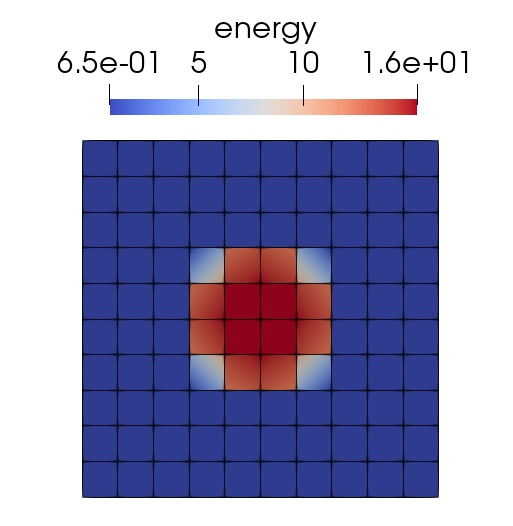
\includegraphics[width=\textwidth]{img/adapt/sln0.jpg}
					\caption{AMR step 0 - 100 elements}
	\end{subfigure}
	\hspace{7mm}
	\begin{subfigure}[H]{40mm}
					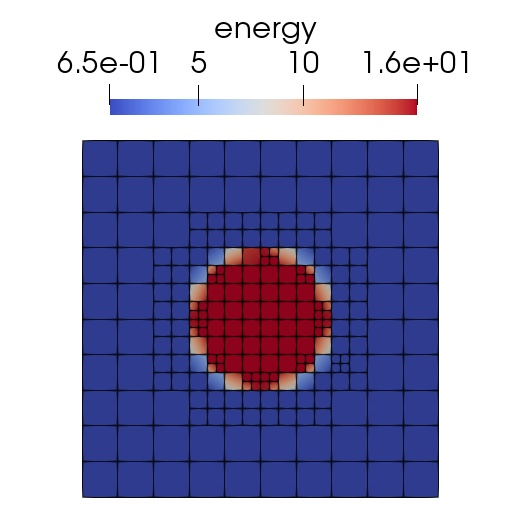
\includegraphics[width=\textwidth]{img/adapt/sln1.jpg}
					\caption{AMR step 1 - 232 elements}
	\end{subfigure}
	\hspace{7mm}
	\begin{subfigure}[H]{40mm}
					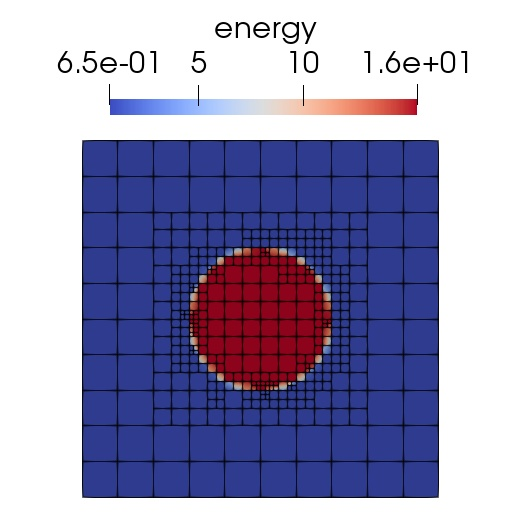
\includegraphics[width=\textwidth]{img/adapt/sln2.jpg}
					\caption{AMR step 2 - 379 elements}
	\end{subfigure}
	\\
	\begin{subfigure}[H]{40mm}
					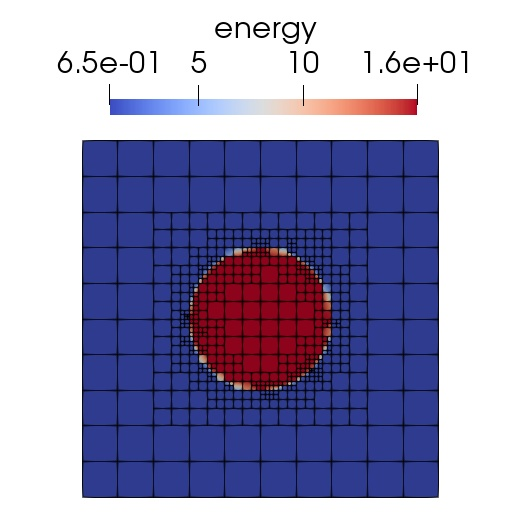
\includegraphics[width=\textwidth]{img/adapt/sln3.jpg}
					\caption{AMR step 3 - 610 elements}
	\end{subfigure}
	\hspace{7mm}
	\begin{subfigure}[H]{40mm}
					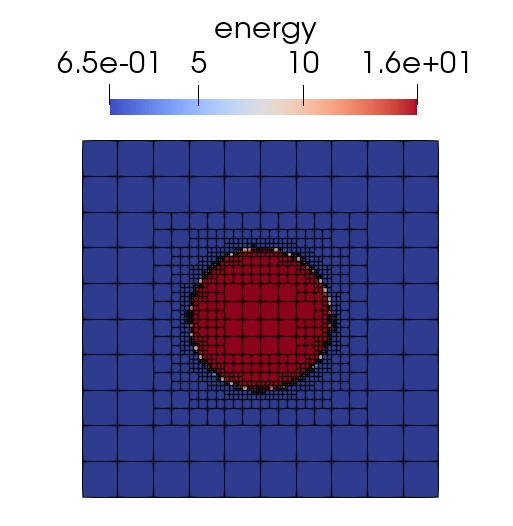
\includegraphics[width=\textwidth]{img/adapt/sln4.jpg}
					\caption{AMR step 4 - 1016 elements}
	\end{subfigure}
	\hspace{7mm}
	\begin{subfigure}[H]{40mm}
					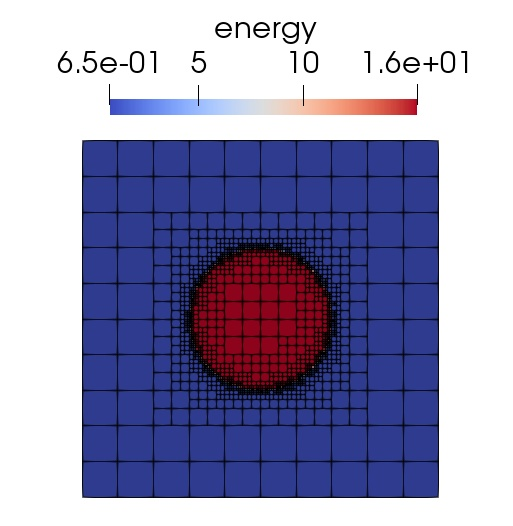
\includegraphics[width=\textwidth]{img/adapt/sln5.jpg}
					\caption{AMR step 5 - 1364 elements}
	\end{subfigure}
		\vspace{3mm}
	\caption{AMR steps}
	\label{figure:amrsimple}
\end{figure}

The benefit of AMR is clear. If we were to discretize the entire domain with elements small enough to capture the solution with the same quality as in the last AMR step, we would end up with $> 40000$ elements, where with AMR, the same is achieved with $< 1400$.

\paragraph{}
Since we are dealing with evolution equations, it is necessary to specify how the AMR algorithm relates with the non-AMR solution algorithm \Cref{algorithm:timeStepping}. There are several points we need to take into considerations:
\begin{itemize}
	\item slope limiting as a postprocessing step after the solution must not be omitted in case of higher-order (e.g. linear) basis functions
	\item the solution needs to be transferred to the refined mesh in order to be able to assemble the matrix and the right-hand side on the refined mesh in the next adaptivity iteration
	\item since the solution evolves and the refinements that contribute to error reduction at time step $n$ do not contribute to error reduction at time step $n + m$ (the solution was e.g. oscillating or potentially discontinuous at time step $n$, but is smooth at time step $n + m$), we also want to revert such refinements as the simulation time progresses, we call this process \textit{coarsening} of elements. For this we shall define a set $T^{c}_i$ of all elements to be coarsened.
\end{itemize}
The algorithm looks like this:

\begin{algorithm}[H]
\textbf{    Set: }$y_0 =\ $ (initial solution)\\
\textbf{    Set: }$ts = 1 $ \# initial time step\\
\textbf{    Set: }$t = 0.00 $ \# initial time\\
    \# Loop over time steps\\
    \For{$;\ t < T;\ t = t+\tau,\ ts = ts + 1$}{
			\KwData{Solution from the previous time step $y^{ts - 1}$ expressed on the mesh $T^{ts}_0$}
			 i = 0\\
			 \While{true}{
				call procedure \Cref{algorithm:singleTimeStep} to obtain $A_{i}, b_{i}\lo y^{ts - 1}_{i}\ro$ on the mesh $T^{ts}_i$\\
				solve the problem $A_i y^{ts}_i = b_{i}\lo y^{ts - 1}_i\ro$\\
				post-process the solution $y^{ts}_i$ using \Cref{algorithm:limiter}\\
				evaluate solution $y^{ts}_i$ acceptance criteria\\
				\eIf{solution acceptance criteria satisfied} {
					$y^{ts} = y^{ts}_i$\\
					break While loop\\
				 } {
					identify subset $T^{r}_i$ of all elements $K \in T^{ts}_i$ to be refined, $T^{r}_i \subseteq T^{ts}_i$\\
					identify subset $T^{c}_i$ of all elements $K \in T^{ts}_i$ to be coarsened, $T^{c}_i \subseteq T^{ts}_i$\\
					obtain $T^{ts}_{i+1}$ by refining (at least) all $K \in T^{r}_i$ and coarsening a subset of $T^{c}_i$\\
					transfer the solution $y^{ts}_i$ onto $T^{ts}_{i+1}$\\
					i = i + 1\\
				}
		 }
			calculate updated value of $\tau$ using \Cref{equation:CFLcond}\\
	 }
\caption{AMR for time-discretized problems}
\label{algorithm:AMRFull}
\end{algorithm}

TODO - tady time dep.

The critical points of the algorithm \Cref{algorithm:AMRFull}are
\begin{itemize}
\item solution acceptance criteria evaluation,
\item identification of subset $T^{r}_i$,
\item identification of subset $T^{c}_i$.
\end{itemize}
For the last two points, we shall consider a function $r$
\be
\label{refinementIndicator}
r:\ T^{ts}_i \rightarrow [0, +\infty),
\ee
which shall be called \textit{refinement indicator}, and the set $T^{r}_i = \left\{K^{r}\right\}$ shall be then defined as a set of all such elements for which one of these criteria are satisfied:
\be
	\label{refIndicatorValues}
	r\lo K^{r}\ro > \alpha \cdot \max\left\{r\lo K\ro\ |\ K \in T^{ts}_i\right\} \text{, or}
\ee
\be
	r\lo K^{r}\ro > \beta \cdot \sum\left\{r\lo K\ro\ |\ K \in T^{ts}_i\right\}.
\ee

The set $T^{c}_i = \left\{K^{c}\right\}$ shall be defined similarly as
\be
	r\lo K^{c}\ro < \gamma \cdot \max\left\{r\lo K\ro\ |\ K \in T^{ts}_i\right\} \text{, or}
\ee
\be
	\label{refIndicatorValuesEnd}
	r\lo K^{c}\ro < \delta \cdot \sum\left\{r\lo K\ro\ |\ K \in T^{ts}_i\right\}.
\ee

Note that the parameters $0 < \gamma \leq \alpha < 1,\ 0 < \delta \leq \beta < 1$ are artificial, and do not affect the overall solution quality (as the solution acceptance criteria has to be met independently of choices of their values). Nevertheless, the choices may affect performance - e.g. for a high $\alpha, \beta$, many steps are needed in order to satisfy the solution acceptance criteria, and on the other hand, if values are too low, there is an unnecessary high number of degrees of freedom that do not contribute substantially to the reduction of the solution error.
\paragraph{}
Please also note, that description of edge cases, and limitations are not given here for brevity. These cases include e.g. what happens if an element is both selected for coarsening and refinement, or how we maintain a 'minimal' refinement level so that we do not coarsen beyond a rational limit.

\section{Adaptive-mesh refinement and DG}
With the Discontinuous Galerkin method, using AMR brings additional complexity into the evaluation of face integrals described in \Cref{Final_Integration_Fn_b}, \Cref{singleNumIntBface}.
To describe the process in detail, definition of the numerical flux \Cref{NumFluxDef} needs to be taken into account. What is evaluated during the assembling procedure \Cref{algorithm:singleTimeStep} is the term \Cref{singleNumIntBface}. In order to evaluate 

TODO obrazky moznych pripadu sousedicich elementu, jak zassemblovat

TODO zminka o peridickych podminkach, ze to je zase o tom samem, pridat nekam \label{amrPer}

\subsection{Relationship with slope limiters}

TODO tady hlavne ze ten relativne drahy napocet sousedu ve vrcholu (je drahy proto, ze na to klasicke struktury nejsou delane) musim tedy delat rozumne, pak ze samozrejme musim respektovat refinement a zajimaji me jen aktivni elementy

\section{Reference solution approach}
As the aim of this work is to prepare a universally usable solver for MHD problems, the refinement indicator \Cref{refinementIndicator} must ideally not be dependent on any attributes of the solved problem data (initial condition, boundary conditions, physical quantities such as $\gamma$, etc.). In order to achieve this, the so-called{reference solution} approach is used.
\paragraph{}
The reference solution approach is not only problem, but also equation (physics) independent, which is truly invaluable for many types of physical problems, even so for multi-physics coupled problems, such as MHD.
\subsection{Algorithm}
Algorithm, given in \Cref{AMRRef} is accompanied by an example in \Crefrange{figure:amrRef1}{figure:amrRef16}:\ \\
\begin{algorithm}[H]
\label{AMRRef}
 \KwData{Mesh $T_0$}
 \KwResult{A mesh $T_n$ and a solution $\bfy_n$ on this mesh satisfying the solution acceptance criteria}
 i = 0\\
 \While{true}{
  obtain solution $\bfy_i$ on $T_i$\\
	evaluate solution $\bfy_i$ acceptance criteria\\
	\eIf{solution acceptance criteria satisfied} {
		return\\
   } {
		identify subset $T^{r}_i$ of all elements $K \in T_i$ to be refined, $T^{r}_i \subseteq T_i$\\
		obtain $T_{i+1}$ by refining (at least) all $K \in T^{r}_i$\\
		i = i + 1\\
	}
 }
 \caption{Generic AMR algorithm}
\end{algorithm}

\begin{figure}[H]
	\begin{center}
%		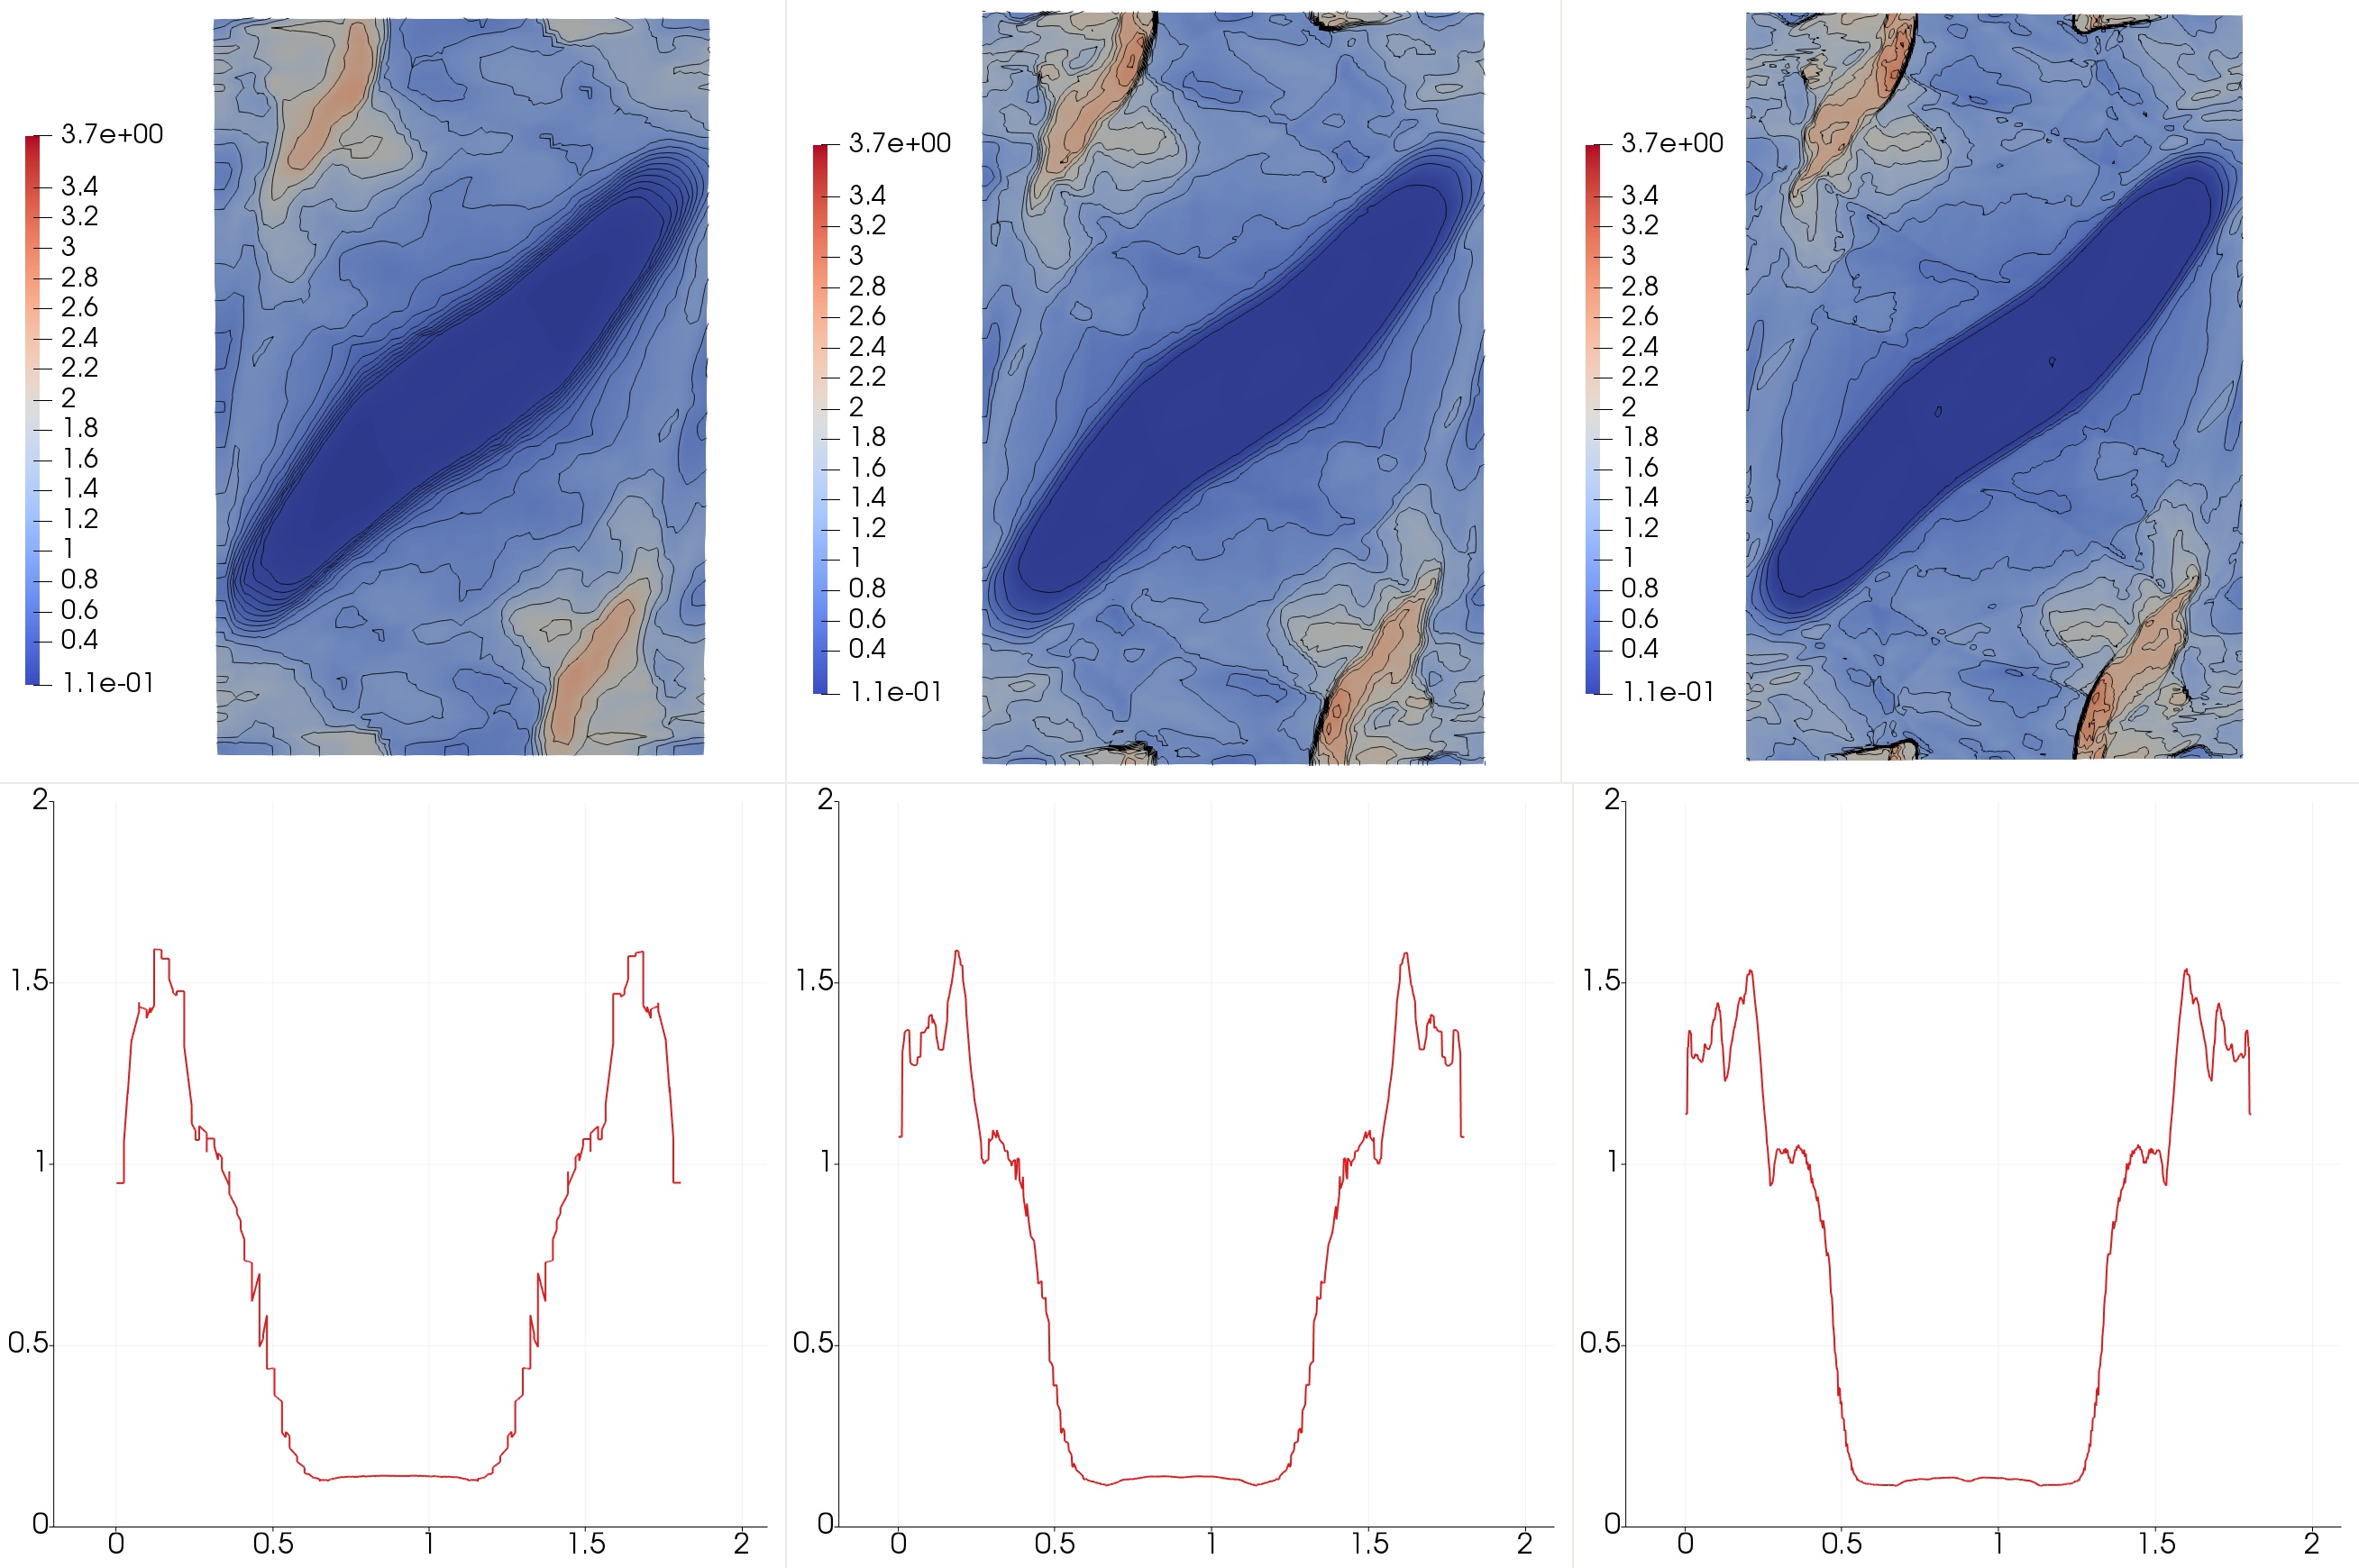
\includegraphics[width=0.92\textwidth]{img/mhd-blast/new/blast,1noadapt18.jpg}
		\caption{Fine solution on mesh }
	\label{figure:amrRef1}
	\end{center}
\end{figure}
\vspace{-4mm}


TODO - add outputs (Hermes / deal)
TODO - ukazat na 2d prikladu z Hermesu co to je referencni reseni, co to je ||zprojektovane - presne|| (v dealu?), co to je tohle bez normy, zminka o distribuovanosti, ze musim napocitat nejaky thresholdy mapReducem, atd.



\chapter{Results}
In this section, results from the computation using the implemented software are presented. There are two classical benchmarks for 3-dimensional MHD equations, namely the MHD Blast \cite{blast1}, \cite{blast2}, and the Orszag-Tang vortex \cite{vortex}. And then the main section of this work contains results from the flux tube eruption model on and above the Sun's surface.
\paragraph{}
In most cases, we are interested in the distribution of plasma density $\rho$ and the magnetic field $B$ in the domain $\Omega$.

\section{Benchmarks}
\label{sec:benchmarks}
The benchmarks presented in this Section do not have an exact analytical solution, but the formation of waves and discontinuities is well studied, and benchmarking is usually performed on the basis of comparing the structure and presence of non-physical attributes.
\subsection{Hardware specification}
For all following benchmarks, the setup described below was used. The computational mesh $T_h$ was formed in all cases by rectangular hexahedra.
The value of the time step $\tau$ used was set according to the CFL condition (\cref{section:CFL}).
The Taylor basis functions (see \cite{KuzminVertex}) and Divergence-free basis functions (\cref{tbl:divFreeBasis}) of order $0$ (piecewise constant functions) and $1$ (piecewise linear functions) were used.
Where appropriate (for piecewise linear basis functions), the slope limiting technique from \cref{sec:vertex} was used.
Illustration of the obtained results follows below - these results were obtained using one node of the department's computational cluster with these parameters:
\begin{itemize}
    \item CPU: Intel(R) Xeon(R) CPU E5-2680 v3 @ 2.50GHz,
    \item \# of Cores: 48 per node (nodes 1, 2), 16 per node (nodes 3, 4),
    \item RAM: 512 GB,
    \item C/C++ Compiler: GNU gcc 5.4.0,
		\item Vectorization support: AVX2,
    \item Parallelization implemented: Intel TBB,
    \item Distributed calculation implemented: OpenMPI.
\end{itemize}

\subsection{MHD Blast}
\subsubsection{MHD Blast - original version}
This benchmark has been used for decades - \cite{blast0}, \cite{blast1}, \cite{blast2} - in a variety of configurations and as a benchmark in software - e.g. \citep{athena}. The setup as described in \cite{blast0}, \cite{blast1} is defined (although in \cite{blast1} with interchanged $x-$ and $y-$ coordinates) by the initial conditions:
\begin{align}
\label{mhdBlastOld}
\gamma & =  5 / 3\\ \nonumber
p_0\lo\bfx, t\ro & =  100\ \ \text{for}\ \left|\bfx\right| < 0.1\\ \nonumber
p_0\lo\bfx, t\ro & =  1\ \ \text{for}\ \left|\bfx\right| \geq 0.1\\ \nonumber
\rho\lo\bfx, t = 0\ro & =  1,\\ \nonumber
p\lo\bfx, t = 0\ro & =  p_0\lo\bfx, t\ro,\\ \nonumber
\bfu_1\lo\bfx, t = 0\ro & =  0,\\ \nonumber
\bfu_2\lo\bfx, t = 0\ro & =  0,\\ \nonumber
\bfu_3\lo\bfx, t = 0\ro & =  0,\\ \nonumber
\bfB_1\lo\bfx, t = 0\ro & =  0,\\ \nonumber
\bfB_2\lo\bfx, t = 0\ro & =  100,\\ \nonumber
\bfB_3\lo\bfx, t = 0\ro & =  0.
\end{align}
Total energy is calculated using \cref{magU,kinU,presU}.
The domain $\Omega$ is a square, with scaling quite arbitrarily used in the papers. In the case of \cite{blast1}, $\Omega = [0, 1] \times [0, 1]$, in this work it is $\Omega = [-0.5, 0.5] \times [-0.5, 0.5]$.

It is obvious from the initial setup, that the example is true to its name, and it is in fact a blast of the over-pressured area $\left|\bfx\right| < 0.1$, where pressure $p$ is 100$\times$ larger than elsewhere in the domain. This setup is completed with simple outflow boundary condition \cref{bcoutdef}.
In the next figures, the solution as presented in \cite{blast1} is compared to the solution obtained with the approach described in this work. Note that the solution from \cite{blast1} needed to have the axes transformed $\lo x\rightleftharpoons y\ro$ with respect to the original paper. The \cref{figure:blastOldRef} is taken from the article \cite{blast1} from the page 33. Unfortunately the paper does not specify the precise time at which the snapshots are taken.

\begin{figure}[H]
\centering
\hspace{-8mm}
\begin{subfigure}[b]{0.4\textwidth}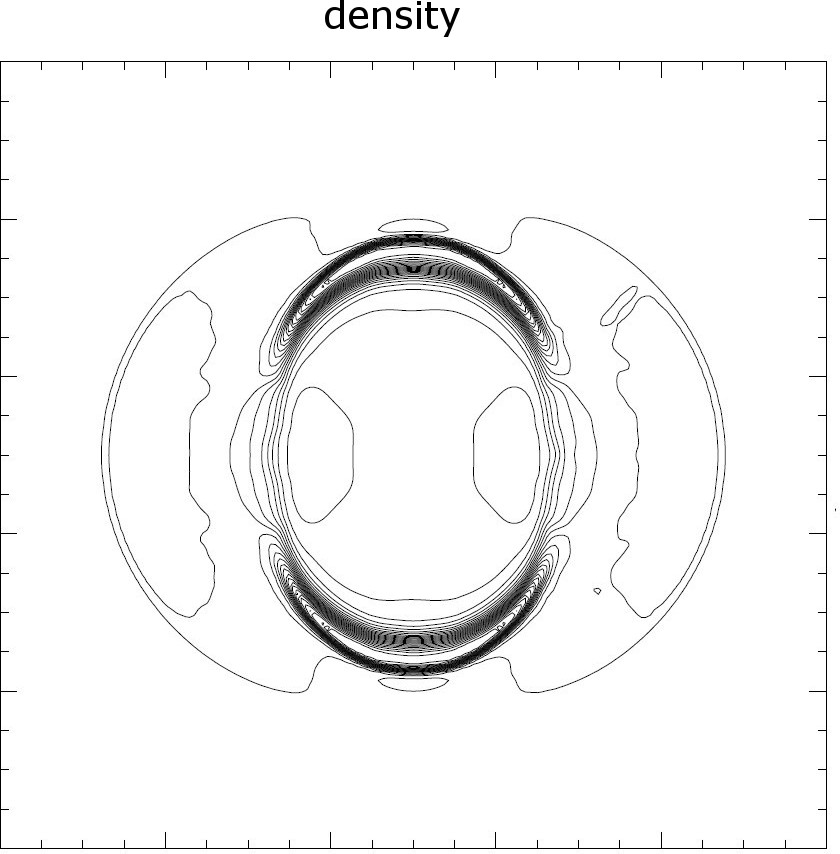
\includegraphics[width=\textwidth]{img/mhd-blast/old/ref.jpg}\end{subfigure}
\begin{subfigure}[b]{0.395\textwidth}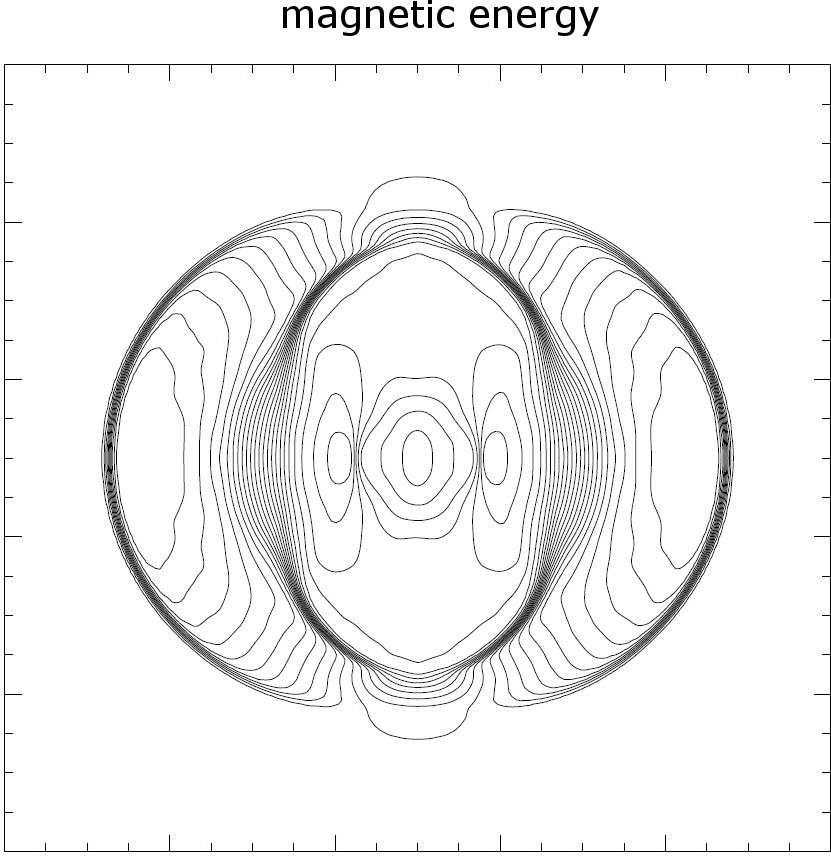
\includegraphics[width=\textwidth]{img/mhd-blast/old/refmag.jpg}\end{subfigure}
\caption{Results from \cite{blast1}, density(left), magnetic energy(right)}
\label{figure:blastOldRef}
\end{figure}

\vspace{-5mm}
\begin{figure}[H]
	\begin{center}
		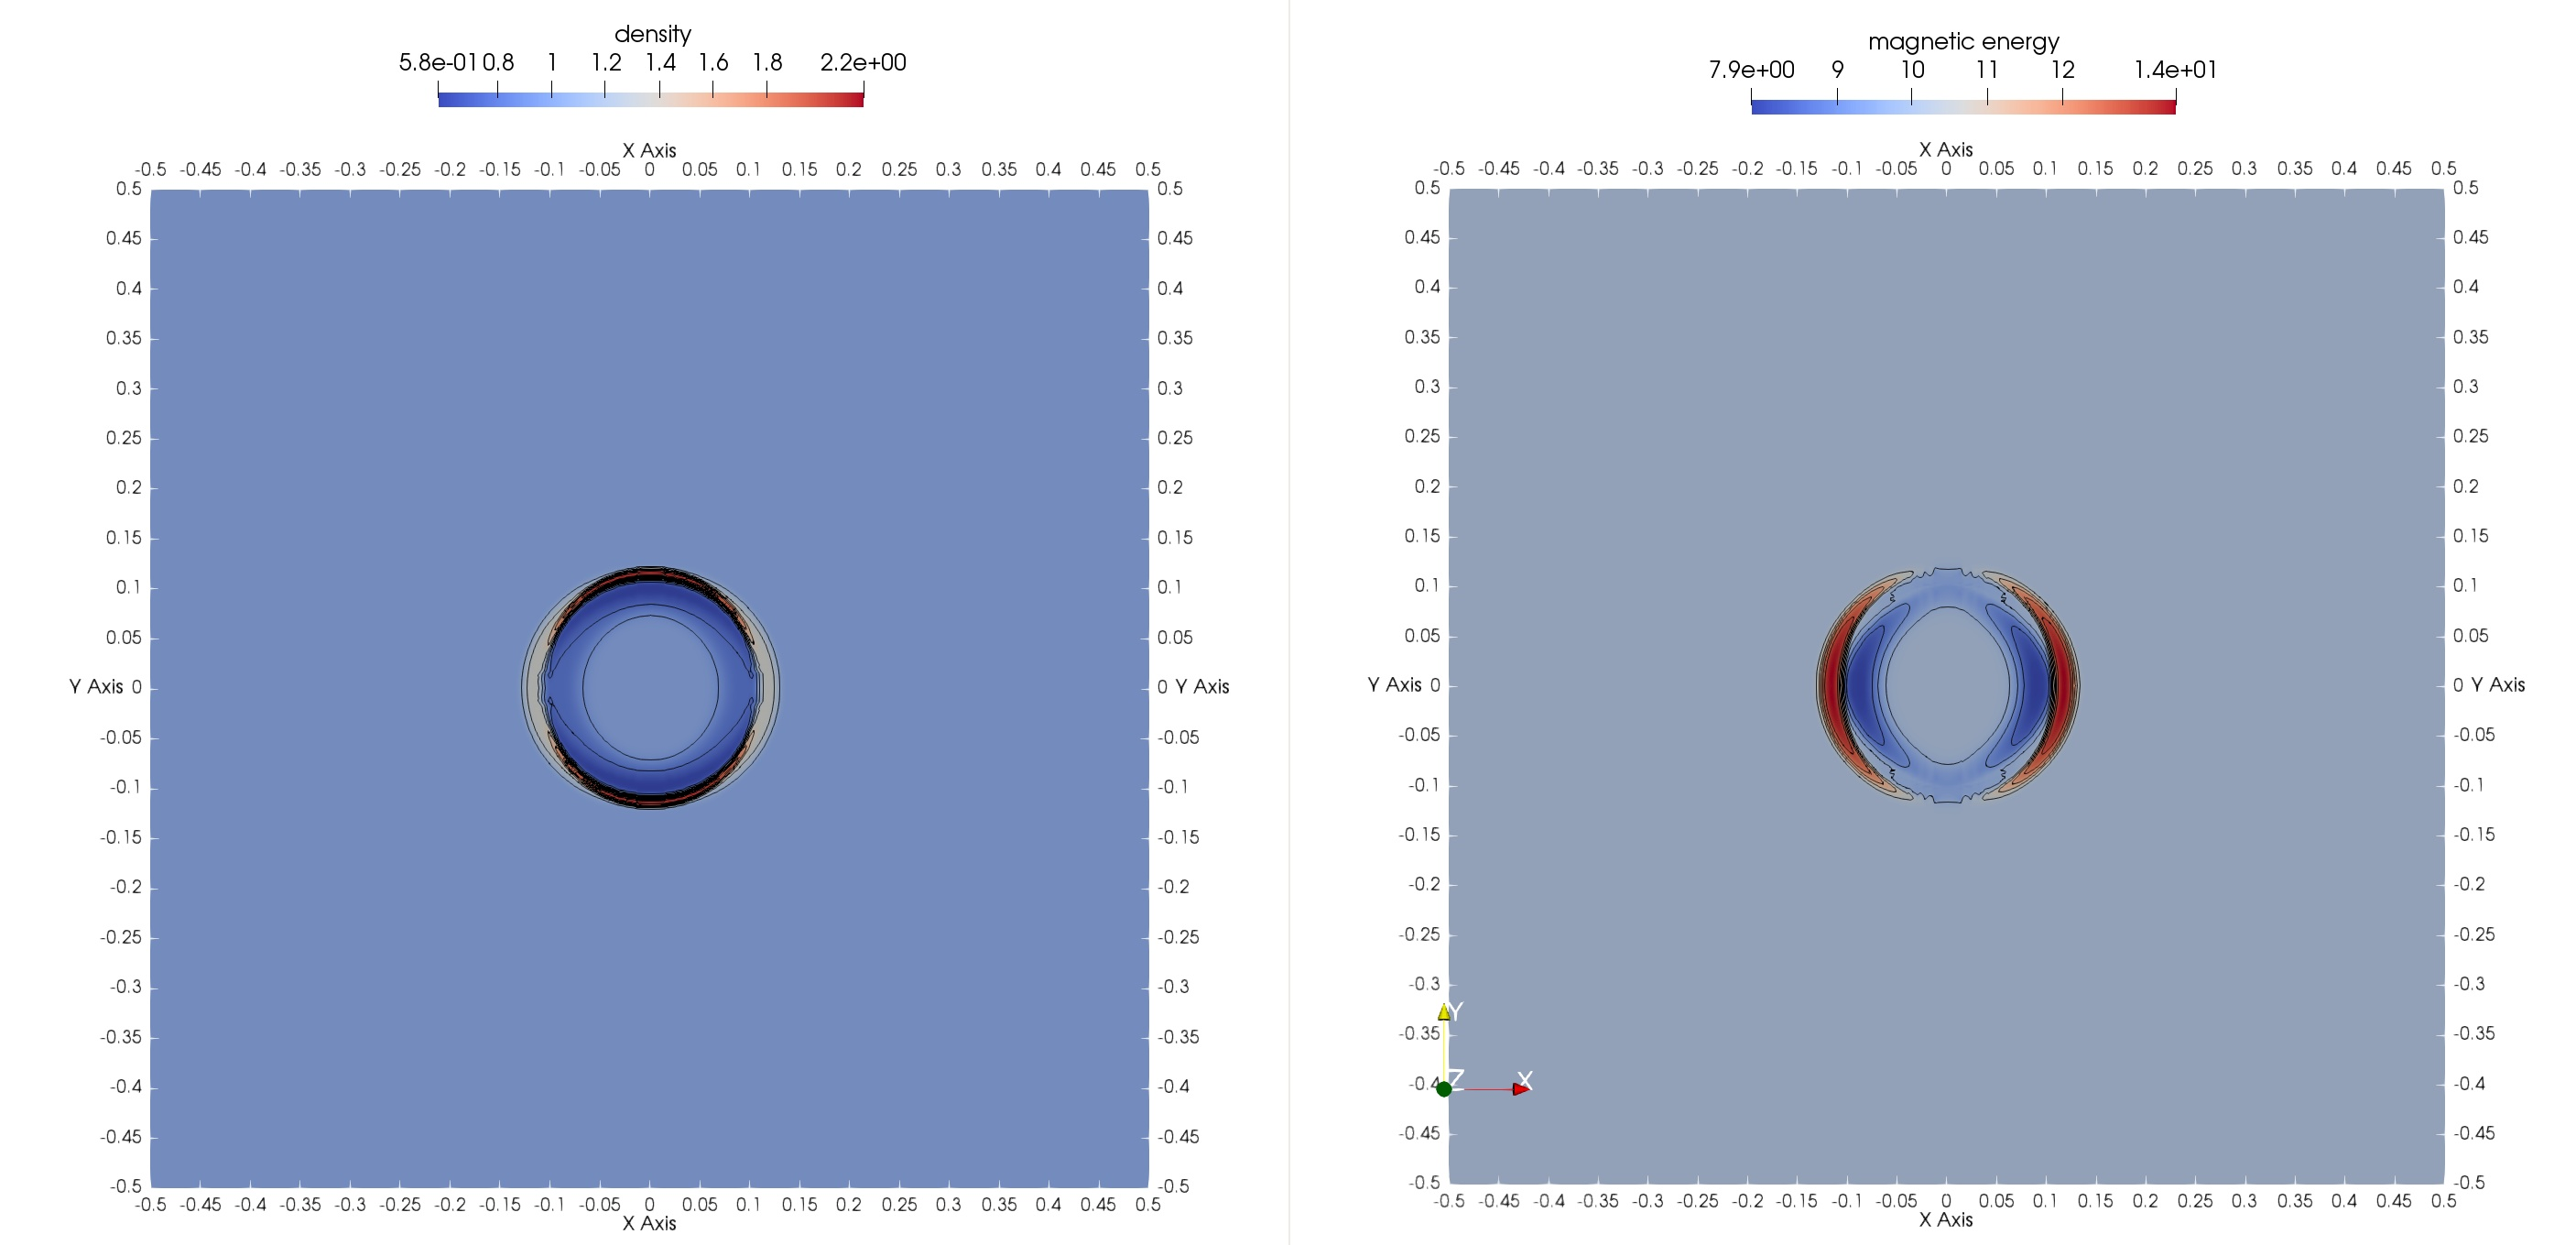
\includegraphics[width=0.93\textwidth]{img/mhd-blast/old/mynew1.jpg}
	\caption{Obtained results, $t = 10^{-3}$, density(left), magnetic energy(right)}
	\label{figure:blastOldMy1}
	\end{center}
\end{figure}
\vspace{-8mm}

\begin{figure}[H]
	\begin{center}
		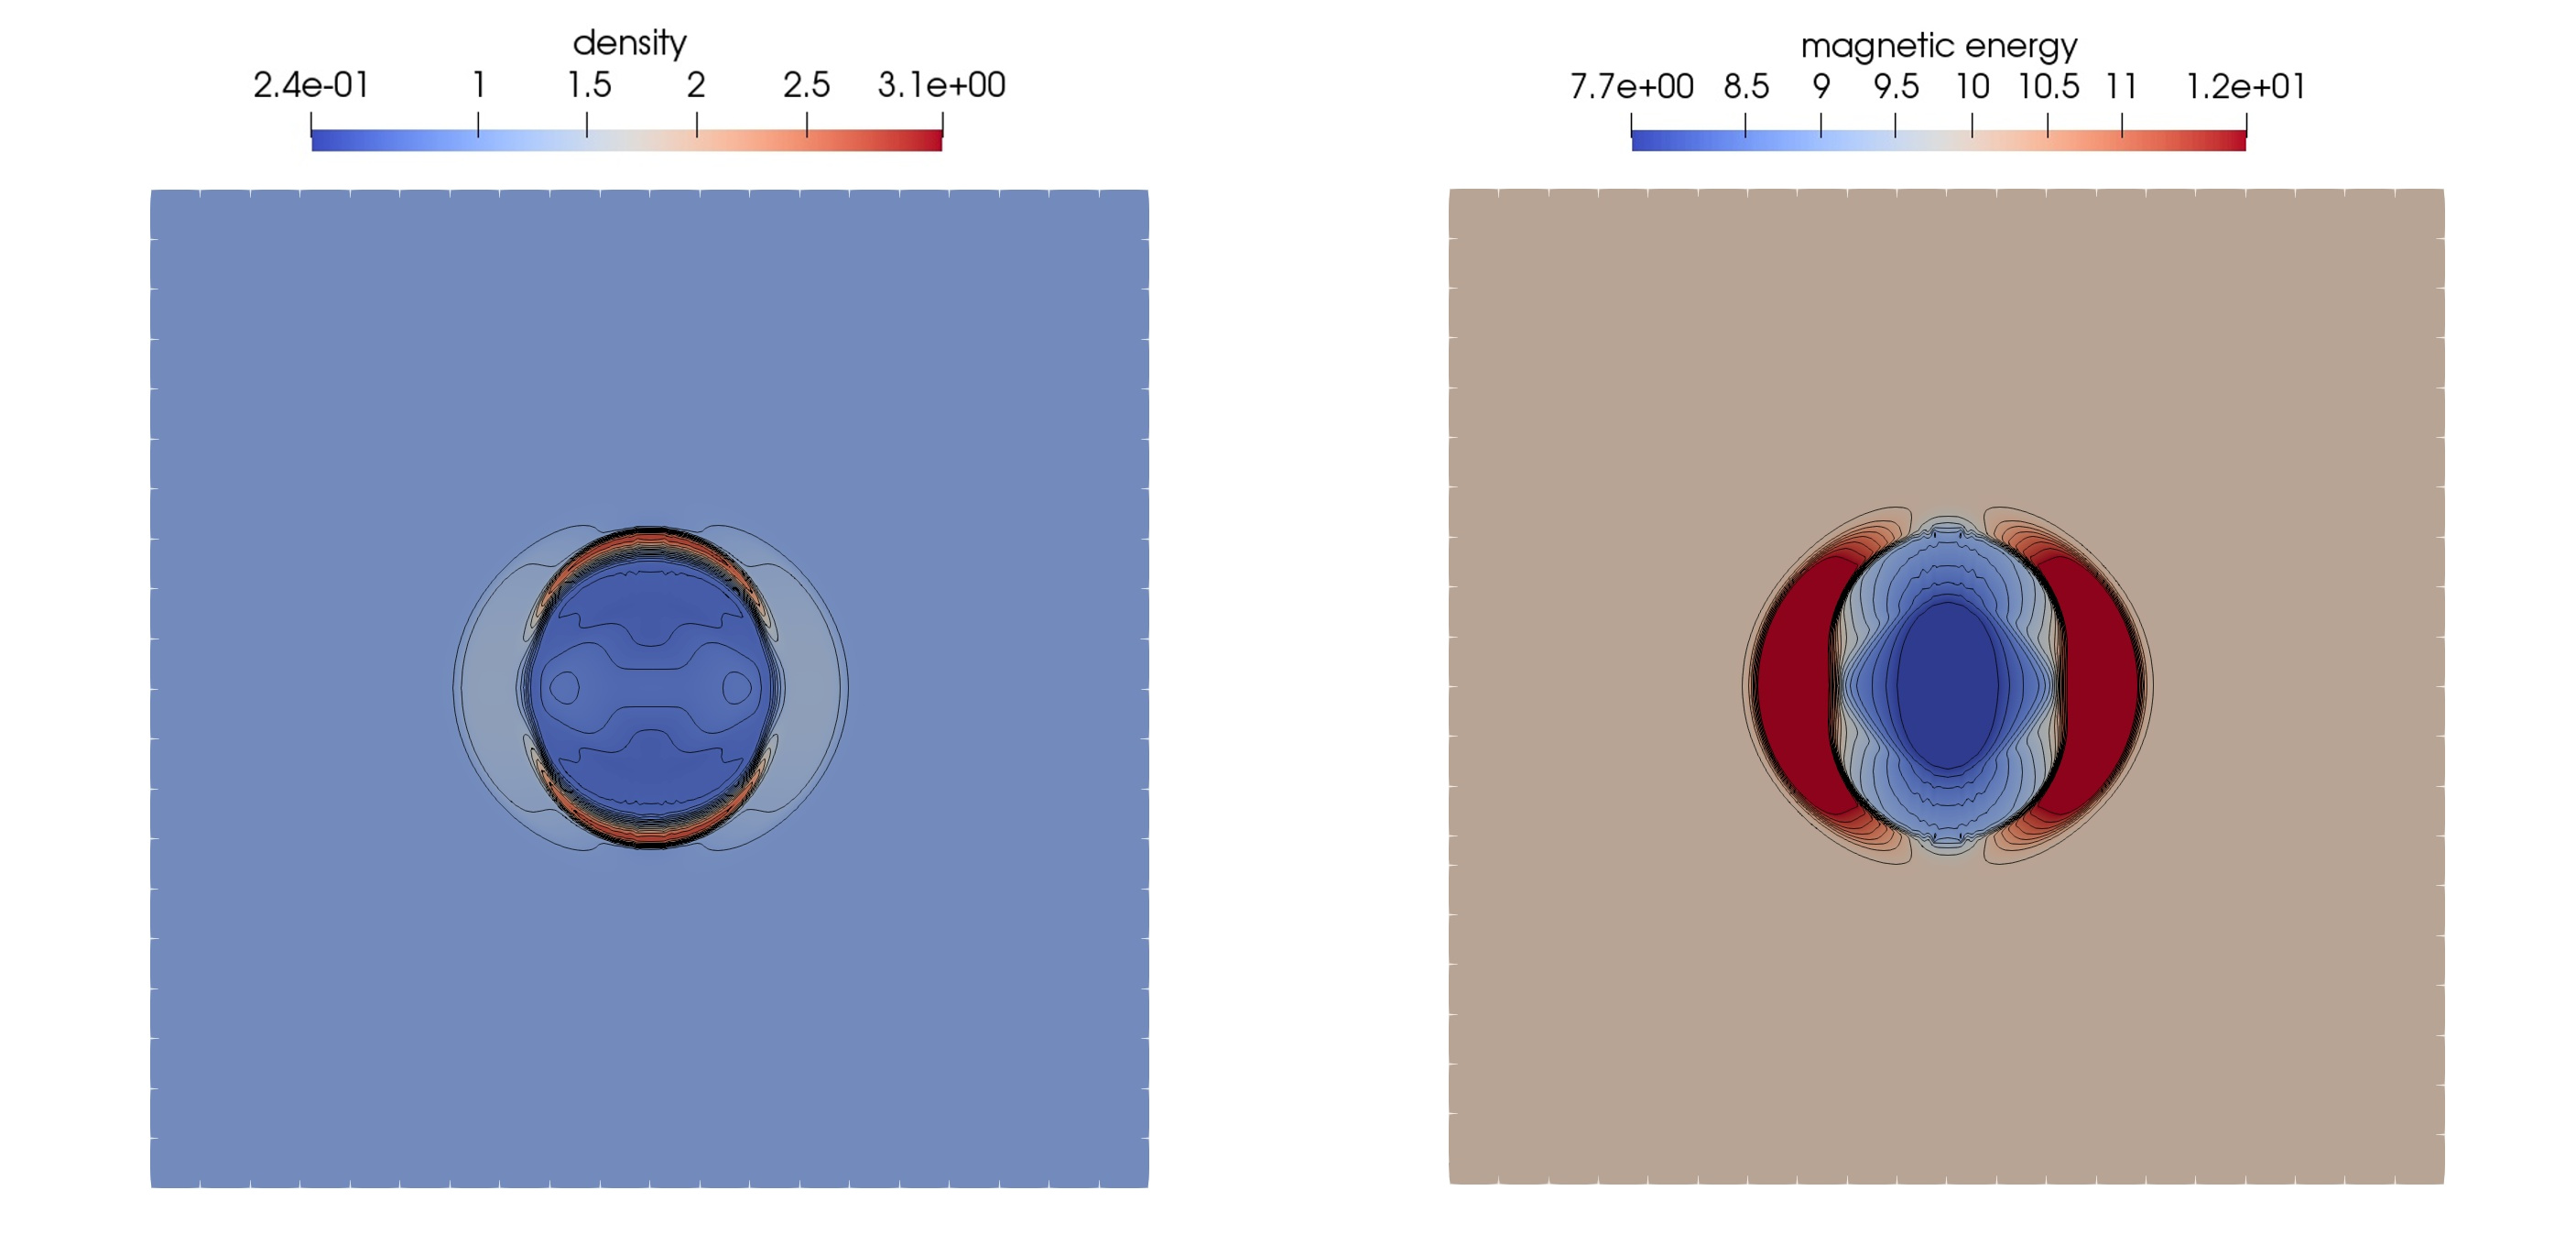
\includegraphics[width=0.93\textwidth]{img/mhd-blast/old/mynew2.jpg}
	\caption{Obtained results, $t = 6\cdot 10^{-3}$, density(left), magnetic energy(right)}
	\label{figure:blastOldMy2}
	\end{center}
\end{figure}
\vspace{-8mm}

\begin{figure}[H]
	\begin{center}
		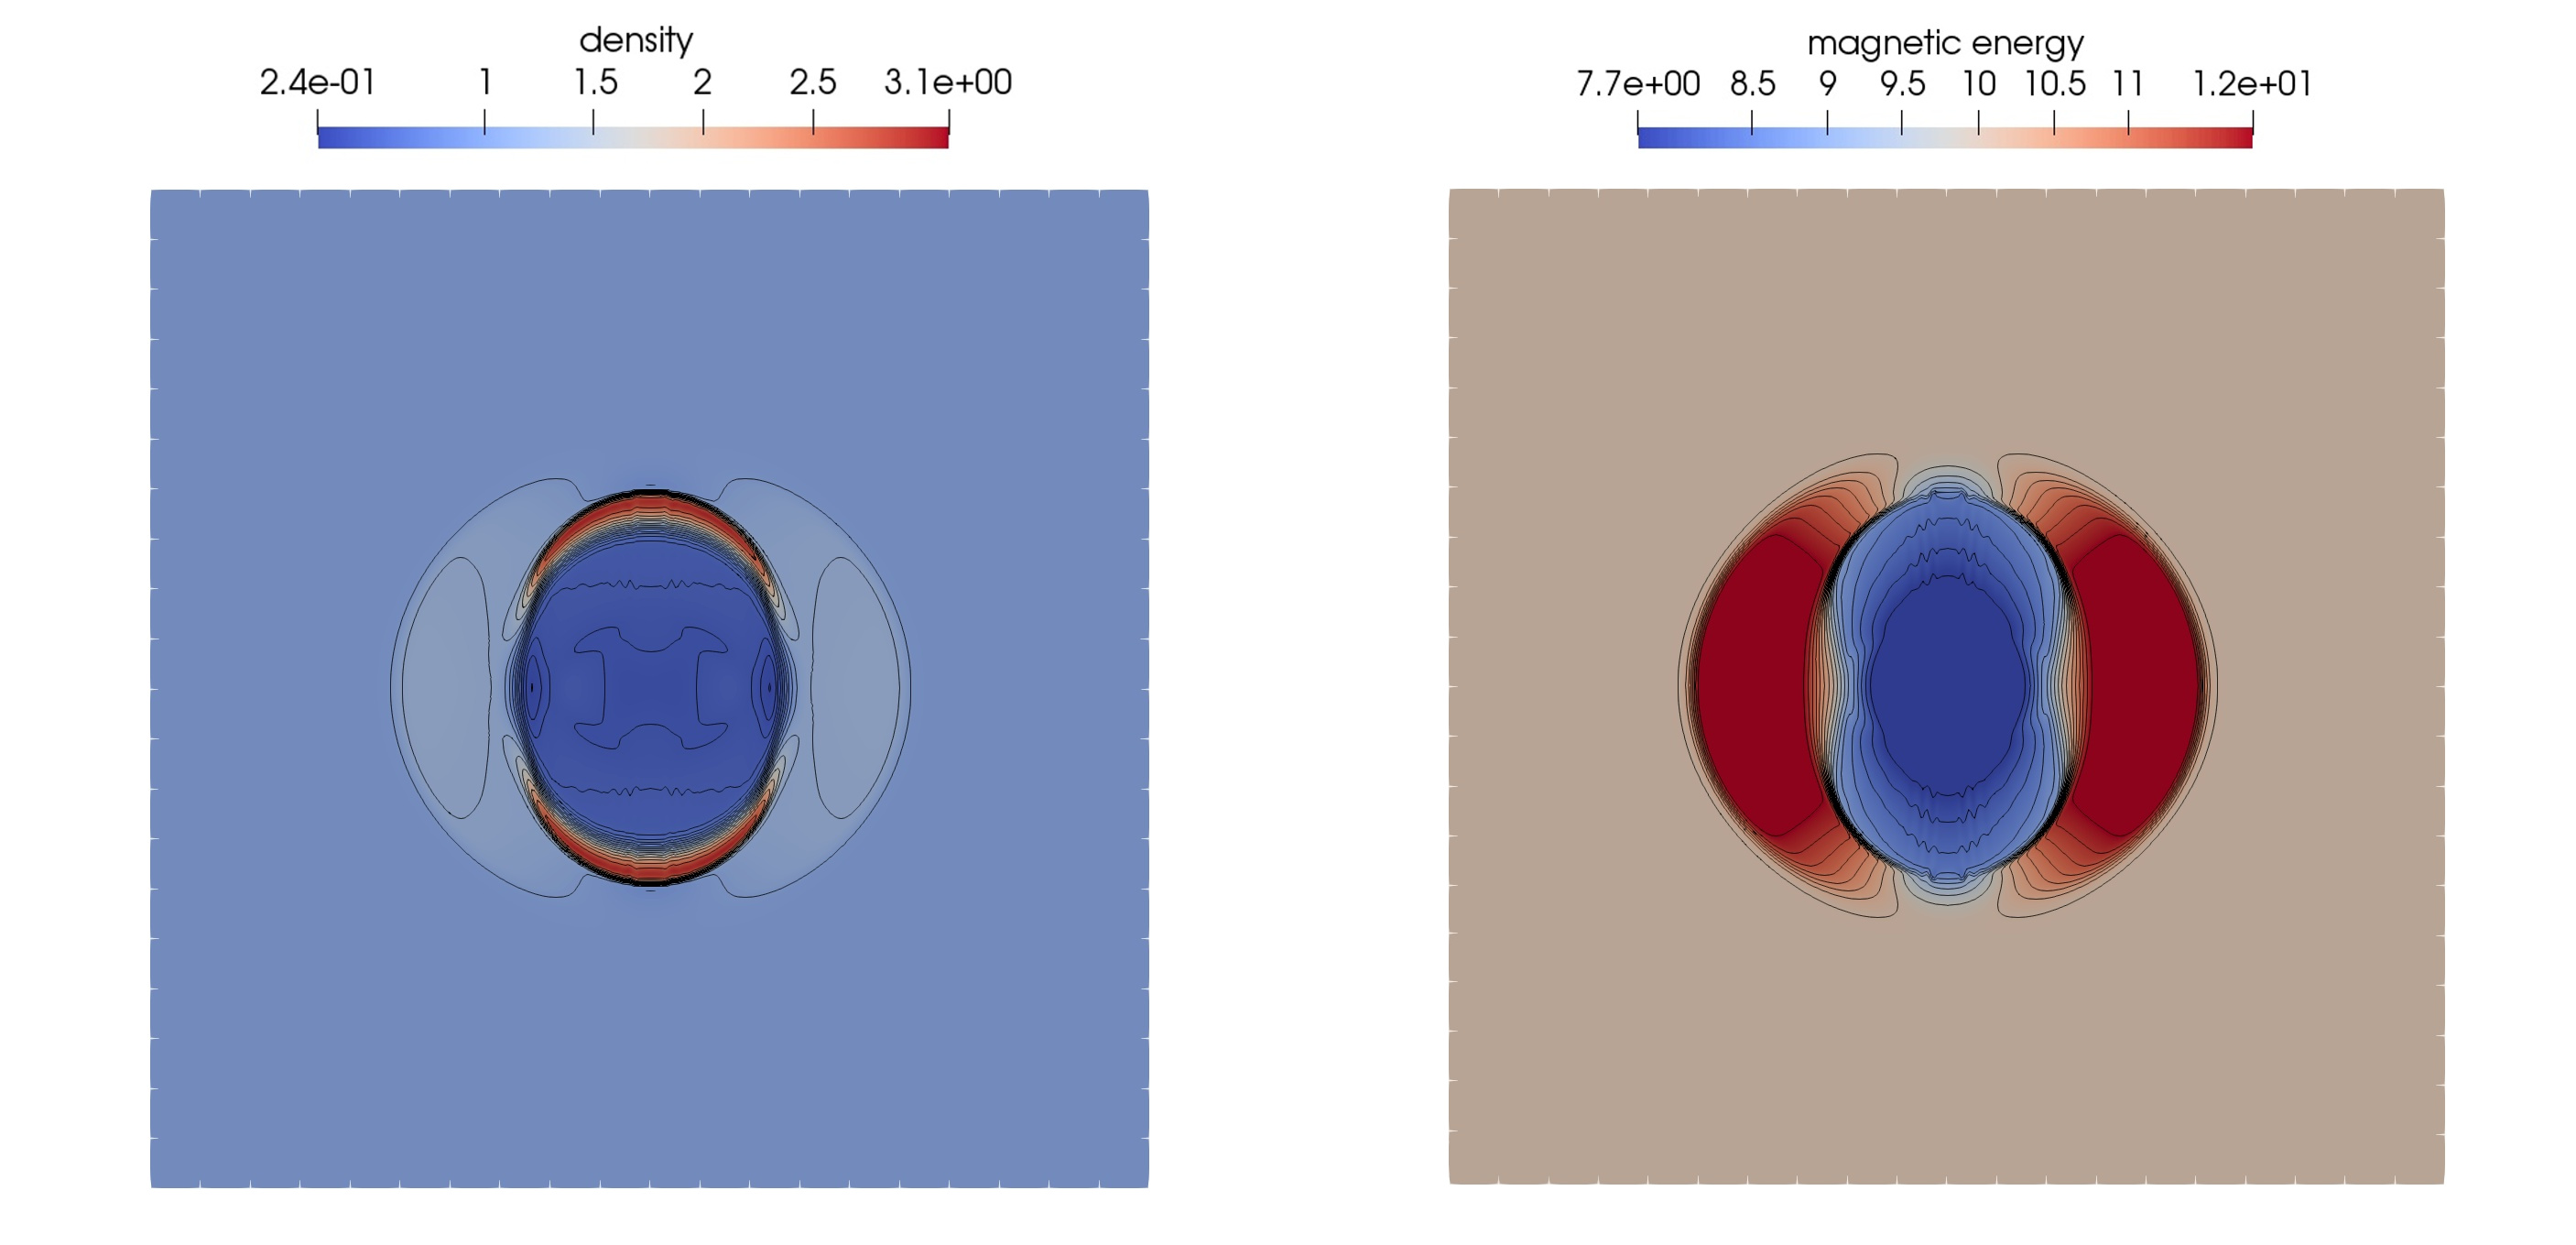
\includegraphics[width=0.93\textwidth]{img/mhd-blast/old/mynew3.jpg}
	\caption{Obtained results, $t = 11\cdot 10^{-3}$, density(left), magnetic energy(right)}
	\label{figure:blastOldMy3}
	\end{center}
\end{figure}
\vspace{-8mm}

\begin{figure}[H]
	\begin{center}
		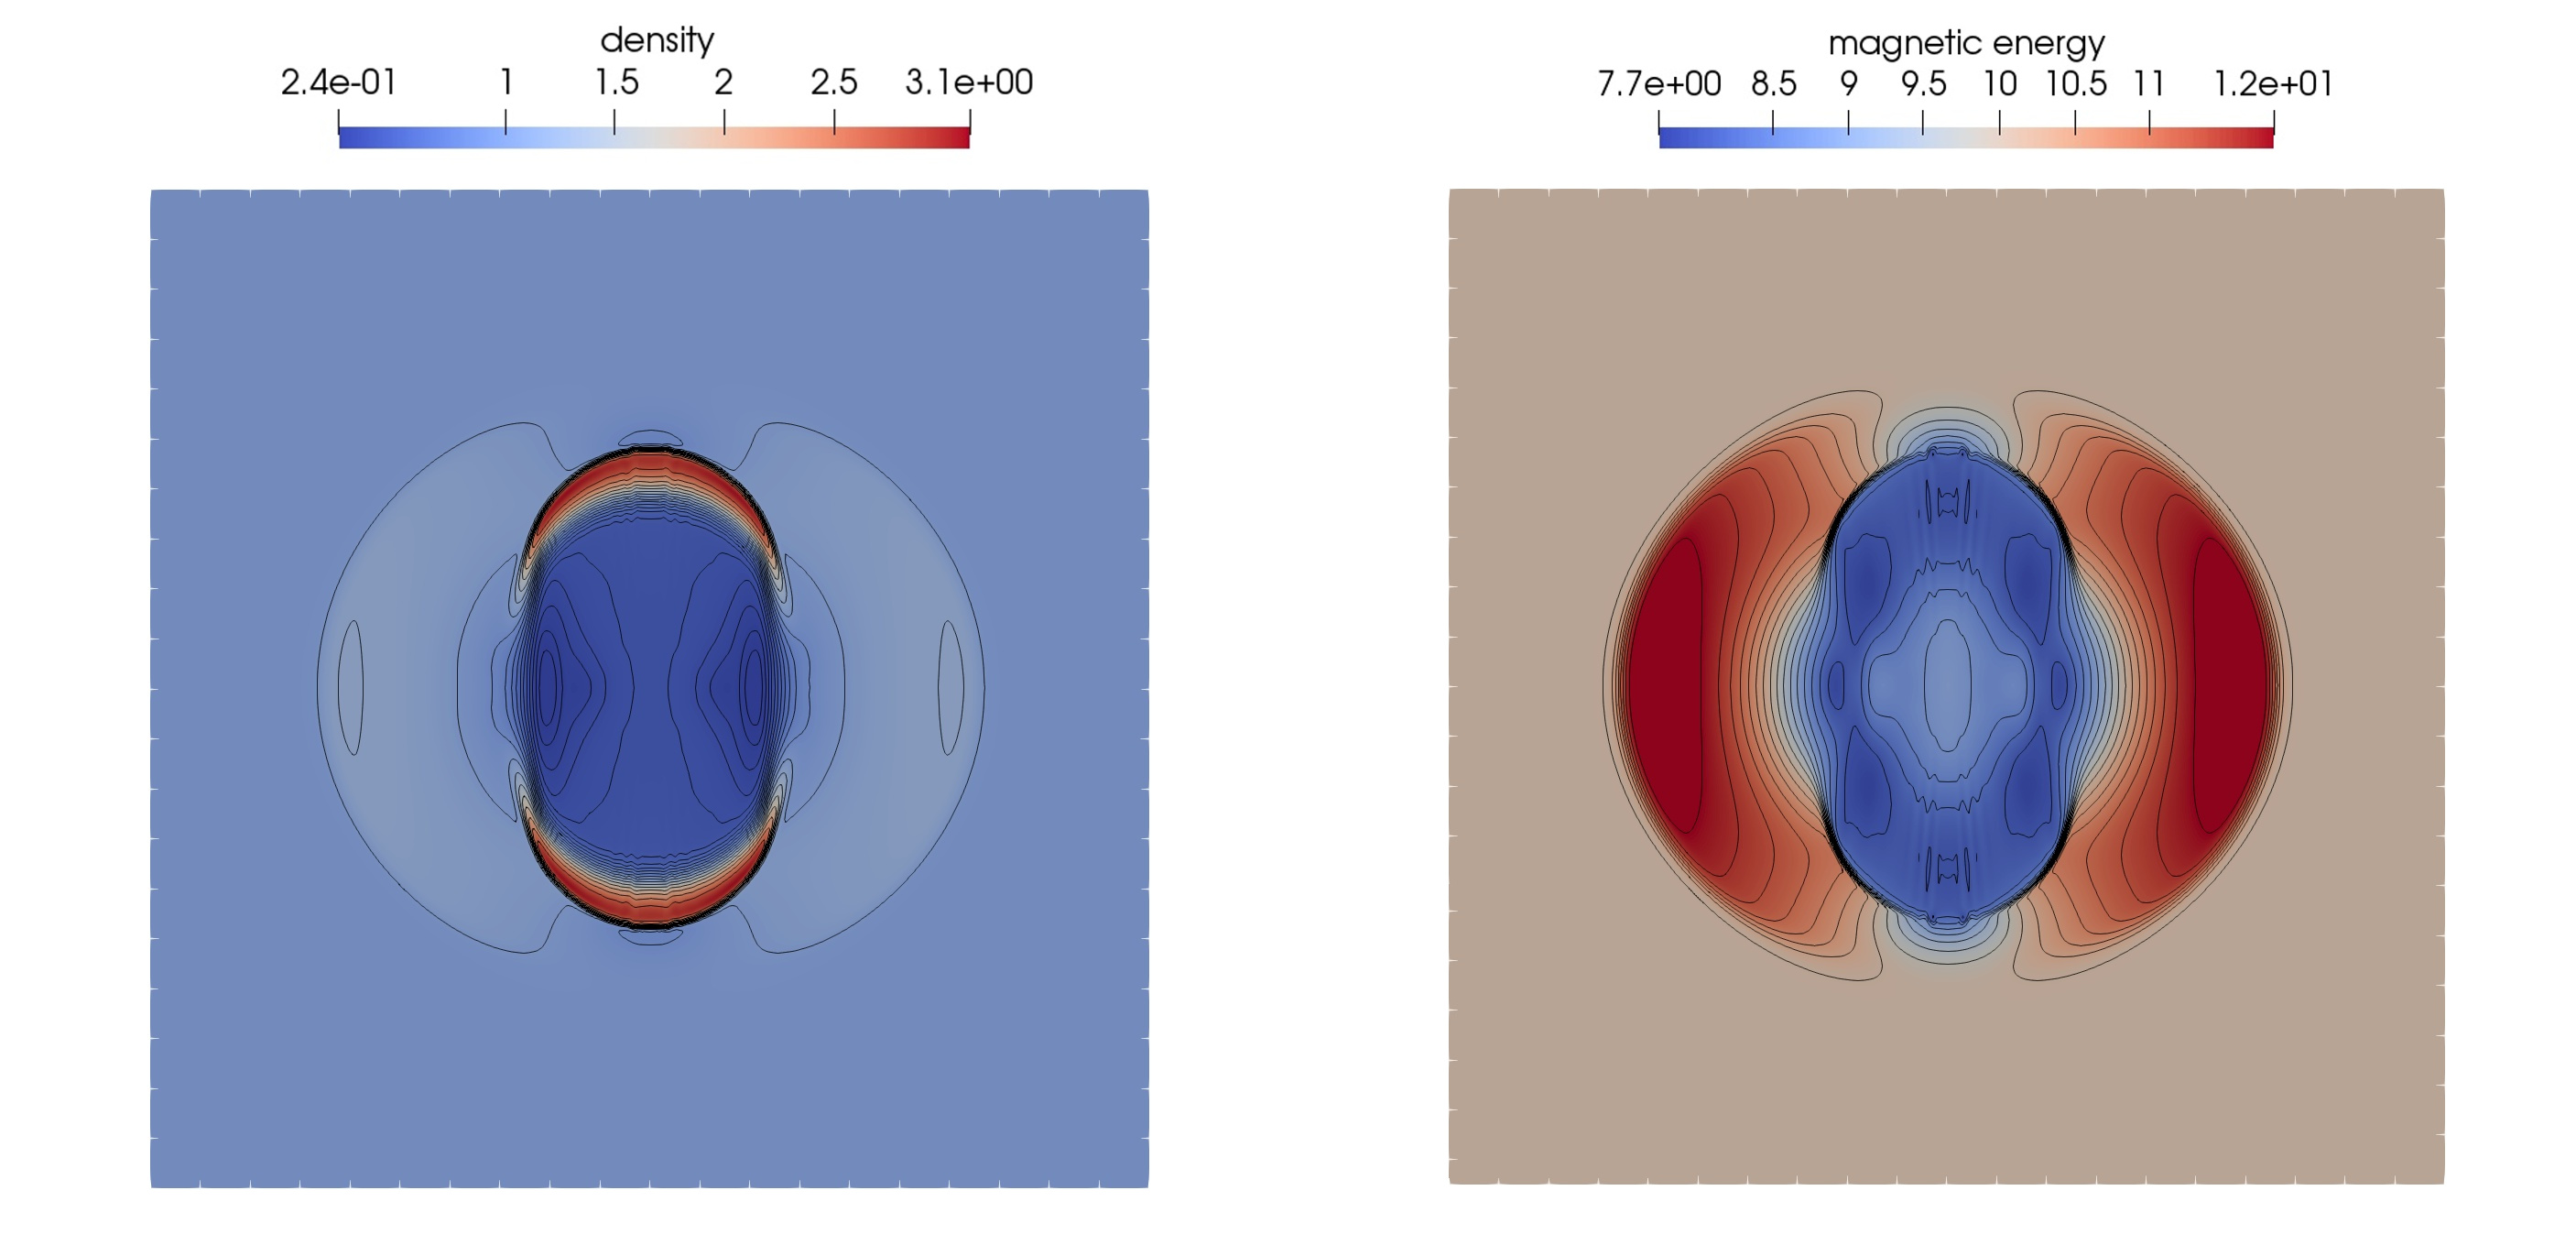
\includegraphics[width=0.93\textwidth]{img/mhd-blast/old/mynew4.jpg}
	\caption{Obtained results, $t = 16\cdot 10^{-3}$, density(left), magnetic energy(right)}
	\label{figure:blastOldMy4}
	\end{center}
\end{figure}
\vspace{-8mm}

\begin{figure}[H]
	\begin{center}
		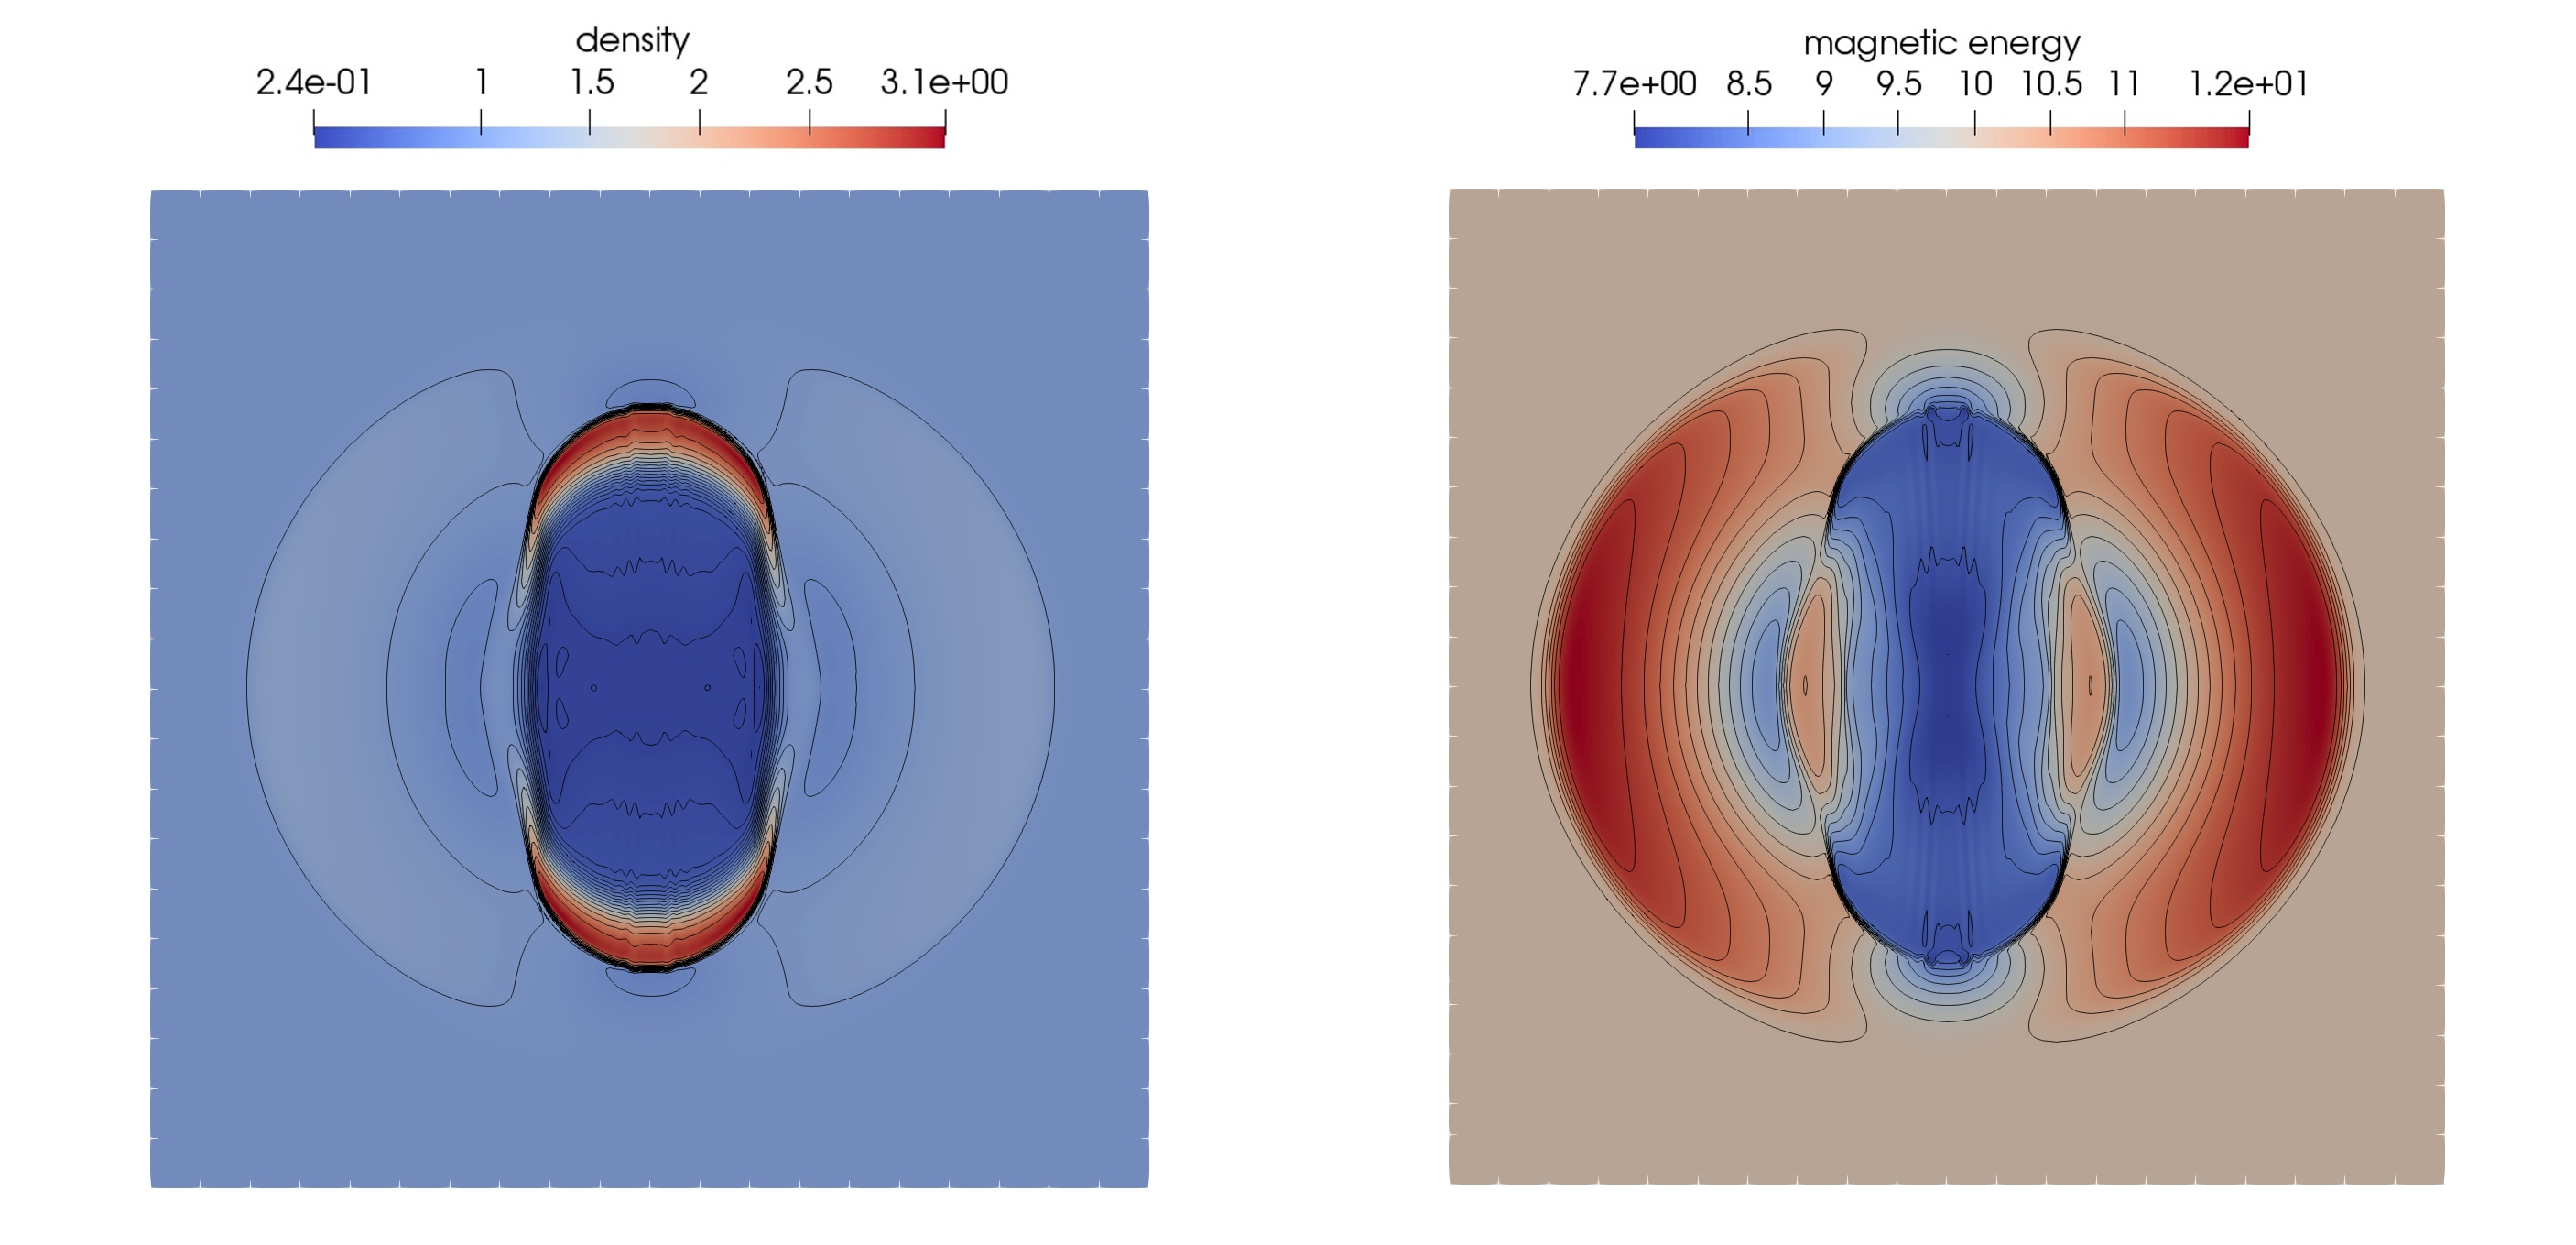
\includegraphics[width=0.93\textwidth]{img/mhd-blast/old/mynew5.jpg}
	\caption{Obtained results, $t = 23\cdot 10^{-3}$, density(left), magnetic energy(right)}
	\label{figure:blastOldMy5}
	\end{center}
\end{figure}
\vspace{-5mm}
The solution in \cref{figure:blastOldMy4,figure:blastOldMy5}  is apparently almost identical to that in \cref{figure:blastOldRef}. To demonstrate the distributed nature of the computation, in \cref{figure:subdomainsBlastOld}, color-mapping of elements $K \in T$ to processors owning the particular element is presented (see \cref{section:ditributedTria} for details). Note that there were $48$ processors used for the computation.

\begin{figure}[H]
	\begin{center}
		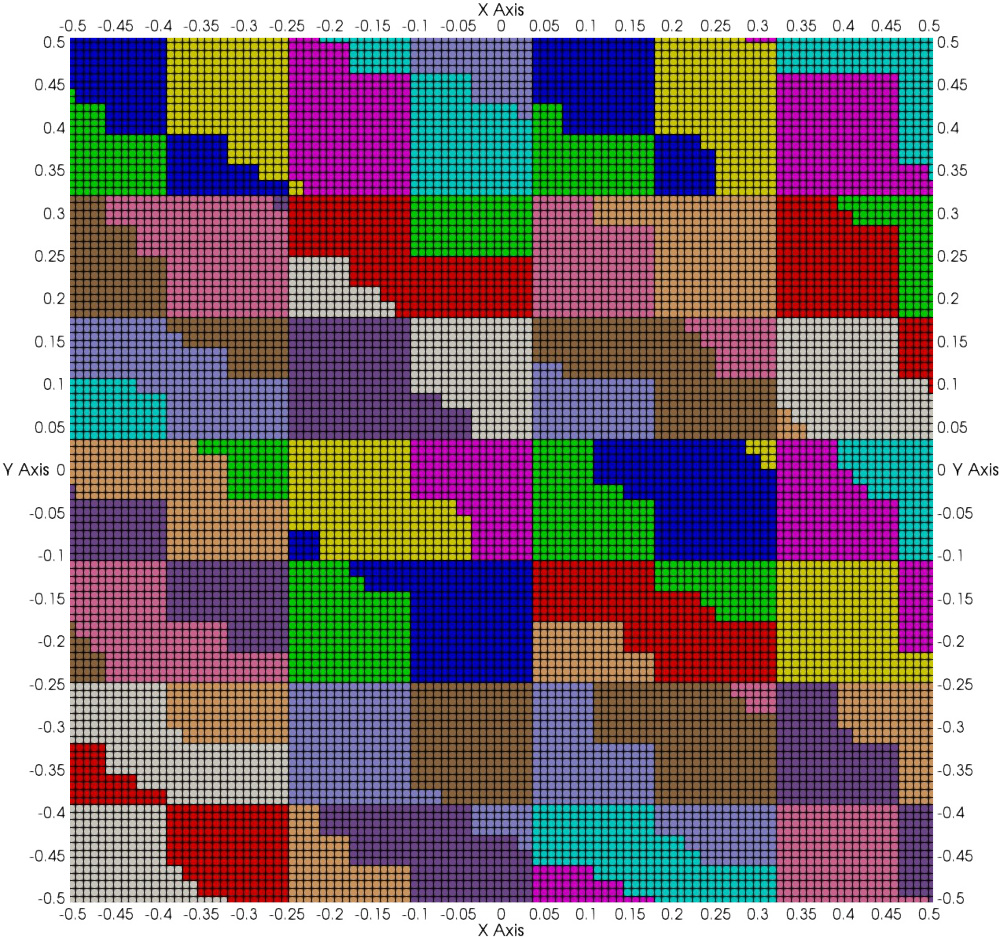
\includegraphics[width=0.75\textwidth]{img/mhd-blast/old/subdomain.jpg}
	\caption{Color-mapping of elements to processors for the computation of \crefrange{figure:blastOldMy1}{figure:blastOldMy5}}
	\label{figure:subdomainsBlastOld}
	\end{center}
\end{figure}
\vspace{-5mm}

This however, was a static calculation with 200 mesh elements in the $x-$ and $y-$ dimensions. In order to see how the AMR (see \cref{chapter:amr}) performs, the same computation was performed in adaptive setup. Starting from a very coarse mesh of 10 elements in both dimensions, the evolving mesh and its distribution to processors are shown in \crefrange{figure:blastOldMyAdapt1}{figure:blastOldMyAdapt6} - the distribution to processors on the left, the mesh elements on the right.

\begin{figure}[H]
	\begin{center}
		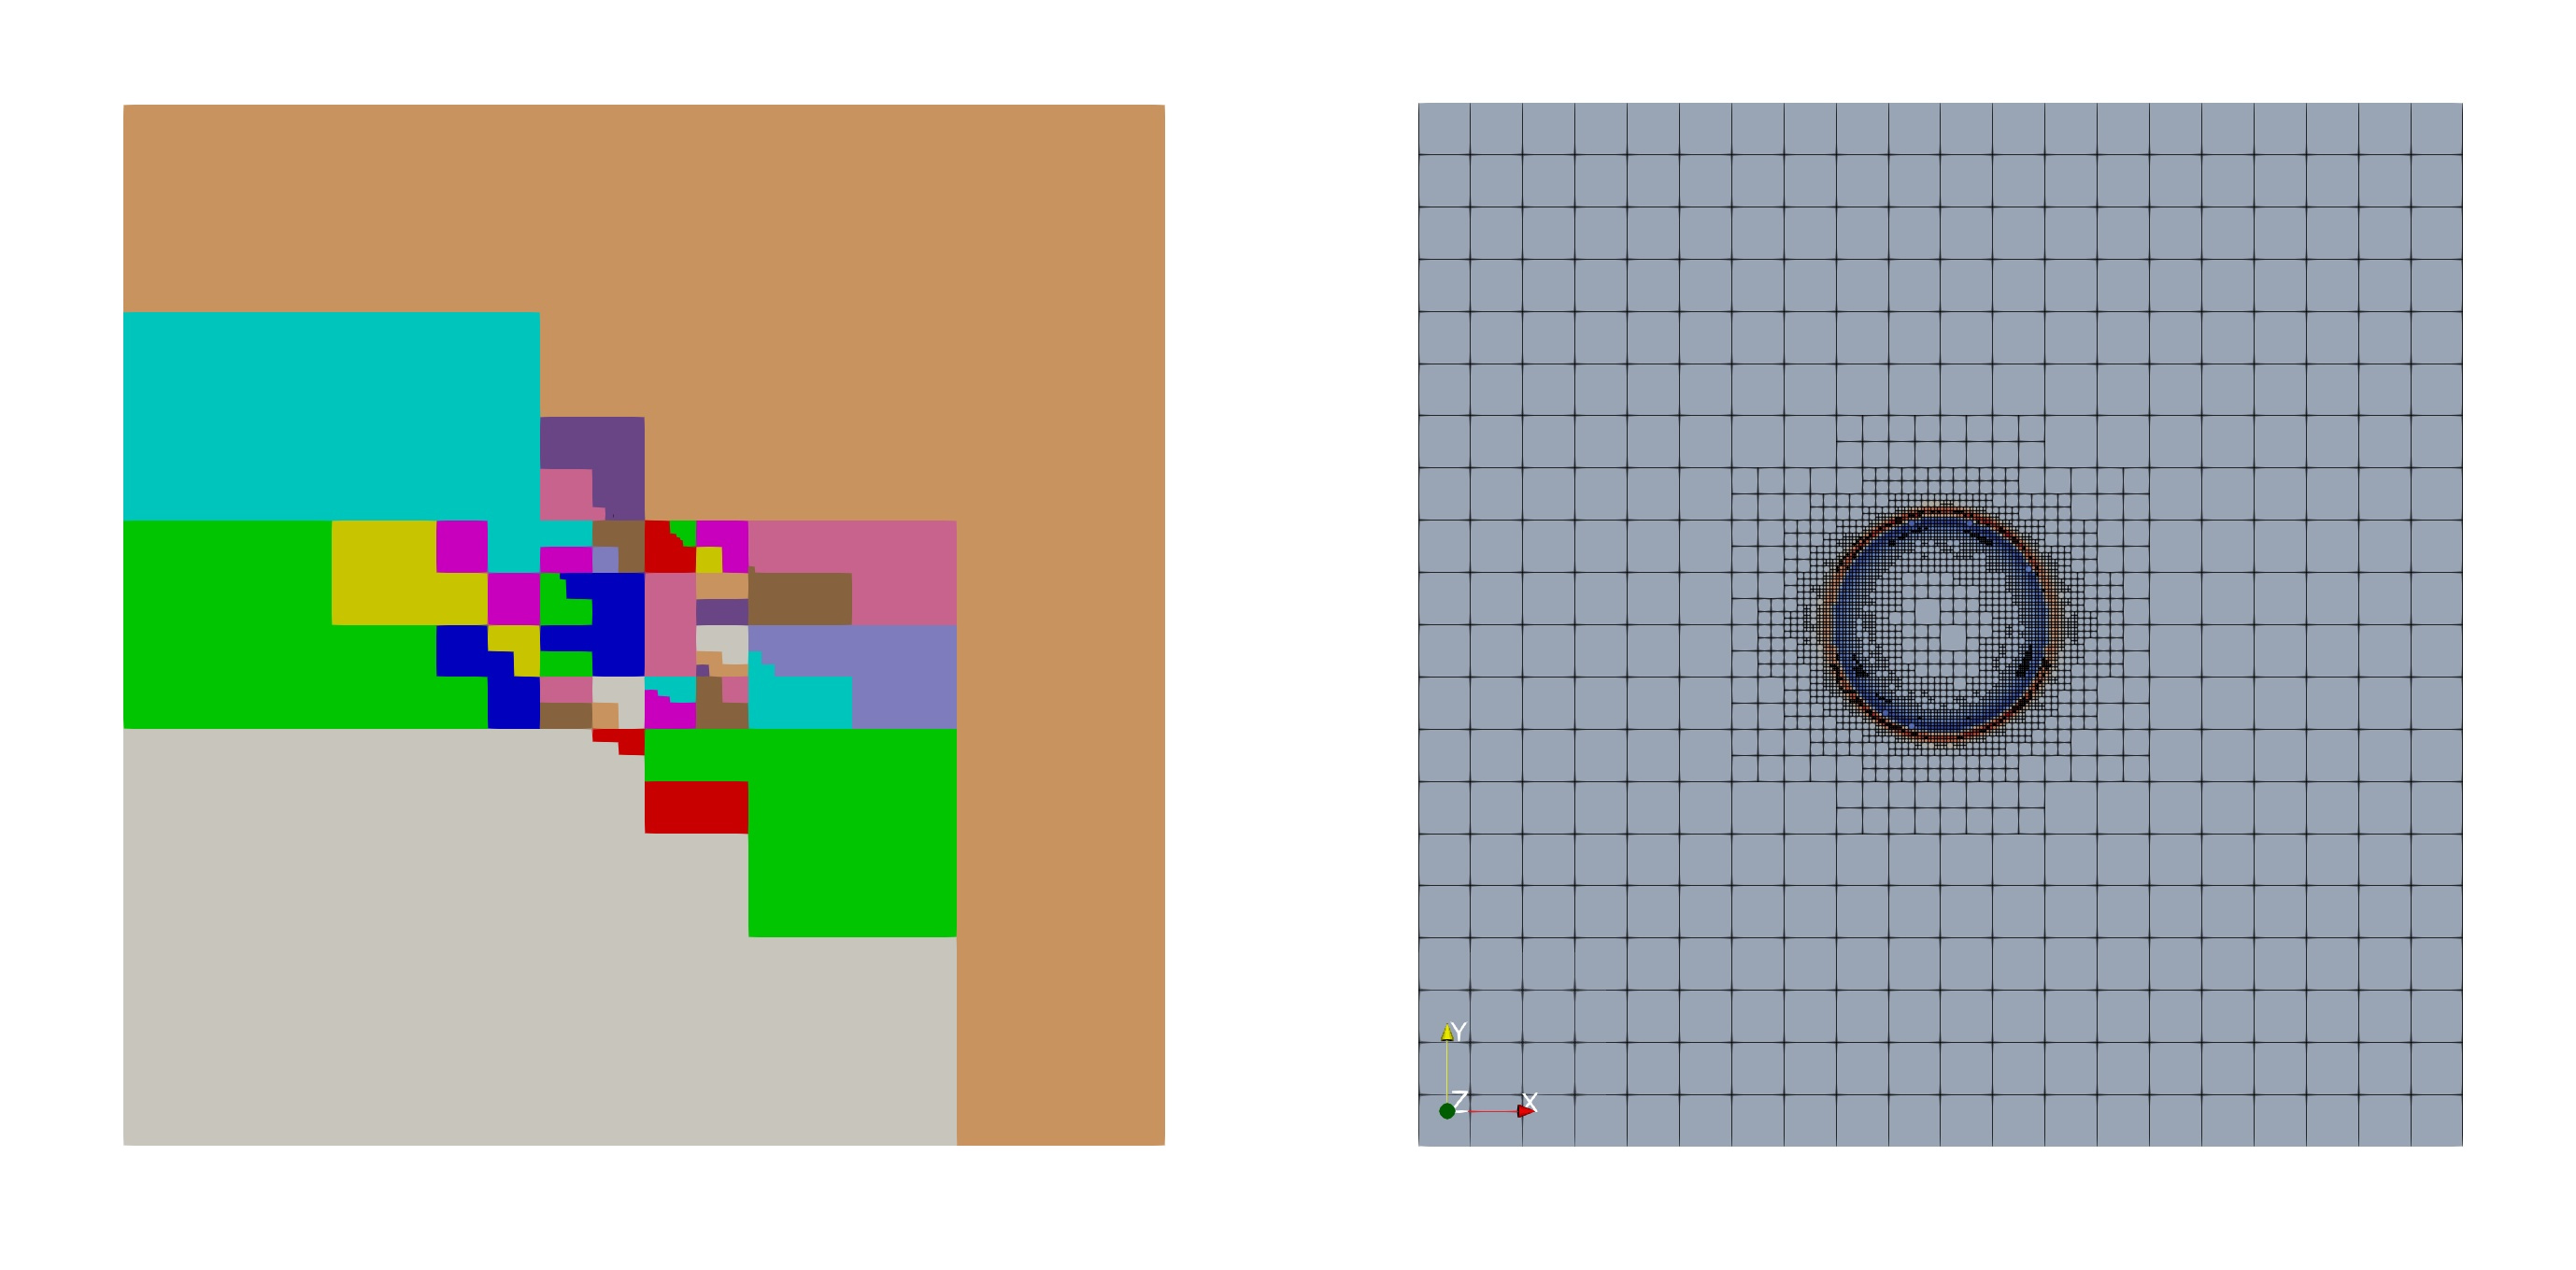
\includegraphics[width=0.87\textwidth]{img/mhd-blast/old/mya1.jpg}
	\caption{Obtained results, initial state, distribution of $\rho$ on elements in $T\lo\Omega\ro$ (right) and distribution of these elements to processors (left)}
	\label{figure:blastOldMyAdapt1}
	\end{center}
\end{figure}
\vspace{-8mm}

\begin{figure}[H]
	\begin{center}
		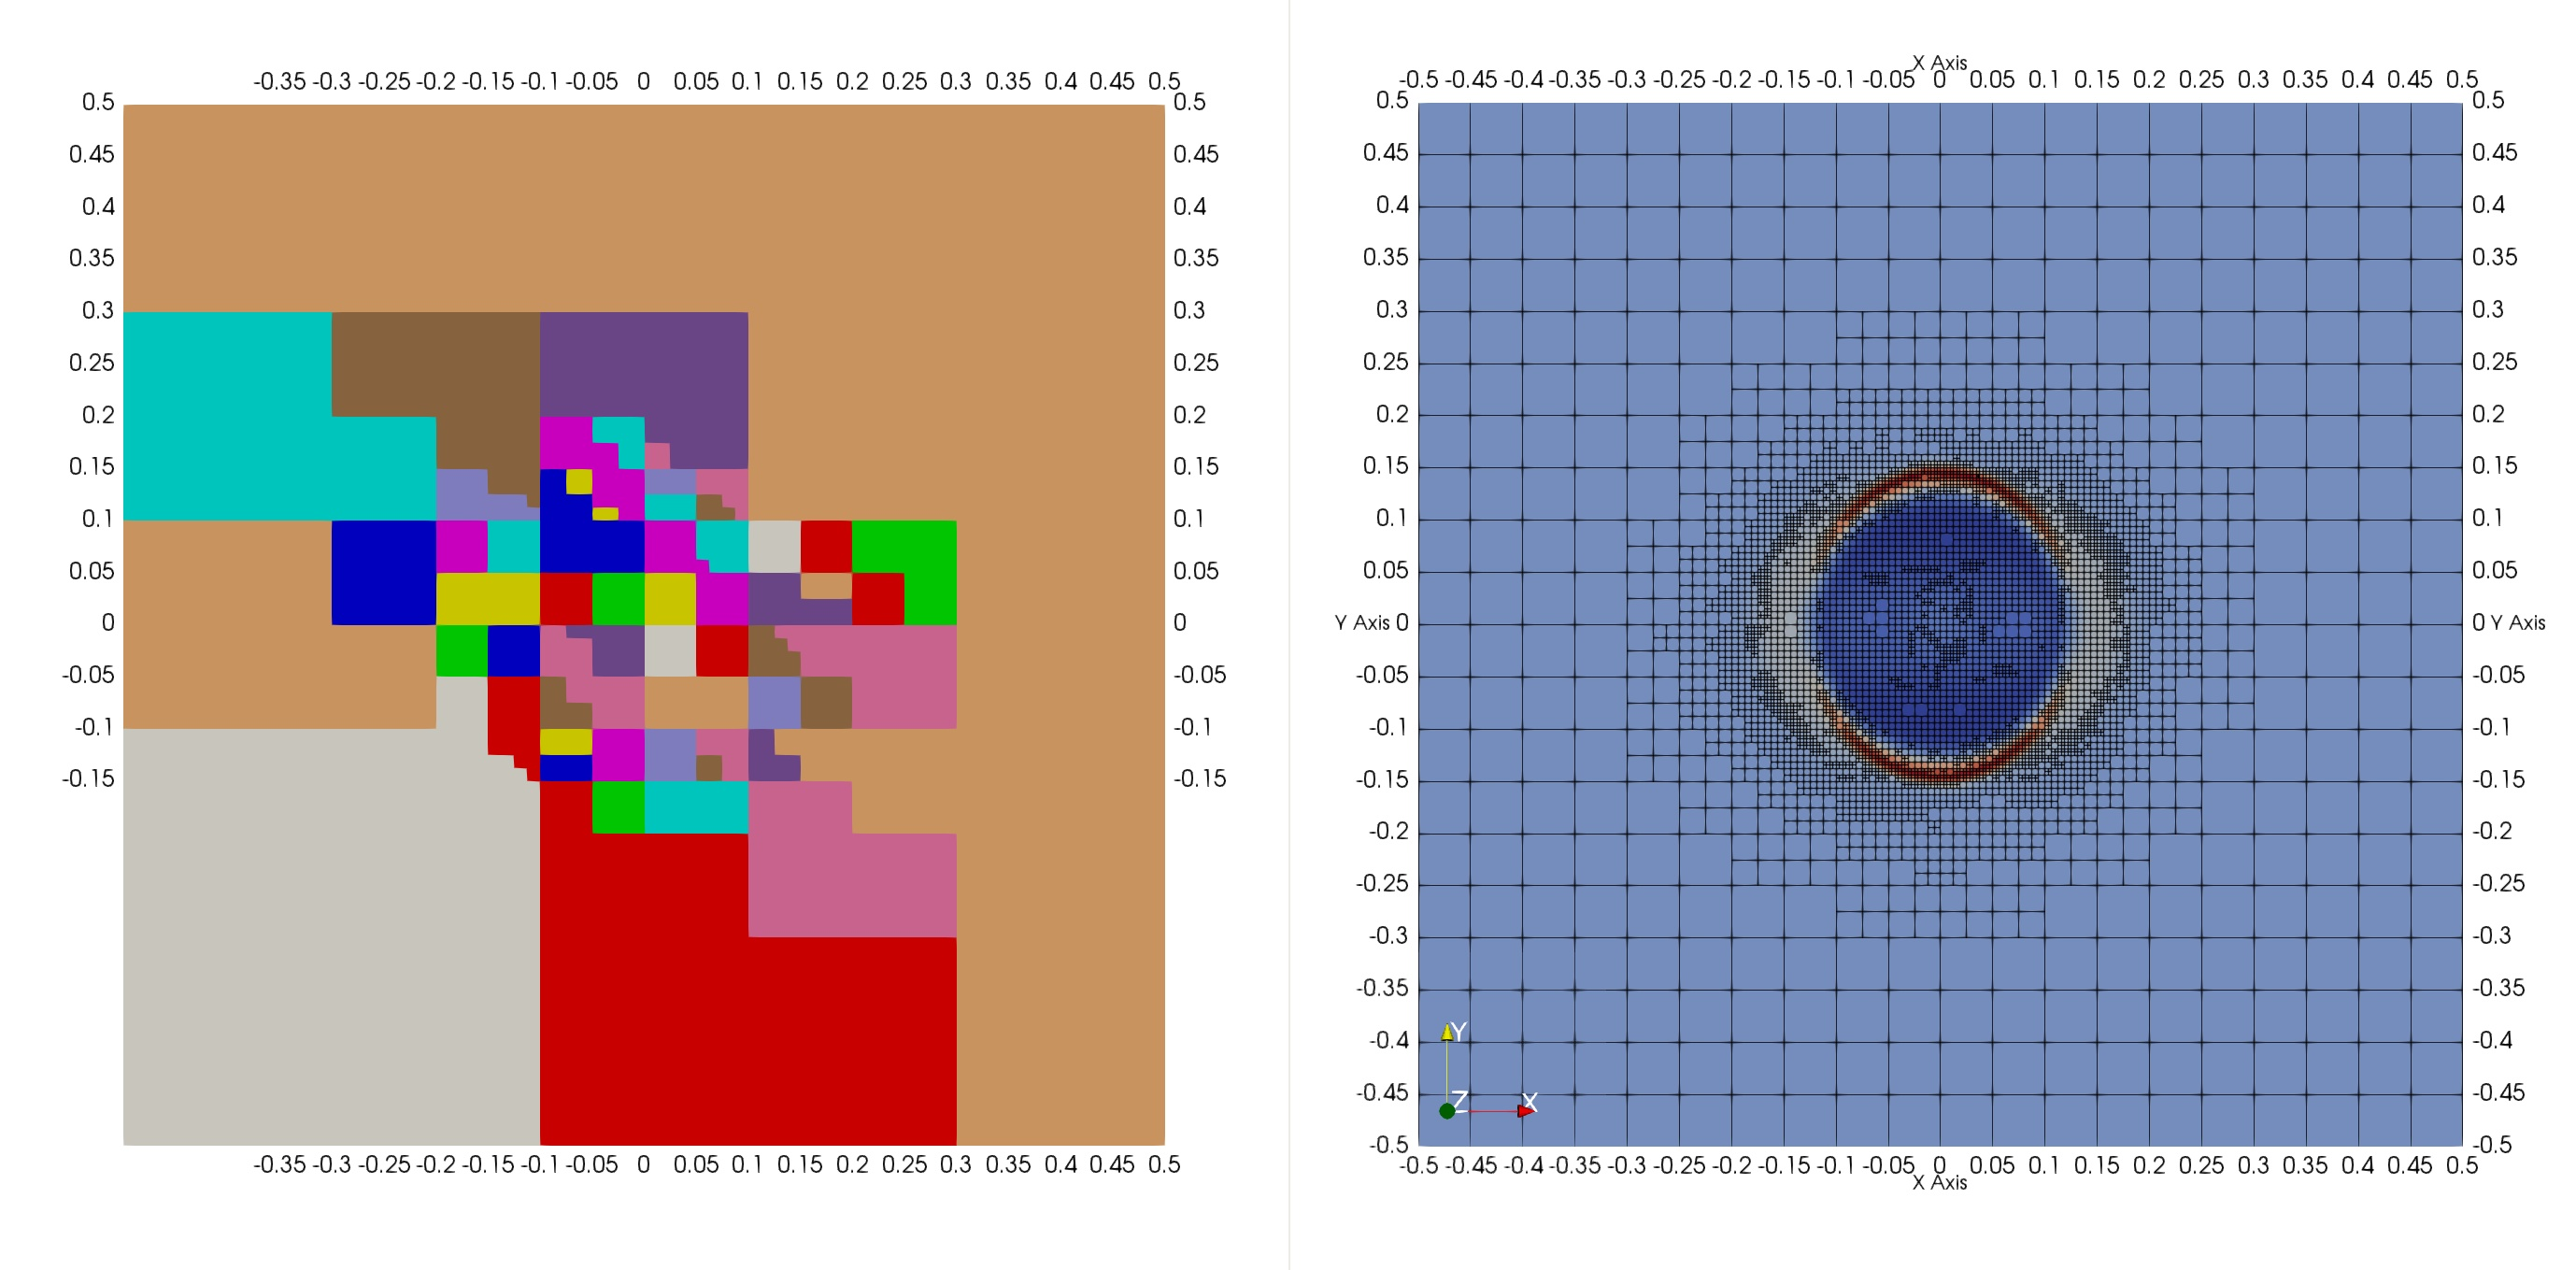
\includegraphics[width=0.87\textwidth]{img/mhd-blast/old/mya2.jpg}
	\caption{Obtained results, $t = 5\cdot 10^{-3}$, distribution of $\rho$ on elements in $T\lo\Omega\ro$ (right) and distribution of these elements to processors (left)}
	\label{figure:blastOldMyAdapt2}
	\end{center}
\end{figure}
\vspace{-8mm}

\begin{figure}[H]
	\begin{center}
		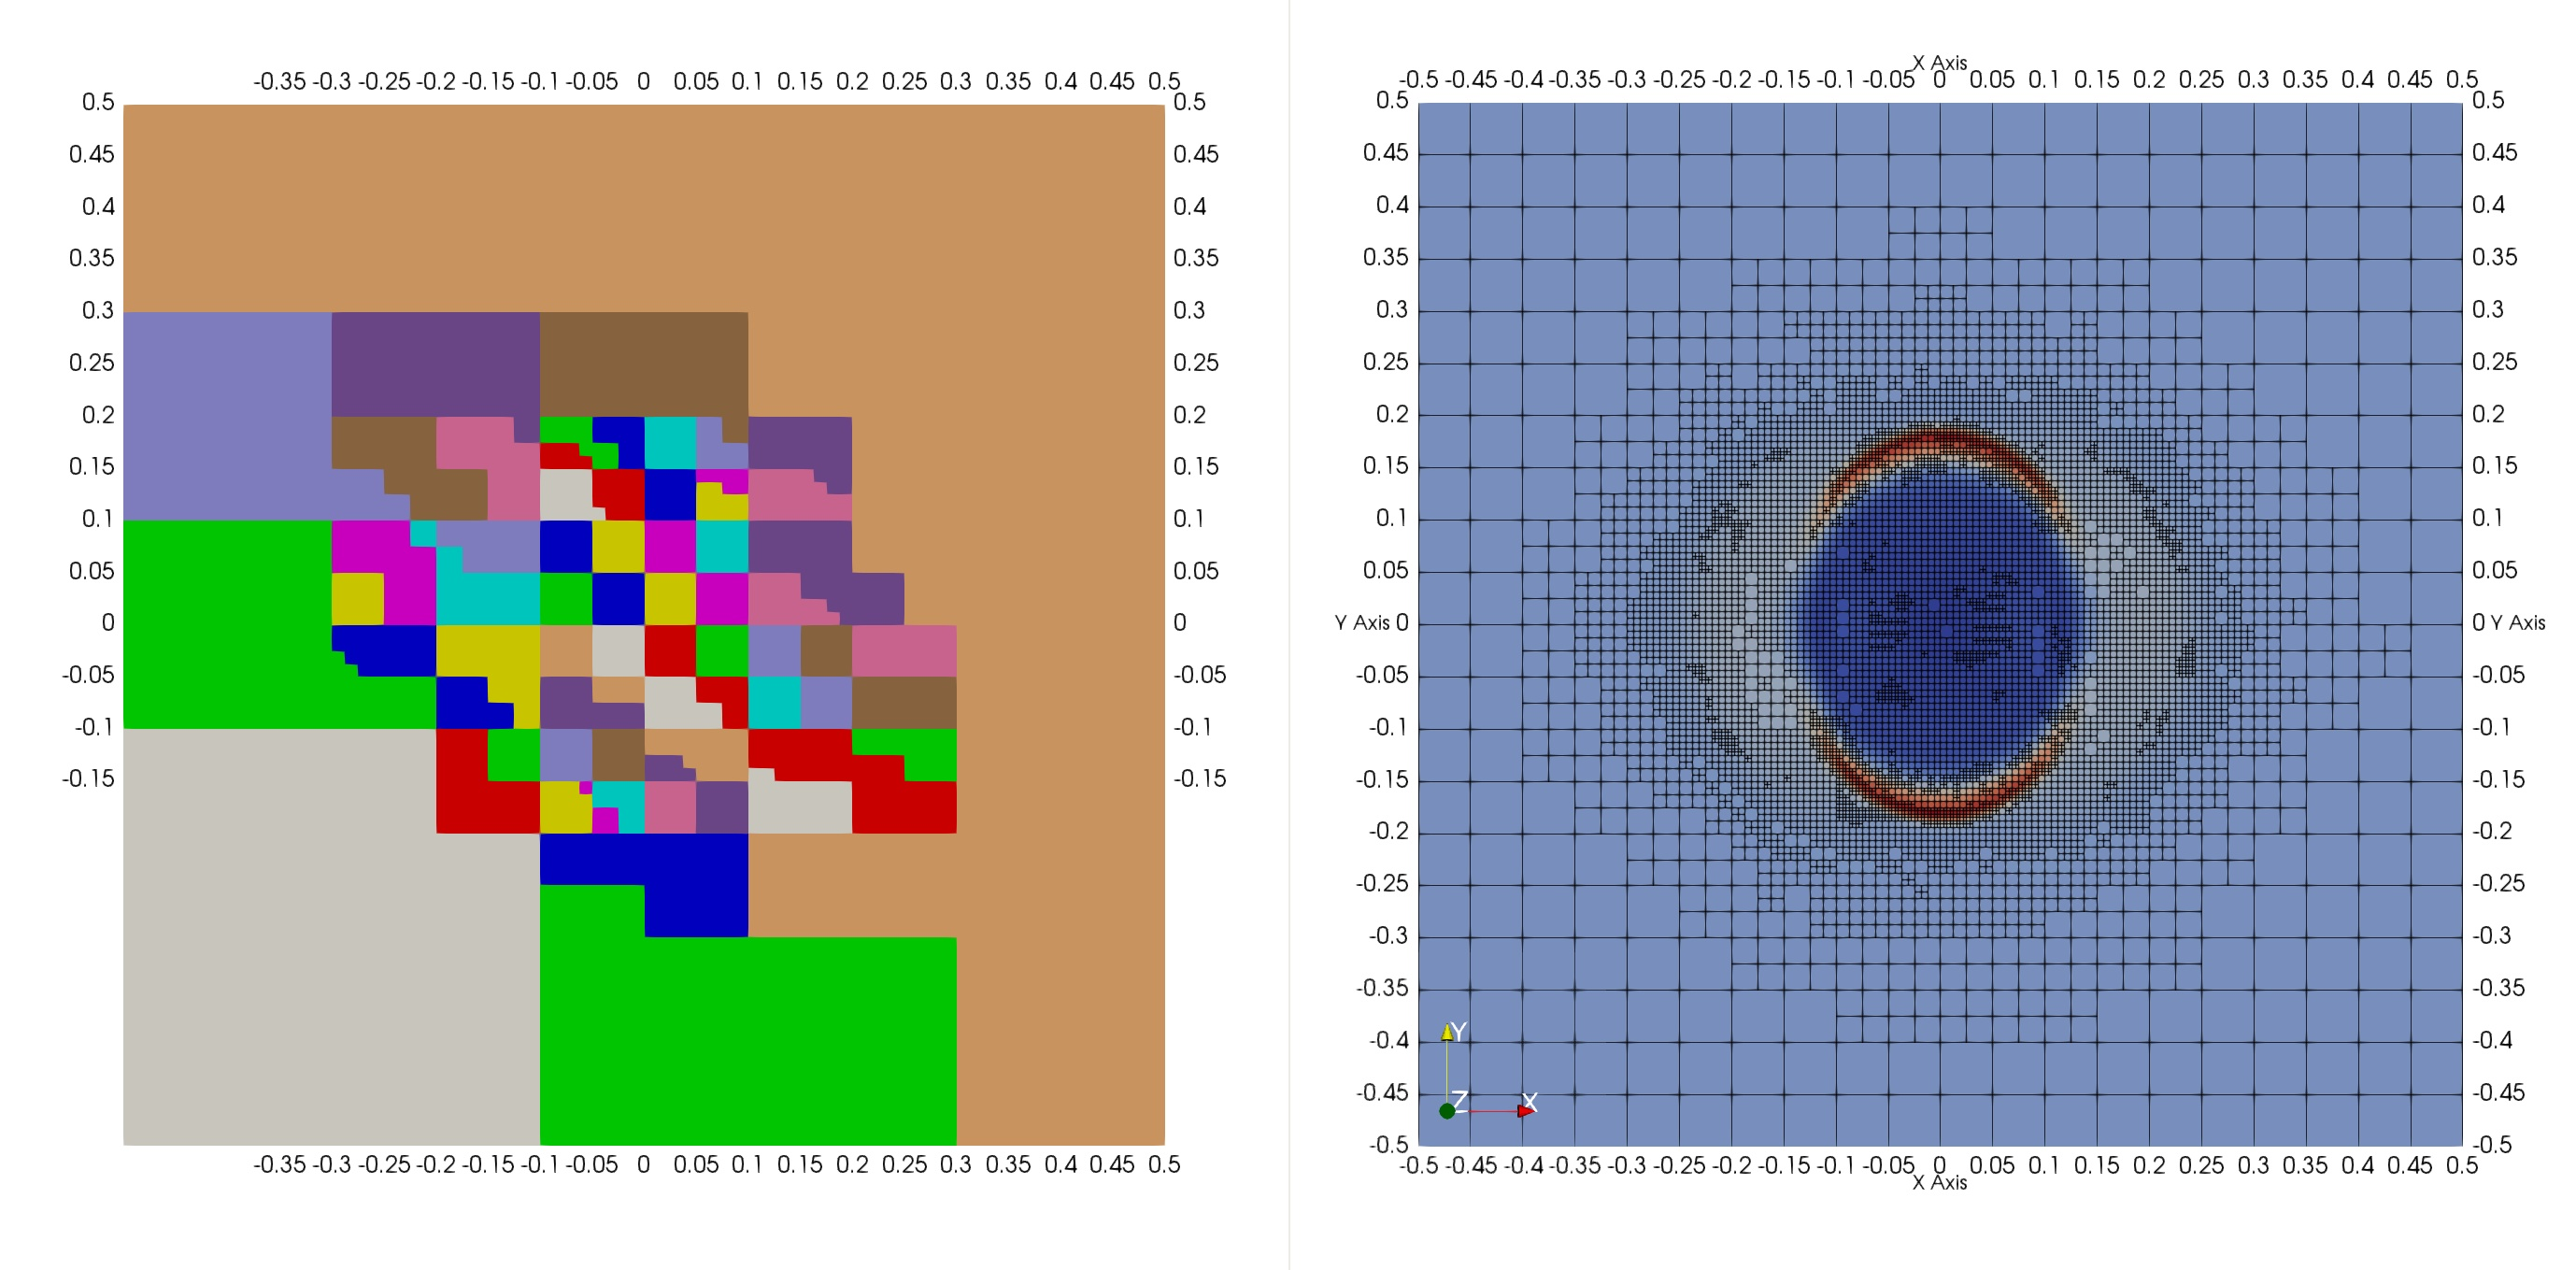
\includegraphics[width=0.87\textwidth]{img/mhd-blast/old/mya3.jpg}
	\caption{Obtained results, $t = 1\cdot 10^{-2}$, distribution of $\rho$ on elements in $T\lo\Omega\ro$ (right) and distribution of these elements to processors (left)}
	\label{figure:blastOldMyAdapt3}
	\end{center}
\end{figure}
\vspace{-8mm}

\begin{figure}[H]
	\begin{center}
		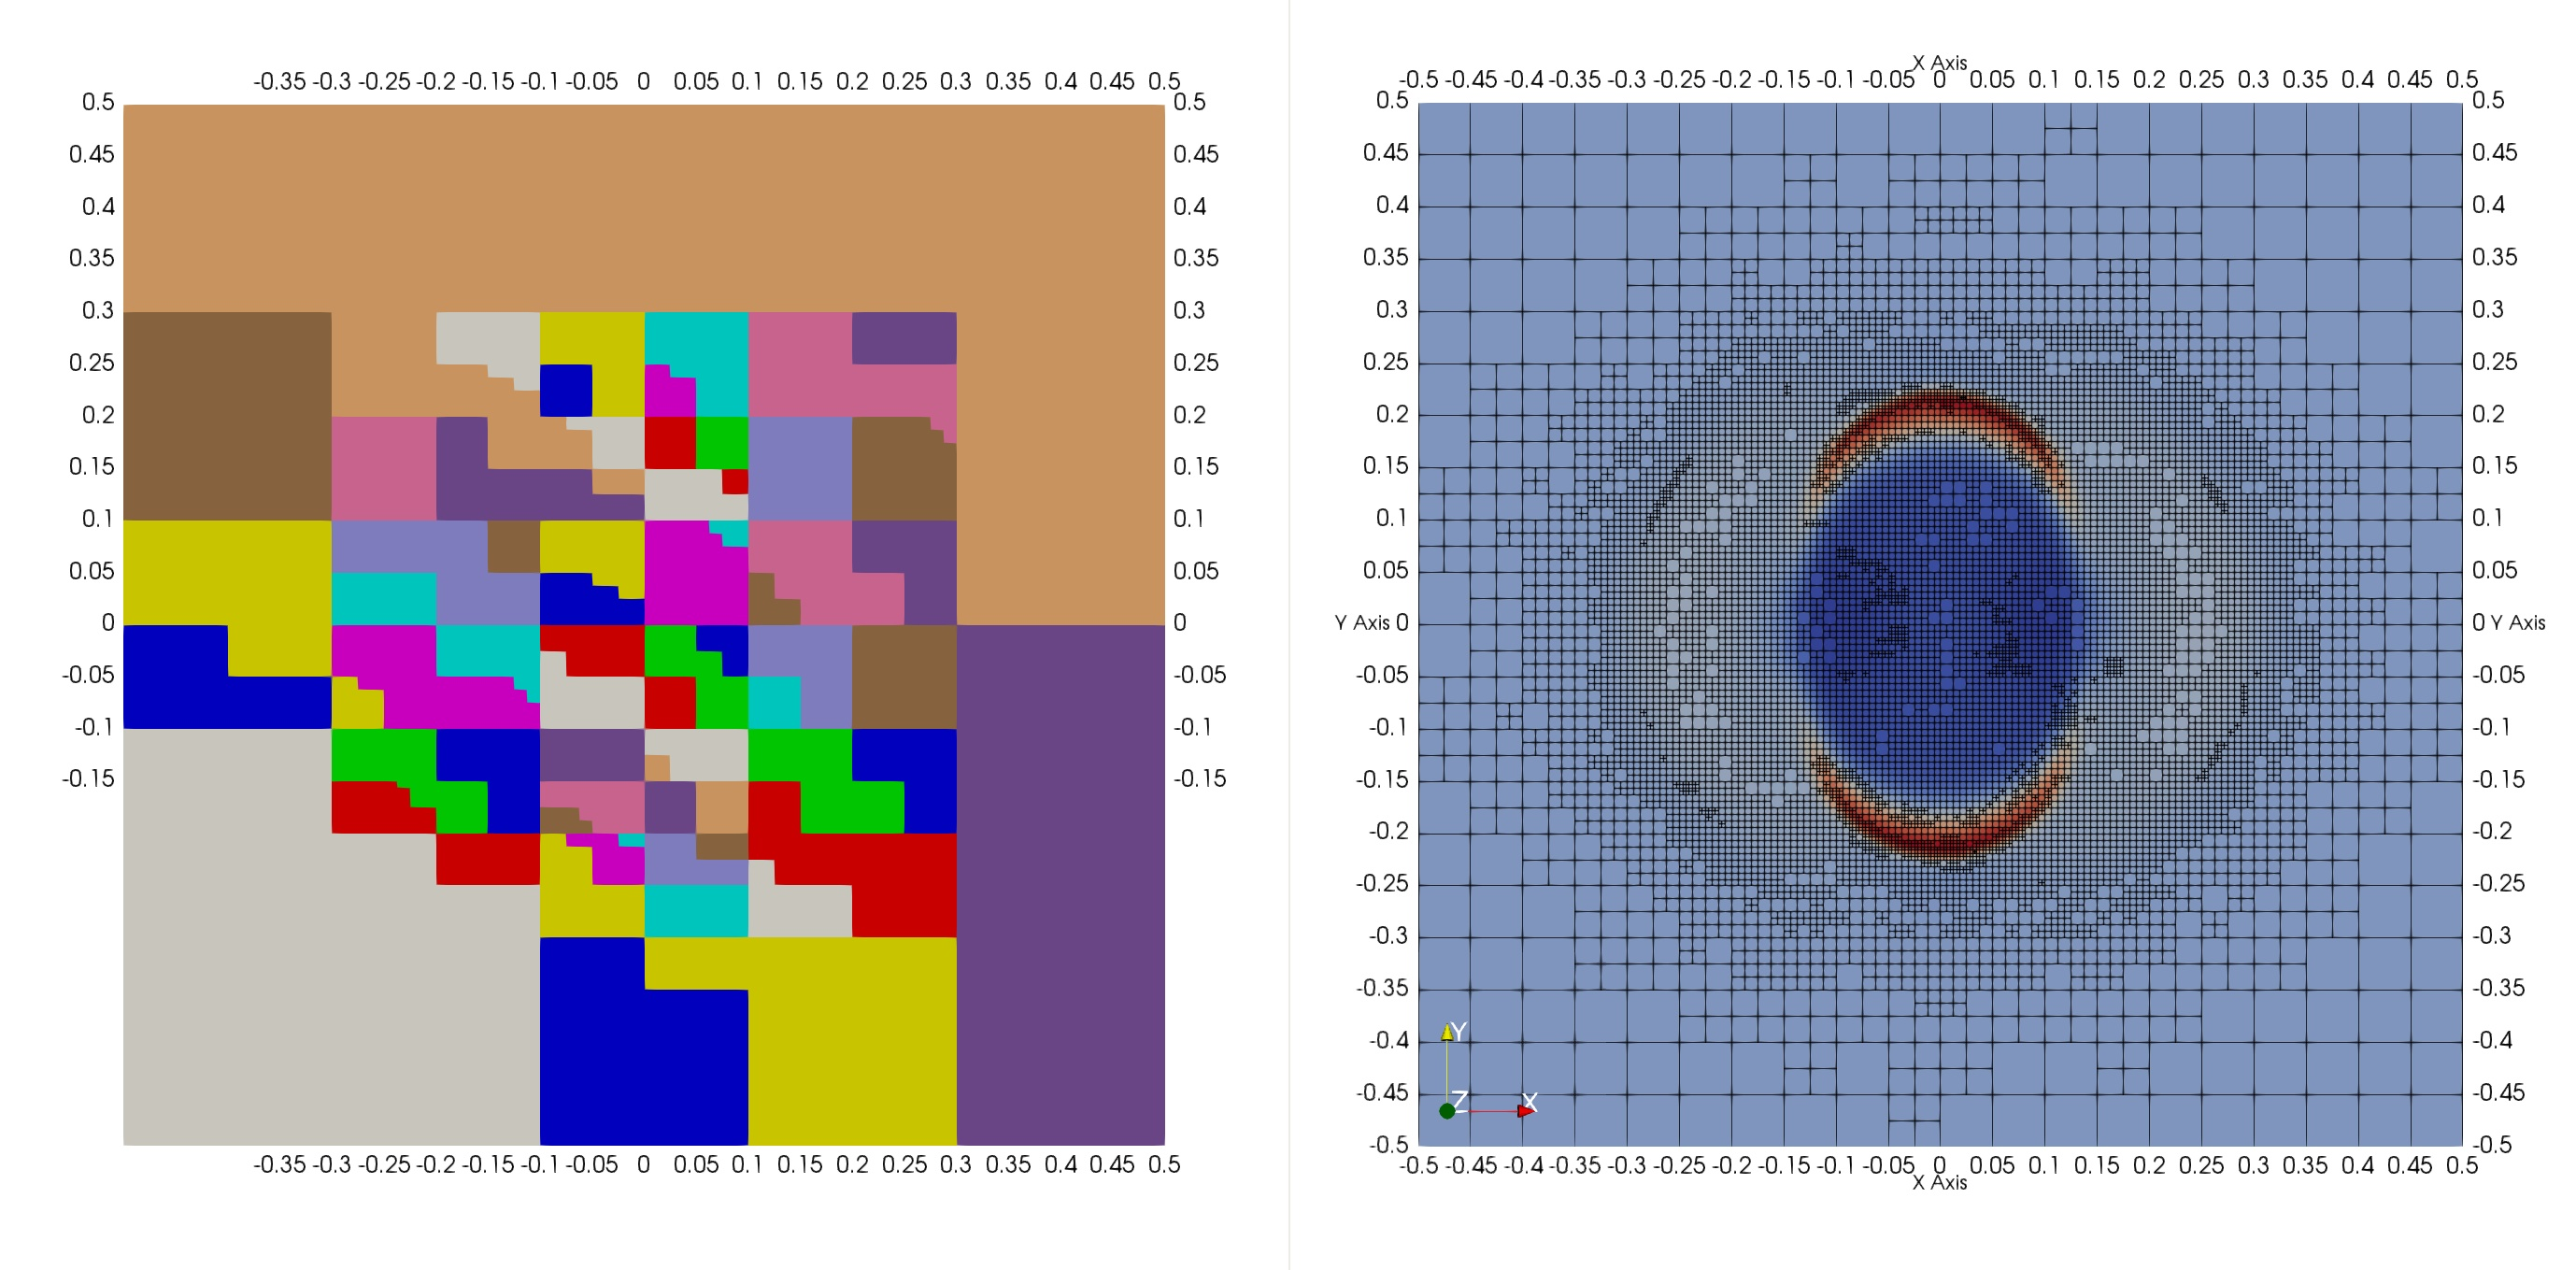
\includegraphics[width=0.87\textwidth]{img/mhd-blast/old/mya4.jpg}
	\caption{Obtained results, $t = 15\cdot 10^{-3}$, distribution of $\rho$ on elements in $T\lo\Omega\ro$ (right) and distribution of these elements to processors (left)}
	\label{figure:blastOldMyAdapt4}
	\end{center}
\end{figure}
\vspace{-8mm}

\begin{figure}[H]
	\begin{center}
		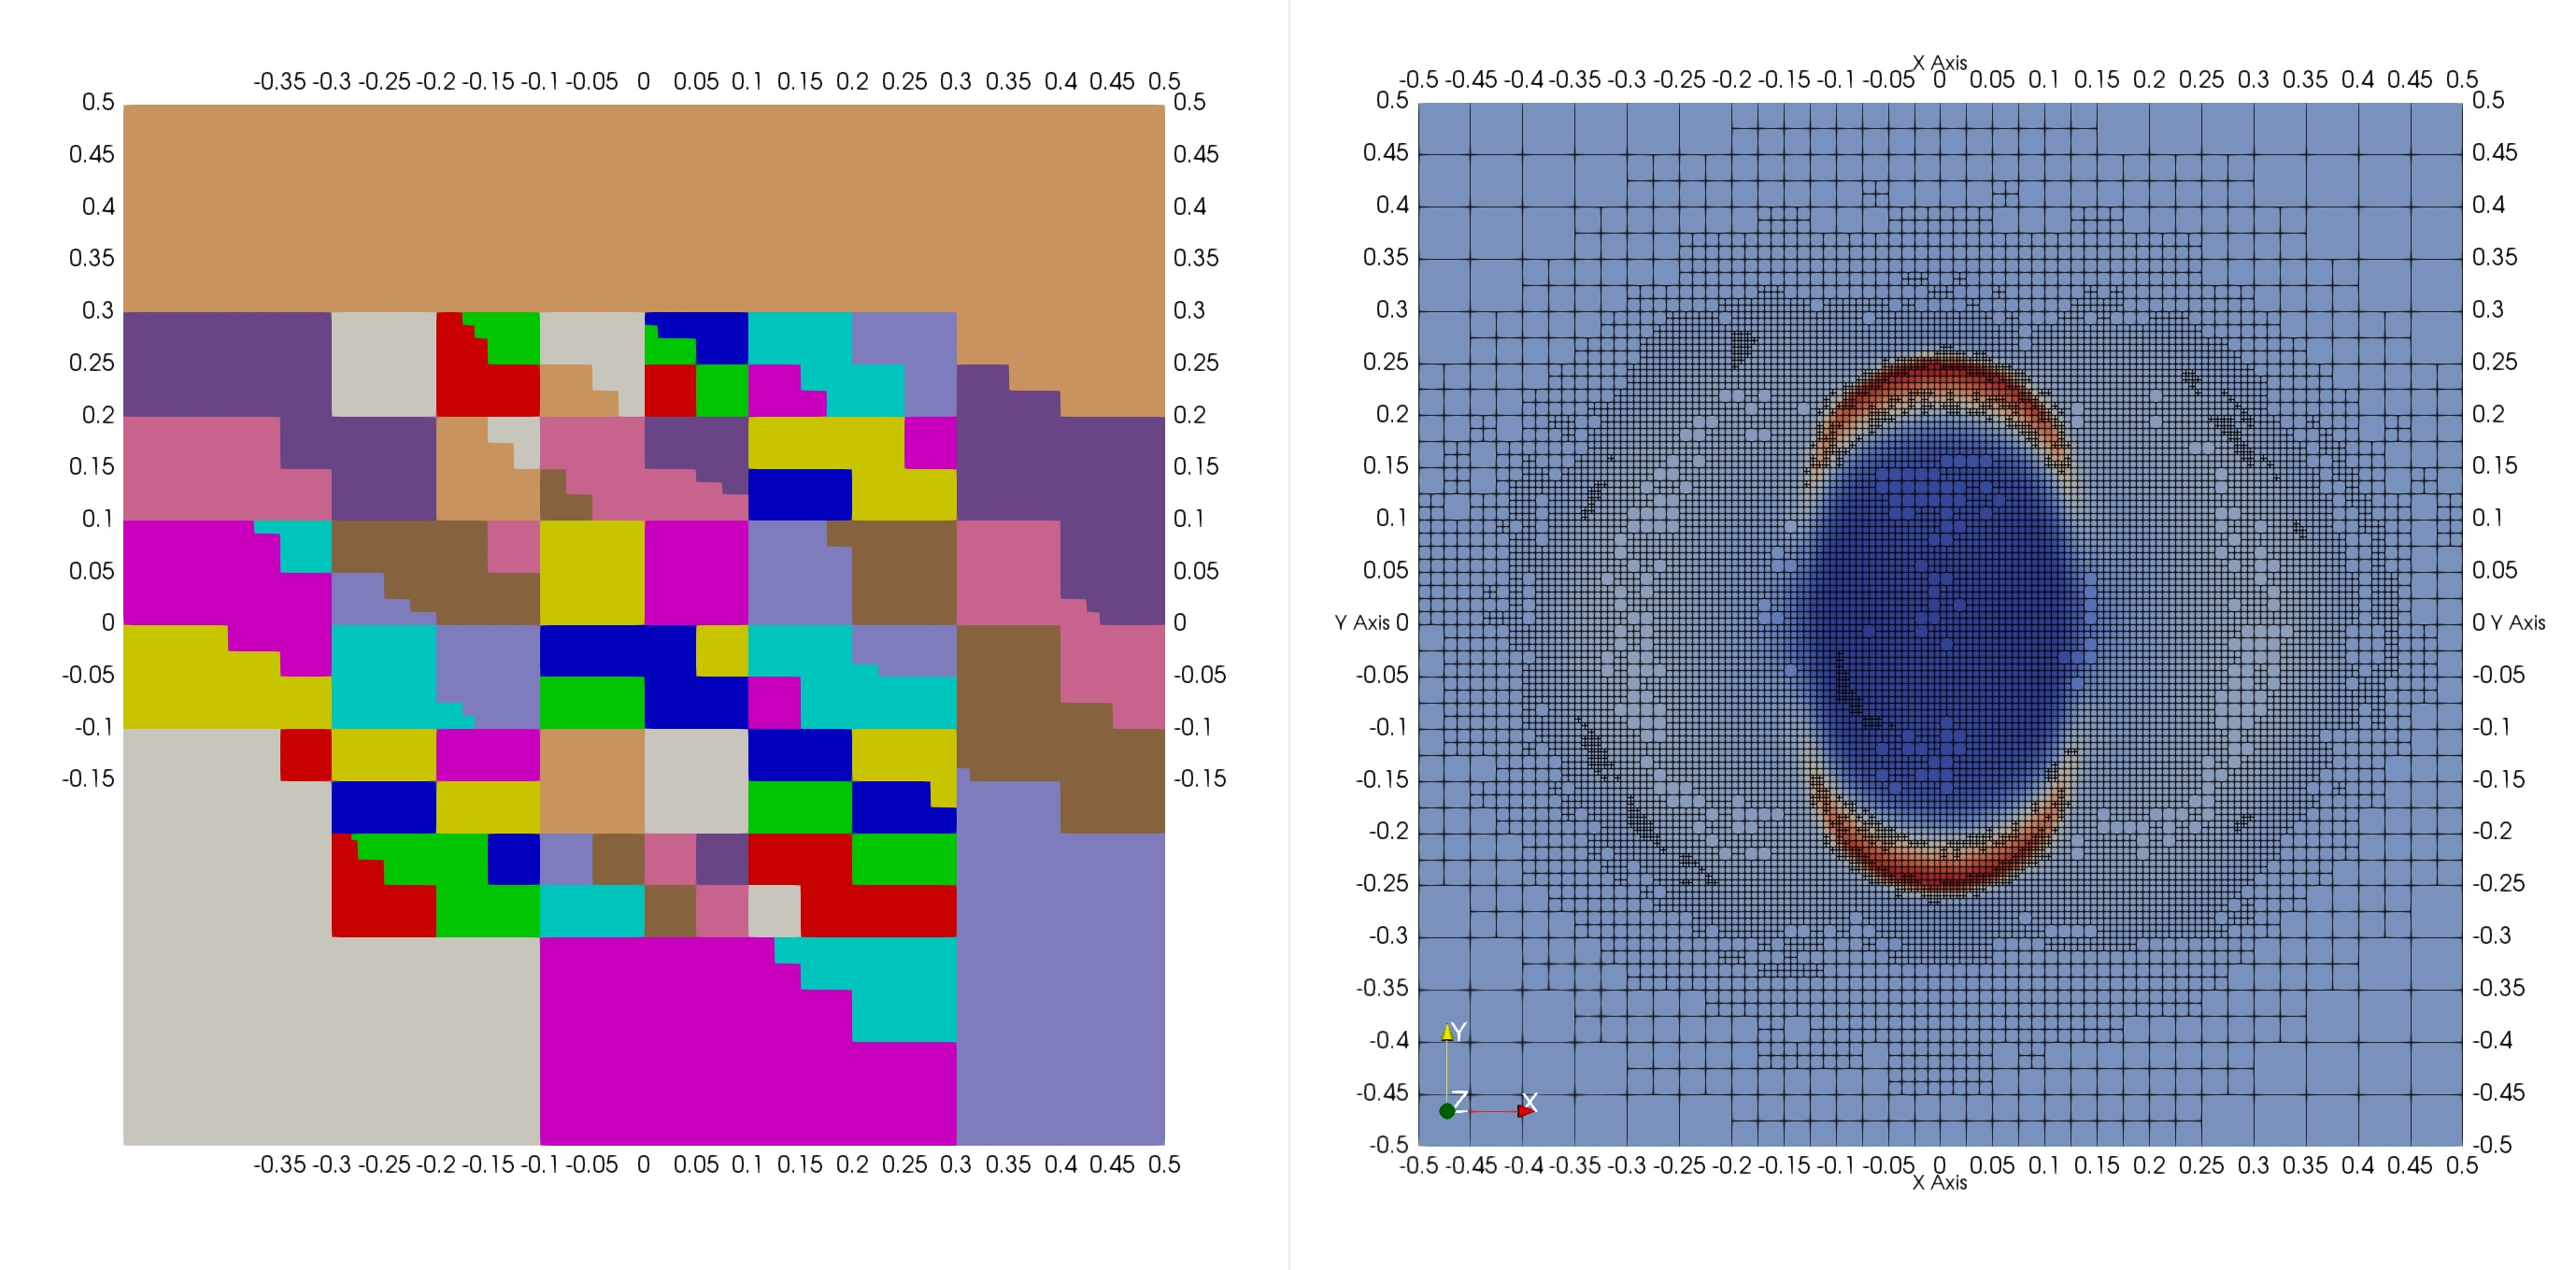
\includegraphics[width=0.87\textwidth]{img/mhd-blast/old/mya5.jpg}
	\caption{Obtained results, $t = 2\cdot 10^{-2}$, distribution of $\rho$ on elements in $T\lo\Omega\ro$ (right) and distribution of these elements to processors (left)}
	\label{figure:blastOldMyAdapt5}
	\end{center}
\end{figure}
\vspace{-8mm}

\begin{figure}[H]
	\begin{center}
		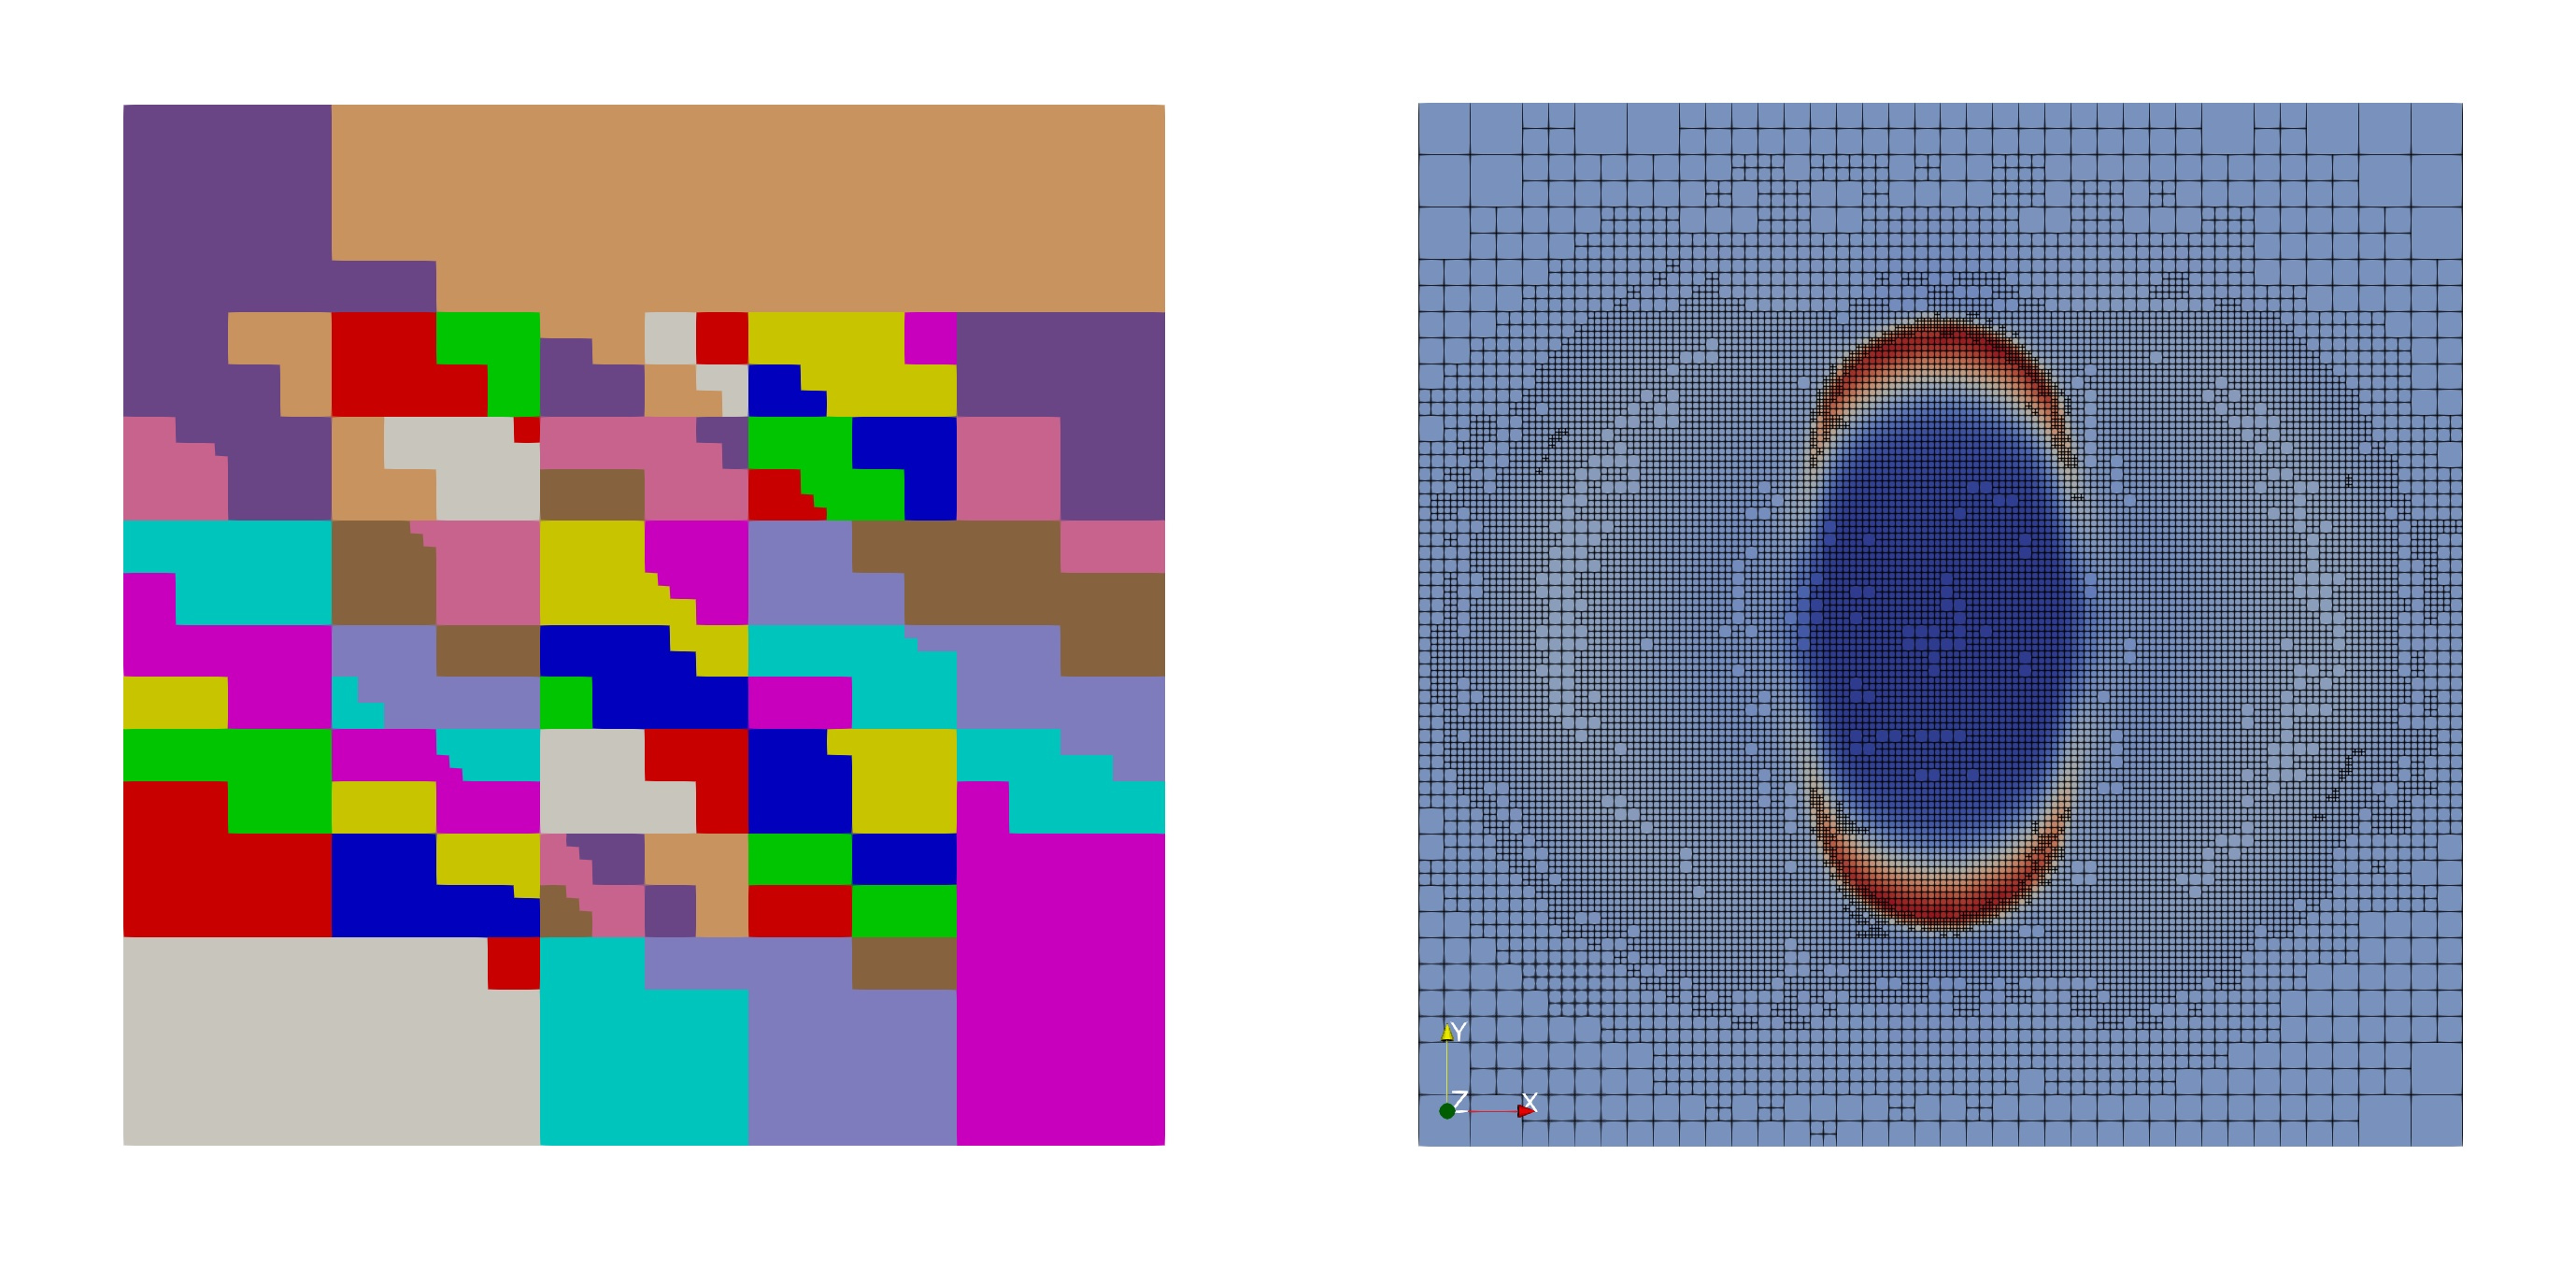
\includegraphics[width=0.87\textwidth]{img/mhd-blast/old/mya6.jpg}
	\caption{Obtained results, $t = 25\cdot 10^{-3}$, distribution of $\rho$ on elements in $T\lo\Omega\ro$ (right) and distribution of these elements to processors (left)}
	\label{figure:blastOldMyAdapt6}
	\end{center}
\end{figure}
\vspace{-8mm}

\subsubsection{MHD Blast - extended version}
\label{sec:blastNew}
An extended version of the benchmark has been used in \cite{blastNew1}, \cite{athenaBlast}, and a similar problem was used also in \cite{blastNew2} - the description of the benchmark is also available at:\url{http://www.astro.princeton.edu/~jstone/Athena/tests/blast/blast.html}.
In this version, the domain dimensions are set as a rectangle: $\Omega = [-0.5, 0.5] \times [-0.75, 0.75]$.
The initial conditions are a little different than in the case of \cref{mhdBlastOld}, and read:
\begin{align}
\label{mhdBlastNew}
\gamma & =  5 / 3\\ \nonumber
p_0\lo\bfx, t\ro & =  10\ \ \text{for}\ \left|\bfx\right| < 0.1\\ \nonumber
p_0\lo\bfx, t\ro & =  0.1\ \ \text{for}\ \left|\bfx\right| \geq 0.1\\ \nonumber
\rho\lo\bfx, t = 0\ro & =  1,\\ \nonumber
p\lo\bfx, t = 0\ro & =  p_0\lo\bfx, t\ro,\\ \nonumber
\bfu_1\lo\bfx, t = 0\ro & =  0,\\ \nonumber	
\bfu_2\lo\bfx, t = 0\ro & =  0,\\ \nonumber
\bfu_3\lo\bfx, t = 0\ro & =  0,\\ \nonumber
\bfB_1\lo\bfx, t = 0\ro & =  \frac{1}{\sqrt{2}},\\ \nonumber
\bfB_2\lo\bfx, t = 0\ro & =  \frac{1}{\sqrt{2}},\\ \nonumber
\bfB_3\lo\bfx, t = 0\ro & =  0,
\end{align}
with periodic boundary conditions on the top-bottom, and left-right parts of the boundary. That is, with respect to \cref{periodicMapping}, the two pairs $\Gamma_1, \Gamma_2, \Gamma_1^{'}, \Gamma_2^{'}$ are specified as follows:
\begin{align}
\Gamma_1 & = \left\{-0.5\right\} \times [-0.75, 0.75],\\
\Gamma_2 & = \left\{0.5\right\} \times [-0.75, 0.75],
\end{align}
and
\begin{align}
\Gamma_1^{'} & = [-0.5, 0.5] \times \left\{-0.75\right\},\\
\Gamma_2^{'} & = [-0.5, 0.5] \times \left\{0.75\right\}.
\end{align}

The solution image taken from \cite{blastNew1} is for comparison in \cref{figure:blastRef}.

\subsubsection{Results}
The first set of results are from calculations using piecewise-constant elements, on three successively uniformly refined meshes. The meshes used for computations \crefrange{figure:blastNew01}{figure:blastNew06} contained:
\begin{itemize}
\item $100 \times 150$ elements (left)
\item $200 \times 300$ elements (middle)
\item $400 \times 600$ elements (right)
\end{itemize}

\begin{figure}[H]
	\begin{center}
		\includegraphics[width=0.98\textwidth]{img/mhd-blast/new/blast,noadapt1.jpg}
\vspace{-3mm}
	\caption{Obtained results, $t \approx 0.1$, distribution of $\rho$ (top), with line distribution along bottom-left $\rightarrow$ top-right diagonal (bottom)}
	\label{figure:blastNew01}
	\end{center}
\end{figure}
\vspace{-10mm}

\begin{figure}[H]
	\begin{center}
		\includegraphics[width=0.98\textwidth]{img/mhd-blast/new/blast,noadapt3.jpg}
\vspace{-3mm}
	\caption{Obtained results, $t = \approx 0.2$, distribution of $\rho$ (top), with line distribution along bottom-left $\rightarrow$ top-right diagonal (bottom)}
	\label{figure:blastNew02}
	\end{center}
\end{figure}
\vspace{-10mm}

\begin{figure}[H]
	\begin{center}
		\includegraphics[width=0.98\textwidth]{img/mhd-blast/new/blast,noadapt5.jpg}
\vspace{-3mm}
	\caption{Obtained results, $t \approx 0.3$, distribution of $\rho$ (top), with line distribution along bottom-left $\rightarrow$ top-right diagonal (bottom)}
	\label{figure:blastNew03}
	\end{center}
\end{figure}
\vspace{-10mm}

\begin{figure}[H]
	\begin{center}
		\includegraphics[width=0.98\textwidth]{img/mhd-blast/new/blast,noadapt9.jpg}
\vspace{-3mm}
	\caption{Obtained results, $t \approx 0.45$, distribution of $\rho$ (top), with line distribution along bottom-left $\rightarrow$ top-right diagonal (bottom)}
	\label{figure:blastNew04}
	\end{center}
\end{figure}
\vspace{-10mm}

\begin{figure}[H]
	\begin{center}
		\includegraphics[width=0.98\textwidth]{img/mhd-blast/new/blast,noadapt14.jpg}
\vspace{-3mm}
	\caption{Obtained results, $t = \approx 0.75$, distribution of $\rho$ (top), with line distribution along bottom-left $\rightarrow$ top-right diagonal (bottom)}
	\label{figure:blastNew05}
	\end{center}
\end{figure}
\vspace{-10mm}

\begin{figure}[H]
	\begin{center}
		\includegraphics[width=0.98\textwidth]{img/mhd-blast/new/blast,noadapt18.jpg}
\vspace{-3mm}
	\caption{Obtained results, $t \approx 0.95$, distribution of $\rho$ (top), with line distribution along bottom-left $\rightarrow$ top-right diagonal (bottom)}
	\label{figure:blastNew06}
	\end{center}
\end{figure}
\vspace{-8mm}

It is clearly visible, that the solution is somehow smeared, and the uniform mesh refinements improve the situation, but not greatly, and for a large cost of storage size for storing much more mesh elements.
\paragraph{}
In order to amend the situation, and be able to obtain a higher-quality solution with a reasonable number of mesh elements, piecewise-linear basis functions need to be used. Results with piecewise-linear basis functions, on three successively uniformly refined meshes are given in \crefrange{figure:blastNew11}{figure:blastNew16}. The meshes for these computations contained:
\begin{itemize}
\item $50 \times 75$ elements (left)
\item $100 \times 150$ elements (middle)
\item $200 \times 300$ elements (right)
\end{itemize}

\begin{figure}[H]
	\begin{center}
		\includegraphics[width=0.92\textwidth]{img/mhd-blast/new/blast,1noadapt1.jpg}
\vspace{-3mm}
	\caption{Obtained results, $t \approx 0.1$, distribution of $\rho$ (top), with line distribution along bottom-left $\rightarrow$ top-right diagonal (bottom)}
	\label{figure:blastNew11}
	\end{center}
\end{figure}
\vspace{-10mm}

\begin{figure}[H]
	\begin{center}
		\includegraphics[width=0.92\textwidth]{img/mhd-blast/new/blast,1noadapt3.jpg}
\vspace{-3mm}
	\caption{Obtained results, $t = \approx 0.2$, distribution of $\rho$ (top), with line distribution along bottom-left $\rightarrow$ top-right diagonal (bottom)}
	\label{figure:blastNew12}
	\end{center}
\end{figure}
\vspace{-10mm}

\begin{figure}[H]
	\begin{center}
		\includegraphics[width=0.92\textwidth]{img/mhd-blast/new/blast,1noadapt5.jpg}
\vspace{-3mm}
	\caption{Obtained results, $t \approx 0.3$, distribution of $\rho$ (top), with line distribution along bottom-left $\rightarrow$ top-right diagonal (bottom)}
	\label{figure:blastNew13}
	\end{center}
\end{figure}
\vspace{-10mm}

\begin{figure}[H]
	\begin{center}
		\includegraphics[width=0.92\textwidth]{img/mhd-blast/new/blast,1noadapt9.jpg}
\vspace{-3mm}
	\caption{Obtained results, $t \approx 0.45$, distribution of $\rho$ (top), with line distribution along bottom-left $\rightarrow$ top-right diagonal (bottom)}
	\label{figure:blastNew14}
	\end{center}
\end{figure}
\vspace{-10mm}

\begin{figure}[H]
	\begin{center}
		\includegraphics[width=0.92\textwidth]{img/mhd-blast/new/blast,1noadapt14.jpg}
\vspace{-3mm}
	\caption{Obtained results, $t = \approx 0.75$, distribution of $\rho$ (top), with line distribution along bottom-left $\rightarrow$ top-right diagonal (bottom)}
	\label{figure:blastNew15}
	\end{center}
\end{figure}
\vspace{-10mm}

\begin{figure}[H]
	\begin{center}
		\includegraphics[width=0.92\textwidth]{img/mhd-blast/new/blast,1noadapt18.jpg}
\vspace{-3mm}
	\caption{Obtained results, $t \approx 0.95$, distribution of $\rho$ (top), with line distribution along bottom-left $\rightarrow$ top-right diagonal (bottom)}
	\label{figure:blastNew16}
	\end{center}
\end{figure}
\vspace{-6mm}

Now, the solution with piecewise-linear functions is of much higher quality and the solution snapshots displayed in \cref{figure:blastFinal} are practically identical (and even more detailed) as the solution from \cite{blastNew1} in \cref{figure:blastRef}. Of course, this comes at a price of increased number of degrees of freedom, and associated increase in the storage size requirements, as well as the computation time, with respect to the solution with piecewise-constant basis functions.

\begin{figure}[H]
	\begin{center}
		\includegraphics[width=0.8\textwidth]{img/mhd-blast/new/ref.jpg}
	\caption{Reference solution, $\rho$ distribution, $t \approx 0.2$ (left), $t \approx 1.0$ (right), from \cite{blastNew1}}
	\label{figure:blastRef}
	\end{center}
\end{figure}
\vspace{-6mm}
\begin{figure}[H]
	\begin{center}
		\includegraphics[width=0.8\textwidth]{img/mhd-blast/new/ref-result.jpg}
	\caption{Obtained $\rho$ distribution, $t \approx 0.2$ (left), $t \approx 1.0$ (right)}
	\label{figure:blastFinal}
	\end{center}
\end{figure}
\vspace{-4mm}

\subsubsection{AMR for MHD Blast - extended version}
One can see, that for the finest mesh of $200\times300$ elements, the solution obtained shows very detailed features, and is arguably of even higher quality than the reference one from \cite{blastNew1}. However, the calculation needs
\be
200 \times 300\ = 60000\ \text{elements},
\ee
where each element contains $4$ basis functions for each of $\rho, p, \pi_1, \pi_2, \pi_3$, and $11$ basis functions for $\bfB$, that is $31$ basis functions per element, in total $60000 \times 31 = 1860000$ degrees of freedom (DOFs). This number can be decreased, while keeping the same (or even higher) solution quality, with AMR - as illustrated in \crefrange{figure:amrBlast1}{figure:amrBlast8} below. On each of \crefrange{figure:amrBlast1}{figure:amrBlast8}, the solution is displayed on the left, the adapted mesh in the middle, and the owning processor of a chunk of elements on the right. Note that there were $96$ processors used for the computation.

\begin{figure}[H]
	\begin{center}
		\includegraphics[width=0.95\textwidth]{img/mhd-blast/new/adapt-full0.jpg}
\vspace{-3mm}
	\caption{Obtained $\rho$ distribution, mesh elements, and their owning processor. Time $t\approx 0.05$.}
	\label{figure:amrBlast1}
	\end{center}
\end{figure}
\vspace{-10mm}

\begin{figure}[H]
	\begin{center}
		\includegraphics[width=0.95\textwidth]{img/mhd-blast/new/adapt-full1.jpg}
\vspace{-3mm}
	\caption{Obtained $\rho$ distribution, mesh elements, and their owning processor. Time $t\approx 0.1$.}
	\label{figure:amrBlast2}
	\end{center}
\end{figure}
\vspace{-10mm}

\begin{figure}[H]
	\begin{center}
		\includegraphics[width=0.95\textwidth]{img/mhd-blast/new/adapt-full2.jpg}
\vspace{-3mm}
	\caption{Obtained $\rho$ distribution, mesh elements, and their owning processor. Time $t\approx 0.15$.}
	\label{figure:amrBlast3}
	\end{center}
\end{figure}
\vspace{-10mm}

\begin{figure}[H]
	\begin{center}
		\includegraphics[width=0.95\textwidth]{img/mhd-blast/new/adapt-full3.jpg}
\vspace{-3mm}
	\caption{Obtained $\rho$ distribution, mesh elements, and their owning processor. Time $t\approx 0.2$.}
	\label{figure:amrBlast4}
	\end{center}
\end{figure}
\vspace{-10mm}

\begin{figure}[H]
	\begin{center}
		\includegraphics[width=0.95\textwidth]{img/mhd-blast/new/adapt-full6.jpg}
\vspace{-3mm}
	\caption{Obtained $\rho$ distribution, mesh elements, and their owning processor. Time $t\approx 0.35$.}
	\label{figure:amrBlast5}
	\end{center}
\end{figure}
\vspace{-10mm}

\begin{figure}[H]
	\begin{center}
		\includegraphics[width=0.95\textwidth]{img/mhd-blast/new/adapt-full10.jpg}
\vspace{-3mm}
	\caption{Obtained $\rho$ distribution, mesh elements, and their owning processor. Time $t\approx 0.55$.}
	\label{figure:amrBlast6}
	\end{center}
\end{figure}
\vspace{-10mm}


\begin{figure}[H]
	\begin{center}
		\includegraphics[width=0.95\textwidth]{img/mhd-blast/new/adapt-full13.jpg}
\vspace{-3mm}
	\caption{Obtained $\rho$ distribution, mesh elements, and their owning processor. Time $t\approx 0.7$.}
	\label{figure:amrBlast7}
	\end{center}
\end{figure}
\vspace{-10mm}


\begin{figure}[H]
	\begin{center}
		\includegraphics[width=0.95\textwidth]{img/mhd-blast/new/adapt-full16.jpg}
\vspace{-3mm}
	\caption{Obtained $\rho$ distribution, mesh elements, and their owning processor. Time $t\approx 0.85$.}
	\label{figure:amrBlast8}
	\end{center}
\end{figure}
\vspace{-6mm}
In the \cref{table:meshElems}, mesh elements counts for all the displayed snapshots are given. Note that, as described in \cref{algorithm:AMRFull}, the number of elements constantly evolves.

\begin{table}[H]
    \begin{tabular}
		{ | l | l | p{5cm} |}
		\hline
    \textbf{Time step} & \textbf{Number of mesh elements} & \textbf{Number of DOFs} \\
		\hline
    $t\approx 0.05$ & 5880 & 182280  \\ \hline
    $t\approx 0.1$ & 7332 & 227292  \\ \hline
    $t\approx 0.15$ & 8649 & 268119  \\ \hline
    $t\approx 0.2$ & 10044 & 311364  \\ \hline
    $t\approx 0.35$ & 14013 & 434403  \\ \hline
    $t\approx 0.55$ & 16578  & 513918 \\ \hline
    $t\approx 0.7$ & 17192 & 532952  \\ \hline
    $t\approx 0.85$ & 18708 & 579948  \\ \hline
    \end{tabular}
	\caption{Mesh elements and DOFs counts for snapshots displayed in \crefrange{figure:amrBlast1}{figure:amrBlast8}}
\label{table:meshElems}
\end{table}

From \cref{table:meshElems}, it is cleary visible, that even for such a complex, and seemingly chaotic example, the AMR approach can cut down the number of mesh elements / DOFs radically, by 70-90 \%, while achieving comparable results. 

\subsection{Orszag-Tang vortex}
This problem was first described in \cite{vortex} and has been extensively used as a benchmark for 2- and 3- dimensional MHD code (\cite{blast0}, \cite{blast1}, \cite{honzaFem}, \cite{otnew}, and many others). It is a simple model of the evolution of MHD turbulence including interactions between the several shock waves that appear. The Orszag-Tang system is defined by the initial conditions:
\begin{align}
\rho_0 & =  \frac{25}{36 \pi}\\ \nonumber
p_0 & =  \frac{5}{12 \pi}\\  \nonumber
B_0 & =  \sqrt{\frac{1}{4 \pi}}\\ \nonumber
\gamma & =  5 / 3\\ \nonumber
\rho\lo\bfx, t = 0\ro & =  \rho_0,\\ \nonumber
p\lo\bfx, t = 0\ro & =  p_0,\\ \nonumber
\bfu_1\lo\bfx, t = 0\ro & =  -\sin(2 \pi y),\\ \nonumber
\bfu_2\lo\bfx, t = 0\ro & =  \sin(2 \pi x),\\ \nonumber
\bfu_3\lo\bfx, t = 0\ro & =  0,\\ \nonumber
\bfB_1\lo\bfx, t = 0\ro & =  -B_0 \sin(2 \pi y),\\ \nonumber
\bfB_2\lo\bfx, t = 0\ro & =  B_0 \sin(4 \pi x),\\ \nonumber
\bfB_3\lo\bfx, t = 0\ro & =  0,\\ \nonumber
U\lo\bfx, t = 0\ro & =  \frac{p_0}{\gamma - 1} + U_m\lo\bfx, t\ro + U_k\lo\bfx, t\ro,
\end{align}
where the last term is an application of \cref{magU,kinU,presU}. The domain $\Omega$ is set as $\Omega = [0, 1] \times [0, 1]$ and the problem is equipped with periodic boundary conditions on the top-bottom, and left-right parts of the boundary, similarly as in \cref{sec:blastNew}. This configuration is strongly unstable, leading to a wide spectrum of propagating MHD modes and shock waves.
\paragraph{}
As before, in order to compare with reference papers, figures are presented from these papers - see \cref{figure:otRef}. The images are taken from pages 30 (\cite{blast1}), and 20/282 (\cite{blast0}) respectively. All are taken at $t = 0.5$.

\begin{figure}[H]
\centering
\begin{subfigure}[b]{0.4\textwidth}\vspace{12mm}\includegraphics[width=\textwidth]{img/ot/ref-londrillo-pressure.jpg}\end{subfigure}
\begin{subfigure}[b]{0.4\textwidth}\includegraphics[width=\textwidth]{img/ot/ref-zachary-pressure-contour.jpg}\end{subfigure}
\\
\begin{subfigure}[b]{0.75\textwidth}\includegraphics[width=\textwidth]{img/ot/ref-zachary-pressure-profile.jpg}\end{subfigure}
\caption{$p$ isolines from \cite{blast1} (top left), $p$ isolines from \cite{blast0} (top right), $p$ along $y = 0.3125$ from \cite{blast0} (bottom).}
\label{figure:otRef}
\end{figure}

Results obtained in the implemented software are presented in \crefrange{figure:myOt1}{figure:myOt7}. The result on \cref{figure:myOt7} is obviously in almost exact accordance with \cref{figure:otRef}. Also, similar number of elements was used - $200$ in the computation in the implemented software, and $192$ in the reference computation.

\begin{figure}[H]
	\centering
	\includegraphics[width=0.92\textwidth]{img/ot/my1new.jpg}
\vspace{-2mm}
\caption{$p$ distribution in $\Omega$ and $p$ along $y = 0.3125$, $t = 0.03$}
\label{figure:myOt1}
\end{figure}
\vspace{-4mm}

\begin{figure}[H]
	\centering
	\includegraphics[width=0.92\textwidth]{img/ot/my2new.jpg}
\vspace{-2mm}
\caption{$p$ distribution in $\Omega$ and $p$ along $y = 0.3125$, $t = 0.18$}
\label{figure:myOt2}
\end{figure}
\vspace{-4mm}

\begin{figure}[H]
	\centering
	\includegraphics[width=0.92\textwidth]{img/ot/my3new.jpg}
\vspace{-2mm}
\caption{$p$ distribution in $\Omega$ and $p$ along $y = 0.3125$, $t = 0.28$}
\label{figure:myOt3}
\end{figure}
\vspace{-4mm}

\begin{figure}[H]
	\centering
	\includegraphics[width=0.92\textwidth]{img/ot/my4new.jpg}
\vspace{-2mm}
\caption{$p$ distribution in $\Omega$ and $p$ along $y = 0.3125$, $t = 0.38$}
\label{figure:myOt4}
\end{figure}
\vspace{-4mm}

\begin{figure}[H]
	\centering
	\includegraphics[width=0.92\textwidth]{img/ot/my5new.jpg}
\vspace{-2mm}
\caption{$p$ distribution in $\Omega$ and $p$ along $y = 0.3125$, $t = 0.46$}
\label{figure:myOt5}
\end{figure}
\vspace{-4mm}

\begin{figure}[H]
	\centering
	\includegraphics[width=0.92\textwidth]{img/ot/my6new.jpg}
\vspace{-2mm}
\caption{$p$ distribution in $\Omega$ and $p$ along $y = 0.3125$, $t = 0.48$}
\label{figure:myOt6}
\end{figure}
\vspace{-4mm}

\begin{figure}[H]
	\centering
	\includegraphics[width=0.92\textwidth]{img/ot/my7new.jpg}
\caption{$p$ distribution in $\Omega$ and $p$ along $y = 0.3125$, $t = 0.5$}
\label{figure:myOt7}
\end{figure}

As noted above these figures, the resolution of all present shocks and discontinuities is very high, and is accordance with the reference results (\cref{figure:otRef}) in \cite{blast1}, and \cite{blast0}.

\section{Flux tube eruption model}
This model is based on the original Titov-Demoulin model from \cite{td}, as used in \cite{miraClanek}, where the geometrical proportions, and equilibrium conditions are taken from \cite{td}.
\subsection{Problem parameters}
The model parameters are as follows. Note that $k_B$ is the Boltzmann constant $k_B = 1.38064852 \times 10^{-23} \frac{\mathrm{J}}{\mathrm{K}}$, $m_p$ is the plasma mass, and $g$ gravitational acceleration. Parameter values read
\begin{table}[H]
\begin{tabular}{llp{6cm}}
$\beta$ & $0.05$ & Plasma beta \\
$L_G$ & $2\ k_B \frac{T_{ext}}{\lo m_p g \ro} = 1.2 \times 10^8 \left[\text{m}\right] = 20$ & Coronal height scale in dimension-less units \\
$N_t$ & $5$ & Torus winding number \\
$R$ & $3$ & Torus major radius \\
$L$ & $1.5$ & Magnetic charge separation distance \\
$d$ & $1.5$ & Geometrical factor \\
$q$ & $\frac{\ln\lo 8 e^{-5/4} R\ro}{4} N_t \lo\frac{L}{R}\ro^2\left[1 + \lo\frac{R}{L}\ro^2\right]^{3/2}$ & Normalised magnetic charge corresponding to global equilibrium \\
$H$ & $2\ \frac{N_t^2}{R^2}$ & "Helicity" factor inside tho loop \\
$\frac{ T_{ext} }{T_{in}}$ & $10$  & Coronal/prominence temperature ratio
\end{tabular}
\end{table}
The domain $\Omega$ is taken as $\left[-2.5, 2.5\right] \times \left[-5, 5\right] \times \left[0, 5\right]$.
\subsection{Initial condition}
The model is equipped with an initial condition:
\begin{align}
\label{tdIc}
\rho\lo\bfx, t_0\ro & = \mathrm{exp}\lo\frac{-z}{\frac{ T_{ext} }{T_{in}}L_G}\ro,\ \bfx\ \text{inside the torus}\\
\rho\lo\bfx, t_0\ro & = \frac{ T_{in} }{T_{ext}} \mathrm{exp}\lo\frac{-z}{L_G}\ro,\ \bfx\ \text{outside the torus}\\
p\lo\bfx, t_0\ro & = \beta\ \text{everywhere}\\
\bfv\lo\bfx, t_0\ro & = 0\ \text{everywhere}\\
\bfB\lo\bfx, t_0\ro & = \bfB_{in}\lo\bfx, t_0\ro + \bfB_{ext}\lo\bfx, t_0\ro,
\end{align}
where $t_0 = 0$, and the equations for the magnetic field of the flux rope $\bfB_{in}\lo\bfx, t_0\ro$, magnetic field created by the (artificial) magnetic charges $\bfB_{ext}\lo\bfx, t_0\ro$ are the same as in equations (3) and (4) in \cite{miraClanek}.
\subsection{Boundary conditions}
The model of equilibrium is equipped with these boundary conditions for density $\rho$, pressure $p$, and velocity $\bfv$:
\begin{align}
\frac{\partial \rho}{\partial \bfn} & = 0\ \text{everywhere},\\
\frac{\partial p}{\partial \bfn} & = 0\ \text{everywhere},\\
\frac{\partial \bfv}{\partial \bfn} & = 0\ \text{on the left, right, front, back, and top boundary},\ z > 0,\\
\bfv & = 0\ \text{on the bottom boundary},\ z = 0,\\
\end{align}
where the last equations represents the fixed ends of the flux rope on Sun's surface.
The conditions for the magnetic field are more difficult to set, as we need to make sure that $\nabla \cdot \bfB = 0$ also for the magnetic field across the boundary.
One way to achieve this is to set:
\begin{align}
\frac{\partial B_{t_{1,2}}}{\partial \bfn} & = 0,\\
\frac{\partial B_n}{\partial \bfn} & = -\sum_{i = 1, 2}\frac{\partial B_{t_{i}}}{\partial \bft_{i}},
\end{align}
where $\bfn$ is the normal direction, $\bft_{i}, i = 1, 2$ are the two tangential directions, and $B_n$, and $B_{t_{1,2}}$ stands for the normal, and two tangential components of the magnetic field $\bfB$. Also, $U$ is calculated from the above so that the relation \cref{presU} holds.

\subsection{AMR Results}
This case is very sensitive to the correct representation of the rotation of the magnetic field ($\nabla \times \bfB$). It is therefore very important to capture the areas in $\Omega$ with rapid changes in this quantity with sufficient detail.
In order to do that, one must start already with capturing details of the initial condition.
In \crefrange{figure:myTd1}{figure:myTd6}, several AMR steps are shown, capturing the initial condition (\cref{tdIc}). In each of the images, $\nabla\times\bfB$ distribution in $\Omega$ is shown in the following manner:
\begin{itemize}
\item yz-plane at $y = 0$ (top left),
\item xz-plane at $y=0$ (top right),
\item xy-plane at $z=0$ (bottom right),
\item part of $\Omega$ with $\nabla\times\bfB > \eta$ for some small $\eta$ representing a negligible value (bottom left).
\end{itemize}

\begin{figure}[H]
	\centering
	\includegraphics[width=0.9\textwidth]{img/td/td1.jpg}
\vspace{-2mm}
\caption{AMR step 3, 2840 cells}
\label{figure:myTd1}
\end{figure}
\vspace{-2mm}

\begin{figure}[H]
	\centering
	\includegraphics[width=0.9\textwidth]{img/td/td2.jpg}
\vspace{-2mm}
\caption{AMR step 5, 5801 cells}
\label{figure:myTd2}
\end{figure}
\vspace{-2mm}

\begin{figure}[H]
	\centering
	\includegraphics[width=0.9\textwidth]{img/td/td3.jpg}
\vspace{-2mm}
\caption{AMR step 7, 14691 cells}
\label{figure:myTd3}
\end{figure}
\vspace{-2mm}

\begin{figure}[H]
	\centering
	\includegraphics[width=0.9\textwidth]{img/td/td4.jpg}
\vspace{-2mm}
\caption{AMR step 9, 50090 cells}
\label{figure:myTd4}
\end{figure}
\vspace{-2mm}

\begin{figure}[H]
	\centering
	\includegraphics[width=0.9\textwidth]{img/td/td5.jpg}
\vspace{-2mm}
\caption{AMR step 11, 119257 cells}
\label{figure:myTd5}
\end{figure}
\vspace{-2mm}


\begin{figure}[H]
	\centering
	\includegraphics[width=0.9\textwidth]{img/td/td6.jpg}
\vspace{-2mm}
\caption{AMR step 15, 142147 cells}
\label{figure:myTd6}
\end{figure}
\vspace{-2mm}

From \crefrange{figure:myTd1}{figure:myTd6}, it is quite clear, that the AMR approach very well resolves the distribution of the magnetic field rotation. It is also very clear, that for a full 3-dimensional real world cases, the number of elements needed in the triangulation $T$ will get much higher than in the case of 2-dimensional benchmarks. Without the use of AMR, this number would be unbearable. It would be unbearable as well, should distributed computing through MPI were not employed.
\paragraph{}
The actual evolution simulation of the twist in the magnetic flux rope is still a work in progress. The equilibrium conditions from \cite{td} are difficult to satisfy, and some tuning of conditions presented in \cite{miraClanek} is ongoing. The work on this is collaborative, with the Astronomical Institute of the Czech Academy of Sciences.

\chapter{Conclusion, outlook}
As for the mathematical, numerical, and technical (software) parts for such tool to be delivered, all problems that were to be solved, such as
\begin{itemize}
	\item Shock-capturing for high-order DG scheme to prevent non-physical oscillations (through Vertex-based limiter, see \cref{algorithm:limiter}),
	\item Adaptive algorithm for the discretization of the space derivatives (through AMR, entire \cref{chapter:amr}),
	\item A specific shapeset of basis and test functions based on Taylor expansions (through \cref{sec:divFreeSpace}),
	\item Adaptive algorithm for the discretization of the time derivative (through CFL condition, see \cref{equation:CFLcond}),
\end{itemize}
have been solved, and moreover performance level meets the needs of the use cases. All this has been shown on benchmark problems (see \cref{sec:benchmarks}), as well as real-world Titov-Demoulin-based simulation.
\paragraph{}
Of course, much can be improved upon, for example:
\begin{itemize}
	\item Second-order scheme for the discretization of the time derivative,
	\item Adaptive algorithm for the discretization of the time derivative,
	\item Caching of values that are necessary in multiple spaces of the algorithm (utilizing the RAM),
	\item Further use of vectorization for evaluation of integral quantities,
\end{itemize}
but the original goal of preparing an easy-to-use, easy-to-extend, and well programmed, and tested software package, has been achieved:
\begin{itemize}
\item The code is able to utilize large-scale clusters through implementation being based on Message Passing Interface (MPI),
\item The code is publicly available, and well documented - by following the schematics of the used numerical methods, as well as using clear naming conventions in the object model of the program,
\item The code is quite ready for addition of new tests, new benchmarks, new examples, as well as easy parametrization of the existing ones.
\end{itemize}

\section{Outloook}
Further work will focus on real-world astrophysical problems, where the Titov-Demoulin-based simulations, although all mathematical and numerical apparatus is in place, still need work to satisfy the goal of being reliable and all-purpose tool for astrophysicists. Further work will focus on incorporating additional relevant physical phenomena - mainly study of the magnetic field reconnection - \citep{reconnection}, and other phenomena occurring both in solar physics and in industrial applications of plasma flow.

To sum up next steps with the already finished toolset, these are the logical next steps:
\begin{itemize}
\item Replicate fully the results of \cite{miraClanek}, including all parameters, and boundary condition specifics,
\item Run much more detailed simulation over a larger domain for a longer time, to be able to inspect the destructive behavior of the astrophysical event on small scales,
\item Continuously improve the performance of the code, fix issues as they are discovered, and extend the implemented set of numerical schemes,
\item Add additional relevant physics phenomena - resistivity, magnetic field reconnection, possibly relativistic effects,
\item Get in touch with other possible users of the implemented software to enrich the set of possible use cases.
\end{itemize}

\section*{Own publications}
This Section lists all publications of the author.
\subsection*{Journals with Impact Factor}
\paragraph{Scale separation in fast hierarchical solvers for discontinuous Galerkin methods}\ \\
Vadym Aizinger, Dmitri Kuzmin, Lukas Korous\\
September 2015, Applied Mathematics and Computation 266:838-849\\
DOI: 10.1016/j.amc.2015.05.047\\

\paragraph{An adaptive hp-DG method with dynamically-changing meshes for non-stationary compressible Euler equations}\ \\
Lukas Korous, Pavel Solin\\
May 2012, COMPUTING, 95,1,425-444\\
DOI: 10.1007/s00607-012-0257-1\\

\paragraph{Hermes2D, a C++ library for rapid development of adaptive hp-FEM and hp-DG solvers}\ \\
Pavel Solin, Lukas Korous, Pavel Kus\\
November 2014, Journal of Computational and Applied Mathematics 270:152-165\\
DOI: 10.1016/j.cam.2014.02.007\\

\paragraph{Three anisotropic benchmark problems for adaptive finite element methods}\ \\
Pavel Solin, Ondrej Certik, Lukas Korous\\
March 2013, Applied Mathematics and Computation 219(13):-\\
DOI: 10.1016/j.amc.2010.12.080\\

\paragraph{Solving a suite of NIST benchmark problems for adaptive FEM with the Hermes library}\ \\
Zhonghua Ma, Lukas Korous, Erick Santiago\\
December 2012, Journal of Computational and Applied Mathematics 236(18):4846-4861\\
DOI: 10.1016/j.cam.2012.02.004\\

\paragraph{Space-time adaptive hp-FEM for problems with traveling sharp fronts}\ \\
Pavel Solin, Lukas Korous\\
May 2012, Computing 95(1)\\
DOI: 10.1007/s00607-012-0243-7\\

\paragraph{Adaptive higher-order finite element methods for transient PDE problems based on embedded higher-order implicit Runge-Kutta methods}\ \\
Pavel Solin, Lukas Korous\\
February 2012, Journal of Computational Physics 231(4):1635-1649\\
DOI: 10.1016/j.jcp.2011.10.023\\

\subsection*{Conference papers}
\paragraph{Higher-Order Eggshell Method for Computation of Forces Acting on Ferromagnetic Bodies}\ \\
I. Dolezel, Lukas Korous, Pavel Karban, F. Mach\\
January 2014, Conference: 9th IET International Conference on Computation in Electromagnetics (CEM 2014)\\
DOI: 10.1049/cp.2014.0188\\

\paragraph{Adaptive hp-DG Method for Nonstationary Compressible Euler Equations}\ \\
Korous Lukas\\
Elektrotechnika a informatika 2012. Part 1., Elektrotechnika,53-56\\


\begin{thebibliography}{99}
\addcontentsline{toc}{chapter}{Bibliography}
 \bibitem{1993}Feistauer M.: {\em Mathematical methods in fluid dynamics}, Longman Scientific \& Technical, 1993.

 \bibitem{compress}Feistauer M., Felcman J., Stra�kraba I.: {\em Mathematical and Computational Methods for Compressible Flow}, Oxford University Press, 2003.

 \bibitem{BB}Girault V., Raviart P. - A.:\emph{Finite Element Methods for Navier-Stokes Equations}, Springer, Berlin, 1986.

 \bibitem{SUPG}Lube G.:\emph{Stabilized Galerkin finite element methods for convection dominated and incompressible flow problems}, Num. Anal. and Math. Model. {\bf 29}, Banach Center publications, Warszawa, 1994.

 \bibitem{ALE}Nomura T., Hughes T.J.R.: {\em An arbitrary Lagrangian-Eulerian finite element method for interaction of fluid and a rigid body}, Comp. Methods Appl. Mech. Engrg. {\bf 95} (1992) 115--138.

 \bibitem{Apps_to_aeroel}Sv��ek P., Feistauer M.: \emph{Application of a stabilized FEM to problems of aeroelasticity}, Enumath 2003, Springer, Berlin (2004) 796--805.

 \bibitem{Num_simul_vibr}Sv��ek P., Feistauer M., Hor��ek J.: {\em Numerical simulation of flow induced airfoil vibrations with large amplitudes}, Journal of Fluids and Structures {\bf 23} (2007) 391--411.

\end{thebibliography}

		
\end{document}
